\documentclass[11pt,a4paper]{book}
\usepackage[utf8]{inputenc}
\usepackage[french]{babel}
\usepackage[left=2cm,right=2cm,top=2cm,bottom=2cm]{geometry}
\usepackage{fancyhdr}
\usepackage{appendix}
\usepackage{amsmath}
\usepackage{amsfonts}
\usepackage{amssymb}
\usepackage{stmaryrd}
\usepackage{mathrsfs}
\usepackage{graphicx}
\usepackage[ruled,vlined, french, algochapter]{algorithm2e}
\usepackage{ntheorem}
\usepackage[table,dvipsnames,svgnames]{xcolor}
\usepackage[framemethod=tikz]{mdframed}
\usetikzlibrary{shadows,shadings}
\usepackage{sectsty}
\usepackage{multicol}
\usepackage{hyperref}
\usepackage{listings}
\usepackage{float}
\usepackage[explicit]{titlesec}
\usepackage{colortbl}
\usepackage{enumitem}
\usepackage{tikz} %Tikz !
\usepackage{multirow}
\usepackage{ulem}
\usepackage{hhline}
\usetikzlibrary{automata, positioning, arrows}
\usetikzlibrary{shapes,shapes.geometric}
\usepackage{cancel}

\usepackage{xcolor}
\definecolor{mGreen}{rgb}{0,0.6,0}
\definecolor{mGray}{rgb}{0.5,0.5,0.5}
\definecolor{mPurple}{rgb}{0.58,0,0.82}
\definecolor{backgroundColour}{rgb}{0.95,0.95,0.92}

\tikzset{elliptic state/.style={draw,ellipse}}

% En-tête et pied de page
\newcommand{\mask}[1]{}

\pagestyle{fancy}
\renewcommand\headrulewidth{1pt}
\fancyhead[L]{Leçons d'Informatique}
\fancyhead[R]{Préparation à l'Agrégation d'Informatique 2022}
\fancyfoot[R]{\tiny $\copyright$ 2024 Martinez 2022 M. Marin}

\setcounter{tocdepth}{1} 



%Design des théorèmes
\usepackage{framed}


\newmdtheoremenv[
outerlinewidth=1pt,
innerlinewidth=0pt,
roundcorner=2pt,
linecolor=black,
shadow=true,
tikzsetting={shading=axis,top color=gray!10},
innertopmargin=1\baselineskip,
skipabove={\dimexpr0.5\baselineskip+\topskip\relax},
needspace=3\baselineskip ,
frametitlefont={\sffamily\bfseries},
]{theorem}%
{\color{BrickRed}Théorème}[chapter]

\newmdtheoremenv[
outerlinewidth=1pt,
innerlinewidth=0pt,
roundcorner=2pt,
linecolor=black,
shadow=true,
tikzsetting={shading=axis,top color=gray!10},
innertopmargin=1\baselineskip,
skipabove={\dimexpr0.5\baselineskip+\topskip\relax},
needspace=3\baselineskip ,
frametitlefont={\sffamily\bfseries},
]{proposition}%
{\color{IndianRed}Proposition}[chapter]

\newmdtheoremenv[
outerlinewidth=1pt,
innerlinewidth=0pt,
roundcorner=2pt,
linecolor=black,
shadow=true,
tikzsetting={shading=axis,top color=gray!10},
innertopmargin=1\baselineskip,
skipabove={\dimexpr0.5\baselineskip+\topskip\relax},
needspace=3\baselineskip ,
frametitlefont={\sffamily\bfseries},
]{lemma}%
{\color{IndianRed}Lemme}[chapter]

\newmdtheoremenv[
outerlinewidth=1pt,
innerlinewidth=0pt,
roundcorner=2pt,
linecolor=black,
shadow=true,
tikzsetting={shading=axis,top color=gray!10},
innertopmargin=1\baselineskip,
skipabove={\dimexpr0.5\baselineskip+\topskip\relax},
needspace=3\baselineskip ,
frametitlefont={\sffamily\bfseries},
]{corollary}%
{\color{IndianRed}Corollaire}[chapter]


\newmdtheoremenv[
outerlinewidth=1pt,
innerlinewidth=0pt,
roundcorner=2pt,
linecolor=black,
shadow=true,
tikzsetting={shading=axis,top color=gray!10},
innertopmargin=1\baselineskip,
skipabove={\dimexpr0.5\baselineskip+\topskip\relax},
needspace=3\baselineskip ,
frametitlefont={\sffamily\bfseries},
]{definition}%
{\color{ProcessBlue}Définition}[chapter]


\newmdtheoremenv[
outerlinewidth=1pt,
innerlinewidth=0pt,
roundcorner=2pt,
linecolor=black,
shadow=true,
tikzsetting={shading=axis,top color=gray!10},
innertopmargin=1\baselineskip,
skipabove={\dimexpr0.5\baselineskip+\topskip\relax},
needspace=3\baselineskip ,
frametitlefont={\sffamily\bfseries},
]{principe}%
{\color{DarkGreen}Principe}[chapter]


\makeatletter
\def\newframedGtheorem#1{%
\theoremprework{
\renewcommand*\FrameCommand{%
  {\color{DimGrey}\vrule width 3pt \hspace{2.5pt}}}
  \framed}%
\theorempostwork{\endframed}%
\newtheorem@i{#1}%
}
\makeatother
%%%


%Définition des différents environnements
\newframedGtheorem{rem}{\color{DimGrey}Remarque}[chapter]
\newframedGtheorem{com}{\color{Blue}Commentaire}[chapter]
\newtheorem{example}{\textbf Exemple}[chapter]
\newtheorem{exercise}{\color{orange}\textbf Exercice}[chapter]
\newtheorem{idee}{\textbf Idée}[chapter]
\newtheorem{temps}{\color{gray} Temps}[chapter]


\newtheorem{notion}{\textbf Notion}[chapter]
\newtheorem{algo}{\textbf Algorithme}[chapter]


\newtheorem{impl}{\textbf Implémentation}[chapter]
\newtheorem{syntaxe}{\textbf Syntaxe}[chapter]
\newtheorem{appl}{\textbf Application}[chapter]
\newtheorem{idea}{\textbf Idée}[chapter]

\newenvironment{proof}[1][\unskip]{\noindent \textit{Démonstration #1. }}{\hfill $\square$ \\}


%Gestion de la hierarchie
\setcounter{secnumdepth}{3}

\renewcommand{\familydefault}{\sfdefault}
\renewcommand{\thesection}{\arabic{section}}
\renewcommand{\thesubsection}{\Roman{subsection}}
\renewcommand{\thesubsubsection}{\Alph{subsubsection}}


\makeatletter
\renewcommand{\@chapapp}{Leçon}
\makeatother


%En-tête des leçons 
% utilisation : \debut{Auteurs}{niveau}{pré-requis}{références}
\newcommand\debut[4]{
\noindent \textbf{Auteur\textperiodcentered e\textperiodcentered s:} #1  \\
\noindent\textbf{Niveau :} #2 \\
\noindent\textbf{Pré-requis :} #3 \\
\noindent\textbf{Références :} #4 \\
}

%En-tête des développements 
% utilisation : \debut{Auteurs}{références}
\newcommand\dev[2]{
\noindent \textbf{Auteur\textperiodcentered e\textperiodcentered s:} #1  \\
\noindent\textbf{Références :} #2 \\
}

%Commande personnalisées
\newcommand{\N}{\ensuremath{\mathbb{N}}}
\newcommand{\overarrow}[1]{\smash{\overset{#1}{\longrightarrow}}}
\newcommand*\circled[1]{\tikz[baseline=(char.base)]{
		\node[shape=circle,draw,inner sep=2pt] (char) {#1};}}

%Pour le listing de code
\lstset{
frame = single, 
framexleftmargin=1pt,
literate=
{à}{{\`a}}1
{é}{{\'e}}1
{è}{{\`e}}1
{ô}{{\^o}}1}

\lstset{escapeinside={<@}{@>}}

\definecolor{lightpink}{HTML}{f7d1d5}
%Éviter le saut de page après un chapitre
\renewcommand{\cleardoublepage}{\newpage}
\newcommand\countme{\refstepcounter{\thechapter}\thechapter}

\lstdefinestyle{CStyle}{
	backgroundcolor=\color{backgroundColour},   
	commentstyle=\color{mGreen},
	keywordstyle=\color{magenta},
	numberstyle=\tiny\color{mGray},
	stringstyle=\color{mPurple},
	basicstyle=\footnotesize,
	breakatwhitespace=false,         
	breaklines=true,                 
	captionpos=b,                    
	keepspaces=true,                 
	numbers=left,                    
	numbersep=5pt,                  
	showspaces=false,                
	showstringspaces=false,
	showtabs=false,                  
	tabsize=2,
	language=C
}
%Copyright




\begin{document}

%\begin{titlepage}
    \newgeometry{left=5cm,right=1cm,bottom=1cm}
    \noindent
\begin{flushright}
\vspace*{-3cm}

\includegraphics[scale=0.5]{Headers/logo-ens.png}
 
 \vspace{2cm}
\end{flushright}
    {\LARGE \textsf{École Normale Supérieure de Lyon} }
    \par
    \noindent
    \makebox[0pt][l]{\rule{1.3\textwidth}{1pt}}
    \par\medskip
    {\noindent \huge\textbf{\textsf{Leçons d'Informatique}}}
    \par\medskip
    {\noindent\huge\textbf{\textsf{Agrégation 2022} }}


    \par\vspace*{1cm}
    {\noindent\huge\textsf{Marin Malory, Sorci Émile, Rousseau Guillaume, Bertrand Jules} }
    

\vfill%

\end{titlepage}

\restoregeometry
\nopagecolor

\tableofcontents

%\chapter*{Préface}
%\input{Préface/préface.tex}

\part{Leçons}

\chapter{Exemples de méthodes et outils pour la correction des programmes.} \label{L1}
\dev{Emile Martinez}{}{}{}

La conjecture de Syracuse est un problème ouvert de Mathématiques : \\
La suite $u$ définie par : $\left\{ \begin{array}{l}
	u_0 = a \in \N^*\\
	u_{n+1} = \left\{\begin{array}{ll}
		\dfrac{u_n}{2} & \text{si } u_n \text{ est pair}\\
		3u_n+1 & \text{sinon}
	\end{array}\right.
\end{array}\right.$ finie-t-elle toujours par le cycle $1,2,4$ ? (toujours = pour tout $a\in \N^*$)\\

Cela revient à savoir si l'algorithme \\
\begin{algorithm}[H]
	\caption{Syracuse(a)}
	$u \gets a$\\
	\Tq{$u$ est une nouvelle valeur}{
		\eSi{$u$ est pair}
		{
			$u\gets \dfrac{u}{2}$
		}{
			$u \gets 3u+1$
		}
	}
	\Retour{$u$}
\end{algorithm}
renvoie toujours 1, 2 ou 4.

\subsection{Terminaison}
Une première question est de savoir si \texttt{Syracuse} finit (ne boucle pas à l'infini) sur toute entrée.

\begin{definition}
	Prouver la terminaison d'un algorithme revient à prouver que sur toute entrée il termine
\end{definition}

\begin{rem}
	On se limite parfois aux entrées valides (pour Syracuse, $a \in \N^*$ par exemple)
\end{rem}

\begin{example}
	\enspace \\ \\
	\begin{minipage}{0.4\linewidth}
		\begin{lstlisting}
Tant que a > 0:
    a = a - 1
		\end{lstlisting}
	\end{minipage} \quad \begin{minipage}{0.5\linewidth}
		Termine sur tout entrée si on n'autorise pas $a$ à valoir $+\infty$, sinon ne termine pas sur toute entreé.
	\end{minipage}
\end{example}

\begin{definition}
	Un \textbf{variant} est une fonction des variables, à valeurs dans $\N$ qui décroit strcitement :
	\begin{itemize}
		\item à chaque passage dans la boucles pour les algorithmes itératifs
		\item à chaque appel récursif pour les algorithmes récursifs.
	\end{itemize}
\end{definition}

\begin{example} \enspace \\ \\ \label{1-2}
	\begin{minipage}{0.5 \linewidth}
		\begin{algorithm}[H]
			\caption{pgcd($a$,$b$)}
			\Tq{$\min(a,b) > 0$}{
				\eSi{$a<b$}
				{
					$b\gets b-a$
				}
				{
					$a\gets a - b$
				}
			}
			\Retour{$\max(a,b)$}
		\end{algorithm}
	\end{minipage} \quad \begin{minipage}{0.4 \linewidth}
		La fonction \texttt{pgcd(a,b)} qui calcule le pgcd de $a$ et $b$ pour $a, b \in \N$ admet comme variant $a+b$ (qui est en effet toujours positif, et décroit à chaque fois)
	\end{minipage}
\end{example}

\begin{proposition}
	\label{1-1}
	Si une boucle a un variant de voucle, alors elle s'éxecute un nombre fini de fois. De même pour un algorithme récursif.
\end{proposition}

\begin{example}
	pgcd($a$,$b$) termine pout tout $(a,b)\in \left(\N^*\right)^2$
\end{example}

\begin{rem}
	Si un algorithme termine sur toute entrée, il existe toujours un variant, mais il peut être difficile à trouver (ou à prouver)
\end{rem}

\begin{com}
	Il suffit de prendre comme variant le nombre d'étapes de calcul restantes en focntion de l'état de la mémoire
\end{com}

\begin{example} \enspace \\
	\begin{minipage}{0.4\linewidth}
		On définit $ack(n,m)$ pour $n,m\in \N$ par \\ $\left\{\begin{array}{l}
			ack(0,m) = m+1\\
			ack(n, 0) = ack(n-1, 1)\\
			ack(n,m) = ack(n-1, ack(n, m-1))
		\end{array}\right.$
	\end{minipage}\quad
	\begin{minipage}{0.55\linewidth}
		\begin{algorithm}[H]
			\caption{ack($n$,$m$)}
			\eSi{$n=0$}{
				\Retour{$m+1$}
			}{
				\eSi{$m = 0$}
				{
					\Retour{ack($n-1$, $m$)}
				}
				{
					\Retour{ack($n-1$, ack($n$, $m-1$))}
				}}
		\end{algorithm}
	\end{minipage} \\Il n'est pas immédiat que $ack$ termine.
\end{example}

\begin{definition}
	On dit qu'un ordre est un \textbf{ordre bien fondé} si toute suite décroissante est stationnaire
\end{definition}

\begin{example}
	$\N$ avec l'ordre naturel est bien fondé 
\end{example}

\begin{proposition}
	Les ordres produit et lexicographiques d'ordre bien fondés sont bien fondés
\end{proposition}

\begin{example}
	Un ordre total sur un ensemble fini est bien fondé, donc l'ordre alphabétique est bien fondé (c'est un ordre lexicographique)
\end{example}

\begin{definition}
	On étend alors la définition du variant aux fonctions à valeurs dans un bon ordre.
\end{definition}

\begin{proposition}
	La propriété \ref{1-1} reste valide avec notre définition étendue du variant
\end{proposition}

\begin{example}
	Pour ack, $(n,m)$ est un variant dans $\N^2$ avec l'ordre lexicographique, donc ack termine
\end{example}

\subsection{Correction partielle}

Une autre question pour \texttt{Syracuse} est de savoir si on peut tomber sur un autre cycle que 1,2,4 et donc renvoyer autre chose que 1,2 ou 4.

\begin{definition}
	On appelle \textbf{spécification} d'un algorithme deux propriétés $P_1$ sur les entrées (pré-condition) et $P_2$ sur les sorties (post-condition)
\end{definition}

\begin{example}
	Pour Syracuse, $P_1 : «a\in \N»$ et $P_2 : «\text{Syracuse}(a) \in \{1,2,4\}»$
\end{example}

\begin{definition}
	On dit qu'un algorithme est \textbf{partiellement correct} si pour toute entrée vérifiant la pré-condition, si l'algorithme termine, la sortie vérifie la post-condition.
\end{definition}

\begin{example}
	L'algorithme de l'exemple \ref{1-2} est partiellement correct si la pré-condition est «$a\in \N, b \in \N$» et la post-condition «\texttt{pgcd(a,b)} renvoie le PGCD de a et de b» \label{1-3}
\end{example}

\subsubsection{Correction partielle des algorithmes impératifs}

Pour prouver la correction partielle des langages impératifs, on utilise un invariant de boucle.

\begin{definition}
	Un invariant de boucle est une propriété qui est vrai avant la boucle, et si elle est vraie quand on commence un tour de boucle, alors elle l'est quand on le finit.
\end{definition}

\begin{proposition}
	Si un invariant de boucle est valide, alors il est vrai après la boucle, et la condition d'arrêt de la boucle est fausse.
\end{proposition}

\begin{example}
	Pour pgcd, «$PGCD(a,b) = PGCD(a_0, b_0)$» où $a_0$ et $b_0$ sont les valeurs initiales de \texttt{a} et \texttt{b}, est un invariant valide.
	
	A la fin de l'exécution, on a donc $\min(a,b) = 0$ et $PGCD(a,b) = PGCD(a_0, b_0) = PGCD(\min(a,b), \max(a,b)) = PGCD(0, \max(a,b)) = \max(a,b)$. D'où l'assertion de l'exemple \ref{1-3}
\end{example}

\subsubsection{Correction partielle des algorithmes récursifs}


\begin{principe}
	Pour prouver la correction partielle d'un algorithme récursif, on vérifie que si \begin{itemize}[label=$\bullet$]
		\item la pré-condition est vérifiée
	\end{itemize}, alors
	\begin{itemize}[label=$\bullet$] 
		\item on ne fait que des appels récursifs où les arguments vérifient la pré-condition
		\item Si la post-condition des appels récursifs est vérifiée, alors celle de notre appel est vérifiée
	\end{itemize}
	\label{1-5}
\end{principe}

\begin{theorem}
	Si le principe \ref{1-5} est respecté, alors l'algorithme est partiellement correct.
\end{theorem}

\begin{example}
	\label{1-7}
	exp($a$,$n$) pour $a,n\in \N$ renvoie $a^n$.\\\\
	\begin{minipage}{0.5\linewidth}
		\begin{algorithm}[H]
			\caption{exp($a$, $n$)}
			\eSi{$n=0$}{
				\Retour{$1$}
			}{
				$x =$exp($a$, $n$)\\
				\eSi{$n$ est pair}
				{
					\Retour{$x*x$}
				}
				{
					\Retour{$x*x*a$}
				}
			}
			\end{algorithm}
	\end{minipage} \quad \begin{minipage}{0.4\linewidth}
		Précondition : «\texttt a est un flottant et \texttt n un entier».\\
		Postcondition : $\texttt{exp(a,n)} = a^n$.\\
		Alors, la pré-condition est valide à chaque appel, et comme $a^n = a^{\lceil n \rceil} * a^{\lfloor n \rfloor}$, le principe \ref{1-5} est respecté dans tous les cas donc l'algorithme est partiellement correct.
	\end{minipage}
\end{example}

\subsection{Correction}

La conjecture de Syracuse dit donc que notre fonction Syracuse termine, et quand elle termine est correcte (i.e. partiellement correcte).

\subsubsection{Cas général}

\begin{definition}
	Quand un programme termine sur toute entrée valide et est partiellement correct, on dit qu'il est correct, ou encore totalement correct.
\end{definition}

\begin{example}\enspace\\
	\begin{algorithm}[H]
		\caption{fusion($L_1$, $L_2$)}
		$res \gets []$\\
		$i,j \gets 0$\\
		\Tq{
			$i < |L_1|$	et $j < |L_2|$
		}{
			\eSi{$L_1[i] < L_2[j]$}{
				$res$.ajouter($L_1[i]$) \\
				$i \gets i + 1$
			}{
				$res$.ajouter($L_2[j]$) \\
				$j \gets j + 1$
			}
		}
		Ajouter le reste de $L_1$ et de $L_2$ à $res$\\
		\Retour{$res$}
	\end{algorithm}

	\begin{algorithm}[H]
		\caption{tri\_fusion($L$)}
		$n \gets |L|$\\
		\Si{$n\leq 1$}{
			\Retour{$L$}
		}
		$L_1, L_2 \gets$ partionner($L$)\\
		\Retour{fusion( tri\_fusion($L_1$), tri\_fusion($L_2$) )}
	\end{algorithm}
\end{example}

\textbf{Developpement \ref{D?}} Correction totale de tri\_fusion.\\

Néanmoins, ce n'est pas toujours facile. La conjecture de Syracuse est toujours un problème ouvert. Et c'est parfois même pire.

\begin{theorem}
	La correction partielle et la terminaison sont indécidables. \label{1-6}
\end{theorem}

\textbf{Developpement \ref{D?}} Preuve du théorème \ref{1-6}

\subsubsection{Cas des algorithmes récursifs}

Dans le cas des algorithmes récurifs, on fait régulièrement la correction totale directement.

\begin{proposition}
	SI $(E, \preceq)$ est un ordre bien fondé, alors toutes parties non vides à un élément minimal (plus grand que personne)
\end{proposition}

\begin{theorem}
	\label{1-4}
	Soit $(A, \preceq)$ un ensemble muni d'un ordre bien fondé et $\mathcal P$ une propriété sur $A$, alors $\forall x \in A, \, (\forall y \in A, \, y \preceq A \enspace \Rightarrow \enspace \mathcal P(y) \Rightarrow \mathcal P(x)) \enspace \Rightarrow \enspace \forall x ,\, \mathcal P(x)$
\end{theorem}

\begin{rem}
	Cela étend le principe de réccurence forte sur $\N$
\end{rem}

L'ordre bien fondé nous donne alors le variant et la propriété l'invariant. On montre alors la terminsaison et la correction partielle en même temps.

\begin{example}
	Dans l'exemple \ref{1-6}, la propriété $\mathcal P(n)$ : «exp($a$,$n$)$ = a^n$» vérifie les bypothèses du théorème \ref{1-4}. Donc, $\forall n, \texttt{exp(a,n)} = a^n$, et ce pour tout $a\in \N$
\end{example}

\begin{com}
	Ici on suppose que exp($a$,$n$)$ = a^n$ veut dire que exp termine et renvoie $a^n$
\end{com}

\subsection{Outils}

\begin{itemize}[label=$\star$]
	\item Typer : Le fait d'utiliser un typage fort comme en OCamL permet d'éviter beaucoup d'erreurs bêtes
	\item Programmer défensivement en utilisant la bibliothèque assert.h permet de vérifier qu'à un moment donné du code, les hypothèses (ou les invariants) sont satisfaits (et pas seulement une erreur aléatoires parmi 1000 lignes)
	\item Faire des test tout au long de la programmation, en utilisant au maximum la modularité, pour détecter le plus tôt possible les erreurs.
	\item Utiliser des logiciels comme GDB ou valgrind pour détecter les fuites mémoires, ou l'inspecter au cours du programme.
	\item Commentez ! C'est primordial pour déclarer la spécification des fonctions et rendre le code compréhensible, donc déboguable.
\end{itemize}

\chapter{Paradigmes de programmation : impératif, fonctionnel, objet. Exemples et applications.} \label{L2}
\dev{Emile Martinez}{}{}{}

Programmer, c'est mettre en relation un cahier des charges et des instructions compréhensibles par la machine.
\begin{definition}
	Un \textbf{paradigme de programmation} définit la façon d'approcher la programmation informatique.
\end{definition}

Suivant le contexte il en existe plusieurs que nous verrons ici.


\subsection{La programmation impérative}

C'est la plus classique.

\begin{definition}
	La \textbf{programmation impérative} consiste à donner une suite d'instructions, chacune ayant pour seul effet de modifier l'état du programme (la mémoire, la valeur des variables, l'endroit où on en est etc...).
\end{definition}

\begin{rem}
	Ainsi, dans la programmation impérative, il n'existe pas de valeurs de retour. Si on en veut une, il faut écrire la valeur que l'on veut dans la mémoire.
\end{rem}

\begin{rem}
	Informellement, programmer impérativement, c'est utiliser des variables, des affectations, des tableaux, des boucles for et while, etc...
\end{rem}

\begin{example}
	La majorité du code en python est impératif\\\\
	\begin{minipage}{0.2\linewidth}
		\begin{lstlisting}
x = 1
y = x + 3
while (x != y):
    print(y)
    y -= 1
		\end{lstlisting}
	\end{minipage} \quad \begin{minipage}{0.75 \linewidth}
		Ce programme écrit 1 dans la case mémoire de x, puis y accède pour écrire 4 dans celle de y, puis écrit la valeur de y dans l'espace mémoire dédié à l'affichage, etc...
	\end{minipage}
\end{example}

\begin{rem}
	Impératif est pris ici dans son sens courant (en informatique). Une autre définition d'impératif est qu'on dit exactement ce que la machine doit faire (ex : l'assembleur), ce qui s'opose alors au déclaratif (comme SQL). Mais cette notion est à degré (dans tous langage il y a une marge plus ou moins grande pour la machine) et n'est pas nécessairement celle à laquelle on pense quand on pense à de la programmation impérative (même si les deux sont très liées).
\end{rem}

\subsection{Programmation fonctionnelle}

\begin{definition}
	La \textbf{programmation fonctionnelle} consiste à composer le programme de fonctions
	(au sens mathématiques), et de récupérer la valeur de retour.\\
	Les changements d'état ne peuvent pas être représentés par des évaluations de fonctions, donc la programmation fonctionnelle ne les admet pas. On dit que les structures de données fonctionnelles sont immuables.
\end{definition}

\begin{example}
		\lstinline|let max (x,y) = if x > y then x else y| \\ (fonction de type \lstinline|int*int -> int|) \label{2-1}
\end{example}

Informellement, programmer en fonctionnel, c'est considérer les fonctions comme des objets comme les autres, et n'avoir que des structures de données immuables.

\begin{rem}
	Un argument d'une fonction ou la valeur de retour d'une fonction peut être une fonction. C'est ce que l'on appelle la  programmation d'ordre supérieure.
\end{rem}

\begin{definition}
	La \textbf{curryfication} est la transformation d'une fonction à plusieurs arguments en une fonction à un argument qui retourne une fonction sur le reste des arguments
\end{definition}

\begin{example}
	On peut transformer la fonction \lstinline|max| de l'exemple \ref{2-1} en la fonction \lstinline|let max x y = if x > y yhen x else y de type int -> int -> int| \label{2-2}
\end{example}

\begin{example}
	Si, sur l'exemple \ref{2-2}, on veut que max puisse comparer des éléments sur lesquels on ne connait pas l'ordre, on peut en faire une fonction d'ordre supérieur en lui fournissant une fonction de comparaison : \\
	\lstinline|let max compar x y = if compar x y then x else y| de type \lstinline|('a -> 'a -> bool) -> 'a -> 'a -> 'a|\\
	On a alors \begin{itemize}[label =]
		\item \lstinline|max (fun x y -> x > y)| qui calcule le max 
		\item \lstinline|max (fun x y -> x > y) 3| qui est une fonction de type \lstinline|int -> int| renvoyant le maxmimum de son argument et 3
		\item \lstinline|max (fun x y -> x < y)| qui calcule le min
	\end{itemize}
\end{example}

\begin{rem}
	La puissance du fonctionnel vient de la récursivité
\end{rem}

\subsection{Programmation orientée objet}

\subsubsection{Obtenir de la modularité}

\begin{definition}
	Une \textbf{classe} est un ensemble de types de données appelés \textbf{attributs} et de \textbf{fonction} appelées méthodes. \newline
	Un \textbf{objet} est un représentant d'une classe. C'est un espace en mémoire contenant les valeurs des différentes attribut, les méthodes étant communes à tous les objets.
\end{definition}

\begin{example} \label{2-3}\enspace \\ \\
	\begin{minipage}{0.60 \linewidth}
		\begin{lstlisting}
class Noeud:
    def __init__(self, x):
        self.valeur = x
    def afficher(self):
        print(self.valeur)
    def est_egal(self, autre):
        return self.valeur == autre.valeur
a = Noeud(5)
a.afficher()
		\end{lstlisting}
	\end{minipage}\quad \begin{minipage}{0.35\linewidth}
		Ici Noeud est une classe, valeur un attribut de la classe Noeud, afficher et est\_egale des méthodes de la classe Noeud et a un objet (représentant) de la classe Noeud
	\end{minipage}
\end{example}

\begin{definition}
	La \textbf{programmation orienté objet} consiste à utiliser des classes et des objets de ces classes quand on programme.
\end{definition}

\begin{rem}
	Une utilisation massive des classes et de permettre de la modularité : on peut avoir une interface entre un type abstrait et son utilisation, rendant l'utilisation et la structure implémentant le type indépendant.
\end{rem}

\begin{example}
	En python, le package numpy propose les objets numpy.array que l’on crée via la commande
	a = numpy.array([...]). Un tel objet possède des attributs comme sa taille (a.size) mais aussi des
	méthodes tq a.sort()). Cette classe implémente des tableaux de taille fixe et de nombreuses méthodes dessus. On peut les utiliser en ne comprenant rien à comment elles fonctionnent, seulement ce qu'elles font, mais on peut aussi les réimplenter sans rien changer à l'utilisation de ces tableaux par des millions de personnes.
\end{example}

\subsubsection{Pour résoudre un problème}

Une autre utilité de la programmation orienté objet, et de représenter un problème avec ses différents objets que l'on fera intéragir entre eux.

\begin{example}
	Sur l'exemple \ref{2-3}, on peut rajouter la classe \lstinline|Arbre| contenant des noeuds.
	\begin{lstlisting}
class Arbre:
    def __init__(self, n, liste_arbre):
        self.noeud = n
        self.fils = liste_arbre
    def afficher(self):
        n.afficher()
        for x in self.fils:
        x.afficher()
	\end{lstlisting}
\end{example}

\subsection{Dans la vraie vie ?}

\subsubsection{Le multiparadigme}

	Dans la vraie vie, la plupart des langages de programmation implémente plusieurs paradigmes. En effet, python, comme C ou Ocaml, permettent de faire des boucles while, de faire des tableaux, de faire des structures et des fonctions récurisves, et même les fonctions d'ordre supérieur dans une certaine mesure.\\
	
	On appelle cela le multiparadigme. Néanmoins, certains langages sont plus adapatés à certains paradigmes, eux-mêmes plus adaptés à certaines contraintes.\\
	
	Des langages comme C, C++, Fortran, python, Java sont des langages impératifs, quand Haskell, ML, OcamL sont fonctionnels. De plus, python, C++ sont orientés objets.

\subsubsection{Comparaison des paradigmes}
	\begin{itemize}[label=$\star$]
		\item Pour des structures récursives comme des arbres (ou des graphes peu denses), le paradigme fonctionnel est approprié
		\item Le paradigme fonctionnel offre également élégance et lisibilité au code, avec moins d'instructions «superflues»
		\item Le caractère intrinséquement modulaire et sans effet de vord le rend aussi plus facile à tester et sécuriser : C'est en OcamL (en Coq) qu'est implémenté CompCert, un compilateur C vérifié.
		\item La programmation impérative est beaucoup plus proche de la machine et rend donc la compilation plus simple, et le développement intelligent potentiellement plus efficace.
		\item Il est aussi très performant pour des structures de données séquentilles et des accès «aléatoires» à des données. Par exemple représenter une matrice, en faire des multiplications, etc... paraît beaucoup plus simple en C qu'en OcamL.
		\begin{exercise}
			Implémenter un tas min en C et en OCamL
		\end{exercise}
		\item L'orienté objet est quant à lui de plus haut niveau et repose souvent sur d'autres paradigmes plus bas niveau.
		\item Il est souvent utilisé pour représenter des situtations complexes grâce à sa modularité
		\begin{exercise}
			Implémenter les classes représentant un personnage de jeu vidéo, ses objets, ses compétences, etc...
		\end{exercise}
	\end{itemize}

\subsubsection{Et SQL ?}

	Il existe néanmoins bien d'autres paradigmes, comme par exemple le paradigme logique, où seul le résultat est présenté par le code, et non la manière de l'obtenir. C'est par exemple le cas du SQL pour les bases de données, où l'exécution n'est pas dicté par la requête, seul son sens l'est, laissant le SGBD se charger du déroulement.

\chapter{Tests de programme et inspection de code.}
\label{L3}
\dev{Emile Martinez, Malory Marin}{}{}{}

\section{Introduction}

\subsection{Qu'est-ce qu'un test}

Tester est un anglicisme pour le mot français essayer (ou éprouver). Me soumettant à la folie anglomane ambiante je garderai ce mot, soucieux de ma cohérence avec le monde extérieur.

\begin{definition}
	\textbf{Tester} un programme consiste à essayer d'y trouver des erreurs
\end{definition}

\begin{rem}
	On ne cherche pas ici à prouver directement que le programme est correct, mais à prouver qu'on n'arrive pas à se rendre compte qu'il est incorrect.
\end{rem}

\subsection{Données de tests}

\begin{definition}
	\textbf{Une donnée de test} est un couple (valeur d'entrée, valeur de sortie), où à l'évidence, le deuxième élément représente la valeur de sortie quand la fonction est appelée sur le premier élément.
\end{definition}

\begin{definition}
	\textbf{Un jeu de données de test} (ou jeu de tests) est alors un ensemble de tels couples, permettant de vérifier la validité du programme sur certaines entrées.
\end{definition}

\begin{rem}
	Certaines sorties (attendues) peuvent être des erreurs.
\end{rem}

\begin{example}
	Un jeu de tests pour une fonction calculant le pgcd peut être \\$\left\{ \big((1,2), 1\big), \big((-3, 6), 3\big), \big((0, 0), 0\big), \big((2, 2.45), \text{Erreur de type}\big) \right\}$
\end{example}

\subsection{Types de tests}

Il existe deux types de tests : 
\begin{itemize}
	\item Les tests en boites noires : On ne connait pas le code de la fonction, on peut simplement l'appeler. 
	\item Les tests en boites blanches : On connait le code et on génère un jeu de test en fonction. 
\end{itemize}

\section{Tests en boîtes noires}

\subsection{Caractéristiques}

Pour un test en boîtes noires, comme on ne connait pas le code, il faut tester beaucoup de données. Idéalement, toutes, mais cela se trouve souvent impossible.

\begin{example}
	On peut tester toutes les valeurs d'une fonction qui implémente une fonction booléenne mais pas celles de notre fonction calculant le pgcd de deux nombres
\end{example}

Viennent alors deux problèmes : Générer suffisament de données d'entrées et effectuer le test suiffisament rapidement.

\subsection{Générer des données d'entrée}

Dans de nombreux cas, ne pouvant pas essayer toutes les données d'entrées, on va devoir faire des choix.

\begin{idee}
	La première approche consisterait à générer des valeurs aléatoires dans un domaine, et espérer en prendre suffisamment pour que cela fonctionne.
\end{idee}

\begin{principe}
	Une approche plus maline, à partitionner le domaine, puis à appliquer l'approche naïve sur chaque domaine.
\end{principe}

\begin{example}
	Pour le calcul de pgcd($a$,$b$), on peut parititionner le domaine d'entrées en comparant $a$, $b$, et $0$, (avec donc 6 domaines : $a <= 0 <= b$, $0 <= a <= b$, $0 <= b <= a$, $a <= b <= 0$, $b <= a <= 0$, $b <= 0 <= a$)
\end{example}

\begin{rem}
	On se contente souvent de prendre un seul test par classe.
\end{rem}

\begin{rem}
	Le choix du partitionnement est arbitraire et doit donc être fait suivant la manière d'approcher le problème
\end{rem}


Une fois cela fait, il est très commun que les erreurs puissent venir des cas limites. 

\begin{principe}
	On essaye alors de se placer au limites des domaines, et de vérifier spécifiquement ces cas là.
\end{principe}

\begin{example}
	Pour l'exemple précédent, on testerai les cas d'égalité : $0 <= a = b$, $a = 0 = b$, $a  = 0 <= b$ etc... (en effet par exemple, le cas 0, 0 est différent des autres, la valeur pouvant être $+\infty$ ou $0$ suivant les définitions).
\end{example}

\subsection{Utiliser les caleurs de sorties efficacement}

Néanmoins, maintenant que l'on a les valeurs d'entrées, il faut pour avoir notre jeu de tests avoir également les valeurs de sorties.

\begin{example}
	si l'on veut générer la sortie du pgcd sur des entrées que l'on a pris au hasard, il faut connaitre déjà le pgcd. Quel intérêt d'avoir notre fonction alors si on a déjà une fonction qui le fait
\end{example}

\noindent On a alors plusieurs méthodes : \begin{enumerate}
	\item Générer un jeu de tests à la main
	\item Utiliser un programme moins performant mais que l'on sait correct.
	\begin{example}
		Si on calcule le pgcd par soustraction successives, on peut tester en calculant le pgcd en testant tous les nombres inférieurs à $a$ et a garder le plus grand qui divise $a$ et $b$.
	\end{example}
	\item Ne pas calculer la réponse mais simplement vérifier que la réponse fourni est correcte.
	\begin{example}
		Si on a un programme qui nous donne la décomposition en facteurs premiers d'un nombre, il nous suffit de tester la primalité de chaque sortie et de vérifier que leur produit fait l'entrée.
	\end{example}
\end{enumerate}

\begin{example}
	Si on a un algorithme performant effectuant le produit de matrice, on peut : \begin{enumerate}
		\item Créer à la main quelque petite matrice et faire leur produit pour vérifier que tout fonctionne
		\item Comparer avec l'algorithme naif du calcul de produit de matrice
		\item Vérifier de manière probabiliste que le résultat est bien le bon.\\
		\textbf{Developpement \ref{D?}} Vérification probabiliste du produit de matrice.
	\end{enumerate}
\end{example}

\section{Tests en boite blanche}

\subsection{Graphe de flot de contrôle}

Pour un test en boîte blanches, on connaît le code, et on va vouloir générer des données d'entrées en fonction de ce code là.\\

Pour cela, on extrait du code le graphe de flot de contrôle.

\begin{definition}
	Le graphe de flot de contrôle est un graphe où chaque boîte contient des lignes de codes, les boites sont reliés si on peut exécuter l'une puis l'autre.
\end{definition}

\begin{example}
	\label{3-1}
	On prend l'exemple du pgcd pour $a, b \in \N^*$\\
	
	\noindent \begin{minipage}{0.5\linewidth}
		\begin{algorithm}[H]
			\Tq{$a \neq b$}{
				\eSi{$a < b$}{
					$b \gets b - a$
				}{
					$a \gets a - b$
				}
			}
			\Retour{$a$}
		\end{algorithm}
	\end{minipage}\begin{minipage}{0.5\linewidth}
		\begin{tikzpicture}[->, node distance=2cm]
			\node[elliptic state, scale = 1] (q0) {Début};
			\node[elliptic state, scale = 1, below right of = q0] (q1) {$a \neq b$};
			\node[elliptic state, scale = 1, above right of = q1] (q2) {Fin};
			\node[elliptic state, scale = 1, below left = 0.8cm and 1.5cm of q1] (q3) {$b \gets b - a$};
			\node[elliptic state, below right = 0.8cm and 1.5cm of q1] (q4) {$a \gets a - b$};
			\node[elliptic state, below right = 0.8cm and 1.5cm of q3] (q5) {$a < b$};
			
			\draw (q0) edge[] node{} (q1);
			\draw (q1) edge[left] node{Oui} (q2);
			\draw (q1) edge[left] node{Non} (q5);
			\draw (q3) edge[] node{} (q1);
			\draw (q4) edge[] node{} (q1);
			\draw (q5) edge[left] node{Oui} (q3);
			\draw (q5) edge[right] node{Non} (q4);
		\end{tikzpicture}
	\end{minipage}
\end{example}

\subsection{Utilisation du graphe}

On essaye alors de générer un jeu de données qui parcourt une bonne partie du graphe.

Par exemple, un jeu couvrant : \begin{itemize}
	\item Tous les nœuds (On veut un jeu de tests tel que tous les tests pris ensemble, chaque nœud du graphe est parcouru au moins une fois).
	\item Tous les arcs
	\item Tous les chemins
\end{itemize}

\begin{com}
	Si on veut aller plus loin, on peut aussi rajouter toutes les conditions décisions, toutes les p utilisations, etc... On peut alors rajouter un exercice proposant de montrer la hiérarchie entre ces tests.
\end{com}

\begin{example}
	Sur l'exemple \label{3-1}, $\left\{ \big( (1,1), 1\big), \big((1,3), 3)\big)\right\} $ ne couvre pas tous les nœuds quand $\left\{ \big((1,3), 3), \big( (3, 1), 3 \big) \right\}$ couvre tous les nœuds et tous les arcs mais pas tous les chemins.
\end{example}

\begin{rem}
	Quand il y a une boucle, tous les chemins peut-être un critère infini. On peut alors se limiter aux chemins d'une certaine taille.
\end{rem}

\begin{rem}
	Parfois les critères sont insatisfiables.
\end{rem}

\begin{rem}
	Aucun de ces critères ne garantissent la validité d'un algorithme. Elles permettent simplement de vérifier que notre jeu de tests n'est pas trop lacunaire.
\end{rem}

\noindent \textbf{Developpement \ref{D?}} Intérets et insuffisances de ces critères

\subsection{Test exhaustif de condition}

\begin{idee}
	Une autre approche consiste à avoir un jeu qui satisfait ou invalide toutes les conditions de toutes les manières possibles.
\end{idee}

\begin{example}
	On voit l'utilité sur l'exemple suivant :\\
	\begin{minipage}{0.5\linewidth}
		\begin{lstlisting}[style=CStyle]
int max(int a, int b){
	if(a > b || a == 500){
        return a;
    else
        return b;
}
\end{lstlisting}
	\end{minipage}
	\begin{minipage}{0.5\linewidth}
		Pour détecter le problème (que max ne calcule pas le $\max$), il faut des tests où on mets à vrai le premier if à cause de $a == 500$, donc des tests où $a$ vaut $500$.
	\end{minipage}
\end{example}

\section{Pratiques pour éviter d'avoir à déboguer}


Dans la pratique, de bonne pratique de code sont très efficace pour éviter de passer trop de temps à debugguer son code.

\begin{itemize}[label=$\star$]
	\item Compiler avec -Wall (activant tous les warnings, donnant beaucoup de bugs stupides)

	\item Respecter la ponctuation et éventuellement utiliser un linter (de manière à rendre lisible le code par d'autres personnes)

	\item Faire de la programmation défensive en utilisant assert par exemple
\end{itemize}



\chapter{Principe d'induction}
\label{L4}
\dev{Emile Martinez}{}{}{}

\section{Principe}
\subsection{Definition}

\begin{definition}
	$(\mathcal B, (f_i))$ est une signature sur $X$ si : \begin{itemize}	
	\item $\mathcal B \subset X$ (appelé cas de base)
	
	\item $f_i : X^{\alpha(i)} \to X$ appelé constructeurs, d'arité $\alpha(f_i)$ avec $f_i$ injectif et $\Im(f_i) \cap \Im(f_j) = \empty$ et $\Im(f_i) \cap \mathcal B = \empty$ pour tout $i \neq j$
	\end{itemize}
\end{definition}

\begin{com}
	L'intérêt de cette définition est d'être rigoureux. Néanmoins le programme demande de se contenter de présenter des choses proches de ce que l'on rencontrera, or là c'est plus ou moins la version formelle de ce qui se passe en OcamL. Donc meme si ce cadre théorique n'est pas explicitement au programme, sa présence là est justifiée par sa proximité avec OcamL
\end{com}

\begin{rem}
	On se contente souvent de dire que les constructeurs existent, sans donner leur définition. (de même pour les cas de bases, et pour X) \label{4-3}
\end{rem}

\begin{example}
	\label{4-1}
	On prend une constante $Z$ et un constructeur d'arité 1 $Succ$
\end{example}

\begin{example}
	\label{4-2}
	On peut prendre les constructeurs $\oplus$, $\ominus$ $\otimes$ et $\otimes$ avec $\alpha(\oplus) = 2$, $\alpha(\ominus) = 1$ et $\alpha(\otimes) = 2$ et comme cas de bases $\N$. 
\end{example}

\begin{definition}
	\label{4-4}
	Un ensemble inductif est définit par une signature $(\mathcal B, (f_i))$: \begin{enumerate}
		\item Le plus petit ensemble contenant $\mathcal B$ et stable par tous les $f_i$ (définition par le haut)
		
		ou de manière équivalente
		
		\item $\bigcup T_i$ où $T_0 = \mathcal B$ et $T_{n+1} = T_{n} \cup \bigcup\limits_{i} f_i( T_{n} ^ {\alpha(f_i)})$ (définition par le bas)
	\end{enumerate}
\end{definition}

\begin{example}
	L'ensemble inductif définit par l'exemple \ref{4-1} peut être une définition des entiers naturels \label{4-6}
\end{example}

\begin{example}
	Exemple : L'ensemble inductif $\mathcal A_{simp}$ définit par l'exemple $\ref{4-2}$ est l'ensemble des expressions arithmétiques simplifiées.
\end{example}

\begin{rem}
	$\oplus(1, 1) \neq \otimes(1, 2) \neq \otimes(2, 1)$. On s'intéresse à l'expression et non au résultat.
\end{rem}

\noindent \textbf{Développement \ref{D?}} Validité de la construction d'un ensemble inductif (remarque \ref{4-3} et définition \ref{4-4})

\subsection{Induction structurelle}
On prendra maintenant $(\mathcal B, (f_i)_{i \in I})$ une signature.

\begin{proposition}
	\label{4-5}
	Soit $E$ un ensemble inductif construit par $(\mathcal B, (f_i))$\\
	
	Alors la donné de fonction $g_i$ (avec $\alpha(g_i) = \alpha(f_i)$ et $\Im(g_i) \subset Dom(g_j)$ ) et de $f(b)$ pour $b \in \mathcal B$ définit une unique fonction $f$ sur $E$ ayant la propriété:
	$$\forall i \in I, \forall x_1, \, \dots , \, x_{\alpha(i)} \in X, \, f\left(f_i(x_1, \, \dots, \, x_{\alpha(i)})\right) =  g_i\left(f(x_1), \dots, \, f(x_{\alpha(i)})\right)$$
\end{proposition}

\begin{com}
	Cette propriété est fondamentale, et justifie en partie (parce que la il ne faut pas un matching complet mais directement les constructeurs) la bonne définition des fonctions OcamL. D'où d'ailleurs les références à cette propriété dans la suite.
\end{com}


\begin{example}
	Sur $\mathcal A_{Simp}$, on peut définir $eval : \mathcal A_{Simp} \to \N$ par \begin{itemize}
		\item $eval(a) = a$ pour $a \in \N$
		\item $eval(\oplus(a, b)) = eval(a) + eval(b)$
		\item $eval(\otimes(a, b)) = eval(a) \times  eval(b)$
		\item $eval(\ominus(a)) = - eval(a)$
	\end{itemize}
\end{example}

\begin{theorem}[Induction structurelle]~
	Soit $E$ l'ensemble inductif définit par $(\mathcal B, (f_i)_{i\in I})$, et $\mathcal P$ une propriété définie pour tout $x\in E$.\\
	
	Alors $\left\{ \begin{array}{cl}
		(i) & \forall b \in \mathcal B, \mathcal P(b)\\
		(ii) & \forall i \in I, \, \forall x_1, \, \dots, x_{\alpha(i)}, \, \left( \forall j, \, \mathcal P(x_j)\right) \implies \mathcal P \big( f_i(x_1, \, \dots, \, x_{\alpha(i)})\big)
	\end{array} \right.$	
\end{theorem}

\begin{rem}
	La récurrence est un cas particulier dans le cas de la définition des entiers par l'exemple \ref{4-6}
\end{rem}

\begin{example}
	On montre par induction structurelle que $eval(e)$ pour $e \in \mathcal A_{simp}$ est multiple du pgcd des constantes apparaissant dans $e$
\end{example}

\begin{definition}
	Un ordre bien fondé est un ordre où toute partie non vide admet un élément minimal (plus grand que personne)
\end{definition}

\begin{proposition}
	L'ordre produit et l'ordre lexicographique d'ordres bien fondés sont bien fondés
\end{proposition}

\begin{example}
	$\N$ avec l'ordre naturel est bien fondé, donc $\N^k$ avec l'ordre produit ou lexicographique aussi.
\end{example}

\begin{theorem}
	Soit $(A, \preceq)$ un ensemble muni d'un ordre bien fondé et $\mathcal P$ une propriété sur $A$, alors $\forall x \in A, \, (\forall y \in A, \, y \preceq A \enspace \Rightarrow \enspace \mathcal P(y) \Rightarrow \mathcal P(x)) \enspace \Rightarrow \enspace \forall x ,\, \mathcal P(x)$
\end{theorem}

\begin{rem}
	Cela étend le principe de réccurence forte.
\end{rem}

\begin{definition}
	Soit $E$ l'ensemble inductif défini par $(\mathcal B, (f_i)_{i \in I})$
	
	On définit l'ordre structurel $\leq_s$ sur $E$ comme la clôture transitive réflexive de $x_j \leq_s f_i(x_1, \, \dots, \, x_{\alpha(i)})$
\end{definition}

\begin{proposition}
	$\leq_s$ est une relation d'ordre bien fondé
\end{proposition}

\begin{corollary}
	On peut alors réécrire l'induction structurelle comme une induction sur l'ordre structurelle
\end{corollary}

\begin{com}
	Si on manque de place, on peut mettre les ordres bien fondés en prérequis (mais alors écrire la formule dans le corollaire)
\end{com}

\subsection{En OCaml}

\begin{com}
	On essaye de faire au maximum le lien entre les définitions formelles et OcamL
\end{com}

\begin{syntaxe}
	En OcamL on peut créer un type représentant un ensemble inductif avec cette syntaxe :
	\begin{lstlisting}
type  t = Casdebase1 | Casedebase2 | ... 
        | Constructeur1 of type11 *type12 * .... 
        | Constructeur2 of type21 * tpye22 * ...
	\end{lstlisting}
	
	Où : \begin{itemize}
		\item \texttt{Casdebase} peut soit être un type déjà défini d'OcamL, soit une constante (nom commençant par une majuscule)
		\item \texttt{Constructeur} est une étiquette commencée par une majuscule 
		\item \texttt{typei} est est un type OCamL (pouvant contenir \texttt t)
	\end{itemize}
\end{syntaxe}

\begin{example}
	Pour définir les entiers de l'exemple \ref{4-6}, on peut écrire \begin{lstlisting}
type entier = Zero | Succ of entier
	\end{lstlisting}
\end{example}

\begin{syntaxe}
	Pour gérer les types, on peut utiliser le filtrage comme pour les listes.
\end{syntaxe}

\begin{example}
	Pour l'addition sur notre type entier, on peut écrire :
	\begin{lstlisting}
let rec ajouter x y = match y with
  | Zero -> x
  | Succ(z) -> ajouter (Succ(x)) z
	\end{lstlisting}
\end{example}

\begin{example}
	La validité de cette définition vient de la propriété \ref{4-5}
\end{example}

\section{Structures de données inductives}

\subsection{Les listes chaînées}


En OcamL on peut définir des listes d'entier simplement chaînés par \begin{lstlisting}
type liste = V | Cons of int * liste
\end{lstlisting}

Ainsi, une liste c'est soit une liste vide, soit un entier et le reste de la liste.

\begin{rem}
	Ici \texttt V est le cas de base, et \texttt{Cons} le constructeur. $Cons$ est défini sur $\N \times \{\text{ensemble des listes}\}$ et non $\{\text{ensemble des listes}\}^2$. Cela est un raccourci d'OCamL, où en réalité on définit un constructeur pour chaque premier argument, et donc on construit non pas $Cons(x, l)$ mais $Cons_x(l)$.
\end{rem}

\begin{rem}
	Cela correspond au type \texttt{int list} d'OCamL ;-)
\end{rem}

\begin{exercise}
	Définir inductivement la taille d'une liste chaînée
\end{exercise}

\subsection{Les arbres binaires}

\begin{exercise}
	Définir inductivement la taille d'une liste chaînée.
\end{exercise}

\begin{definition}[Arbre binaires]
	Soit $A$ un ensemble. On définit de manière inductive les arbres binaires sur $A$ par : \begin{itemize}
		\item l'arbre vide $E$ (cas de base)
		\item si $e\in A$ et $g$ et $d$ sont des arbres binaires, alors $Noeud(e,g,d)$ est un arbre binaire.
	\end{itemize}
\end{definition}

\begin{impl}
	Ce qui en OCamL nous donne \texttt{type 'a arbre = E | Noeud of 'a * 'a arbre * 'a arbre}
\end{impl}

\begin{example}
	La hauteur d'un arbre binaire se calcule alors inductivement par \begin{lstlisting}
let rec hauteur arb = match arb with
  | E -> 0
  | Noeud(e, g, d) -> 1 + max (hauteur g) (hauteur d)
	\end{lstlisting}
\end{example}

\begin{exercise}
	Prouver par induction structurelle la terminaison de la fonction hauteur
\end{exercise}

\begin{exercise}
	Donner la définition inductive de la taille d'un arbre binaire (son nombre d'éléments)
\end{exercise}

\subsection{Les arbres généraux}

\begin{definition}
	Un arbre général est un noeud (la racine) et une liste d'arbre (ses fils)
\end{definition}

On voudrait alors définir le type \texttt{arbre} par (pour les arbres d'entier)
\begin{lstlisting}
type arbre = Noeud of int * arbre_liste
\end{lstlisting}
Il faut alors définir le type \texttt{arbre\_liste}, par
\begin{lstlisting}
type arbre_liste = Vide | Cons of arbre * arbre_liste
\end{lstlisting}

On remarque que chaque type a besoin de l'autre pour exister. On écrit alors
\begin{lstlisting}
type arbre = Noeud of int * arbre_liste
and type arbre_liste = Vide | Cons arbre*arbre_liste
\end{lstlisting}

\begin{rem}
	On passe souvent cela sous le tapis grâce au polymorphisme qui définit des manières de construire des types et non des types directement
\end{rem}

\begin{com}
	Dans la défense de plan, on peut parler ici des différentes définition des arbres (par coinduction, avec une infinité de constructeur (pour chaque $k \in \N^*$ d'arité $k$, pour les arbres à $k$ fils), par un constructeur $Ajout\_fils$ d'arité 2 où le premier argument est l'arbre sans son premier fils, et le dernier argument le premier fils (on en déduit les cas de bases))
\end{com}

\section{Ensembles inductifs}

\subsection{Formules propositionnelles}

\begin{definition}[formule propositionelle]~
	Soit $V$ un ensemble de variables et la signature \begin{itemize}
		\item $\mathcal B = \{ \top, \bot\} \cup V$
		\item le constructeur $\neg$ d'arité 1
		\item les constructeurs $\vee$, $\wedge$ et $\to$ d'arité 2 (en forme infixe)
	\end{itemize}
	Les formules propositionnelles forment l'ensemble inductif défini par cette signature
\end{definition}

\begin{exercise}
	Défini inductivement le nombre de variables présent dans la formule
\end{exercise}

\begin{definition}
	On appelle valuation (ou distribution de vérité) toute fonction $v : V \to \{0, 1\}$
\end{definition}

\begin{definition}[Evaluation d'une formule] Soit $v$ une valuation. La fonction d'évaluation d'une formule $[.]_v : F \to \{0,1\}$ se définit inductivement par \begin{itemize}[label=$\bullet$]
		\item $[\top]_v = 1$
		\item $[\bot]_v = 0$
		\item $[x]_v = v(x)$ pour $x \in V$
		\item $[\neg F]_v = 1 - [F]_v$
		\item $[f_1 \wedge f_2]_v = \min([f_1]_v, [f_2]_v)$
		\item $[f_1 \vee f_2]_v = \max([f_1]_v, [f_2]_v)$
		\item $[f_1 \to f_2]_v = \left\{ \begin{array}{ll}
			0 & \text{si } [f_1]_v = 0 \text{ et } [f_2]_v = 1\\
			1 & \text{sinon}
		\end{array} \right.$
\end{itemize}
\end{definition}

\begin{exercise}
	Définir l'équivalence entre formules et montrer par induction structurelle que, à équivalence près, on peut ne garder que les constructeurs $\neg$ et $\vee$
\end{exercise}

\subsection{Langages}

\begin{com}
	Ici comme exemple on aurait aussi pu prendre les langages réguliers, cela est plus pertinent comme construction, mais nécessite d'avoir déjà les définitions de bases sur les langages. Et de plus trouver des inductions parait non trivial
\end{com}

\begin{definition}
	Soit $\Sigma$ un ensemble (appelé alphabet) fini et non vides d'éléments (appelés lettres). On définit inductivement l'ensemble des mots sur $\Sigma$, $\Sigma^*$ par la signature : \begin{itemize}
		\item $\varepsilon$ (le mot vide) comme cas de base
		\item Si $a \in \Sigma$ et $w \in \Sigma^*$, $wa\in \Sigma^*$
	\end{itemize}
\end{definition}

\begin{rem}
	On aurait aussi pu prendre comme définition de $\Sigma^*$, $\bigcup\limits_{n \geq 0} \Sigma^n$
\end{rem}

\begin{definition}
	La concaténation de deux mots $w_1, w_2 \in \Sigma^*$ se définit inductivement comme : \begin{itemize}
		\item $concat(w_1, \varepsilon) = w_1$
		\item $concat(w_1, w_2.a) = concat(w_1, w_2).a$
	\end{itemize}
\end{definition}

\begin{exercise}
	Montrer par induction structurelle que $concat(w_1, concat(a, w_2)) = concat(w_1.a, w_2)$ 
\end{exercise}

\chapter{Implémentations et applications des piles, files et files de priorité}
\label{L5}
\dev{Emile Martinez}{}{}{}

\subsection{Les piles}

\textbf{Rappel :} Une pile est une structure de données avec les méthodes \texttt{vide}, \texttt{est\_vide}, \texttt{empiler}, \texttt{depiler}.

\subsubsection{Implémentation par listes}

Cette manière est immédiate et donc naturelle.

\begin{exercise}[Au tableau avec participation des élèves]
	A quoi correspondent les opérations de bases de la pile sur une liste (à l'oral et éventuellement avec le dessin d'une liste simplement chaînés pour montrer les modifications).
\end{exercise}

Les listes étant naturelles en OCaml, nous les implémenterons de cette manière en Ocaml. Néanmoins cette pile est immuable.

\subsubsection{Implémentation par tableaux}

La deuxième manière est en utilisant un tableau. \\

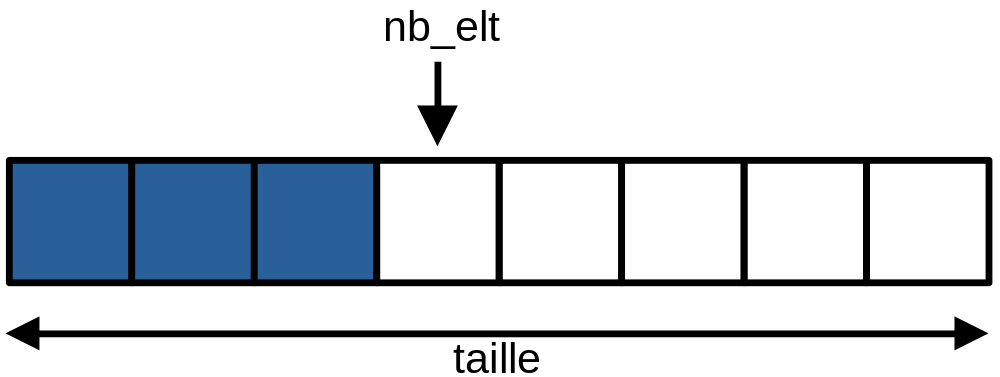
\includegraphics[scale=0.3]{lecon/05-piles_files/piles_tableau.png}
\\

\begin{principe}
	Pour cela, on utilise un indice \texttt{nb\_elt} qui nous indiquera à quelle case du tableau correspond le sommet de la pile, les cases précédentes du tableau contenant les autres éléments empilés.
\end{principe}

\begin{impl}
	On doit soit alors utiliser un tableau de taille fixe (et donc connaître à l'avance le nombre max d'éléments dans la pile)
\end{impl}

\chapter{Implémentations et applications des ensembles et des dictionnaires}
\label{L6}
\dev{Emile Martinez}{}{}{}

\section{Dictionnaire : type abstraits et motivation}


\begin{definition}[Dictionnaire]
	Soit $X$ un ensemble d’éléments appelés valeurs, et $K$ un ensemble d’éléments appelés clés. Un dictionnaire $D$ est une structure de données abstraites ayant les trois opérations :
	
	— $\texttt{Inserer}(D,k,x)$ : insère le couple $(k, x)$ dans $D$, en écrasant un éventuel couple $(k, x')$ préexistant.
	
	— $\texttt{Recherche}(D,k)$ : renvoie la valeur de $x$ telle que $(k, x)$ est dans $D$, si elle existe (peut renvoyer une valeur pas dans $X$ sinon)
	
	— $\texttt{Supprime}(D,k)$ supprime un éventuel couple $(k, x)$ présent dans $D$.
\end{definition} 

\begin{example}
	annuaire téléphonique : les clefs sont les noms des personnes, les valeurs leurs numéros de téléphone
\end{example}

\begin{rem}
	Les dictionnaires sont aussi appelés tableaux associatifs
\end{rem}

\begin{appl}
	Si on a une base de données de personnes, identifiés par un pseudonyme, on peut stocker leur informations dans un dictionnaire.
\end{appl}

\begin{rem}
	C'est ce qui se passe dans une base de données
\end{rem}

\begin{impl}[naive]
	On pourrait stocker tous les éléments dans une liste, sans ordre particulier
\end{impl}

\begin{exercise}
	Implémenter alors les fonctions de bases. Quelles sont leur complexité ?
\end{exercise}

\section{Implémentation}

\subsection{Par des arbres}

\subsubsection{Arbres binaires de recherche (ABR)}

\begin{definition}[ABR]
	Un arbre binaire de recherche (ABR) est un arbre binaire dont les éléments sont munis d'un ordre total et où, pour chaque sous-arbre $N(g, x, d)$, l'élément $x$ est supérieur à tous les éléments de $g$ et inférieur à tous les éléments de $d$.
\end{definition}

\begin{impl}
	On peut implémenter un dictionnaire à l'aide d'un ABR à condition que l'ensemble des clefs soit muni d'un ordre total (On insère les couples (clé, valeur) et l'ordre est sur les valeurs)
\end{impl}

\begin{example} Deux implémentations du même ABR :\\
	\begin{minipage}{0.5\linewidth}
		\begin{tikzpicture}[-, node distance=2cm]
			\node[state] (q0) {10};
			\node[state, below left of = q0] (q1) {8};
			\node[state, below left of = q1] (q2) {5};
			\node[state, below left of = q2] (q3) {3};
			
			\draw (q0) edge[] node{} (q1);
			\draw (q1) edge[] node{} (q2);
			\draw (q2) edge[] node{} (q3);
			
		\end{tikzpicture}
	\end{minipage}\begin{minipage}{0.5\linewidth}
		\begin{tikzpicture}[-, node distance=2cm]
			\node[state] (q0) {5};
			\node[state, below left of = q0] (q1) {3};
			\node[state, below right of = q0] (q2) {10};
			\node[state, below left of = q2] (q3) {8};
			
			\draw (q0) edge[] node{} (q1);
			\draw (q0) edge[] node{} (q2);
			\draw (q2) edge[] node{} (q3);
			
		\end{tikzpicture}
	\end{minipage}
\end{example}

\paragraph{Insertion} Dans un ABR, on insère un élément $x$ en descendant depuis la racine, en prenant le fils gauche ou le fils droit selon si $x$ est plus petit ou plus grand que la racine courante, et en créant un nouveau nœud étiqueté par $x$ lorsque l’on ne peut plus avancer.
	
\paragraph{Recherche} Elle se fait de manière analogue

\paragraph{Suppression} Lorsque le nœud est une feuille ou si le nœud n’a qu’un enfant, alors la transformation est simple. Par contre, si le nœud possède deux enfants, alors il faut retirer le minimum du sous-arbre droit (ou le maximum du sous-arbre gauche) pour le remplacer.

\begin{exercise}
	Implémentation des ABR en OCamL
\end{exercise}

\begin{proposition}
	Soit $\mathcal A$ un ABR à $n$ nœuds et de hauteur $h$. La recherche, l’insertion et la suppression	se font dans le pire cas en $O(h)$ comparaisons. Or un ABR peut être déséquilibré : la hauteur est alors en $O(n)$
\end{proposition}

\subsubsection{Arbres rouge-noir (ARN)}

\begin{definition}
	 Un arbre rouge noir (ARN) est un ABR où chaque nœud porte une couleur rouge ou noir, et qui vérifie les deux propriétés suivantes : \begin{itemize}
		\item la racine est noire 
		\item les potentiels fils d'un nœud rouge sont noirs
		\item pour chaque nœud, tous les chemins menant de ce nœud à une feuille ont le même nombre de nœuds noirs. 
	\end{itemize}
\end{definition}

\begin{proposition}
	\label{06-equilibre}
	Les ARN sont équilibrés ($h = O(\log n)$)
\end{proposition}

\begin{corollary}
	Dans un ARN, on peut effectuer les opérations d'insertion, de recherche et de suppression en $O(h)$, ie $O(\log n)$. 
\end{corollary}

\paragraph{Developpement} Preuve de la propriété \ref{06-equilibre} et présentation de l'insertion dans un ARN

\subsection{Tables de hachage}

\begin{idee}
	Le but ici va être de stocker nos données dans un tableau (d'où le nom tableau associatif). Cela se fait donc en deux étapes : \begin{itemize}
		\item Associer à notre données un nombre (pas trop grand) (appelé hachage) par une fonction appelée fonction de hachage.
		\item Avoir un tableau avec une case par hachage possible, où l'on stocke la donnée
	\end{itemize}
\end{idee}

\subsubsection{Fonction de hachage}

\begin{definition}
	Une fonction de hachage est une fonction $h : K \to \llbracket 0, m-1 \rrbracket$ (avec $m << |K|$)
\end{definition}

\begin{proposition}
	Une fonction de hachage a la propriété du hachage parfait si pour $x \neq y \in K$, $\mathbb P(h(x) = h(y)) = \dfrac{1}{m}$
\end{proposition}

\begin{rem}
	Le hachage parfait veut dire que les valeurs de hachage sont comme pris au hasard dans $\llbracket 0, m-1\rrbracket$. Néanmoins, comme on veut que $h(x)$ vaille toujours la même chose, on ne prend pas de fonctions aléatoires.
\end{rem}

\begin{example}
	On choisit un flottant A. On interprète les bits de données de la structure comme un entier x (en les collant). On prend alors $h(d) = \lfloor A*x \rfloor \mod m$
\end{example}

\subsubsection{Table de hachage}

Il y a trois étapes dans le stockage dans un tableau: \begin{enumerate}
	\item Hacher la valeur et la mettre dans à sa case dans le tableau
	\item Si la case était déjà occupée (collision), stocker la donnée dans une structure annexe
	\item Si le tableau est trop plein, augmenter m (et donc recopier toutes les données).
\end{enumerate}

\begin{example} Schéma où la structure annexe est une liste chaînée pour chaque case\\
	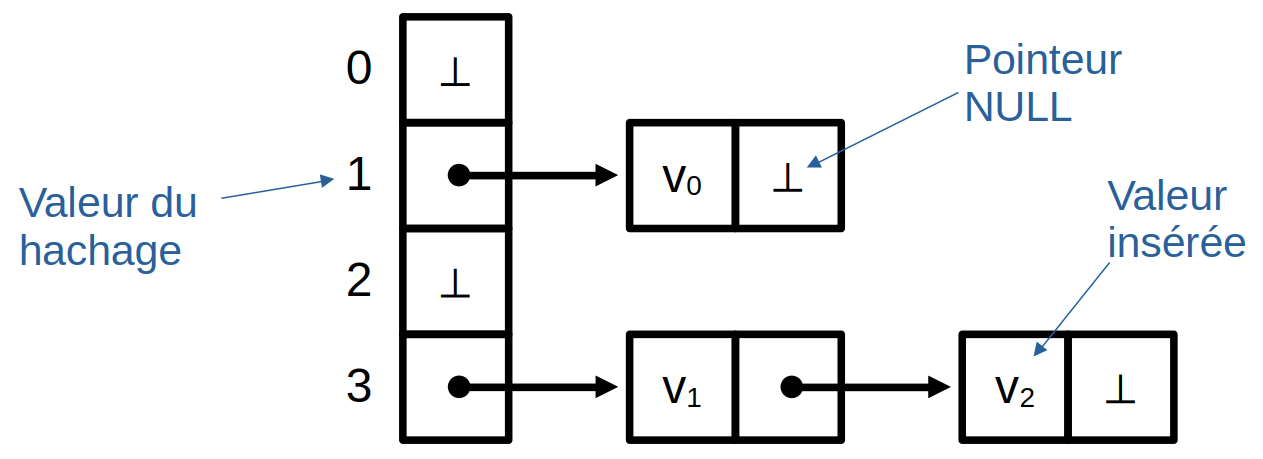
\includegraphics[width = 0.7\linewidth]{lecon/06-ensembles_et_dictionnaires/table_hachage.png}
\end{example}

\begin{com}
	Si on a la place on peut ecrire la remarque, sinon le dire à l'oral que si les abr nécessite un ordre total, la table de hachage nécessite de sérialiser ou de donner directement le hachage
\end{com}

\begin{com}
	Normalement là on pourrait parler de compexité, mais on considère que le tableau \ref{06-tab} suffit.
\end{com}

\section{Ensembles}

\begin{definition}
	Un ensemble est un dictionnaire dans lequel il n'y a pas de clefs. La fonction recherche renvoie donc un booléen qui indique la présence ou non de l'élément. 
\end{definition}

\begin{rem}
	On déduit alors de l'implémentation des dictionnaires, l'implémentation des ensembles
\end{rem}

\begin{com}
	Cette remarque justifie que l'on parle si brièvement des ensembles, et si tard dans la leçon. Beaucoup des choses sur les ensembles se déduisant de celles des dictionnaires
\end{com}

\begin{idee}
	Comme ce sont des ensembles on pourrait également vouloir des opérations ensemblistes comme l'union, l'intersection, etc...
\end{idee}

\begin{impl}
	On peut faire ces opérations sur les structures précédentes en les parcourant (pour l'union, on insère tous les éléments de l'un dans l'autre par exemple)
\end{impl}

\begin{rem}
	Ces opérations réhabilite l'idée de la liste triée
\end{rem}

Récapitulatif des complexités :\\


\begin{tabular}{|l|c|c|c|c|c|}
	\hline \label{06-tab} Structure & Insertion & Suppression & Recherche & union & intersection\\
	\hline liste & $O(n)$ & $O(n)$ & $O(n)$ & $O(n\times m)$ & $O(n \times m)$ \\
	\hline liste triée & $O(n)$ & $O(n)$ & $\log n$ & $O(n+m)$ & $O(n+m)$\\
	\hline ARN & $O(\log n)$ & $O(\log n)$ & $O(\log n)$ & $O(n+m)\log(n+m)$ & $O(\min(n,m) \log(\max(n,m)))$\\
	\hline Table de  & $O(n)$ & $O(n)$ & $O(n)$ & $O(n\times m)$ & $O(n \times m)$ \\
	hachage & $O(1)$ moy. & $O(1)$ moy. & $O(1)$ moy. & $O(n+m)$ moy. & $O(\min(n,m))$ moy. \\ \hline 
\end{tabular}

\begin{exercise}
	Choisir des implémentations en C et les comparer. Si l'on traite les listes triées, ouverture sur les skip listes
\end{exercise}

\section{Application}

\subsection{Dictionnaire d'adjacence}

Soit $G=(S, A)$ un graphe. (où $S = \llbracket 1, n \rrbracket$)\\

On peut représenter $G$ par un tableau de dictionnaire $D$ tq $D[u]$ est un dictionnaire contenant les voisins de $u$\\

\textbf{intérêts :} On a les avantages de la matrice d'adjacence (on detecte rapidement si il y a une arête) et des listes d'adjacence (stockage en |A| et obtention de tous les voisins linéairement).\\

\begin{example}
	Sur un graphe de personnes se connaissant, on sait si A connait B rapidement, mais on n'a pas à stocker tous les false des couples de personnes en se connaissant pas.
\end{example}

\subsection{Mémoïsation}
Supposons que l'on ait une fonction du type
\begin{lstlisting}
fonction (f_args):
    corps de f
    return x
\end{lstlisting}

Il se peut que l'on ait beaucoup d'appels à \texttt f sur les mêmes arguments, comme des fonctions récurisves en programmation dynamique. En s'inspirant de cette dernière, on peut alors ne faire qu'une fois les appels sur chaque argument grâce à un dictionnaire :

\begin{lstlisting}
fonction f(args):
    Si args est dans dictionnaire:
        renvoyer dictionnaire[args]
    Sinon:
        corps de f
    dictionnaire[args] = x
    renvoyer x
\end{lstlisting}

\subsection{Autres applications}

\begin{com}
	On peut dire à l'oral que en gros, utiliser un dictionnaire est un peu équivalent à $f : K \to \llbracket 1, K \rrbracket$. (c'est plus que simplement le fait logique que, par un tableau classique, c'est équivalent)
\end{com}

Les dictionnaires et les ensembles servent dès que l'on veut accéder rapidement à un élément dont la structure n'est pas un entier.

\begin{example}
	En algorithmique du texte, pour associer des valeurs à des chaînes de caractère (Huffman, Boyer-Moore)
\end{example}

\begin{example}
	Quand on fait un parcours de graphe dont les sommets ne sont pas $\llbracket 1, n \rrbracket$ on peut utiliser un ensemble pour savoir quels éléments on a déjà parcouru.
\end{example}

\begin{com}
	On peut soit insister à l'oral sur cet exemple, soit en faire une sous partie, du fait que c'est une application pour les ensembles
\end{com}

Mais on peut les retrouver également dans beaucoup de domaines comme en bases de données, et dès que l'on manipule un nombre faible de valeur comparés à l'ensemble des valeurs possibles.

\textbf{Développement :} Amélioration du tri par comptage par l'usage de dictionnaires.

\chapter{Accessibilité et chemins dans un graphe. Applications}
\label{L7}
\dev{Emile Martinez}{}

\begin{com}
	Les applications sont éparpillées tout le long de la leçon, et relativement peu développer, donc il peut-être rentable des les souligner pendant la défense de plan.
\end{com}

\section{Definition}

\begin{definition}[chemin]
	Dans un graphe orienté $G$ (resp. non orienté) on appelle chemin de longueur $\lambda$ une suite de $(\lambda + 1)$ sommets $(s_0, \, s_1, \,\dots, \, s_\lambda)$
\end{definition}

\begin{rem}
	Par convention, on dit qu’il y a un chemin de longueur 0 de tout sommet vers lui-même.
\end{rem}

\begin{rem}
	Dans un graphe non-orienté, les chemins sont aussi appelés chaînes.
\end{rem}

\begin{appl}
	Dans un graphe de flot de contrôle, le critère tous les chemins consiste à trouver des tests qui font tous les chemins possibles du graphe
\end{appl}

\begin{com}
	Une première application, dont on ne parle pas beaucoup plus parce que ca a pas grand chose a voir. Donc les chemins servent là, mais la théorie derrière n'est pas intéressante par la théorie des graphes. Illustre simplement la diversité de l'utilisation des graphes.
\end{com}

\begin{com}
	On peut mentionner que ca fait déjà une première application
\end{com}

\begin{definition}[chemin élémentaire]
	Un chemin est dit élémentaire s’il ne contient pas plusieurs fois le même sommet.
\end{definition}

\begin{com}
	Par manque de place, cette définition peut être enlevé
\end{com}

\begin{definition}[circuit/cycle]
	Dans un graphe orienté (resp. non orienté), un chemin $(s_0, \, \dots, \, s_\lambda)$ dont les $\lambda$ arcs (resp. arêtes) sont distincts deux à deux et tels que $s_0 = s_\lambda$ , est un circuit (resp. un cycle).
\end{definition}

\begin{example}
	On dit qu'un circuit est hamiltonien si il passe par tous les sommets une et une seule fois. Décider de l'existence d'un tel circuit dans un graphe est NP-complet (i.e. dur)
\end{example}

\begin{exercise}
	On dit qu’un graphe non orienté est Eulérien s’il existe un cycle passant par chaque arête exactement une fois. Montrer qu’un graphe est eulérien si et seulement si tous ses sommets sont de degré pair.
\end{exercise}

\begin{com}
	Ces deux choses là peuvent être présenter comme des formes d'applications, du moins d'application des définitions (il semble important que la NP-complétude de quelque chose soit mentionné dans cette leçon)
\end{com}

\begin{definition}[accessibilité]
	Étant donné un graphe $G$ (orienté ou non) et deux sommets $s$ et $t$, on dit que $t$ est accessible depuis $s$ s’il existe un chemin allant de $s$ à $t$ dans $G$.
\end{definition}

\section{Accessibilité}

\subsection{Tri topologique}

\begin{definition}[tri topologique]
	Étant donné un graphe orienté $G = (S,A)$, on dit que $\sigma : S \to \llbracket 1,  |S| \rrbracket$ est un tri topologique si $(s,t) \in A \implies \sigma(s) < \sigma(t)$
\end{definition}

\begin{corollary}
	Soit $\sigma$ un tri topologique sur $G$. Pour $s, t \in S$, si il existe un chemin de $s$ à $t$, alors $\sigma(s) \leq \sigma(t)$
\end{corollary}

\begin{proposition}
	$G$ est acyclique si et seulement si $G$ admet un tri topologique.
\end{proposition}

\begin{proof}[pour le sens direct]
	On montre par l'absurde par récurrence qu'un graphe acyclique a un sommet source.\\
	On montre par récurrence la proposition sur $|S|$
\end{proof}

\begin{algo}Construction d'un tri topologique
	\begin{itemize}[label=$\bullet$]
		\item Créer une pile vide
		\item Faire un parcours en largeur postfixe de G en appliquant la fonction empile
		\item Renvoyer la pile
	\end{itemize}
\end{algo}

\begin{appl}
	Ordonnancement de tâches
\end{appl}

\begin{definition}
	Soit $T=\{ t_1, \, \dots, \, t_n \}$ un ensemble de tâches d'un ordinateur et $C = T^2$ un ensemble de contraintes $((t_i, t_j) \in C$ veut dire que $t_i$ doit être fait avant $t_j$). Un ordonnancement de ces tâches est un ordre d'éxécution de ces tâches.
\end{definition}

\begin{proposition}
	On peut trouver un ordonnancement en temps linéaire
\end{proposition}

\begin{proof}
	On prend le graphe $(T, C)$ est on fait un tri topologique.
\end{proof}

\subsection{Connexité}

\begin{proposition}
	La relation «il existe un chemin de $s$ à $t$ et de $t$ à $s$» est une relation d'équivalence.
\end{proposition}

\begin{exercise}
	Montrer que le graphe quotienté par cette relation d'équivalence est acyclique
\end{exercise}

\begin{com}
	Ici on introduit le DAG des classes des composantes (fortement) connexes. On peut néanmoins dire que suivant le niveau de la classe, il est très probable que le terme quotienté ne soit pas maitrisé. Donc la on le met par concision, au cas où il aurait déjà était vu en maths (hors programme en maths), mais en vrai on pourrait périphraser et faire des définitions. De plus la c'est un plan, donc on dit ce qu'on ferait dans l'exercice, pas tout l'énoncé rigoureux.
\end{com}

\begin{definition}
	Dans un graphe non orienté (resp. orienté), les classes d'équivalence de cette relation sont appelés composantes connexes (resp. fortement connexes).\\
	Si il n'y a qu'une seul classe, le graphe est dit connexe (resp. fortement connexe)
\end{definition}


\begin{com}
	On prend ca comme déf et non pas la propriété suivantes en ayant défini connexe comme un chemin de tous le monde à tout le monde, pour avoir une définition plus explicites et naturelles que de passer par la maximalité. Néanmoins, cela nécessite l'abstraction de la classe d'équivalence (vue en maths). Si la classe est faible, on peut faire tout ca plus avec les mains.
\end{com}

\begin{exercise}
	Dans un graphe connexe, deux chemins élémentaires maximaux ont un nœud en commun.
\end{exercise}

\begin{proposition}
	Une composante connexe (resp. fortement connexe) est un sous-graphe connexe (resp. fortement connexe) maximal.
\end{proposition}

\begin{algo} \enspace\\
	\begin{algorithm}[H]
		\Tq{un sommet n'est pas visité}{
		    Créer une nouvelle composante connexe\\
			Parcourir le graphe des sommets non visités depuis un sommet v non visité en ajoutant a la composante tous les sommets que l'on croise
		}
		\caption{Calcul des composantes connexes (cas non orienté)}
	\end{algorithm}
\end{algo}

Pour les composantes fortement connexes, il faudra plus qu'un simple parcours.

\begin{algo}\enspace \\
	\begin{algorithm}[H]
		\caption{Algorithme de Kosaraju}
		Appliquer l'algorithme de construction d'un tri topologique (meme si le graphe a des cycles)\\
		Prendre $G^T$ le graphe transposé de $G$ (i.e., $(u,v)$ devient $(v,u)$)
		\Pour{i allant de 1 à n}{
			Si $\sigma(i)$ n'a pas déjà été visité\\
			Créer une nouvelle composante fortement connexe\\
			Visiter $G^T$ depuis $\sigma(i)$ en ajoutant les sommets visités non encore attribués\\
		}
	\end{algorithm}
\end{algo}

\begin{proposition}
	Cet algorithme construit les composantes fortement connexes en temps linéaire
\end{proposition}

\begin{definition}
	Le problème 2-SAT est le problème de savoir si étant donné $n$ variables $x_1, \,\dots ,\, x_n$ et $p$ clauses $C_1, \,\dots ,\, C_p$ de taille 2 sur $x_1,\, \dots, \, x_n$, $\varphi = \bigwedge\limits_{i=1}^p C_i$ est satisfiable
\end{definition}

\textbf{Developpement :} Résolution en temps linéaire de 2-SAT.

\section{Plus court chemin}

\begin{definition}[graphe pondéré]
	Un graphe pondéré est un graphe $G = (S, A)$ muni d’une fonction de poids $w : A \to Z$.\\
	Le poids d’un chemin est alors défini comme la somme des poids des arêtes qui le compose.
\end{definition}

\begin{rem}
	On peut étendre $w$ à $S^2$ en posant $w(u, v) = +\infty$ lorsque $(u, v) \notin A$.
\end{rem}

\begin{definition}
	Dans un graphe $G$, un plus court chemin (pcc) de $u$ à $v$ ($u,v\in S$) est un chemin de poids minimal de $u$ à $v$
\end{definition}

\begin{rem}
	Si les poids sont unitaires, on peut trouver le pcc entre deux sommets $u$ et $v$ en faisant un parcours en largeur depuis $u$.
\end{rem}

\begin{com}
	On considère les parcours déjà vu (servant dans bien d'autres contextes que les chemins dans les graphes). Ici on fait simplement le lien, et on illustre la notion. On pourrait également le faire sur un exemple au tableau, et essayer de le faire devnier aux élèves (lien entre différentes parties du cours)
\end{com}

\subsection{D'un sommet à tous les autres}

Lorsque la fonction de poids est à valeur dans $\N$, on peut utiliser l'algorithme de Dijkstra.

\begin{algo} 
	\enspace \\
	\begin{algorithm}[H]
		\caption{$dijkstra(G, S)$}
		$distance \gets $ tableau de taille $|S|$ initialisé à $+\infty$\\
		$distance[s] \gets 0$\\	
		$F \gets FilePriorite()$\\
		$Inserer(F, s, 0)$\\
		\Tq{$\neg estVide(F )$}{
			$u, du \gets ExtraireMin(F)$\\
			\Pour{$v \in N(u)$}{
				$d \gets du + w(u, v)$\\
				
				\Si{$d < distance[v]$}{
					\eSi{$distance[v] = +\infty$}{
						$Inserer(F ,v,d)$
					}{
						$DiminuerPriorite(F ,v,d)$\\
						$distance[v] \gets d$
					}
				}
			}
		}
		\Retour $distance$
	\end{algorithm}
\end{algo}


\begin{proposition}
	L’algorithme de Dijkstra réalise au plus $|S|$ appels à $Inserer$ et $ExtraireMin$, et $|A|$ appels à $DiminuerPriorite$.\\
	Donc avec un tas min, on obtient $O(|A| \times \log |S|)$
\end{proposition}

\begin{rem}
	Si la structure d'entrée est une matrice d'adjacence, on peut faire l'algorithme en $O(n^2)$ sans structure particulière pour $F$.
\end{rem}

\begin{rem}
	Lorsque la fonction de poids est à valeur dans $\mathbb Z$ et que le graphe ne contient aucun circuit absorbant, on peut utiliser l'algorithme de Bellman-Ford.
\end{rem}

\begin{appl}
	Détection des cycles absorbants.
\end{appl}

\begin{rem}
	Si l'on souhaite seulement le plus court chemin entre deux points, on peut utiliser l'algorithme A* (Dijkstra + heuristique du chemin restant).
\end{rem}

\subsection{De tous les sommets à tous les sommets}

Lorsque le graphe ne contient aucun cycle absorbant, l'algorithme de Floyd Warshall calcule les plus courts chemins entre toute paire de sommets de $S=\{1, \, \dots , \,n\}$ par programmation dynamique. \begin{itemize}[label=$\star$]
	\item \textbf{Sous-problèmes :} $d^{(k)(i,j)}$ la distance du pcc de $i$ à $j$ avec seulement $\llbracket 1, k \rrbracket$ comme sommets intermédiaires
	\item \textbf{Relation de récurrence}
	$$ \begin{array}{l}
		d^{(0)}(i,j) = w(i,j)\\
		d^{(k+1)}(i,j) = \min\left(d^{(k)}(i,j), \enspace d^{(k)}(i,k) + d^{(k)}(k, j)\right)
	\end{array} $$
	\item \textbf{Résolution :} On résout sur $S^2$ à $k$ croissant
\end{itemize}

\begin{proposition}
	Floyd Warshall est en $O(n^3)$
\end{proposition}

\begin{rem}
	Si les poids sont positifs, appliquer dijkstra à chaque sommet nous donne $O(n \times |A| \times \log n)$
\end{rem}

\begin{rem}
	Cette algorithme utilise une matrice d'adjacence (algorithme centralisé)
\end{rem}

\begin{algo}
	Si on a des listes d'adjacence (algorithme décentralisé/distribué), on peut utiliser l'algorithme de Bellman Ford
\end{algo}

\begin{appl}
	Routage des paquets d'un réseau par le protocole IP avec l'algorithme de Bellman Ford.
\end{appl}

\noindent \textbf{Developpement :} Presentation et terminaison de l'algorithme de Bellamn Ford.


\begin{com}
	On a fait une leçon sur les graphes, sans aucun dessin de graphes. En vrai, il pourrait y en avoir sur des exemples, et puis les schémas ne sont pas absolument necessaires pour illustrer la plupart des concepts, dont surtout la formalisation est imporante (la def d'un chemin est explicite).
\end{com}




\chapter{Algorithme de tri. Exemple, Complexité et Applications}
\label{L8}
\dev{Emile Martinez}{}

\section{Introduction}

\begin{definition}
	Un algorithme de tri prend en entrée un liste d'éléments $E$ muni d'un ordre total $\leq$ ( mais dont on peut se passer de l'antisymétrie) et renvoie o=une liste $S$ telle que : \begin{enumerate}
		\item elle contient exactement les éléments de $E$
		\item les éléments de $S$ apparaissent dans l'ordre croissant
	\end{enumerate}
\end{definition}

\begin{appl}
	Pourquoi trier ? Cela permet de simplifier des opérations (min, max, recherche, etc...)
\end{appl}

\begin{exercise}
	Chercher à la main un mot dans une liste triée et non triée.
\end{exercise}

\begin{com}
	\label{08-activite}
	On peut faire cet exercice en seconde. Avec éventuellement le fait de comparer deux listes de mots. Tout ca pour voir l'intérêt du tri. Ensuite on peut leur demander comment faire pour trier, permettant de faire émerger des algorithmes sans le formalismes nécessaires. Et suivant le format des mots, on obtiendra probablement des choses différentes (une liste écrit sur un papier -> tri par sélection, des cartes avec les mots -> tri par insertion, tri a bulle, voir même du tri par paquet).
	
	Ainsi on peut faire de l'informatique sans l'écueil de  l'apprentissage de la syntaxe python qui bloque beaucoup d'élèves.
\end{com}

\begin{definition}[Propriétés des tris]
	\begin{itemize}[label=$\bullet$]
		\item en place : Utilise $O(1)$ espace en plus de l'espace des données d'entrées
		\item stable : Si $E[i] \leq E[j]$ et si $E[j] \leq E[i]$, avec $i < j$, dans $S$, $E[i]$ apparaîtra avant $E[j]$
		\item en ligne : on peut trier les données même si elles arrivent au fur et à mesure
		\item parallélisable : on peut diviser le travail sur plusieurs fils.
	\end{itemize}
\end{definition}

\section{Tri quadratiques}

\subsection{Tri par sélection}

\begin{minipage}{0.5\linewidth}
	\begin{algorithm}[H]
		\caption{$Tri\_par\_selection(E)$}
		$S \gets [\,]$\\
		\Pour{$i$ allant de $1$ à $|E|$}{
			Extraire $mini$, le minimum de $E$\\
			Ajouter $mini$ à la fin de $S$
		}
		\Retour $S$
	\end{algorithm}
\end{minipage} \begin{minipage}{0.5\linewidth}
	\begin{example} \normalfont
		\begin{center}$E = [4, \, 3, \, 6, \, 1]$\\
			\begin{tabular}{|c|c|c|c|}
				\hline $i$ & $E$ & $m$ & $S$\\
				\hline $\times$ & [4, 3, 6, 1] & $\times$ & []\\
				\hline 0 & [4, 3, 6] & 1 & [1]\\
				\hline 1 & [4, 6] & 3 & [1, 3]\\
				\hline 2 & [6] & 4 & [1, 3, 4]\\
				\hline 3 & [] & 6 & [1, 3, 4, 6]\\
				\hline
			\end{tabular}\\
			$S = [1, \, 3, \, 4, \, 6]$
		\end{center}
	\end{example}
\end{minipage}

\begin{com}
	Cet exemple peut être remplacer par simplement : «Exemple : mettre un exemple d'execution de l'algorithme» si on manque de place
\end{com}

\begin{proposition}
	\enspace\\
	\begin{itemize}[label=$\star$]
		\item Terminaison : l'algorithme n'utilise que des boucles bornées
		\item Correction : Invariant de boucle «$S$ est trié et contient les $i$ plus petits de $E$»
		\item Cout : environ $|E|^2$
	\end{itemize}
\end{proposition}

\begin{proposition}
	Le tri par sélection est stable (si on extrait le premier min) mais ni en ligne, ni en place, ni facilement parallélisable
\end{proposition}

\begin{exercise}
	Réécrire le tri pour qu'il soit en place. Qu'advient-il de la stabilité ?
\end{exercise}

\subsection{Tri par insertion}

\begin{algorithm}[H]
	\caption{$Tri\_par\_insertion$}
	\Pour{$i$ allant de $0$ à $|E|-1$}{
		$v \gets E[i]$\\
		$j \gets i-1$\\
		\Tq{$j > 0$ et $E[j] > E[j+1]$}{
			Échanger $E[j]$ et $E[i]$\\
			$j \gets j-1$\\
		}
	}
	\Retour{E}
	\label{08-inser}
\end{algorithm}

\begin{proposition}
	L'algorithme \ref{08-inser} est stable, en place et en ligne.
\end{proposition}

\begin{rem}
	Il est difficilement parallélisable
\end{rem}

\begin{exercise}
	Quel est la complexité de cet algorithme
\end{exercise}

\subsection{Recherche Dichotomique}

\begin{algorithm}[H]
	\caption{$Recherche\_dichotomique(E, x)$}
	\eSi{$|E| = 0$}
	{
		\Retour{Faux}
	}
	{
		$a \gets 0, \, b \gets |E|-1, \, m \gets \left\lfloor \dfrac{a+b}{2} \right\rfloor$\\
		\Tq{$E[m] \neq x$ et $(b-a)>0$}{
			\eSi{$E[m] < x$}
				{$a \gets m+1$}
				{$b \gets m-1$}
			$m \gets \left\lfloor \dfrac{a+b}{2} \right\rfloor$
		}
		\eSi{$E[m] = x$}
			{\Retour{Vrai}}
			{\Retour{Faux}}
	}
\end{algorithm}

\noindent\textbf{Terminaison :} variant de boucle : «$b-a$»\\
\textbf{Correction :} invariant de boucle : «Si $x$ est dans $E$ alors son indice est entre $a$ et $b$»\\
\textbf{Cout :} nombre de bit de $|E|$

\begin{impl}
	Implémentation en Python et comparaison avec la recherche linéaire
\end{impl}

\begin{exercise}
	Écrire une version récursive de l'algorithme
\end{exercise}

\section{Tri efficace}

\subsection{Tri fusion}

\begin{definition}
	L'algorithme de tri fusion est un algorithme de tri qui repose sur deux opérations : \begin{itemize}
		\item $partitionner(L)$ : coupe $L$ en deux listes de taille équivalente $L_1$, $L_2$
		\item $fusion(L_1, L_2)$ : avec $L_1$ et $L_2$ deux listes triées, renvoie $L3$ la liste triée contenant tous les éléments de $L_1$ et $L_2$.
	\end{itemize}
\end{definition}

\begin{algorithm}[H]
	\caption{fusion($L_1$, $L_2$)}
	$res \gets []$\\
	$i,j \gets 0$\\
	\Tq{
		$i < |L_1|$	et $j < |L_2|$
	}{
		\eSi{$L_1[i] < L_2[j]$}{
			$res$.ajouter($L_1[i]$) \\
			$i \gets i + 1$
		}{
			$res$.ajouter($L_2[j]$) \\
			$j \gets j + 1$
		}
	}
	Ajouter le reste de $L_1$ et de $L_2$ à $res$\\
	\Retour{$res$}
\end{algorithm}

\begin{algorithm}[H]
	\caption{tri\_fusion($L$)}
	$n \gets |L|$\\
	\Si{$n\leq 1$}{
		\Retour{$L$}
	}
	$L_1, L_2 \gets$ partionner($L$)\\
	\Retour{fusion( tri\_fusion($L_1$), tri\_fusion($L_2$) )}
\end{algorithm}

\textbf{Developpement :} Correction totale du tri fusion

\begin{proposition}
	Ce tri est stable mais pas en place. Parallélisable mais pas en ligne.
\end{proposition}

\textbf{Complexité :} $C(n) = 2\times C(\frac{n}{2})$ donc $C(n) = O(n \times \log n)$

\subsection{Tri rapide}

\begin{idee}
	Choisir un élément appelé pivot et mettre à gauche tous les éléments plus petit, à droite tous les plus grands, puis à trier cette partie à droite et à gauche.
\end{idee}

\begin{algorithm}
	\caption{$tri\_rapide(L, debut, fin)$}
	\Si{$debut \geq fin -1$}
		{\Retour{$L$}}	
	$pivot \gets L[0]$\\	
	$i \gets debut$\\
	$j \gets fin$\\
	\Tq{$i < j$}
	{
		\eSi{$L[i+1] \leq pivot$}
		{
			échanger $L[i+1]$ et $L[i]$\\
			$i \gets i+1$
		}{		
			échanger $L[i+1]$ et $L[j]$\\
			$j \gets j - 1$
		}
	
		$tri\_rapide(L, debut, i-1)$\\	
		$tri\_rapide(L, i+1, fin)$\\
	}
\end{algorithm}

\begin{com}
	Par manque de place, on peut remplacer l'écriture de cet algorithme par un dessin expliquant l'idée, et mettre son écriture en exo
\end{com}

\begin{proposition}[Complexité]
	\begin{itemize}
		\item pire des cas : $O(n^2)$
		\item meilleur cas : $O(n\log n)$
		\item cas moyen avec pivot aléatoire : $O(n\log n)$
		\item pire cas avec pivot astucieux : $O(n\log n)$
	\end{itemize}
\end{proposition}

\begin{proposition}
	Ce tri est en place, non stable, non en ligne mais parallélisable
\end{proposition}

\begin{com}
	On peut éventuellement mentionner que dans beaucoup d'implémentation, pour le pivot on prend quelques valeurs (exemple 5) et on prend la médiane de ces valeurs là (ainsi on est quasiment jamais dans le pire cas et sans devoir calculé la médiane). Mais avec l'avantage de rester en place
\end{com}

\begin{com}
	Pour le caractère en place, il faut discuter de la pile d'appel. A priori, l'espace supplémentaire utilisé est en $O(\log n)$ (voir $O((\log n)^2$ si on considère le stockage des indices mais là on part un peu trop loin)) et non $O(1)$, mais on s'en contente souvent.
\end{com}

\begin{exercise}
	Écrire une version stable de ce tri. Préserve-t-on le caractère en place.
\end{exercise}

\subsection{Tri par tas}

\begin{algorithm}[H]
	\caption{$tri\_tas(L)$}
	Insérer les éléments de $L$ dans un tas initialement vide\\
	Extraire successivement l'élément minimum du tas.
\end{algorithm}

\begin{exercise}
	Quelles propriétés vérifie ce tri ?
\end{exercise}

\subsection{Minoration de la complexité du tri}

\begin{proposition}
	On ne peut pas trier n éléments avec une complexité inférieure à $n-1$
\end{proposition}

\begin{proposition}
	Un algorithme de tri par comparaison aura une complexité pire cas au mieux $O(n \log(n))$
\end{proposition}

\begin{proof}
	S'intéresser à l'arbre des chemins que prend l'algorithme en fonction du résultat des comparaisons.
\end{proof}

\begin{rem}
	Si on ne trie pas par comparaison, on peut avoir des complexités plus faibles. Par exemple, si E ne contient que des entiers entre 0 et 9, on peut simplement compter le nombre de 0 et de 9 puis reconstruire là dessus le tableau trié.
\end{rem}

\textbf{Développement :} Amélioration du tri par comptage avec des dictionnaires

\section{Application}

\subsection{Algorithmes gloutons}

\begin{definition}
	Un algorithme glouton est un algorithme qui résout un problème d'une entrée $E$ de la forme : \begin{itemize}
		\item on trie les éléments de $E$
		\item on construit une solution en les parcourant, sans revenir en arrière
	\end{itemize}
\end{definition}

\begin{example}
	\label{08-gymnase}
	On a $n$ évènements sportifs ayant lieu respectivement entre les dates $d_i$ et $f_i$ ($i \in \N$) ayant chacun besoin d'un gymnase. Comment allouer des gymnases à des évènements pour utiliser le moins possible de gymnase ? \\
	
	Algorithme glouton :\begin{enumerate}
		\item Trié les évènements par $d_i$ croissant (impliquant souvent de trier)
		\item Mettre chaque évènement dans le premier gymnase vide (peut en être un nouveau)
	\end{enumerate}
\end{example}

\begin{proposition}
	Le glouton de l'exemple \ref{08-gymnase} renvoie une solution optiamle (minimisant le nombre de gymnases)
\end{proposition}

\begin{exercise}
	Écrire un algorithme glouton pour le problème de rendu de monnaie
\end{exercise}

\begin{definition}
	Un arbre couvrant minimal d'un graphe pondéré est un sous graphe connexe acyclique de poids minimal
\end{definition}

\begin{algorithm}[H]
	\caption{$kruskal$}
	\Entree{$L$ liste d'arêtes}
	\Sortie{Arbre couvrant de poids minimal}
	Trier $L$\\
	$res \gets []$
	\Pour{$a \in L$}{
		\Si{$\{a\}\cup res$ n'ajoute pas de cycles}{
			$res \gets res \cup \{a\}$
		}
	}
	\Retour{$res$}
\end{algorithm}

\begin{exercise}
	Proposer des algorithmes gloutons pour la coloration de graphe. Sont-ils optimaux ?
\end{exercise}

\subsection{Implémentation des ensembles}

\begin{com}
	Cette partie fait un peu écho à l'activité mentionner dans le commentaire \ref{08-activite}
\end{com}

\begin{proposition}
	On peut implémenter les ensembles par des listes, par des listes triées, par des listes que l'on trie pour l'union et l'intersection. On obtient alors les complexités suivantes :\\ \normalfont \begin{tabular}{|l|c|c|c|c|}
		\hline Structure & Insertion & Suppression & Recherche & union / intersection\\
		\hline liste & $O(n)$ & $O(n)$ & $O(n)$ & $O(n\times m)$ \\
		\hline liste triée & $O(n)$ & $O(n)$ & $\log n$ & $O(n+m)$ \\
		\hline liste avec tri & $O(1)$ & $O(n)$ & $O(n)$ & $O((n+m) \log(\min(n, m)))$ \\
		\hline
	\end{tabular}
\end{proposition}

\begin{exercise}
	Proposer une implémentation mélangeant les listes triées et les listes avec tri ayant de meilleur complexité
\end{exercise}

\begin{com}
	On s'attend ici à ce que on aient d'une part les éléments déjà triés, de l'autre les éléments pas encore, et on ne trie que quand on fait l'union ou l'intersection (ou éventuellement la recherche) en triant les éléments pas encore triés, puis en fusionnant (cf tri fusion) les deux listes.
\end{com}

\chapter{Algorithmique du texte. Exemples et applications.}
\label{L9}
\dev{Emile Martinez}{}

Un auteur envoie son manuscrit à un éditeur. Il commence par compresser le texte. A la réception, l'éditeur compare le manuscrit à d'autres ouvrages pour vérifier qu'il n'y a pas plagiat. Il peut ensuite chercher un motif dans le texte.

\begin{com}
	Cela justifie l'ordre dans lequel on a mis nos parties. De plus, suivant le niveau du cours, on pourrait inaugurer chaque partie en rappelant quelle partie de ce contexte cela concerne. Mais là le niveau (MPI) est un peu élevé pour s'apesentir sur ce genre de choses
\end{com}

\textbf{Notation :} On prend les conventions de slicing de python


\begin{com}
	Il n'y a pas de partie application car souvent les applications sont directes depuis les algorithmes. Ainsi on les dissémine illustrant directement le concept	
\end{com}


\section{Encodage et compression}

\subsection{Encodage par lettre}

\begin{definition}[Algorithme de compresssion]
	Un algorithme de compression sans perte est la donnée d'une fonction $f : \Sigma^* \to \Sigma^*$ injective (il existe un unique décodage). 
\end{definition}

\begin{algo}[Codage préfixe]
	\enspace
	\begin{enumerate}
	\item Prétraitement : On construit un arbre binaire $\mathcal A$ qu’on appelle arbre de Huffman dont les feuilles sont les lettres $c \in \Sigma$.
	
	\item Compression : On code chaque lettre c par une suite de 0 et 1 correspondant au chemin (0 : gauche, 1 : droite) de la racine à la feuille contenant c dans $\mathcal A$.
	
	\item Décompression : On décode une suite de 0 et 1 en parcourant le chemin correspondant dans $\mathcal A$.
	\end{enumerate}
\end{algo}

\begin{algo}[Codage de Huffman]
	\label{09-Huff}
	\normalfont On note $f_a$ la fréquence du caractère $a$ dans le texte et on note $f_{\mathcal A} = \sum\limits_{a \in \mathcal A} f_a$\\
	\begin{algorithm}[H]
		Créer une forêt $\mathcal F$ d'arbres binaires réduits à un noeud $(a, f_a)$\\
		\Tq{$|\mathcal F| > 1$}
		{
			Extraire de $\mathcal F$ les arbres $\mathcal A_1$ et $\mathcal A_2$ de plus petites fréquences \tcp{$f_{\mathcal A_1} <= f_{\mathcal A_2}$ à la racine}
			Insérer un arbre de racine $f_{\mathcal A_1} + f_{\mathcal A_2}$ ayant pour fils $\mathcal A_1$ et $\mathcal A_2$ dans $\mathcal F$
		}
		\Retour{$\mathcal A_H$ tel que $\mathcal F = \left\{\mathcal A_H\right\}$}
	\end{algorithm}
\end{algo}

\begin{com}
	Mentionner à l'oral qu'on ferait le lien avec le fait que c'est un algorithme glouton sur les arbres unifiant ceux de fréquences des lettres agrégés minimal.
\end{com}

\begin{theorem}
	L'arbre construit par le codage de Huffman \ref{09-Huff} minimise la quantité $S = \sum\limits_c\in \Sigma f_c d_c$ où $d_c$ est la profondeur du caractère $c$ dans l'arbre. 
\end{theorem}

\begin{idee}
	Cela revient à dire que l'algorithme de Huffman est optimal parmi les codages préfixes
\end{idee}

\begin{exercise}
	Quelle structure pour $\mathcal F$ dans l'algorithme \ref{09-Huff} ? Quelle complexité alors ?
\end{exercise}

\subsection{Encodage par séquences}

\begin{idee}
	On va associer un code à une séquence de lettres (ou motifs)
\end{idee}

\begin{rem}
	Pour cela, on peut utiliser le codage de Huffman, en prenant comme alphabet les mots apparaissant dans le livre. Mais on peut faire quelque chose de spécifique aux séquences, mais moins spécifiques à un livre (car ici le caractère " " comme délimitateur est arbitraire).
\end{rem}

\begin{com}
	Si on manque de places, on peut faire cette remarque uniquement à l'oral
\end{com}

\begin{idee}
	L'agorithme LZW détermine un codage dans un dictionnaire $d$ au fur et à mesure de la lecture du texte (algorithme online). On va coder certains motifs (groupement de lettres consécutives) présents dans le texte.
\end{idee}

\begin{algo}[Compression par LZW]
	\enspace \\
	\begin{algorithm}[H]
		Initialement, les lettres de $\Sigma$ sont codées par un entier (par ex. avec le code ASCII).\\
		$m \gets ''$\\
		\Tq{il reste du texte $s$ à coder}
		{
			Retirer le plus long préfixe $w$ de $s$ qui soit dans $d$\\
			Ajouter le codage de $w$ à la fin de $m$\\
			$w' \gets w$ concaténé avec la prochaine lettre de $s$\\
			Ajouter un nouveau codage pour $w'$ dans $d$
		}
		\Retour{m}
	\end{algorithm}
\end{algo}

\begin{rem}
	Pour la décompression, il n'est pas nécessaire de transmettre le dictionnaire car on peut le reconstruire à la volée. 
\end{rem}

\begin{appl}
	Le format de fichier .zip compresse un dossier en utilisant (entre autre) les algorithmes de Huffman et LZW. 
\end{appl}

\textbf{Développement :} Présentation de la compression et de la décompression de l'algorithme LZW

\section{Comparaison}

\subsection{Plus longue sous-suite commune (PLSSC)}

\begin{definition}[Problème PLSSC]
	Soit $x, y \in \Sigma^*$. Une plus longue sous-suite commune à $x$ et $y$, noté $PLSSC(x,y)$ est $argmin \left\{k \: \big/ \: \exists i,j : x[i:i+k] = y[j:j+k]\right\}$
\end{definition}

\begin{appl}
	Ce problème correspond au fait de trouver des morceaux d'ADN communs entre deux séquençages.
\end{appl}

\begin{example}
	Pour $x = 'patate'$ et $y = 'frites'$ on a $'te'$
\end{example}

\begin{algo}[Brute force]
	On essaie toutes les séquences possibles $\to$ exponentiel
\end{algo}

\begin{algo}[programmation dynamique]
	\label{09-PLSCC}
	On considère les sous-problèmes  $c_{i,j} = \left| PLSSC(x[:i], y[:j]) \right|$.\\
	On a alors $c_{i,j} = \left\{
	\begin{array}{ll}
		0 & \text{si } i = 0 \text{ ou } j = 0 \\
		c_{i-1, j-1} & \text{si } x[i-1] = y[j-1]\\
		\max(c_{i-1, j}, c_{i, j-1}) & \text{sinon} \\
	\end{array}\right.$
\end{algo}

\begin{proposition}
	L'algorithme \ref{09-PLSCC} calcule $PLSSC(x, y)$ en $O(|x| \times |y|) $
\end{proposition}

\begin{rem}
	Pour obtenir la sous suite, on sauvegarde d'où l'on vient pour pouvoir reconstruire la solution
\end{rem}

\subsection{Distance entre deux chaînes}

\begin{definition}[distance]
	Une distance sur un ensemble $E$ est une application $d : E^2 \to R^+$ tq :
	$$\begin{array}{ll}
		d(x,y) = d(y,x) & \text{(symétrie)}\\
		d(x,y) = 0 \equiv x = y & \text{(séparation)}\\
		d(x, z) <= d(x,y) + d(y, z) & \text{(inégalité triangulaire)}
	\end{array}
	$$
\end{definition}

\begin{definition}[Distance de Hamming]
	La distance de Hamming entre deux chaines de caractères de même taille est le nombre de caractères distincts.
\end{definition}

\begin{appl}
	Dans un protocole réseau, on peut ajouter des bits de contrôle, ayant une information redondante avec les bits du message. Certains messages sont donc invalides (si les bits de contrôle ne correspondent pas). On prend alors le message valide ayant la plus petite distance de Hamming (et ainsi, on peut espérer retrouver le message corrigé).
\end{appl}

\begin{example}
	Pour «truc» et «troc» c'est 1.
\end{example}

\begin{definition}
	La distance d'édition (ou de levenshtein) entre deux chaînes de est le nombre minimal de transformation pour passer de l'une à l'autre parmi ($a\in\Sigma$, $i\in \N$) : \begin{itemize}
	\item $ins_{a,i}$ : insertion de $a$ à la position $i$
	\item $sub_{a,i}$ : substitution de la $i$-ème lettre par $a$
	\item $sup_i$ : suppression de la $i$-ème lettre.
	\end{itemize}
\end{definition}

\begin{appl}
	On peut utiliser cette algorithme pour détecter des mutations ponctuelles dans des brins d'ADN, et ainsi essayer de les faire correspondre.
\end{appl}

\begin{appl}
	Dans les logiciels de traitement de texte, les correcteurs orthographiques cherchent dans un dictionnaire le mot le plus proche de celui mal orthographié pour proposer une correction. 
\end{appl}

\begin{proposition}
 	La distance d'édition  $lev : \Sigma^* \times \Sigma^* \to \N$ est une distance. De plus,
	$$lev(u.a, v.b) = \min \left\{ \begin{array}{ll}
		lev(u,v) + (a \neq b) & \text{Rien, ou substitution si $a\neq b$}\\
		lev(u, v.b) + 1 & \text{Suppression de }a \\
		lev(u.a, v) + 1 & \text{Insertion de }b\\
	\end{array}\right.$$
\end{proposition}

\begin{corollary}
	Il existe un algorithme de programmation dynamique calculant $lev(a, b)$ en $O(|a| \times |b|)$
\end{corollary}

\section{Recherche de motifs}

\subsection{Recherche de motifs dans un texte}

\begin{definition}[Problème de recherche de motif]
	Pour $m\in \Sigma^*$, $t\in \Sigma^*$, $m$ est il un sous mot de $t$ ?.
\end{definition}

\begin{rem}
	On peut éventuellement rajouter les questions «où ?» et «combien de fois»
\end{rem}

\begin{appl}
	CTRL + F
\end{appl}


\begin{algo}[Solution naïve]
	On essaie toutes les positions possibles pour m dans t. L'algorithme est donc en $O(|m|*|t|)$
\end{algo}

\begin{proposition} \enspace
	\begin{enumerate}
		\item Le problème est équivalent à savoir si $t \in \Sigma^* m \Sigma^*$ qui est rationnel.
		\item Déterminer si un mot est dans un langage rationnel est linéaire en la longueur du mot
		\item On peut résoudre le problème en $O(|t|) + f(m)$ (où $f$ peut être très grand)
	\end{enumerate}
\end{proposition}

\textbf{Développement :} Construction de l'automate des motifs

\begin{idee}
	On essaye de décaler de plus de 1 quand on se trompe
\end{idee}

\begin{com}
	C'est ce qu'on fait avec l'automate des motifs. Mais on peut essayer de le faire directement sans passer par le formalisme des automates
\end{com}

\begin{algo}{Boyer-Moore}
	Amélioration de l'algorithme naif en décalant de plus de 1 à chaque fois qu'on se trompe
	
	\begin{algorithm}[H]
		$i \gets 0$
		\Tq{$i < |t| - |m|$}
		{
			\Pour{$j$ allant de $|m|-1$ à $0$}
			{
				\Si{$t[i+j] \neq m[j]$}
				{
					$i \gets i + decalage[t[i+j]]$\\
					break
				}
			}
		}
	\end{algorithm}
	où $decalage[a]$ : l'indice en partant de la fin de la dernière occurrence de $a$ dans $m$ ($|m|$ si $a$ non présent)
\end{algo}

\begin{proposition}Complexité :\\
	Pire des cas : $O(|t|\times|m|)$\\
	meilleur des cas : $O\left(\frac{|t|}{|m|}\right)$
	Précalcul : $O(|m|)$ (mais dans le meilleur cas en $O(|\Sigma|)$)
\end{proposition}

\begin{rem}
	On peut mélanger les deux idées pour obtenir quelque chose qui sera en général sous linéaire, mais au pire linéaire (en $|t|$ mais on augmente le cout du précalcul).
\end{rem}

\begin{idee}
	Dans l'algorithme de Rabin Karp, on compare directement t[i : i + |m|]  avec m grâce à des fonctions de hachage (donc rapidement). Si  les hachages sont égaux, on vérifie caractère à caractère, et sinon on incrémente i.
\end{idee}

\begin{rem}
	Le hachage $h$ défini par$ h(t_0, ..., t_{|m|-1}) = \sum\limits_{j = 1}^{|m|-1} B^{|m|-1-j}\times t_j$ peut se calculer en $O(1)$ à partir du calcul précédent : $h(t_i+1,...t_i+|m|) = B \times (h(t_i,...t_i+|m|-1) - B^{|m|-1}t_i) + t_i+1$
\end{rem}

\subsection{Analyse lexicale}

\begin{appl}
	Lors de la compilation d'un programme C, le compilateur reconnait des léxèmes définis par des langages réguliers.
\end{appl}

\begin{example}
	\texttt{if (abs < 5) abs += 52;} reconnu en IF LPAR VAR INF INT RPAR VAR PLUSEGAL INT
\end{example}

\begin{algo} \enspace
	\begin{itemize}[label=$\bullet$]
		\item On ordonne les règles $e_i \to t_i$ et on construit $\mathcal A_i$ un automate reconnaissant $\mathcal L(ei)$
		\item On exécute en parallère les $\mathcal A_i$ sur le texte.
		\item Quand tous les automates sont bloqués on prend : \begin{itemize}
			\item le préfixe du texte le plus long qui finit dans un état acceptant d'un automate
			\item en prenant l'automate de priorité maximale si plusieurs reconnaissent le même préfixe
		\end{itemize}
		\item On recommence sur le texte restant. 
	\end{itemize}
\end{algo}

\begin{com}
	Par manque de place on peut ici résumer plus succintement l'algorithme en disant simplement qu'on reconnait chaque lexème avec un automate, en parrallèle pour trouver le bon.
\end{com}

\begin{appl}
	grep suivi d'une regexp en norme POSIX et de noms de fichiers affiche toutes les lignes des fichiers qui contiennent la regexp. 
\end{appl}

\begin{appl}
	En SQL, on peut comparer des attributs de type CHAR avec des expression régulières grâce au mot clef LIKE.
\end{appl}

\begin{example}
	SELECT prénom FROM clients WHERE nom LIKE "\%on\%";
\end{example}


\chapter{Arbres : représentations et applications}
\label{L10}
\debut{Emile Martinez}{}{Généralités sur les graphes}{}

\begin{com}
	Ici on suppose que l'on a déjà parlé de graphes. Ainsi, on suppose par exemple que la notion de parcours a déjà était abordé. On ne la réintroduira alors pas (comme il y a déjà beaucoup de choses à dire, on économise un peu). On pourra alors l'utiliser, et éventuellement mettre en exercice (ou poser la question) le fait de programmer un parcours ou de le décrire sur un arbre (étant plus simple à faire que sur un graphe).
\end{com}

\section{Généralités sur les arbres}

Un arbre est une structure de données récursives stochant hierarchiquement les données. Dans un arbres, les données sont appelées des noeuds.

\begin{definition}[arbre]
	Un arbre est un couple $(u, l)$ où $u$ est un noeud (élément) et $l$ une liste (potentiellement vide) d'arbre 
	
	\begin{itemize}[label=$\bullet$]
		\item $u$ est appelé la racine de l'arbre $(u, l)$
		
		\item si $l$ est vide, $u$ est appelé une feuille
		
		\item les arbres de $l$, sont appelés sous arbres de $(u,l)$
		
		\item Les racines des arbres de $l$ sont appelées enfant de $u$ (et ont $u$ pour parent)
		
		\item la hauteur $h(u) = h((u,l)) = 1 + \max_{A\in l} h(A)$ (et donc $1$ si $l$ est vide)
	\end{itemize}
\end{definition}

\begin{example}
	\label{10-ex1}
	$(1, \, [(2, \, []), \, (3, \, [(4,[])  (5, []), (6, [])])])$ $\qquad \longrightarrow \qquad$ \raisebox{-0.5\height}{\begin{tikzpicture}[-, node distance = 2cm]
		\node[state] (q0) {1};
		\node[state, below left of = q0] (q1) {2};
		\node[state, below right of = q0] (q2) {3};
		\node[state, below left of = q2] (q3) {4};
		\node[state, below of = q2] (q4) {5};
		\node[state, below right of = q2] (q5) {6};
		
		\draw (q0) edge[] (q1);
		\draw (q0) edge[] (q2);
		\draw (q2) edge[] (q3);
		\draw (q2) edge[] (q4);
		\draw (q2) edge[] (q5);
	\end{tikzpicture}}
\end{example}

\begin{rem}
	Il n'existe ici pas d'abre vide.
\end{rem}

\begin{example}
	L'organisation des fichiers en répertoire peut être représenté sous forme d'arbre.
\end{example}

\begin{rem}
	On peut à chaque noeud associer une étiquette. On parle alors d'arbre étiqueté.
\end{rem}

\begin{theorem}
	Identifions les arbres à des graphes non orientés où un sommet (la racine) est choisi, en considérant les liens de parentés comme des arêtes. Les arbres sont alors les graphes connexes acycliques
	\label{10-graphe}
\end{theorem}
\begin{proof}
	Exercice
\end{proof}

\begin{corollary}
	On représente les arbres comme des graphes (cf exemple \ref{10-ex1})
\end{corollary}

\begin{definition}
	Un arbre binaire est définit inductivement par :
	\begin{itemize}
		\item $E$ est un arbre vide
		\item Si $A_1$ et $A_2$ sont des arbres binaires et u une donnée, $B(u, A_1, A_2)$ est un arbre binaire, $A_1$ étant le sous-arbre gauche, et $A_2$ le droit.
	\end{itemize}
\end{definition}

\begin{idee}
	Les arbres binaires sont des arbres dont les listes sont de taille 2, mais où l'on rajoute des arbres vides.
\end{idee}

\begin{example}
	Représentation d'une expression arithmétique :\\
	\begin{minipage}{0.4 \linewidth}
		$3 \times (4 + 5)$ \\
		$\to N(\times, N(3, E, E), A)$\\
		avec $A = N(+, N(4, E, E), N(5, E, E))$
	\end{minipage} \quad $\to$ \quad \begin{minipage}{0.4\linewidth}
		\begin{tikzpicture}[-]
			\node[state] (q0) {$\times$};
			\node[state, below left = 1cm and 1.2cm of q0] (q1) {$3$};
			\node[state, below right = 1cm and 1.2cm of q0] (q2) {$+$};
			\node[below left = 1cm and 0.5cm of q1] (q3) {E};
			\node[below right = 1cm and 0.5cm of q1] (q4) {E};
			\node[state, below left = 1cm and 0.5cm of q2] (q5) {$4$};
			\node[state, below right = 1cm and 0.5cm of q2] (q6) {$5$};
			\node[below left = 1cm and 0.1cm of q5] (q7) {E};
			\node[below right = 1cm and 0.1cm of q5] (q8) {E};
			\node[below left = 1cm and 0.1cm of q6] (q9) {E};
			\node[below right = 1cm and 0.1cm of q6] (q10) {E};
			
			\draw (q0) edge[] (q1);
			\draw (q0) edge[] (q2);
			\draw (q1) edge[] (q3);
			\draw (q1) edge[] (q4);
			\draw (q2) edge[] (q5);
			\draw (q2) edge[] (q6);
			\draw (q5) edge[] (q7);
			\draw (q5) edge[] (q8);
			\draw (q6) edge[] (q9);
			\draw (q6) edge[] (q10);
		\end{tikzpicture}
	\end{minipage}
\end{example}

\section{Représentation informatique}

\subsection{Représentation comme structure inductive}

En représentant un arbre en utilisant sa structure inductive, on obtient :\begin{itemize}[label=$\bullet$]
	\item \textbf{Pour les arbres généraux}
	\begin{lstlisting}
type 'a arbre = N of 'a arb_liste and
type 'a bin arb_liste = V | Cons of (a arb *('a arb_liste));;
	\end{lstlisting}
	\item \textbf{Pour les arbres binaires}
	\begin{lstlisting}
type 'a bin = E | B of 'a * 'a bin * 'a bin;;
	\end{lstlisting}
\end{itemize}

\noindent \textbf{Développement 1 :} Correspondance entre les arbres binaires et les arbres généraux de taille $n$ et utilisation en C

\subsection{Représentation comme un graphe}

Les arbres étant des graphes connexes acycliques (cf. théorème \ref{10-graphe}), on peut les représentés comme tels :\begin{itemize}
	\item par des listes (ou dictionnaires) d'adjacence
	\item Par une matrice d'adjacence
	\item Comme la liste de toutes les arêtes
\end{itemize}

\begin{rem}
	N'exploitant pas la structure d'arbres, ces structures sont peu utilisées.
\end{rem}

\subsection{Représentation par un tableau}

SI les identifiants des noeuds sont des entiers de $0$ à $n-1$, on peut stocker l'arbre dans un tableau de taille $n$, la case $i$ contenant l'identifiant du père du noeud $i$, $-1$ si il est racine.

\begin{example}\quad
	\begin{minipage}{0.35\linewidth}
		\begin{tikzpicture}[-, node distance = 2cm]
			\node[state] (q0) {1};
			\node[state, below left of = q0] (q1) {2};
			\node[state, below of = q0] (q2) {3};
			\node[state, below right of = q0] (q3) {4};
			\node[state, below left of = q2] (q4) {5};
			\node[state, below right of = q2] (q5) {0};
			
			\draw (q0) edge[] (q1);
			\draw (q0) edge[] (q2);
			\draw (q0) edge[] (q3);
			\draw (q2) edge[] (q4);
			\draw (q2) edge[] (q5);
		\end{tikzpicture}
	\end{minipage}
	\begin{minipage}{0.45\linewidth}
		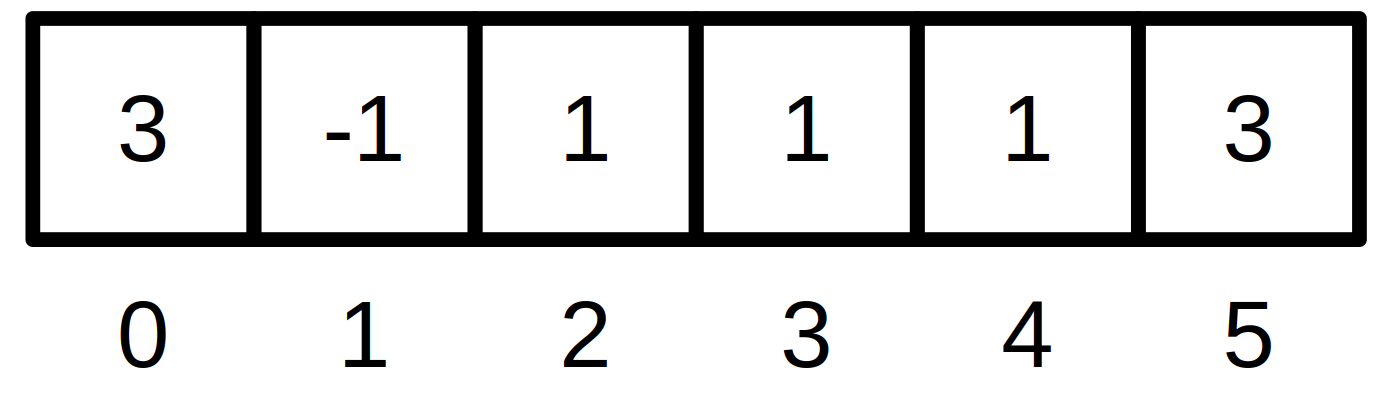
\includegraphics[width=0.9\linewidth]{lecon/10-arbres/arbre-tableau.png}
	\end{minipage}
\end{example}

\begin{rem}
	On ne stocke ici que la structure. Pour stocker des données, on produit un tableau de couples.
\end{rem}

\subsection{Représentation d'un arbre binaire presque complet}

\begin{definition}[Arbre binaire presque complet] \enspace\\
	\begin{minipage}{0.6\linewidth}
		Un arbre binaire presque complet est un arbre binaire dont tous les étages sont remplies sauf éventuellement le dernier qui est alors rempli à gauche
	\end{minipage} \qquad \begin{minipage}{0.4\linewidth}
		\begin{tikzpicture}[-]
			\node[state, scale=0.3] (q0) {};
			\node[state, scale=0.3, below left = 0.25 cm and 0.8cm of q0] (q1) {};
			\node[state, scale=0.3, below right = 0.25 cm and 0.8cm of q0] (q2) {};
			\node[state, scale=0.3, below left = 0.25 cm and 0.4cm of q1] (q3) {};
			\node[state, scale=0.3, below right = 0.25 cm and 0.4cm of q1] (q4) {};
			\node[state, scale=0.3, below left = 0.25 cm and 0.4cm of q2] (q5) {};
			\node[state, scale=0.3, below right = 0.25 cm and 0.4cm of q2] (q6) {};
			\node[state, scale=0.3, below left = 0.25 cm and 0.1cm of q3] (q7) {};
			\node[state, scale=0.3, below right = 0.25 cm and 0.1cm of q3] (q8) {};
			\node[state, scale=0.3, below left = 0.25 cm and 0.1cm of q4] (q9) {};
			
			\draw (q0) edge[] (q1);
			\draw (q0) edge[] (q2);
			\draw (q1) edge[] (q3);
			\draw (q1) edge[] (q4);
			\draw (q2) edge[] (q5);
			\draw (q2) edge[] (q6);
			\draw (q3) edge[] (q7);
			\draw (q3) edge[] (q8);
			\draw (q4) edge[] (q9);
		\end{tikzpicture}
	\end{minipage}
\end{definition}

\begin{minipage}{0.45\linewidth}
	\begin{principe}
		On peut alors représenter un tas par un tableau. On numérote alors les sommets ci contre, donnant l'indice dans le tableau. Les fils du noeuds d'indice $i$ se retrouve aux cases $2\times i+1$, $2\times i+2$, et son père $\left\lfloor \dfrac{i-1}{2}\right\rfloor$
	\end{principe}
\end{minipage}
\qquad
\begin{minipage}{0.45\linewidth}
	\begin{tikzpicture}[-]
		\node[state, scale=0.4] (q0) {};
		\node[state, scale=0.4, below left = 0.55 cm and 1.1cm of q0] (q1) {};
		\node[state, scale=0.4, below right = 0.55 cm and 1.1cm of q0] (q2) {};
		\node[state, scale=0.4, below left = 0.55 cm and 0.6cm of q1] (q3) {};
		\node[state, scale=0.4, below right = 0.55 cm and 0.6cm of q1] (q4) {};
		\node[state, scale=0.4, below left = 0.55 cm and 0.6cm of q2] (q5) {};
		\node[state, scale=0.4, below right = 0.55 cm and 0.6cm of q2] (q6) {};
		\node[state, scale=0.4, below left = 0.55 cm and 0.2cm of q3] (q7) {};
		\node[state, scale=0.4, below right = 0.55 cm and 0.2cm of q3] (q8) {};
		\node[state, scale=0.4, below left = 0.55 cm and 0.2cm of q4] (q9) {};
		
		\node[above right = 0cm and 0cm of q0] (l0) {\textcolor{cyan}{0}};
		\node[above left = 0cm and 0cm of q1] (l1) {\textcolor{cyan}{1}};
		\node[above right = 0cm and 0cm of q2] (l2) {\textcolor{cyan}{2}};
		\node[above left = 0cm and 0cm of q3] (l3) {\textcolor{cyan}{3}};
		\node[above right = 0cm and 0cm of q4] (l4) {\textcolor{cyan}{4}};
		\node[below = 0cm of q5] (l5) {\textcolor{cyan}{5}};
		\node[above right = 0cm and 0cm of q6] (l6) {\textcolor{cyan}{6}};
		\node[below = 0cm of q7] (l7) {\textcolor{cyan}{7}};
		\node[below = 0cm of q8] (l8) {\textcolor{cyan}{8}};
		\node[below = 0cm of q9] (l9) {\textcolor{cyan}{9}};
		
		\draw (q0) edge[] (q1);
		\draw (q0) edge[] (q2);
		\draw (q1) edge[] (q3);
		\draw (q1) edge[] (q4);
		\draw (q2) edge[] (q5);
		\draw (q2) edge[] (q6);
		\draw (q3) edge[] (q7);
		\draw (q3) edge[] (q8);
		\draw (q4) edge[] (q9);
	\end{tikzpicture}
\end{minipage}\\

\begin{example}\enspace\\
	\begin{minipage}{0.5\linewidth}
		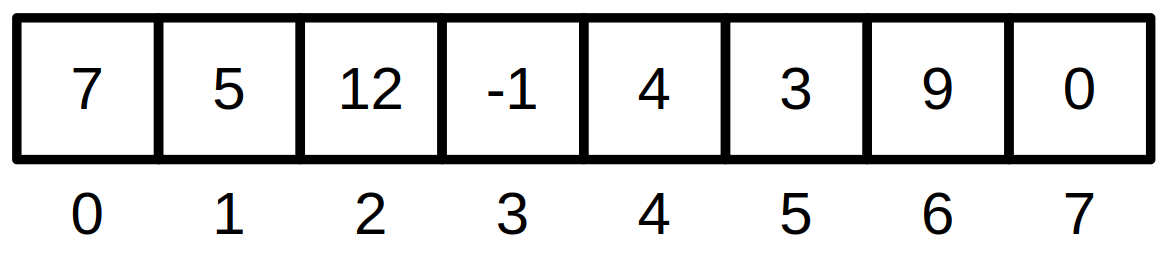
\includegraphics[width=\linewidth]{lecon/10-arbres/semi-complet.png}
	\end{minipage} \qquad
	\begin{minipage}{0.5\linewidth}
		\begin{tikzpicture}[-]
			\node[state] (q0) {7};
			\node[state, below left = 0.55 cm and 1.1cm of q0] (q1) {5};
			\node[state, below right = 0.55 cm and 1.1cm of q0] (q2) {12};
			\node[state, below left = 0.55 cm and 0.4cm of q1] (q3) {-1};
			\node[state, below right = 0.55 cm and 0.4cm of q1] (q4) {4};
			\node[state, below left = 0.55 cm and 0.4cm of q2] (q5) {3};
			\node[state, below right = 0.55 cm and 0.4cm of q2] (q6) {9};
			\node[state, below left = 0.55 cm and 0.2cm of q3] (q7) {0};
			
			\node[above right = 0cm and 0cm of q0] (l0) {\textcolor{cyan}{0}};
			\node[above left = 0cm and 0cm of q1] (l1) {\textcolor{cyan}{1}};
			\node[above right = 0cm and 0cm of q2] (l2) {\textcolor{cyan}{2}};
			\node[above left = 0cm and 0cm of q3] (l3) {\textcolor{cyan}{3}};
			\node[above right = 0cm and 0cm of q4] (l4) {\textcolor{cyan}{4}};
			\node[below = 0cm of q5] (l5) {\textcolor{cyan}{5}};
			\node[above right = 0cm and 0cm of q6] (l6) {\textcolor{cyan}{6}};
			\node[below = 0cm of q7] (l7) {\textcolor{cyan}{7}};
			
			\draw (q0) edge[] (q1);
			\draw (q0) edge[] (q2);
			\draw (q1) edge[] (q3);
			\draw (q1) edge[] (q4);
			\draw (q2) edge[] (q5);
			\draw (q2) edge[] (q6);
		\draw (q3) edge[] (q7);
		\end{tikzpicture}
	\end{minipage}
\end{example}

\section{Application}

\begin{com}
	A chaque fois on va écrire en début quelle représentation on utilise pour notre application. Néanmoins, en classe, on pourrait le laisser proposer par les élèves (une fois l'application présentée). On justifie de ce fait notre organisation, ou les applications arrivent toutes ensembles à la fin. (mais on écrit quand même la représentation au début pour que ce soit plus facile de naviguer à la partie que l'on souhaite).
\end{com}

\subsection{Dictionnaires}

\noindent \textbf{Représentation :} Structure inductive

\begin{definition}
	Un arbre binaire de recherche $N(x, G, D)$ est un arbre binaire de recherche (ABR) si $G$ et $D$ sont des ABR et si, selon un attribut $a$, $\max\limits_{u\in G} u.a\leq x.a \leq \min\limits_{v\in D} v.a$ (avec $E$ qui est un ABR et $\max\limits_{u\in E} u.a = -\infty$ et $\min\limits_{u \in E} u.a = +\infty$)
\end{definition}

\begin{proposition}
	Chercher et insérer dans un ABR est en $O(h)$
\end{proposition}

\begin{proposition}
	En imposant des contraintes supplémentaires (exemple arbres rouge-noir), on peut forcer $h = O(\log n)$
\end{proposition}

\begin{definition}
	Un dictionnaire (ou tableau associatif) est un tableau où les indices (clés) ne se limite pas à $\llbracket 0, n\rrbracket$
\end{definition}

\begin{idee}
	On peut alors implémenter un dictionnaire par un ABR, les clés étant les étiquettes des nœuds, à condition d'avoir un ordre total sur les clés
\end{idee}

\begin{theorem}
	Une implémentation efficace des dictionnaires par ABR permet des opérations de base en $O(\log n)$
\end{theorem}

\begin{com}
	Si on ne veut pas faire le développement 2, et qu'on préfère celui sur les arbres k-dimensionnel, on peut aussi parler aussi du pb des k-plus proches voisins et parler des ABR comme des arbres k-dim pour résoudre le pb
\end{com}

\subsection{Classes d'équivalence}

\noindent \textbf{Représentation :} Tableaux

\begin{definition}
	Une structure union \& trouver est une structure implémentant les classes d'équivalence, permettant de trouver les représentants d'une classe et d'unir deux classes.
\end{definition}

\begin{idee}
	On implémente cette structure sous formes d'un ensemble d'arbres (forêt), où chaque arbre représente une classe et où la racine est le représentant de la classe
\end{idee}

\begin{example}
	La relation d'égalité modulo 3 sur $\llbracket 0, 7 \rrbracket$ peut être représenté par : \\
	\begin{minipage}{0.4\linewidth}
		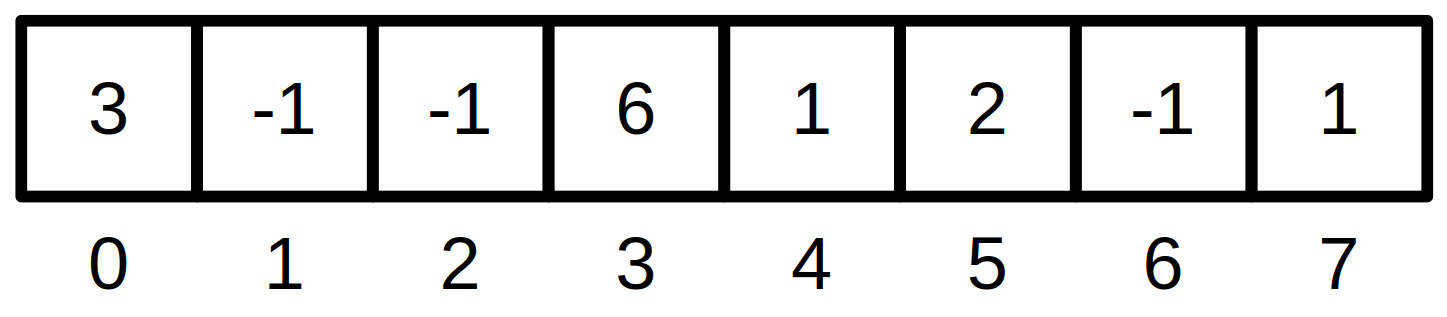
\includegraphics[width=\linewidth]{lecon/10-arbres/classe_equiv.png}
	\end{minipage}
	\qquad
 	\begin{minipage}{0.4\linewidth}
 		\begin{tikzpicture}[->, node distance=2cm]
 			\node[state] (q0) {$1$};
 			\node[state, below left of = q0] (q1) {$4$};
 			\node[state, below right of = q0] (q2) {$7$};	
 			\node[state, right = 2.5cm of q0] (q3) {$2$};
 			\node[state, below of = q3] (q4) {$5$};
 			\node[state, above right = 0.2cm and 2cm of q3] (q5) {$6$};
 			\node[state, below of = q5] (q6) {$3$};
 			\node[state, below of = q6] (q7) {$0$};
 			
 			\draw (q0) edge[] (q1);
 			\draw (q0) edge[] (q2);
 			\draw (q3) edge[] (q4);
 			\draw (q5) edge[] (q6);
 			\draw (q6) edge[] (q7);
 		\end{tikzpicture}
 	\end{minipage}
\end{example}

\begin{proposition}
	Si on unifie en faisant pointer la racine de l'arbre le moins profond vers celle de l'arbre le plus profond, on obtient des opérations unir et trouver en $O(\log(n))$
\end{proposition}

\subsection{Arbres couvrant de poids minimal}

\noindent \textbf{Représentation :} liste des arêtes

\begin{definition}
	Dans un graphe pondéré connexe, un arbre couvrant de poids minimal, est un sous-ensemble maximal d'arêtes sans cycles de somme de poids minimal.
\end{definition}

\begin{algorithm}[H]
	\caption{$Kruskal(L)$}
	\Entree{$L$ liste des arêtes}
	\Sortie{Liste des arêtes d'un ACM}
	$L\gets L$ trié\\
	$res \gets []$\\
	\Pour{$a$ parcourant $L$}
	{
		\Si{$a$ ne rajoute pas de cycle dans $res$}
		{
			Ajouter $a$ à $res$
		}
	}
	\Retour{$res$}
\end{algorithm}

\begin{proposition}
	En implémentant la détection de cycle par une structure union \& trouver, Kruskal renvoie un arbre couvrant de poids minimal en $O(|L| \times \log |L|)$
\end{proposition}

\subsection{Files de priorité}

\noindent \textbf{Représentation :} celles des arbres semi-complet

\begin{definition}
	Une file de priorité est une séquence de données dont on peut extraire la donnée d'attribut minimum, et rajouter des données.
\end{definition}

\begin{idee}
	On peut implémenter les files de priorité par des tas min
\end{idee}

\begin{definition}
	Un tas min est un arbre semi-complet où chaque noeud a un attribut plus petit que ses fils
\end{definition}

\noindent \textbf{Développement 2 :} Correction de l'insertion dans un tas min et discussion sur l'implémentation

\begin{principe}
	\enspace
	\begin{itemize}[label=$\star$]
		\item Pour ajouter un élément, on le met au bout du tablea et on l'échange avec son père tant qu'il est plus petit
		\item, Pour extraire le min, on met le dernier élément du tableau au début et on l'inverse avec le plus petit de ses fils tant qu'il est plus grand.
	\end{itemize}
\end{principe}

\begin{proposition}
	Cette implémentation permet des opérations en $O(\log n)$
\end{proposition}

\begin{appl}
	Trier par tas en $O(n \log n)$
\end{appl}

\chapter{Exemples d'algorithmes d'approximation et d'algorithmes probabilistes}
\label{L11}
\dev{Emile Martinez}{}

Beaucoup de problèmes sont durs à résoudre. On cherchera alors à sacrifier un peu de la fiabilité du résultat pour gagner en complexité. Il y a deux manières de faire un tel compromis : \begin{itemize}
	\item utiliser des algorithmes probabilistes (pouvant prendre beaucoup de temps, ou renvoyer faux)
	\item n'utiliser des algorithmes ne fournissant que des solutions approchées.
\end{itemize}

\section{Algorithmes probabilistes}

\begin{definition}
	Un algorithme est déterministe si, pour une entrée x donnée, il s’exécute toujours de la même manière. En particulier, la sortie ne dépend que de l'entrée.
	
	Un algorithme probabiliste est un algorithme dont l'exécution dépend de son entrée x et de valeurs obtenues via un générateur de nombre (pseudo)-aléatoire.
\end{definition}

\begin{example}
	\label{11-prem-ex}
	\normalfont
	Recherche dans un tableau $T$ de booléens d'un indice $i$ tel que $T[i] == True$\\
	\begin{minipage}{0.45\linewidth}
		\begin{algorithm}[H]
			\caption{$deterministe(T)$}
			\Pour{$i$ de $1$ à $|T|$}{
				\Si{$T[i]$}
				{
					\Retour{True}
				}
			}
			\Retour{False}
		\end{algorithm}
	\end{minipage} \qquad
	\begin{minipage}{0.45\linewidth}
		\begin{algorithm}[H]
			\caption{$probabiliste(T, k)$}
			\Pour{$j$ de $1$ à $k$}{
				Tirer uniformément $i$ dans $\llbracket 1, n \rrbracket$\\
				\Si{$T[i]$}
				{
					\Retour{True}
				}
			}
			\Retour{False}
		\end{algorithm}
	\end{minipage}
\end{example}

\begin{rem}
	Soit $p<1$ la proportion de booléen à Faux dans $T$. Alors l'algo probabiliste se trompe avec une probabilité = $p^k$.	
	Pour $p = \frac{1}{4}$ et $k=5$, cela fait $10^{-3}$
\end{rem}

\subsection{Algorithme de type Monte-Carlo}

\begin{definition}
	Un algorithme probabiliste A pour un pb P est de type Monte-Carlo si pour toute instance i de P, \begin{itemize}
		\item $A(i)$ est une solution, erronée avec une certaine probabilité
		\item Le temps d'exécution de $A$ sur $i$ est indépendant des choix aléatoires.
	\end{itemize} 
\end{definition}

\begin{example}
	L'algorithme probabiliste de l'exemple \ref{11-prem-ex} est de type Monte-Carlo
\end{example}

\textbf{Développement 1 :} Vérification probabiliste du produit matriciel

\begin{proposition}[Amplification]
    Soient $0 < \varepsilon_2 < \varepsilon_1 < 1$.
    
	S’il existe un algorithme Monte Carlo pour un problème $\Pi$ ayant une probabilité d’erreur $\varepsilon_1$, alors on peut construire un algorithme Monte Carlo pour le problème $\Pi$ ayant une probabilité d’erreur $\varepsilon_2$, en appliquant plusieurs fois l'algorithme initial.
\end{proposition}

\begin{algorithm}[H]
	\label{11-mediane}
	\caption{$mediane(L)$}
	$n \gets |L|$\\
	$L_{0} \gets k = n^{\frac{3}{4}}$ éléments de $L$ aléatoirement\\
	Trier $L_0$\\
	$x_1 \gets L_0[\frac{k}{2} - \sqrt{n}]$\\
	$x_2 \gets L_0[\frac{k}{2} + \sqrt{n}]$\\
%	$L_1, \, L_2, \, L_3 \gets[], \, [], \, []$\\
%	\Pour{$x \in L$}
%	{
%		\eSi{$x \leq x_1$}
%		{
%			Ajouter $x_1$ à $L_1$
%		}{
%		\eSi{$x \leq x_2$}
%		{
%			Ajouter $x$ à $L_2$
%		}
%		{
%			Ajouter $x$ à $L_3$
%		}
%		}
%	}
	$L_1 \gets $ liste des éléments $< x_1$\\
	$L_2 \gets$ liste des éléments entre $x_1$ et $x_2$\\
	$L_3 \gets$ liste des éléments $> x_2$\\
	\Si{$|L_1| > \frac{n}{2}$ ou $|L_3| > \frac{n}{2}$}{\Retour{n'importe quoi}\tcp*{$L_2$ n'a pas capturé la médiane}}
	\Si{$|L_2| > n^{\frac{3}{4}}$}{\Retour{n'importe quoi}\tcp*{On a trop d'éléments dans $L_2$ pour les trier}}
	Trier $L_2$\\
	\Retour{$L_2[\frac{n}{2} - |L_1|]$}
\end{algorithm}

\begin{idee}
	On fait la médiane sur un échantillon de $L$. Puis on prend tous les éléments autour de cette médiane et on les trie pour trouver la vraie médiane (si elle y est, sinon tant pis).
\end{idee}

\begin{com}
	Ici le temps dépend du hasard. On considère quand même que c'est un Monte Carlo car c'est borné et prend le temps moyen est un $\Omega$ du temps dans le pire des cas. On pourrait aussi a la place de retourner n'importe quoi, trier $n^{3/4}$ éléments et remplir $L_2$ avec des $= \infty$ mais alors on complexifie pour rien.
\end{com}

\subsection{Algorithmes de type Las Vegas}

\begin{definition} 
	Un algorithme probabiliste $A$ est de Las Vegas si :
	\begin{itemize}
		\item Si $A$ termine, alors la solution renvoyée est correcte.
		\item Le temps d'exécution de $A$ est une variable aléatoire.
	\end{itemize}
\end{definition}

\begin{rem}
	Quand on parle de complexité en moyenne pour un algorithme de Las Vegas, on ne considère pas (ou pas uniquement) la moyenne des complexité sur toutes les entrées possibles prisent uniformément, mais la plus grande espérance du temps d'exécution sur une entrée
\end{rem}


\begin{algo}
	\normalfont \enspace\\
	\label{11-tri-rapide}
	\begin{algorithm}[H]
		\caption{$tri\_rapide\_randomise(T)$}
		\Si{$|T| = 1$}{\Retour}
		Tirer $q$ uniformément dans $\llbracket 1, |T| \rrbracket$ \tcp*{$T[q]$ sera le pivot}
		$i \gets partition(T, q)$\\
		$tri\_rapide\_randomise(T[:i])$\\
		$tri\_rapide\_randomise(T[i+1:])$\\
	\end{algorithm}
	où $partition(T, q)$ mets dans $T$, tous les éléments $< T[q]$ puis tous les éléments supérieurs, et renvoie l'indice du milieu.
\end{algo}

\begin{rem}
	Le temps d'exécution de l'algorithme \ref{11-tri-rapide} dépend du choix du pivot : $O(n^2)$ dans le pire cas, $O(n\log n)$ dans le meilleur et en moyenne. 
\end{rem}

\begin{rem}
	Il est possible de transformer un algorithme de type Las Vegas en Monte Carlo en l'exécutant pendant un temps défini et en générant une réponse aléatoire s'il n'a pas terminé.
\end{rem}

\begin{rem}
	Si on peut vérifier efficacement la validité du résultat, on peut également faire l'inverse.
\end{rem}

\begin{example}
	A la place de l'échec dans l'algorithme \ref{11-mediane}, on peut relancer l'algorithme. On obtient alors un algorithme trouvant toujours la médiane, la calculant en moyenne en $1,5n$ comparaisons, sans adversaires, ce qui est mieux que tout algorithme déterministe (qui ont nécessairement besoin d'au moins $2n$ comparaisons en moyenne).
\end{example}

\section{Algorithmes d'approximation}

\subsection{Définition}


\begin{definition}
	Un problème d’optimisation est un problème $\Pi = (I, S, c)$ où \begin{itemize}
		\item $I$ est l'ensemble des instances
		\item $\forall i \in I, S(i)$ est l'ensemble des solutions pour $i$
		\item $c : I \times S \to R$ fonction d'évaluation.
	\end{itemize}
	Étant donnée une instance $i \in I$, l’objectif est de construire une solution $s^{*} \in S(i)$ vérifiant : $c(i, s^{*}) = \min\left\{c(x, s) \big/ s \in S(i)\right\}$
\end{definition}

\begin{com}
	On peut aussi demander à ce que $c$ soit calculable en temps polynomial mais ce n'est pas nécessaire. Les deux définitions coexistent.
\end{com}

\begin{rem}
	On se ramène au max en prenant $-c$.
\end{rem}

\begin{definition}
	    Une $\lambda$-approximation est un algorithme polynomial $A$ donnant pour chaque instance $i$ de $\Pi$ une solution tel que $\max\left(\left| \dfrac{A(i)}{OPT(i)} \right|, \left| \dfrac{OPT(i)}{A(i)} \right|\right) \leq \lambda$
\end{definition}

\subsection{Exemples}

\begin{definition}[Couvertue par des sommets (Vertex-Cover)]
	Entrée : Un graphe $G = (S, A)$
	Solution : Un ensemble $S \subset V$ tel que $\forall u, v \in E, \,v\in S \text{ ou } u \in S$
\end{definition}

\begin{algorithm}[H]
	\label{11-glouton-vc}
	\caption{Glouton Vertex Cover}
	$S \gets \{\}$\\
	\Tq{il existe une arête $(u,v) \in A$ tel que $u\notin S$ et $v \notin S$}
	{
		Choisir $(u,v)$ une telle arête\\
		$S \gets S \cup \{(u,v)\}$
	}
	\Retour{$S$}
\end{algorithm}

\begin{proposition}
	L'algorithme \ref{11-glouton-vc} est une 2-approx du problème de la couverture par les sommets.
\end{proposition}



\noindent \textbf{Développement :} Une $\frac{3}{2}$-approximation et une $\frac{7}{6}$-approximation gloutonnes pour le problème d'ordonnancement de tâches indépendantes sur 2 processeurs.



\begin{definition}[Voyageur de commerce (TSP)]
	Instance : $G = (S, A, c)$ un graphe orienté complet pondéré\\
	Solution : Un cycle hamiltonien sur $G$ de poids minimal
\end{definition}

\begin{theorem}
	Il n'existe pas d'algorithme d'approximation pour TSP, sauf si $P = NP$.
\end{theorem}

\begin{algo}[Algorithme pour TSP]
	\label{11-approx-tsp}
	\enspace \begin{enumerate}
		\item $\mathcal A \gets$ arbre couvrant de poids minimal de $G$
		\item $P \gets$ parcours en profondeur préfixe de $\mathcal A$
		\item Renvoyer $P$
	\end{enumerate}
\end{algo}

\begin{proposition}
	L'algorithme \ref{11-approx-tsp} est une 2-approx si $c$ vérifie l'inégalité triangulaire ($\forall x, y, z\in C, \, c(x, y) + c(y, z) \geq c(x, z)$)
\end{proposition}

\begin{example} \normalfont \enspace \\
	\begin{tikzpicture}[-]
		%etape 1
		\node[state, scale=0.4] (a0) {};
		\node[state, scale=0.4, below left = 1cm and 0.75cm of a0] (a1) {};
		\node[state, scale=0.4, below right = 1cm and 0.75cm of a0] (a2) {};
		\node[state, scale=0.4, above right = 0.4cm and 1.2cm of a0] (a3) {};
		\node[state, scale=0.4, above = 1.2cm of a0] (a4) {};
		\node[state, scale=0.4, above left = 0.4cm and 1.2cm of a0] (a5) {};
		
		\draw (a0) edge[green] (a1);
		\draw (a0) edge[green] (a2);
		\draw (a0) edge[green] (a3);
		\draw (a0) edge[green] (a4);
		\draw (a0) edge[green] (a5);
		
		\draw (a1) edge[black] (a2);
		\draw (a2) edge[black] (a3);
		\draw (a3) edge[black] (a4);
		\draw (a4) edge[black] (a5);
		\draw (a5) edge[black] (a1);
		
		\draw (a1) edge[red] (a3);
		\draw (a2) edge[red] (a4);
		\draw (a3) edge[red] (a5);
		\draw (a4) edge[red] (a1);
		\draw (a5) edge[red] (a2);
		
		%légende
		\node[below left = 1cm and 0cm of a1] (l1) {};
		\node[right = 0.5cm of l1] (l2) {};
		\node[right = 0cm of l2] {coût 1};
		\node[below = 0.2cm of l1] (l3) {};
		\node[right = 0.5cm of l3] (l4) {};
		\node[right = 0cm of l4] {coût 1};
		\node[below = 0.2cm of l3] (l5) {};
		\node[right = 0.5cm of l5] (l6) {};
		\node[right = 0cm of l6] {coût 2};
		
		\draw (l1) edge[red] (l2);
		\draw (l3) edge[green] (l4);
		\draw (l5) edge[black] (l6);
		
		%flèche 1
		\node[below right = 0.9cm and 1.4cm of a0] (f1) {};
		\node[below right = 0.6cm and 0.9cm of f1] (f2) {};
		
		\draw (f1) edge[->, above right] node{1} (f2);
		
		%etape 2
		\node[state, scale=0.4, label = {[yshift=-1cm]A}, below right = 1.1cm and 1.6 cm of f2] (b0) {};
		\node[state, scale=0.4, label = B, below left = 1cm and 0.75cm of b0] (b1) {};
		\node[state, scale=0.4, label = C, below right = 1cm and 0.75cm of b0] (b2) {};
		\node[state, scale=0.4, label = D, above right = 0.4cm and 1.2cm of b0] (b3) {};
		\node[state, scale=0.4, label = E, above = 1.2cm of b0] (b4) {};
		\node[state, scale=0.4, label = F, above left = 0.4cm and 1.2cm of b0] (b5) {};
		
		\draw (b0) edge[green] (b1);
		\draw (b0) edge[green] (b2);
		\draw (b0) edge[green] (b3);
		\draw (b0) edge[green] (b4);
		\draw (b0) edge[green] (b5);
		
		%flèche 2
		\node[above = 0.7cm of b4] (f3) {};
		\node[above = 0.9cm of f3] (f4) {};
		
		\draw (f3) edge[->, right] node{2} (f4);
		
		%etape 3
		\node[above = 0cm of f4] (c0) {ABCDEFA};
		
		%flèche 3
		\node[below right = 0cm and 0.5cm of c0] (f5) {};
		\node[below right = 0.6cm and 2cm of f5] (f6) {};
		
		\draw (f5) edge[->, above right] node{3} (f6);
		
		%etape 4
		\node[state, scale=0.4, below right = 1cm and 1.8cm of f6] (d0) {};
		\node[state, scale=0.4, below left = 1cm and 0.75cm of d0] (d1) {};
		\node[state, scale=0.4, below right = 1cm and 0.75cm of d0] (d2) {};
		\node[state, scale=0.4, above right = 0.4cm and 1.2cm of d0] (d3) {};
		\node[state, scale=0.4, above = 1.2cm of d0] (d4) {};
		\node[state, scale=0.4, above left = 0.4cm and 1.2cm of d0] (d5) {};
		
		\draw (d0) edge[green] (d1);
		\draw (d1) edge[black] (d2);
		\draw (d2) edge[black] (d3);
		\draw (d3) edge[black] (d4);
		\draw (d4) edge[black] (d5);
		\draw (d5) edge[green] (d0);
		
		%conclusion
		\node[below = 1.5cm of d0] {On a un coût de 10 et non de 6};
		
	\end{tikzpicture}
\end{example}

\section{Algorithmes d'approximation probabilistes}

Il existe des algorithmes d'approximation probabilistes. Ce sont alors souvent des algorithmes de Monte Carlo.

\subsection{Max Sat}

\begin{definition}
	Instance : $n$ variables $\{x_1, \dots, x_n\}$, p clauses $C_1, \dots, C_p$ sur $(x_1, \dots, x_n$) contenant au moins k littéraux
	Solution : Trouver une valuation maximisant le nombre de clauses à vrai
\end{definition}

\begin{example}
	Si $\varphi = \bigwedge\limits_{i=1}^p C_i$ est satisfiable, une solution optimale est une valuation satisfaisant $\varphi$
\end{example}

\begin{algo}
	Renvoyer une valuation aléatoire.
\end{algo}

\begin{theorem}
	L'espérance du nombre de clauses satisfaites $\mathbb E(\varphi)$ vérifie $\mathbb E(\varphi) \geq p\left( 1 - \dfrac{1}{2^k}\right) \geq \dfrac{c}{2}$
\end{theorem}

\begin{rem}
	On peut créer un algorithme déterministe qui est une $\left( 1 - \dfrac{1}{2^k} \right)$-approx.
\end{rem}

\subsection{Calcul de $\pi$}

On peut calculer une valeur approchée de $\pi$ par des méthodes probabilistes

\begin{algorithm}
	\caption{$calcul\_pi(N)$}
	$i \gets O$\\
	\Repeter{$N$ fois}
	{
		Tirer deux flottants $x, y$ dans $[-1, 1]$ uniformément\\
		\Si{$x^2+y^2 < 1$ }
		{
			$i \gets i+1$ \tcp*{On a tapé dans le cercle d'aire $\pi$}
		}
	}
	\Retour $\dfrac{4i}{N}$\tcp*{Nombre de points dans le cercle / aire du carré = $\frac{\pi}{4}$}
\end{algorithm}

\begin{com}
	On peut aussi mettre un dessin ici pour expliquer ce qui se passe.
\end{com}

\begin{com}
	Si on veut parler plus précisément d'algorithme d'approximation, on prendrait dans la def, pour $I$ la manière de représenter les flottants (nb de bits d'exposant, de mentisse, etc\dots) et pour $S$ de tels flottants. La fonction de coût $c$ serait alors la distance à $pi$ (même si pas facilement calculable en temps polynomial)
\end{com}

\begin{rem}
	On peut généraliser la méthode pour le calcul d'intégrales
\end{rem}

\begin{rem}
	Cette méthode se généralise en une méthode de Monte Carlo où l'on échantillone le problème, on calcule la solution sur cette échantillon, puis on généralise la solution à partir de cet échantillon.
\end{rem}

\chapter{Exemples d'algorithmes glouton et de retour sur trace}
\label{L12}
\dev{Emile Martinez}{}

Quand on aborde un problème à la main, on essaye souvent de construire des solutions au fur et à mesure, en faisant plein de choix locaux. Essayons de mettre cela en oeuvre algorithmiquement.

\section{Algorithmes gloutons}

\subsection{Définition}

\begin{definition}
	Un algorithme glouton construit une solution à un problème par choix successifs considérés localement optimaux, sans jamais revenir en arrière.
\end{definition}

\textbf{Avantage :} C'est souvent peu coûteux, et potentiellement en ligne.

\begin{example}[Gymnases]\enspace
	\begin{itemize}
		\item[Instances :] $n$ évènements, leur date de début $\left\{d_i\right\}_{i \in \{1, \dots, n\}}$ et de fin $\left\{f_i\right\}_{i \in \{1, \dots, n\}}$
		\item[Problème :] trouver un nombre minimal de gymnases pour organiser les évènements
	\end{itemize}
\end{example}

\begin{algo}\enspace
	\begin{enumerate}
		\item Trier les évènements par dates de début croissantes
		\item Allouer successivement le premier gymnase disponible. En ouvrir un si nécessaire.
	\end{enumerate}
\end{algo}

\chapter{Exemples d’algorithmes utilisant la méthode « diviser pour régner »}
\label{L13}
\dev{Emile Martinez}{}

\section{Introduction}

\begin{definition}[Paradigme Diviser pour Régner]Un algorithme de type Diviser pour Régner s'effectue en 3 étapes : \begin{enumerate}
		\item Division du problème en sous-problèmes indépendants
		\item Résolution récursive des sous-problèmes
		\item Construction d'une solution du problème global à partir des solutions des sous-problèmes
\end{enumerate}
	
\end{definition}

\begin{principe}[Calcul de la compléxité d'un tel algorithme.]
	
	Trouver une fonction donnant la taille du problème (comme le nombre d'éléments pour une liste). Définir $C$ la complexité maximale des instances de cette taille, puis trouver une relation de réccurence sur $C$, pour tenter de la résoudre.
	
\end{principe}

\begin{com}
	La méthode de résolution sera inculqué par l'exemple, et progressivement (d'abord le cas de base, où l'on découpe en seulement 2 avec l'exponentiation rapide, puis on complexifie)
\end{com}

\section{Applications au calcul formel}

\subsection{L'exponentiation rapide}

\textbf{Problème :} Étant donné un entier $a$ et un entier positif $n$, calculer $a^n$.

\textbf{Solution naïve :} $n$ multiplications

\begin{algo}[Méthode D\&R] \enspace \\
	\begin{minipage}{0.7\linewidth}
		\begin{algorithm}[H]
			\caption{$exponentiation\_rapide(a, n)$}
			\Si{$n = 0$}
				{\Retour{$1$}}
			$m \gets m/2$ \tcp*{étape 1}
			$x \gets exponentiation\_rapide(a, m)$ \tcp*{étape 2}
			\eSi(\tcp*{étape 3}){$n$ est pair}
				{\Retour{$x\times x$}}
				{\Retour{$x\times x \times a$}}
		\end{algorithm}
	\end{minipage}
\end{algo}

\begin{proposition}[Complexité]
	La complexité en nombre de multiplication par rapport à l'entier positif (noté $C(n)$) vaut $C(n) = O\big(\log(n)\big)$
\end{proposition}

\begin{proof}
	\label{13-preuve}
	\begin{enumerate}
		\item $C(n) = C\left(\left\lfloor\dfrac{n}{2}\right\rfloor \right) + O(1)$
		\item $C$ est majoré par $D(n) = D\left(\left\lfloor\dfrac{n}{2}\right\rfloor\right) + K$
		\item $D$ est croissante
		\item $D\left(2^k\right)$ est une suite arithmétique donc $D\left(2^k\right) = O(k)$
		\item $C(n) \underset{\substack{\uparrow\\2}}\leq D(n) \underset{\substack{\uparrow\\3}}\leq D\left(2^{\left\lfloor\log(n)\right\rfloor+1}\right) \underset{\substack{\uparrow\\4}}= O(\log(n))$
	\end{enumerate}
\end{proof}

\subsection{Multiplication matricielle}

\textbf{Problème :} Étant donné $A = (a_{i,j})$ et B = $(b_{i,j})$ deux matrices de taille $n$, on cherche à calculer $A_\times B$

\textbf{Solution naïve :} $O(n^3)$
\begin{algo}[Méthode D\&R : Algorithme de Strassen]
	\begin{enumerate}
		\item Rajouter des 0 pour que $A$ et $B$ soient de tailles paires. Diviser alors $A$ et $B$ en matrices de taille $\frac{n}{2}$
		$$A = \left( \begin{array}{c|c}
			A_{1, 1} & A_{1, 2} \\ \hline
			A_{2, 1} & A_{2, 2}
		\end{array}\right) \text{ et } B = \left( \begin{array}{c|c}
		B_{1, 1} & B_{1, 2} \\ \hline
		B_{2, 1} & B_{2, 2}
		\end{array}\right)$$
		
		\item Calculer récursivement \\
		$M_1 = (A_{1, 1} + A_{2, 2}) \times (B_{1, 1} + B_{2, 2}) $\\
		$M_2 = (A_{2, 1} + A_{2,2}) \times B_{1, 1} $\\
		$M_3 = A_{1, 1} \times (B_{1, 2} - B_{2, 1})$\\
		$M_4 = A_{2, 2} \times (B_{2, 1} - B_{1, 1})$\\
		$M_5 = (A_{1, 1} + A_{1, 2}) \times B_{2, 2}$\\
		$M_6 = (A_{2, 1} - A_{1, 1}) \times (B_{1, 1} + B_{1, 2})$\\
		$M_7 = (A_{1, 2} - A_{2, 2}) \times (B_{2, 1} + B_{2, 2})$\\
		
		\item Calculer $A\times B = \left( \begin{array}{c|c}
			M_1 + M_4 - M_5 + M_7 & M_3 + M_5 \\ \hline
			M_2 + M_4 & M_1 - M_2 + M_3 + M_6
		\end{array}\right)$
		
	\end{enumerate}
\end{algo}

\begin{exercise}
	Prouver la correction de l'algorithme de Strassen.
\end{exercise}

\begin{proposition}
	Cette algorithme a une complexité en $O\left( n ^{\log_2(3)}\right)$
\end{proposition}

\begin{exercise}
	Prouver cela en reprenant la preuve pour l'exponentiation en considérant $\dfrac{D(2^k)}{7^k}$ à l'étape 4 de la preuve \ref{13-preuve}
\end{exercise}

\section{Application aux listes}
	
\subsection{Recherche dichotomique}

\label{13-dico}

\textbf{Problème :} Rechercher un élément $a$ dans une liste $L$ d'éléments triés selon un ordre $\leq$

\begin{algorithm}[H]
	\Entree{$L$ une liste triée, $a$ un élément}
	\Sortie{$i$ tel que $L[i] = a$ s'il existe, $-1$ sinon}
	\caption{$recherche\_dichotomique(l, a, debut, fin)$}
	\Si{$fin < debut$}
		{\Retour $-1$}
	$m \gets \left\lfloor \dfrac{debut + fin}{2}\right\rfloor$ \\
	\Si{$l[m] =- a$}
		{\Retour $m$}
	\eSi{$l[m] < a$}
		{\Retour{$recherche\_dichotomique(l, a, m+1, fin)$}}
		{\Retour{$recherche\_dichotomique(l, a, debut, m+1)$}}
\end{algorithm}

\begin{exercise}
	Ecrire le code en plus de lignes et faire apparaître les 3 étapes de D\&R
\end{exercise}

\begin{proposition}
	La recherche dichotomique est en $O(\log |L|)$
\end{proposition}

\begin{exercise}
	Écrire une version itérative de cet algorithme
\end{exercise}

\subsection{Tri fusion}
\label{13-tri-fusion}

\begin{algorithm}[H]
	\caption{$fusion(L_1, L_2)$}
	\Entree{$L_1$, $L_2$ deux listes triées d'éléments comparables}
	\Sortie{La fusion des listes $L_1$ et $L_2$ triée}
	$res \gets []$\\
	$i,j \gets 0$\\
	\Tq{
		$i < |L_1|$	et $j < |L_2|$
	}{
		\eSi{$L_1[i] < L_2[j]$}{
			$res$.ajouter($L_1[i]$) \\
			$i \gets i + 1$
		}{
			$res$.ajouter($L_2[j]$) \\
			$j \gets j + 1$
		}
	}
	Ajouter le reste de $L_1$ et de $L_2$ à $res$\\
	\Retour{$res$}
\end{algorithm}

\begin{algorithm}[H]
	\caption{$tri\_fusion(L)$}
	\Entree{Une liste $L$ d'éléments comparables}
	\Sortie{La liste $L$ triée}
	$n \gets |L|$\\
	\Si{$n\leq 1$}{
		\Retour{$L$}
	}
	$L_1, L_2 \gets partionner(L)$ \tcp*{Étape 1}
	$A \gets tri\_fusion(L_1)$ \tcp*{Étape 2}
	$B \gets tri\_fusion(L_2)$
	\Retour{$fusion(A, B)$}
\end{algorithm}

\begin{proposition}
	Le tri fusion est $O(n \log n)$ avec $n = |L|$
\end{proposition}

\begin{proof}
	Exercice
\end{proof}

\textbf{Développement :} Correction et terminaison du tri fusion

\begin{appl}
	Si l'on veut chercher si $K$ entiers sont présents parmi $N$, on peut avec \ref{13-dico} et \ref{13-tri-fusion} faire cela en $O\big((N + K) \log N \big)$ au lieu de $O(k\times N)$
\end{appl}



\subsection{Tri rapide}

\textbf{Objectif :} Faire un tri D\&R en place

\begin{com}
	Ici, on peut avoir des questions sur le tri fusion en place, ce qui existe plus ou moins mais est assez pénible. Donc ca peut valoir le coup de se renseigner sur le sujet.
\end{com}

\begin{idee}
	Choisir un élément appelé pivot et mettre à gauche tous les éléments plus petit, à droite tous les plus grands, puis à trier cette partie à droite et à gauche.
\end{idee}

\begin{algorithm}
	\caption{$tri\_rapide(L, debut, fin)$}
	\Si{$debut \geq fin -1$}
	{\Retour{$L$}}	
	$pivot \gets L[0]$\\	
	$i \gets debut$\\
	$j \gets fin$\\
	\Tq{$i < j$}
	{
		\eSi{$L[i+1] \leq pivot$}
		{
			échanger $L[i+1]$ et $L[i]$\\
			$i \gets i+1$
		}{		
			échanger $L[i+1]$ et $L[j]$\\
			$j \gets j - 1$
		}
		
		$tri\_rapide(L, debut, i-1)$\\	
		$tri\_rapide(L, i+1, fin)$\\
	}
\end{algorithm}

\begin{com}
	Par manque de place, on peut remplacer l'écriture de cet algorithme par un dessin expliquant l'idée, et mettre son écriture en exercice.
\end{com}

\begin{proposition}
	Ce tri est dans le pire des cas en $O(n^2)$, dans le cas moyen en $O(n \log n)$. Il est néanmoins en place (en autorisant un espace non pas constant mais logarithmique).
\end{proposition}

\begin{com}
	L'occasion de briller sur le fait que le tri rapide écrit comme ça n'est pas en place avec la définition première, mais l'est avec la définition élargie où on autorise $O(\log n)$ espace (utilisé par les appels récursifs)
\end{com}

\section{Application Géométrique}

\subsection{Plus petite distance dans le plan}

\textbf{Problème :} Étant donné $n$ points de $\mathbb R^2$, donner la plus petite distance entre deux points

\textbf{Solution naïve :} $n$ multiplications

\begin{algo}[Solution D\&R]
	\begin{enumerate}
		\item Choisir une abscisse $x_m$ séparant les points en deux sous-ensembles $P_1$ et $P_2$ de taille égale (à + ou - 1)
	
		\item Trouver les plus petites distances $d_1$ et $d_2$ de $P_1$ et $P_2$
	
		\item Rechercher la plus petite distance $d_3$ entre deux points dans la bande d’abscisse $[x_m-d_0, x_m+d_0]$ pour $d_0$ = $\min d_1, d_2$
	
	\end{enumerate}
\end{algo}

L'étape 3 peut se faire en ne regardant que les 7 points suivants (suivants au sens de l'ordonnée).\\
\begin{minipage}{0.35\linewidth}
	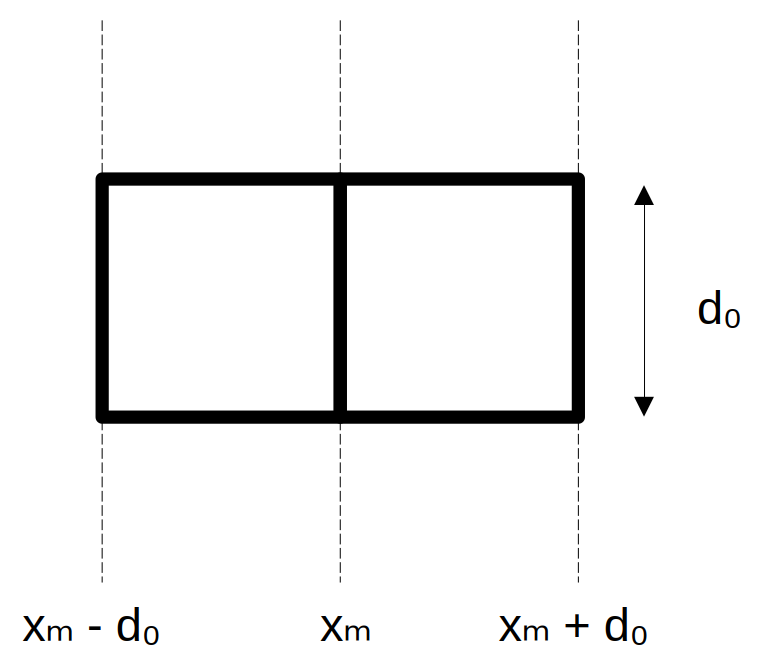
\includegraphics[width=\linewidth]{lecon/13-D&R/7_points.png}
\end{minipage}
\qquad
\begin{minipage}{0.5\linewidth}
	On a au plus 8 éléments dans ce rectangle, car dans chaque domaine, les points sont au moins à distance $d_0$. On a donc au plus $4$ points par carré, d'où le résultat en mettant notre point sur le bas du rectangle.
\end{minipage}

\begin{proposition}
	On a une complexité en $O\left(n (\log n)^2\right)$
\end{proposition}




\subsection{Arbre K-dimensionnel}

\textbf{Problème :} Trouver les $k$ plus proches voisins d'un point $y \in \mathbb R^K$ parmi un ensemble de $n$ points $x_1, \dots, x_n \in \mathbb R^K$

\textbf{Solution initiale :} Stocker nos $k$ valeurs en cours dans une file de priorité et parcourir les n points, en mettant à jour la file de priorité. $\to O(n \log k)$

\begin{algo}[Solution D\&R]
	Faire un pré traitement où l'on stockera nos valeurs dans un arbre binaire de recherche, où l'on partitionnera récursivement les données alternativement sur chaque dimension. La recherche se fait alors en ne cherchant que d'un côté si le deuxième n'est pas nécessaire.
\end{algo}

\textbf{Développement :} Présentation de la structure d'arbre K-dimensionnel

\begin{proposition}[Complexité]\enspace
	\begin{itemize}
		\item prétraitement : $O(n \log(n))$
		\item Recherche des $k$ plus proches voisins : $O(\log n \times k)$ en moyenne, $O(N \times K)$ dans le pire des cas
	\end{itemize}
\end{proposition}


\begin{rem}
	On y perd pour une seule recherche, mais si on cherche les $k$-plus proches voisins de $N$ points, on obtient du $O(n \log n + N \times k \times \log n)$ au lieu de $O(N \times n \times \log k)$.
\end{rem}

\begin{com}
	Si il reste beaucoup de places ou si on veut enlever un exemple au dessus (comme le tri rapide faisant doublons avec le tri fusion, même si il est très classique), on peut rajouter une section supplémentaire ici, et parler de l'additionneur à retenue anticipée par méthode D\&R du développement *à compléter*
\end{com}	

\chapter{Programmation dynamique} \label{L14}
\dev{Emile Martinez}{}

\begin{com}
	On présentera d'abord le principe de la méthode diviser pour régner. Ensuite on divise nos exemples, en deux : ceux qu'on verrait dans la leçon diviser pour régner car ils sont là spécifiquement pour illustrer le paradigme, et ceux que l'on verrait au cours de l'année, et s'appuyant sur le fait qu'on ait déjà vu la méthode diviser pour régner. Cette distinction vient du fait que dans un vrai cours, on ferait comme ça, et les problèmes de la dernière partie serait insérer dans autre chose, et on souligne alors le fait que on ne ferait pas simplement une liste d'algo, mais que pour que le paradigme soit assimiler, il faut mieux le présenter et y revenir régulièrement, plutôt que d'introduire plusieurs fois beaucoup de concepts. (et on met ainsi de la structure sans faire simplement une liste)
\end{com}

\section{Principe}

\subsection{Motivation}

\begin{algo}
	Implémentation naïve de la suite de Fibonacci\\
	\begin{algorithm}[H]
		\caption{$fibo(n)$}
		\eSi{$n = 0$ ou $n = 1$}
			{\Retour{$n$}}
			{\Retour{$fibo(n-1) + fibo(n-2)$}}
	\end{algorithm}
\end{algo}

\begin{proposition}
	Complexité en $O(2^n)$
\end{proposition}

Graphe des dépendances des sous problèmes pour $n = 5$

\begin{minipage}{0.3\linewidth}
	\begin{tikzpicture}[->, node distance=2cm]
		\node[state] (q0) {$F_5$};
		\node[state, below left of = q0] (q1) {$F_3$};
		\node[state, below right of =q0] (q2) {$F_4$};
		\node[state, below of =q1] (q3) {$F_1$};
		\node[state, below of =q2] (q4) {$F_2$};
		\node[state, below right of=q3] (q5) {$F_0$};
		
		\draw (q0) edge[] (q1);
		\draw (q0) edge[] (q2);
		\draw (q2) edge[] (q1);
		\draw (q1) edge[] (q3);
		\draw (q1) edge[] (q4);
		\draw (q2) edge[] (q4);
		\draw (q4) edge[] (q3);
		\draw (q4) edge[] (q5);
		
	\end{tikzpicture}
\end{minipage} \qquad
\begin{minipage}{0.6\linewidth}
	Les sous-problèmes se chevauchent : la méthode diviser pour régner est inefficace.\\\\
	En programmation dynamique, on stocke les valeurs des sous-problèmes pour éviter de recalculer.
\end{minipage}

\begin{algo}
	\label{14-fibo2}
	Fibonacci avec stockage.\\
	\begin{algorithm}[H]
		\caption{$Fibo(n)$}
		$F \gets [0, 1]$\\
		\Pour{$i$ allant de $2$ à $n$}
			{Ajouter $F[i-1] + F[i-2]$ à $F$}
		\Retour{$F[n]$}
	\end{algorithm}
\end{algo}

\subsection{Définition}

\begin{definition}
	La programmation dynamique consiste à résoudre un problème en le décomposant en sous-problèmes, puis à résoudre les sous-problèmes, des plus petits aux plus grands en stockant les résultats intermédiaires.
\end{definition}

\begin{principe}
	\enspace
	\begin{enumerate}
		\item Complexifier le problème en créant plein de sous-problèmes (dont un sera celui que l'on veut résoudre)
		\item Trouver une relation entre les sous-problèmes
		\item Résoudre les sous-problèmes en partant du plus petit, en utilisant la relation :\begin{itemize}
			\item Soit impérativement en ayant un tableau des sous-problème qui stockera leur résultat, et en le remplissant avec une (ou des) boucle (méthode ascendante)
			\item Soit récursivement en mémoïsant. (méthode descendante)
		\end{itemize}
		
	\end{enumerate}
\end{principe}

\begin{rem}
	L'algorithme \ref{14-fibo2} utilise la méthode ascendante. On aurait pu utiliser uniquement deux variables et écraser les résultats intermédiaires.
\end{rem}

\begin{rem}
	Dans le paradigme diviser pour régner, les sous pb sont indépendants. On peut donc se passer de la mémoïsation.
\end{rem}

\begin{rem}
	Pour obtenir, en plus de la valeur de la solution optimale, quelle est cette solution, on peut mémoriser quel(s) sous-problème(s) on a utilisé pour l'obtenir.
\end{rem}

\textbf{Développement :} Illustration du paradigme sur le problème du chemin dans la pyramide.

\section{Algorithmes illustrant le principe}

\subsection{Rendu de monnaie}

\textbf{Instance :} $n$ pièces $p_1, ... p_n$, $S \in \N$

\textbf{Pb :} trouver un $n$-uplet $T = (x_1,  \dots, x_n) \in \N^n$ te que $\sum\limits_{i = 1}^n x_i p_i = S$ et qui minimise $\sum\limits_{i = 1}^n x_i $.
(i.e. trouver le nombre de pièces minimum pour rendre la monnaie)

\begin{algo}
	Approche gloutonne : \begin{enumerate}
		\item Ajouter la pièce $p_i$ de plus grande valeur $\leq S$
		\item Recommencer avec $S -p_i$
	\end{enumerate}
\end{algo}

Cet algorithme est-il optimal ?
\begin{exercise}
	Avec les pièces $(4, 3, 1)$, trouver une somme $S$ pour laquelle le glouton n'est pas optimal ($S = 6$ convient)
\end{exercise}

\begin{algo}[Approche par programmation dynamique du rendu de monnaie]
	\enspace
	\begin{enumerate}
		\item On considère les sous-problèmes $R(s)$ pour $s \in \llbracket 0, S \rrbracket$
		\item Pour trouver la relation de récurrence, on regarde la dernière pièce rendue $p_i$. On a alors $$R(S) = \left\{ \begin{array}{ll}
			+\infty & \text{si } S<0\\
			0 & \text{si } S = 0\\
			\min\limits_{i\in \{1, \dots, n\}} (R(s-p_i)+1) &\text{sinon}
		\end{array}\right.$$
		\item Résolution des sous problèmes (méthode descendante)\\
		\begin{algorithm}[H]
			\caption{$rendu(P, S, m)$}
			\Entree{$P$ est un tableau tel que $P[i] = p_i$}
			\multientree{$m$ tableau de mémoïsation initialisé à 0}
			\Si{$S = 0$}
				{\Retour{0}}
			\Si{$m[S] > 0$}
				{\Retour{$m[s]$}}
			$n \gets +\infty$\\
			\Pour{$p \in P$}
				{$n \gets \min(n, 1+rendu(P, S-p, m))$}
			$m[S] \gets n$\\
			$\Retour{n}$
		\end{algorithm}
	\end{enumerate}
	Complexité : $O(n\times S)$
\end{algo}

\begin{exercise}
	Écrire la méthode ascendante de résolution (i.e. trouver l'ordre de remplissage du tableau)
\end{exercise}

\subsection{Sac à dos}

\textbf{Instance :} $n$ objets de poids $\{w_1, \dots, w_n\} \in \N^n$, et de valeur $\{v_1, \dots, v_n\}\in \N^n$. Une capacité $W \in \N$.
\textbf{Problème :} Trouver $T = (x_1, \dots, x_n) \in \{0, 1\}^n$ tel que $\sum\limits_{i = 1}^n x_iw_i \leq W$ et qui maximise $\sum\limits_{i=1}^n w_iv_i$

\begin{exercise}
	Proposer des algorithmes gloutons pour résoudre le pb du sac à dos. Sont-ils optimaux ?
\end{exercise}

\begin{algo}[Approche par programmation dynamique du problème du sac à dos]
	\enspace
	\begin{enumerate}
		\item On considère les sous-problèmes $SD(i,w)$ réduit aux $i$ premiers objets avec une capacité $w$. La solution qui nous intéresse est celle de $SD(n, W)$
		\item $T(i, w)= \left\{ \begin{array}{l}
			0 \text{ si } i = 0 \text{ ou } w = 0\\
			\max\Big( \underset{\substack{\text{si l'optimal prend}\\\text{pas l'objet }i}}{\underbrace{T(i-1, w)}} \,,\, \underset{\substack{\text{si l'optimal prend}\\\text{l'objet }i}}{\underbrace{T(i-1, w-w_i) + v_i}} \enspace \Big) \text{ sinon}
		\end{array} \right.$
		\item On remplit à $i$ et $w$ croissant.
	\end{enumerate}
\end{algo}

\begin{rem}
	Le problème de décision associé au problème de sac à dos est NP-complet. Ici, l'algorithme résout le problème d'optimisation en $O(S\times n)$, or la taille de l'instance d'entrée est en $\log|S| + n$, donc notre algorithme n'est pas polynomial en la taille de l'instance.
\end{rem}

\section{Autres applications}

\subsection{L'algorithme de Floyd-Warshall}
\textbf{Instance :} Un graphe orienté $G = (S, A)$ sans circuit absorbant et une fonction de poids $w : A \to \mathbb Z$
\textbf{Problème :} Déterminer les valeurs des plus courts chemins entre toutes les paires de sommets de $G$

\begin{algo}[Résolution du problèmes des plus courts chemins en découpant selon les sommets que l'on utilise]
	\begin{enumerate}
		\item On numérote les sommets de $G$ : $S = \{1, \dots, n\}$. On s'intéresse aux sous problèmes $FW(i,j,k)$ qui correspond au plus court chemin de $i$ à $j$ empruntant des sommets intermédiaires dans $\{1, \dots, k\}$. Les problèmes qui nous intéressent sont $FW(i,j,n)$ pour $i \neq j$.
		\item $FW(i, j, k) = \left\{ \begin{array}{l}
			w(i,j) \text{ si } k = 0\\
			\min \Big( \underset{\substack{\text{si le plus court}\\\text{chemin de $i$ à $j$}\\\text{n'utilise pas } k}}{\underbrace{F(i,j, k-1)}} \, , \, \underset{\substack{\text{si le plus court}\\\text{chemin de $i$ à $j$}\\\text{utilise } k}}{\underbrace{F(i,k, k-1)} + F(k, j, k-1)} \Big) \text{ sinon}
		\end{array}\right.$
		\item Résolution par la méthode ascendante\\
		\begin{algorithm}[H]
			\caption{$Floyd-Warshall(G)$}
			$W \gets$ matrice d'adjacence de $G$\\
			\Pour{$k$ allant de $1$ à $n$}
			{
				\Pour{$i$ allant de $1$ à $n$}
					{
						\Pour{$j$ allant de $1$ à $n$}
							{
								$W[i,j] \gets \min (W[i,j], W[i,k] + W[k,j])$
							}
					}
			}
		\end{algorithm}
	\end{enumerate}
	Complexité : $O(|S|^3)$
\end{algo}

\begin{rem}
	On écrase la matrice au fur et à mesure car l'étape $k$ ne dépend que de l'étape $k-1$
\end{rem}

\begin{rem}
	On aurait pu découper les sous problèmes différemment. Par exemple, on peut découper au chemin de taille au plus $k$. On retombe alors sur un algorithme de routage en réseau.
\end{rem}

\textbf{Développement :} Terminaison et discussion autour de l'algorithme de Bellman-Ford

\subsection{Distance de Levenshtein (d'édition)}

\begin{definition}
	La \textbf{distance de Levenshtein} correspond au nombre minimum d'opérations (suppression, modification ou ajout d'une lettre) pour transformer un chaîne de caractère en l'autre.\\
	
	Plus formellement, pour $a \in \Sigma$, $i \in \N$ on définit
	\begin{itemize}[label=$\star$]
		\item $ins_{a, i} : \Sigma^* \to \Sigma^*$ : insertion de la lettre $a$ à la position $i$
		\item $sub_{a, i} : \Sigma^* \to \Sigma^*$ : modification de la lettre à la position $i$ en $a$
		\item $sup_{i} : \Sigma^* \to \Sigma^*$ : suppression de la lettre à la position $i$
	\end{itemize}
	et alors $lev(w_1, w_2) = \min\Big\{ k \in \N \quad \big/ \quad \exists f_1, \dots, f_k \in \{ins_{a,i}, sub_{a,i}, sup_i / a\in \Sigma, i \in \N \} : w_2 = f_k \circ \dots \circ f_1 (w_1) \Big\}$ 
\end{definition}

\begin{exercise}
	C'est une distance.
\end{exercise}

\begin{com}
	Ici on ne donne que l'idée parce que on a pas la place et parce que l'élève peut avoir le recul pour trouver lui-même
\end{com}
\begin{algo}[Idée de l'approche par programmation dynamique pour la distance de levenshtein]
	\begin{enumerate}
		\item Considérer la distance d'édition entre tous les préfixes de $w_1$ et $w_2$
		\item Considérer la modification sur la dernière lettre (rien, insertion, suppression ou modification)
		\item Résoudre à préfixe croissant
	\end{enumerate}
\end{algo}

\chapter{Exemples d’algorithmes d’apprentissage supervisés et non supervisés} \label{L15}
\dev{Emile Martinez}{}

\section{Introduction}

\subsection{Définition}

\begin{definition}
	On dit que un algorithme apprend via un entraînement pour un ensemble de tâches et une mesure de performance si sa performance sur les tâches mesuré par la mesure de performance s’améliore après l'entraînement.
\end{definition}

\begin{definition}
	\label{15-def-1}
	On considère deux familles de l’apprentissage machine :
	\begin{enumerate}
		\item l’apprentissage supervisé : on dispose d’espaces $X$ d’entrée et $Y$ de sortie, et d’un ensemble $E$ d’exemples $(x_i , y_i ) \in X \times Y$, représentant une fonction $f : X \to Y$. Le but étant alors de construire une fonction $\hat{h} : X \to Y$ approximant $f$.
		\item l’apprentissage non supervisé : on dispose seulement de l’espace $X$  dont on veut alors découvrir les structures sous-jacente
	\end{enumerate}
\end{definition}

\begin{example}
	Sur un ensemble de données sur des animaux, on peut :\begin{enumerate}
		\item Savoir lesquels sont des chiens, des chats, etc... (apprentissage supervisé)
		\item Savoir quels animaux sont de la même espèce (apprentissage non supervisé)
	\end{enumerate}
\end{example}

\begin{rem}
	Il existe d’autres familles, comme l’apprentissage par renforcement qui consiste à maximiser un critère d’utilité par expériences successives.
\end{rem}

\subsection{Évaluation d'un algorithme d'apprentissage}
\label{15-I-2}

On cherche à évaluer la performance d'un algorithme d'apprentissage.

\begin{definition}
	On découpe nos données d'entrées $E$ en deux :
	\begin{itemize}
		\item Les données d'apprentissage, servant à entraîner l'algorithme
		\item Les données de validation, servant à imiter la prédiction, mais en comparant le résultat obtenu à celui attendu.
	\end{itemize}
\end{definition}

\begin{rem}
	Si l'on a trop peu de données, on peut également faire une validation croisée, consistant utiliser alternativement des données comme apprentissage et comme validation
\end{rem}

\begin{rem}
	Cette phase est également utile pour calibrer les paramêtres de l'algorithme.
\end{rem}

\section{Apprentissage supervisé}

On reprend les notations de la définition \ref{15-def-1}

\begin{com}
	Dans un vrai cours, on réécrirait les définitions pour plus de clarté
\end{com}

\begin{definition}\enspace
	
	Si $Y$ est un ensemble fini de classes, on parle de problème de classification.
	
	Si $Y =\mathbb R$, on parle de problèmes de régression.
\end{definition}

\begin{example}
	Sur un ensemble de données sur des animaux, on peut avoir : \begin{itemize}
		\item $Y = \{'chien', 'chat'\}$ (classification)
		\item $Y = \mathbb R$ représentant le poids de l'animal (régression)
	\end{itemize}
\end{example}

Concentrons nous sur le problème de classification. On cherche à inférer de $E$, la classe de $\alpha \in X$. Notons $C$ la partition de $X$ représentant les différentes classes.

\subsection{$K$ plus proches voisins}

On s'intéresse ici au cas où $X = \mathbb R^d$

\begin{algo}
	K plus proches voisins de $\alpha$
	\begin{enumerate}
		\item Déterminer les $K$ plus proches voisins de $\alpha$ dans $E$
		\item Choisir la classe majoritaire parmi ces voisins.
	\end{enumerate}
\end{algo}

\textbf{Développement :} Présentation de l'algorithme illustrant différents aspects de l'apprentissage machine.

\begin{example}\enspace\\
	\includegraphics[width=0.6\linewidth]{lecon/15-ml/graphe.png}
\end{example}

\begin{rem}
	Ici pour choisir k, on utilise la méthode de mesure de performance du \ref{15-I-2} en essayant plusieurs paramètres.
\end{rem}

\begin{exercise}
	Appliquer l'algorithme sur le jeu de données MINST.
\end{exercise}

\begin{rem}
	Pour un problème de régression, on ne choisirait pas la classe majoritaire à l'étape 2, mais on agrégerait les données (par exemple en faisant une moyenne).
\end{rem}

\begin{impl}\enspace
	
	\textbf{Solution initiale :} Stocker nos $K$ valeurs en cours dans une file de priorité (implémentée par un tas max) et parcourir les $n$ points en mettant à jour la file de priorité
	
	\textbf{Complexité :} $O(n\log k)$\\
	
	\textbf{Solution diviser pour régner :} Faire un pré traitement où l'on stockera nos valeurs dans un arbre binaire de recherche (arbre $d$-dimensionnel), où l'on partitionnera récursivement les données alternativement sur chaque dimension. La recherche se fait alors en ne cherchant que d'un côté si le deuxième n'est pas nécessaire.
	
	\textbf{Complexité :}\\
	Prétraitement :$O(n \log n)$\\
	Recherche des k voisins : $O(k \log n)$ en moyenne et $O(nk)$ dans le pire des cas.
\end{impl}

\noindent \textbf{Développement :} Présentation de la structure d'arbre $d$-dimensionnel.

\begin{rem}
	On parle souvent d'arbre $k$-dimensionnel, mais on prend ici $d$ pour éviter la confusion avec $K$.
\end{rem}

\subsection{Arbre de décision}

On s'intéresse ici au cas $X = \mathbb R^d$ (ou $\{O, 1\}^d$)

\begin{idee}
	Partitionner récursivement X grâce à un arbre de décision où chaque feuille a une classe.\\
	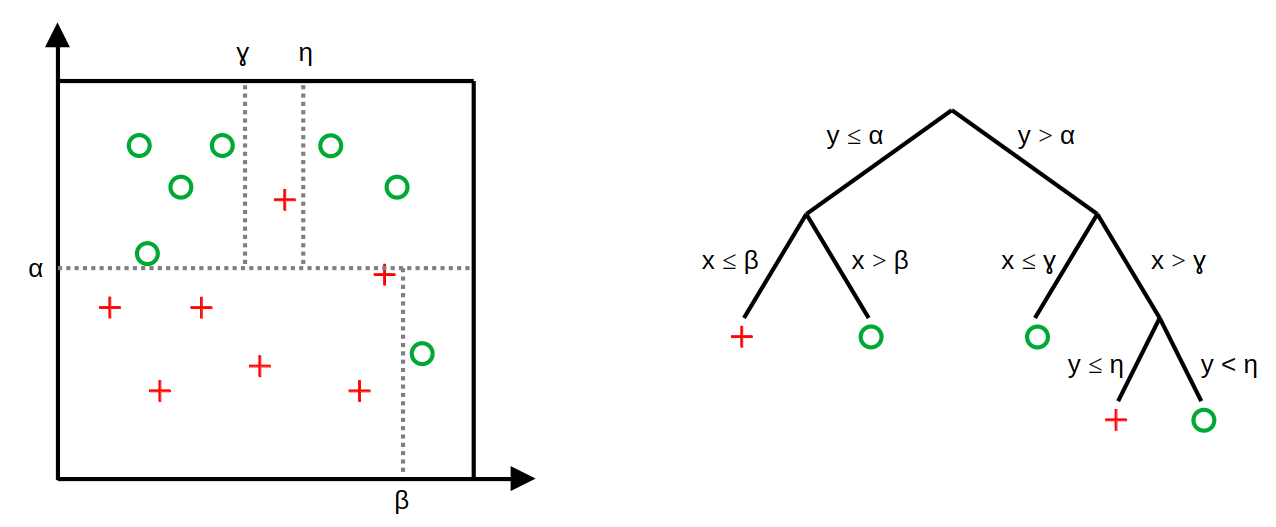
\includegraphics[width=\linewidth]{lecon/15-ml/arb_dec.png}
\end{idee}

\begin{definition}
	Définissons l'entropie d'une partie $S$ de $E$ : $H(S) = \sum\limits_{c \in C} \dfrac{|S\cap c|}{|S|} \times \log\left(\dfrac{|S\cap c|}{|S|}\right)$
\end{definition}

\begin{rem}
	Si tous les éléments ont la même classe, $H(S) = 0$
\end{rem}

\begin{definition}
	Le gain d'une partition $S_1$, $S_2$ de $S$ est : $$H(S) - \left( \dfrac{|S_1|}{|S|} \times H(S_1) + \dfrac{|S_2|}{|S|} \times H(S_2) \right)$$	
\end{definition}

\begin{algo}
	On construit récursivement notre arbre de décision sur notre ensemble S de données restantes:
	\begin{itemize}[label=$\bullet$]
		\item Si $S$ est vide : Choisir la classe la plus représentée du nœud parent
		\item Si toutes les données de $S$ ont la même classe : en faire une feuille avec cette classe.
		\item Sinon, on choisit la coordonnée $i$ et la valeur $m$ tel que la partition $$ S_1 = \left\{ (x_1, \dots, x_n) \in S / x_i \leq m\right\} \text{ et } S_2 = \left\{ (x_1, \dots, x_n) \in S / x_i > m\right\}$$ maximise le gain
	\end{itemize}
\end{algo}

\begin{rem}
	On atteint très vite du sur apprentissage. Pour éviter cela, on peut élaguer le bas de l'arbre (algorithme de Cart)
\end{rem}

\begin{exercise}
	Application à détecter la langue d'une page wikipedia à partir de la matrice de fréquence de facteurs de 2 lettres.
\end{exercise}

\begin{com}
	Ici pour ce TD, on peut mentionner à l'oral le fait qu'on peut utiliser ce truc pour de vrais, et surtout que on peut éventuellement faire réfléchir les élèves à comment modéliser le problème. Fréquence des mots, KNN avec distance de levenstein, fréquence des facteurs de 1, 2, 5 lettres ? Ce qui rend tout ca très intéressants selon moi. (suivant le nombre de pages en exemples, on peut prendre les facteurs d'un certain nombres de lettres (on aura un tableau de taille $27^{\text{taille des facteurs}}$) et ensuite faire du KNN, de l'arbre de décision, etc...) (Avec 4000 pages par langues pour 13 langues, et les facteurs de 2 mots, on classifie très bien).
\end{com}

\begin{rem}
	Dans le cas d'une régression, on peut prendre comme mesure d'impureté la variance.
\end{rem}

\subsection{Représentation de la qualité des classes}

Quand on mesure la performance de notre algorithme on peut chercher à représenter la qualité de nos prédictions (pour classification).

\begin{definition}[matrice de confusion]
	On associe $Y$ à $\{1, \dots, n\}$. La matrice de confusion est alors la matrice carrée $M$ de taille $n$ tel que $M_{i,j}$ est le nombre d'éléments de la classe $i$ qui ont été classés à $j$
\end{definition}

\begin{proposition}
	Plus notre algorithme est correcte, plus la diagonale est dominante.
\end{proposition}

\section{Apprentissage non supervisé}

\begin{rem}
	Il existe plusieurs types d'apprentissage non supervisé. On peut par exemple penser à la réduction de dimension : On a $X\subset \mathbb R^n$ et on cherche $f : X \to \mathbb R^m$ avec $n < m$ et tel que $f(x)$ et $f(y)$ sont proches si $x$ et $y$ le sont aussi.
	
	On se concentrera sur ce qu'on appellera regroupement, (clustering en anglais, ou classification non supervisée) qui consiste à trouver $f : X \to \{1, ..., k\}$ essayant de regrouper les éléments les plus proches.
\end{rem}

\begin{example}
	On a un manuscrit dans un alphabet inconnu, et on cherche à savoir quels lettres sont les mêmes.
\end{example}

\begin{exercise}
	Dans l'exemple au dessus, quel $X$ prendre ?
\end{exercise}

\subsection{Classification hiérarchique ascendante}

\begin{idee}
	Chacun est seul dans sa classe au début, et tant qu'on a $k$ classes, on fusionne les classes les plus proches.
\end{idee}

\begin{rem}
	C'est un algorithme glouton
\end{rem}

\begin{rem}
	Pour définir la distance entre deux classes, on prendre prendre : \begin{itemize}[label=$\bullet$]
		\item $d(S_1, S_2) = \min\limits_{x \in S_1, y \in S_2} (d(x, y))$
		\item $d(S_1, S_2) = \min\limits_{x \in S_1, y \in S_2} (d(x, y))$
		\item $d(S_1, S_2)  = \dfrac{1}{|S_1| \times |S_2|} \sum\limits_{x \in S_1, y \in S_2} d(x, y)$
	\end{itemize}
\end{rem}

\begin{exercise}
	Activité : Représenter l'exécution de l'algorithme sur un dendrogramme
\end{exercise}

\subsection{ALgorithme des $k$-moyennes}

\begin{idee}
	On cherche à trouver $S_1, \dots, S_k$ une partition de $X$ et $z_1, \dots, z_k \in \mathbb R^d$ minimisant $\sum\limits_{i = 1}^{k} \sum\limits_{x \in S_i} d(x, z_i)$
\end{idee}

\begin{algorithm}
	\caption{K-mean}
	Assigner à chaque valeur une classe aléatoire\\
	\Repeter{stabilisation}
	{
		\Pour{$x \in X$}
		{
			assigner à $x$ la classe de $\argmin\limits_{i \in \{1, \dots, k\}} d(x, z_i)$
		}
		\Pour{$i$ allant de $1$ à $k$}
		{
			$z_i \gets \dfrac{1}{|S_i|} \sum\limits_{x \in S_i} x$
		}
	}	
\end{algorithm}

\begin{proposition}
	Cet algorithme termine
\end{proposition}

\begin{proof}
	La cible diminue à chaque étape, et ne peut prendre qu'un nombre fini de valeurs.
\end{proof}

\begin{rem}
	On ne trouve pas toujours le minimum, on tombe souvent dans un minimum local. On relance alors plusieurs fois l'algorithme (d'où l'aléatoire au début).
\end{rem}

\begin{exercise}
	TP sur la réduction de palette d'une image
\end{exercise}

\begin{rem}
	Comment choisir $k$ ? Pour la classification hierarchique ascendante, on s'arrête au plus grand saut sur le dendrogramme, pour les k-moyennes, on affiche la cible finale en fonction de $k$ , et on choisit $k$ au changement de pente.
\end{rem}

\begin{com}
	Bon la faudrait faire les deux dessins mais à très court terme j'ai la flemme.
\end{com}

\chapter{Exemples d'algorithmes pour l'étude des jeux} \label{L16}
\dev{Emile Martinez}{}

La théorie des jeux s'intéresse aux interactions entre des individus (joueurs) qui effectuent des choix selon les règles d'un jeu.

\section{Jeux d'accessibilité à deux joueurs}

\subsection{Définition}

\paragraph{Notation :} Pour $G = (S, A)$, on note $Fin(G) = \{v \in S / deg^+(v) = 0\}$

\begin{definition}
	\label{16-def-jeu}
	Un jeu à deux joueurs est :\begin{itemize}
		\item une arène : un graphe orienté biparti $G = (S_1 \sqcup S_2, A)$
		\item un sommet de départ $s_0$
		\item une partition de $Fin(G) = G_1 \sqcup G_2 \sqcup N$
	\end{itemize}
\end{definition}

\begin{com}
	On peut mentionner ici qu'on peut se restreindre au graphes bipartie, car si quand on joue, c'est à nouveau à nous, on considère les deux coups à jouer d'affilée comme un seul. Mais y a des jeux où on peut rejouer, il faut alors travailler un peu pour modéliser.
\end{com}

\begin{idee}
	Les sommets de $S_1$ sont ceux où J1 joue. Un arc $x \to y$ représente un coup possible pour le joueur qui contrôle l'état $x$, qui déplace alors le jeu dans l'état $y$. $G_i$ sont les états gagnants pour Ji, $N$ ceux d'une partie nulle.
\end{idee}

\begin{example}
	Représentation d'un échantillon de la modélisation du Tic-Tac-Toe\\
	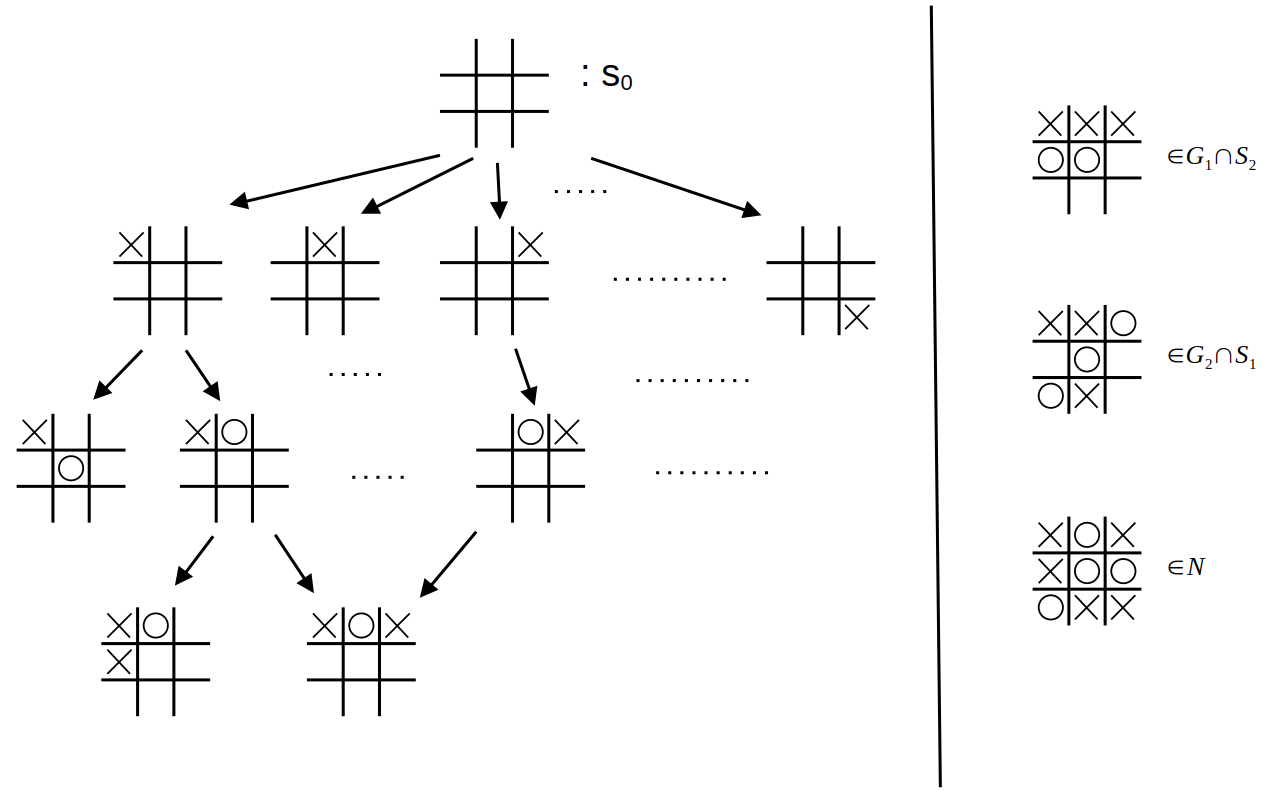
\includegraphics[width=\linewidth]{lecon/16-jeu/tic-tac-toe.png}
\end{example}

\begin{definition}[Partie]
	Une partie d'un jeu $(G, s_0, G_1, G_2, N)$ est un chemin de $s_0$ à un sommet $s_f \in Fin(G)$.
\end{definition}

\begin{definition}
	On appelle stratégie pour le joueur $i \in \{1, 2\}$ toute fonction $\varphi : V_i \to V$ tel que $\forall u \in V_i \backslash Fin(G), \, (u, \varphi(u)) \in A$.
\end{definition}

\begin{com}
	Ici on définit directement une stratégie sans mémoire, le programme se limitant à cela, et les jeux que nous considérerons ne nécessitant pas de stratégie avec mémoire.
\end{com}

\begin{definition}[Stratégie gagnante]
	$\varphi$ est une stratégie gagnante pour le joueur $i$ si pour toute partie $P = s_0, \dots, s_f$,
	$$ \Big( \forall j \in \llbracket O, f-1 \rrbracket, s_j \in V_i \implies s_{j+1} = \varphi(s_j) \Big) \implies s_f \in G_i$$
	$s$ est une position gagnante s'il existe une stratégie gagnante depuis $s$.
\end{definition}

\begin{idee}
	$\varphi$ est une stratégie gagnante si quand les coups de Ji sont ceux de $\varphi$, alors Ji gagne indépendamment de ce que joue l'autre joueur. 
\end{idee}

\subsection{Attracteurs}

On se place du point de vue du joueur 1, mais la situation est symétrique avec le joueur 2.

\begin{definition}[Attracteur]
	Pour une arène $(G, s_0)$, et $F \subset V$ on note $Attr_i(F)$, l'ensemble des sommets depuis lesquels le joueur J1 a une stratégie pour arriver dans $F$ en au plus $i$ étapes. On note $Attr(F) = \bigcup\limits_{i = 0}^{+\infty} Attr_i(F)$
\end{definition}

\begin{proposition}
	Pour un jeu $(G, s_0, G_1, G_2, N)$, $Attr(G_1)$ est l'ensemble des position gagnante de J1.
\end{proposition}

\begin{proposition}\enspace
	\begin{itemize}[label=$\bullet$]
		\item $Attr_0(F) = F$
		\item $Attr_{i+1}(F) = Attr_i(F) \: \cup \: \{u \in V_1 \, / \, \mathcal N^+(u) \cap Attr_i(F) \neq \emptyset\} \: \cup \: \{u \in V_2 \, / \, \mathcal N^+(u) \subset Attr_i(F)\} $
	\end{itemize}
\end{proposition}

\begin{proposition}
	Si $G$ est fini alors $\left( Attr_i(F) \right)$ est croissante bornée, donc stationnaire. Sa limite est alors $Attr(F)$.
	
	Une stratégie gagnante depuis $Attr(F)$ est :
	$$ \begin{array}{rcl}
		\varphi : V_1 & \to V\\
		v & \mapsto & \left\{ \begin{array}{ll}
			\omega \in \mathcal N^+(v) \cap Attr_i(F) & \text{si } v \in Attr_{i+1}(F) \backslash Attr_i(F)\\
			\omega \in \mathcal N^+(v) & \text{si } v \notin Attr(F)
		\end{array} \right.
	\end{array} $$
\end{proposition}

\paragraph{Développement :} Stratégies gagnantes pour le jeu de Nim à 1 puis plusieurs tas.

\section{Jeux Min-Max}

\subsection{Algorithme Min-Max}

On considère ici des jeux à deux joueurs, en reprenant la définition \ref{16-def-jeu} en  remplaçant la partition de $Fin(G)$ par une fonction de coût $c : Fin(G) \to \mathbb Z$.

Le joueur 1 (appelé Max ici) essaye alors de maximiser par ses coups la valeur finale, et le joueur 2 (ici Min) essaye de la minimiser.

\begin{rem}
	La partie précédente en est un cas particulier avec $c(G_1) = 1$, $c(N) = 0$ et $C(G_2) = 1$ 
\end{rem}

\begin{definition}
	Une stratégie optimale pour le joueur Max (resp. Min) est une stratégie maximisant (resp. minimisant) le coût.
\end{definition}

\begin{algo}
	On fait une recherche exhaustive de tous les coups, en prenant à chaque fois celui ayant le résultat maximum (resp.minimimum) quand Max (resp. Min) joue. Cela détermine une stratégie optimale (pour les deux joueurs).
\end{algo}

\begin{rem}
	En pratique, c'est souvent infaisable tant le graphe est gros.
	\begin{example}
		Les echecs, avec +1000 victoire blanche, -1000 victoire noire et 0 nulle, le graphe a plus de $10^44$ sommets.
	\end{example}
\end{rem}

\begin{definition}
	Une heuristique $h : V \to \mathbb Z$ est une estimation de à quoi mènerait dans le meilleur cas cette position
\end{definition}

\begin{com}
	Ici on a une définition formelle avec l'intuition de son interprétation (et donc de son usage). (une heuristique, c'est simplement une fonction $V \to \mathbb Z$)
\end{com}

\begin{example}
	La fonction qui aux échecs donne la somme de la valeur des pièces
\end{example}

\begin{idee}
	On fait l'exploration exhaustive en renvoyant l'heuristique quand on a fait suffisament d'étapes.
\end{idee}

\begin{algorithm}[H]
	\caption{$MinMax(j, prof, u)$}
	\Si{$u \in Fin(G)$ ou $prof = 0$}
		{\Retour{$h(u)$}}
	\eSi{$i == 1$}
		{$f\gets \max$}
		{$f \gets\min$}
	\Retour{$f\Big(\Big\{MinMax(3-j, \,prof-1, \,v) \enspace \big/ \enspace v \in \mathcal N^+(u)\Big\}\Big)$}
\end{algorithm}

\subsection{Élagage $\alpha$-$\beta$}

\begin{minipage}{0.5\linewidth}
	\begin{idee}
		Il n'est pas nécessaire d'explorer tout l'arbre : si je suis Min et que Max au coup d'avant peut faire 5 avec un autre coup, dès que je vois que je peux faire 1, je peux arrêter d'explorer, car je sais que Max ne fera pas ce coup.
	\end{idee}
\end{minipage} \quad \begin{minipage}{0.4\linewidth}
	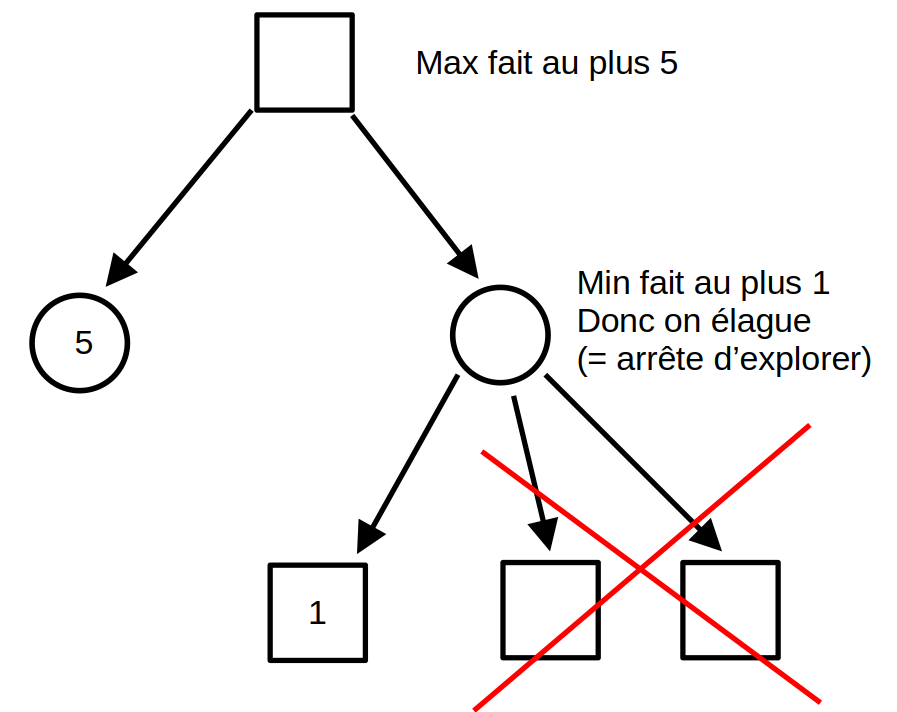
\includegraphics[width=\linewidth]{lecon/16-jeu/alpha_beta.png}
\end{minipage}

\begin{algorithm}[H]
	\caption{$Alphabeta(j, \alpha, \beta, u)$}
	\Si{$u \in Fin(G)$}
		{\Retour{$c(u)$}}
	\eSi{$joueur = 1$}
	{
		$res \gets -\infty$\\
		\Pour{$v$ voisin de $u$}
		{
			$e = Alphabeta(2, \max(res, \alpha), \beta, v)$\\
			\eSi{$e > \beta$}
				{\Retour{$e$}\quad \tcp{Élagage}}
				{$res \gets \max(e, res)$}
		}
		\Retour{$res$}
	}
	{
		\tcp{Symétrique, à faire en exercice}
	}
\end{algorithm}

\begin{idee}
	$\alpha$ (resp. $\beta$) est la valeur maximale (resp. minimale) que peut faire Max (resp. Min) parmi ce que l'on a explorer pour l'instant. (On appelle donc $alphabeta(1, -\infty, +\infty, s_0)$)
\end{idee}

\begin{rem}
	Cet algorithme est exact. On peut, comme pour Min-Max ajouter une profondeur et une heuristique.
\end{rem}

\begin{exercise}
	Comparaison des temps d'exécution de Min-Max et de Alpha-Beta pour le Tic-Tac-Toe (exploration complète sans heuristique).
\end{exercise}

\section{Les Jeux à un joueur}

\subsection{Graphe d'état}

\begin{definition}
	Un graphe d'état est la donnée d'un graphe orienté $G = (S, A)$ pondéré par $c : A \to \N$, d'un état initial $s_0$ et d'un ensemble d'états finaux $F \subset S$
\end{definition}

\begin{rem}
	$S$ représente les configurations d'un jeu à un joueur, $A$ les transitions d'une configuration à une autre en un coup, $c$ le coût de cette transition, et $F$ les configurations gagnantes. 
\end{rem}

\paragraph{Objectif :} Trouver un chemin dans ce graphe entre l'état initial et l'un des états finaux de coût total minimal.

\begin{example}
	Dans le jeu du taquin, les états correspondent aux dispositions possibles du plateau. L'état final est le plateau remis dans l'ordre. Chaque case a un degré sortant inférieur ou égal à 4 qui correspond aux déplacements possibles de la case vide (vers le haut, le bas, à gauche ou à droite). Tous les déplacements ont un coût unitaire.
\end{example}

\begin{rem}
	le graphe d'état est en général trop gros pour être stocké entièrement en mémoire. Il est donc nécessaire de mettre en place des stratégies ou des heuristiques pour orienter la recherche du chemin
\end{rem}

\subsection{L'algorithme A*}

\begin{principe}
	L'algorithme A* est une variante de l'algorithme de Dijkstra pour calculer un plus court chemin entre un sommet initial $s_0$ et un sommet final $s_f$. On visite les sommets par estimation de leur proximité à $s_f$ grâce à une fonction $f$ définie par:
	
	$f(s) = d(s) + h(s)$ où $d(s)$ est le coût d'un plus court chemin entre $s_0$ et $s$ et $h(s)$ i une estimation (heuristique) du coût entre $s$ et $s_f$
\end{principe}

\begin{example}
	dans le cas du taquin, on peut penser aux heuristiques suivantes :
	\begin{itemize}[label=$\bullet$]
		\item nombre de chiffres mal placés 
		\item somme des distances de Manhattan des cases à leur position finale
	\end{itemize}
\end{example}

\begin{algorithm}[H]
	\Entree{W la matrice de poids du graphe;
		h le tableau pour l'heuristique;
		$s_{0}$ et $s_{f}$ les sommets initiaux et finaux}
	\Sortie{la distance d'un plus court chemin de $s_{0}$ à $s_{f}$}
	
	$D \gets$ tableau initialisé à $\infty$\\
	$D[s_{0}] \gets$ 0\\
	$P \gets$ file de priorité vide\\
	Ajouter $(s_{0}, h[s_{0}])$ à $P$\\
	\Tq{$P$ non vide}{
		$(s, \_) \gets$ $extraire(P)$\\
		\Si{$s = s_{f}$}{\Retour{$D[s]$}}
		\Pour{$s'$ successeur de $s$}{
			$c \gets D[s] + W[s, s']$\\
			\Si{$c < D[s']$}{
				$D[s'] \gets c$\\
				Ajouter  $(s', c+h[s'])$ à $P$\\
			}
		}
	}
	\Retour{NonAccessible}
	\caption{Algorithme A*}
\end{algorithm}

\begin{rem}
	Si $h = 0$, on retrouve Dijkstra
\end{rem}

\begin{definition}
	Une heuristique est dite admissible si $\forall u \in S, h(u) \leq d(u)$
\end{definition}

\begin{theorem}[Correction]
	Si $h$ est admissible, alors A* renvoie la distance d'un court chemin de $s_0$ à $s_f$.
\end{theorem}

\begin{definition}
	Une heuristique est dite monotone si $\forall (u,v) \in A, h(u) \leq h(v) + w(u,v)$
\end{definition}

\begin{rem}
	Dans un graphe avec les distances euclidiennes entre nœuds, la distance à vol d'oiseau est une heuristique monotone.
\end{rem}

\begin{proposition}
	Si $h$ est monotone et $h(s_f) = 0$, alors A* est correct ($h$ est admissible) et extrait chaque noeud au plus une fois.
\end{proposition}

\paragraph{Développement :} Démonstration du théorème et de la propriété précédente.

\begin{appl}
	Calcul des itinéraires par un GPS
\end{appl}

\chapter{Algorithmes d'ordonnancement de tâches et de gestion de ressources} \label{L17}
\dev{Emile Martinez}{}

\paragraph{Métaphore filée :} Ordonnancement des tâches dans une cuisine.

\section{Motivation : le système d'exploitation}

\begin{rem}
	Lorsque vous utilisez votre PC, vous éxécutez des dizaines de programmes "en même temps" (lecture de mail, taper au clavier, écouter de la musique...). Pourtant, votre PC a un nombre limité de processeurs.
\end{rem}

\begin{definition}[Execution concurrente et ordonnanceur]
	Le système d'exploitation peut interrompre un processus en cours pour exécuter du code qui lui est propre. Il peut alors, à intervalles réguliers, décider à quelle tâche en cours il rend la main. 
	
	Le rôle de l'ordonnanceur est de choisir le prochain processus à exécuter parmi une liste de processus candidats. 
\end{definition}

%\begin{tikzpicture}[->, node distance=2cm]
%	
%	\node (q0) {};
%	\node[state, right=of q0] (pret) {Prêt};
%	\node[state, right=of pret] (elu) {Élu};
%	\node[state, below right=of pret] (blo) {Bloqué};
%	\node[state, right of= elu] (term) {Terminé};
%	
%	\draw (q0) edge[] (pret);
%	\draw (pret) edge[bend left] (elu);
%	\draw (elu) edge[bend left] (pret);
%	\draw (elu) edge[bend left] (blo);
%	\draw (blo) edge[bend left] (pret);
%	\draw (elu) edge[] (term);
%	
%	
%\end{tikzpicture}

\begin{center}
	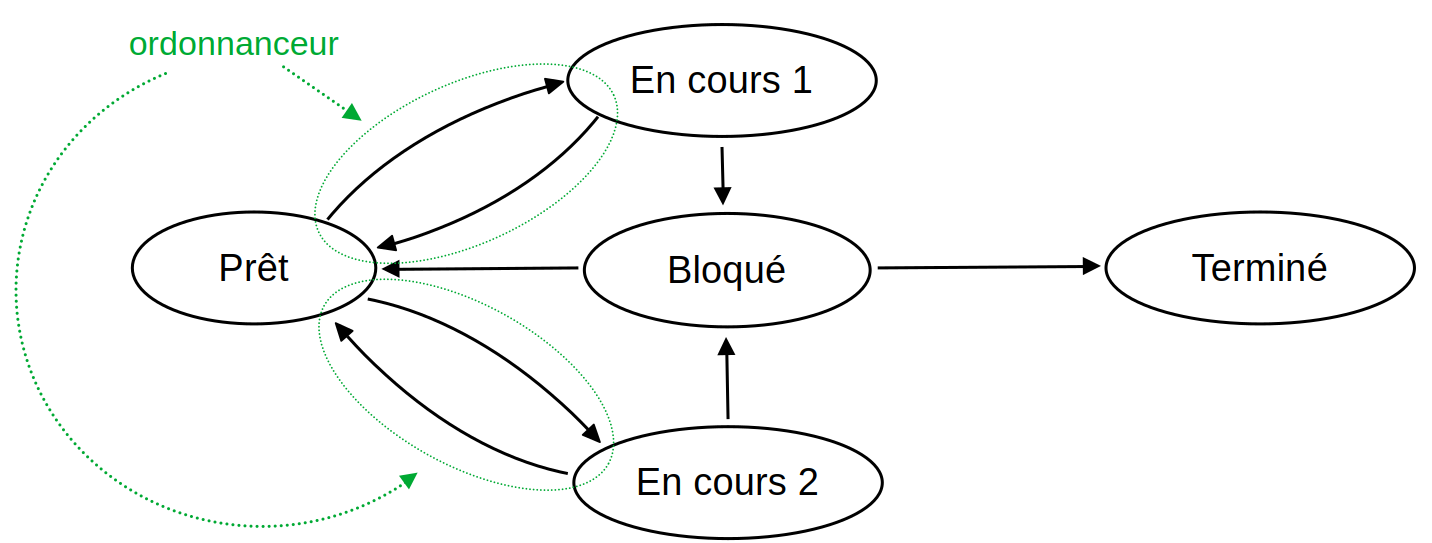
\includegraphics[width=0.9\linewidth]{lecon/17-ordonnancement/graphe_etat.png}\\
	Cycle de vie d'un processus
\end{center}

\begin{com}
	A faire. Mais à comparer avec le truc de Malory, parfois mieux que notre truc à nous.
\end{com}

\chapter{Gestion et coordination de multiples fils d'exécution} \label{L18}
\dev{Emile Martinez}{}

\section{Gestion par la machine (Terminale)}

\subsection{Motivation}

Lorsque vous utilisez votre PC, vous éxécutez des dizaines de programmes «en même temps» (lecture de courriel, taper au clavier, écouter de la musique...). Pourtant, votre PC a un nombre limité de processeurs. Comment fonctionne cette illusion ?

\subsection{Exécution concurrente}

\begin{definition}
	Un processus est un programme en cours d'exécution sur un ordinateur. Il dispose d'une zone mémoire en RAM. Le système d'exécution identifie les processus grâce à un numéro unique appelé PID.
\end{definition}

\begin{definition}[Exécution concurrente]
	Deux processus s'exécutent en concurrence si les intervalles entre leur commencement et leur fin respective sont non disjoints.
\end{definition}

\begin{principe}[Fonctionnement de l'exécution concurrente]
	Le système d'exploitation peut interrompre un processus en cours pour exécuter du code qui lui est propre. Il peut alors, à intervalles réguliers, décider à quelle tâche en cours il rend la main. 
	
	Le rôle de l'ordonnanceur est de choisir le prochain processus à exécuter parmi une liste de processus candidats. 
\end{principe}

\begin{center}
	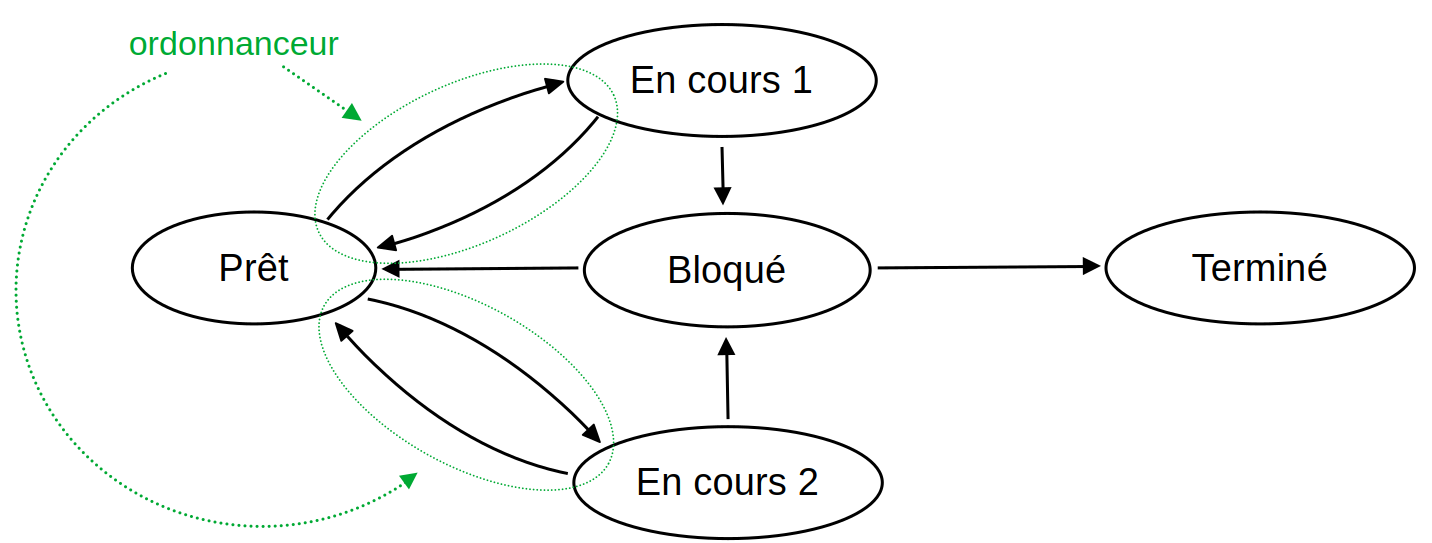
\includegraphics[width=0.9\linewidth]{lecon/17-ordonnancement/graphe_etat.png}\\
	Cycle de vie d'un processus
\end{center}

\subsection{L'ordonnanceur}

On peut vouloir des garanties sur la manière dont l'ordonnanceur choisit ses tâches.

\begin{definition}
	On dit qu'il y a absence de famines (ou vivacité) si aucun processus n'attend indéfiniment.
\end{definition}

\begin{definition}
	On dit qu'il y a équité si aucun processus n'est favorisé.
\end{definition}

\begin{algo}[Algorithme du tourniquet]
	L'ordonnanceur définit un intervalle de temps $\tau$. 
	
	Il place les processus en attente dans une file selon leur ordre d'arrivée (PAPS).
	
	Tant que la file est non vide, il en sort le premier et l’exécute durant tau. Si besoin, il le ré-insert en queue de file.
\end{algo}

\begin{example} Exemple d'exécution sur 3 processus et un seul processeur\\
	\begin{center}
		
		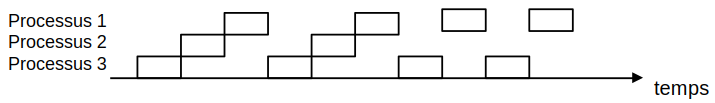
\includegraphics[width=0.8\linewidth]{lecon/18-fil/tourniquet.png}
	\end{center}
\end{example}

\begin{proposition}
	L'algorithme du tourniquet garantie l'équité et l'absence de famine.
\end{proposition}

\begin{rem}
	Certains processus étant plus importants que d'autres, on peut adapter le temps tau à chaque processus, en fonction de leur priorité.
\end{rem}

\subsection{Commande unix de gestion de processus}

\noindent \begin{minipage}{0.3\linewidth}
	\begin{lstlisting}
$ ps
	\end{lstlisting}
\end{minipage}\quad\begin{minipage}{0.6\linewidth}
	permet d'afficher les processus en cours, et leur taux d'occupation du processeur et de la mémoire. 
\end{minipage}\\

\noindent \begin{minipage}{0.3\linewidth}
	\begin{lstlisting}
$kill 6555
	\end{lstlisting}
\end{minipage}\quad\begin{minipage}{0.6\linewidth}
	envoie un  signal de terminaison au processus de PID 6555. (Pour une application graphique, c'est ce que fait la croix rouge)
\end{minipage}\\

\noindent \begin{minipage}{0.3\linewidth}
	\begin{lstlisting}
$top
	\end{lstlisting}
\end{minipage}\quad\begin{minipage}{0.6\linewidth}
	affiche la liste des processus prêts et en cours.
\end{minipage}

\section{Gestion par l'utilisateur (prépa)}

\subsection{Motivation}

\begin{definition}
	Un fil d'exécution (thread en anglais) est un sous processus qui partage la mémoire avec les autres fils du processus.
\end{definition}

\begin{impl}
	En C, un programme peut lancer d'autres fils d'exécution, de type \texttt{pthread\_t} et que l'on lance avec la fonction \texttt{pthread\_create}
\end{impl}

\begin{idee}
	On peut alors gérer des choses en parallèle
\end{idee}

\begin{example}
	\label{18-somme-para} \normalfont
	Somme parallélisée d'un tableau T de taille 2m.\\\\
	\begin{minipage}{0.45\linewidth}
		Fil 1 :
		\begin{lstlisting}[style=CStyle]
for(int i = 0; i < m; i++){
	int s = res + T[2*i];
	res = s;  }\end{lstlisting}
	\end{minipage} \quad
	\begin{minipage}{0.45\linewidth}
		Fil 2:
	\begin{lstlisting}[style=CStyle]
for(int i = 0; i < m; i++){
	int s = res + T[2*i + 1];
	res = s;  }\end{lstlisting}
	\end{minipage}\\
	On peut donc aller deux fois plus vite.
	
	\paragraph{Question :} Que se passe-t-il sur l'exécution F1:1 $\to$ F2:2 $\to$ F1:3 $\to$ F2:3 ?
\end{example}

\subsection{Les verrous}

\begin{definition}
	Le problème de l'exclusion mutuelle consiste à garantir que deux fils d'exécution n'essaieront pas d'exécuter simultanément un morceau de code prédéfini.
\end{definition}

\begin{example}
	Les lignes 2 et 3 pour les fils 1 et 2 de l'exemple \ref{18-somme-para}.
\end{example}

\begin{definition}
	Un verrou (ou mutex) est une structure de données permettant deux opérations : \begin{itemize}
		\item \texttt{prendre()} : appel bloquant qui demande l'accès au verrou
		\item \texttt{rendre()} : appel qui libère le verrou
	\end{itemize}
\end{definition}

\begin{proposition}
	Une implémentation efficace des verrous devrait garantir l'exclusion mutuelle, l'absence de famine et l'équité.
\end{proposition}

\begin{algo}
	L'algorithme de Peterson propose une implémentation des verrous pour deux fils vérifiant ces propriétés.
\end{algo}

\paragraph{Développement :} Présentation de l'algorithme de Peterson et preuve de fonctionnement.

Extension à n fils d'exécution :
\begin{algo} \normalfont Algorithme de la boulangerie de Lamport\\
\begin{minipage}{0.6\linewidth}
	\begin{lstlisting}[style=CStyle]   
void prendre(int i ){
	Acq[i] = 1;
	int t = 0;
	for(int j = 0; j < n; j++)
		t = MAX(t, num[j]);
	num[i] = t + 1;
	Acq[i] = 0;
	
	for(int j = 0; j < n; j++){
		while (acq[j] == 1);
		while (num[j] == 1 && (num[j] < num[i] 
			|| (num[j] == num[i] && j < i)) );
	}
}

void rendre(int i){
	num[i] = 0;
}\end{lstlisting}
\end{minipage}
\begin{minipage}{0.25\linewidth}
	$\begin{array}{l}
	\left. \begin{array}{c} \\ \\ \\ \\ \\ \end{array} \right\} \begin{array}{c} \\ \\ \text{Obtenir un} \\\text{numéro} \\ \\ \end{array} \\
	\\
	\left. \begin{array}{c} \\ \\ \\ \\ \end{array} \right\} \begin{array}{c} \\ \text{Attendre son} \\\text{tour pour prendre} \\ \text{le verrou} \\ \end{array}
	\\ \\ \\ \\ \\
	\end{array}
	$
\end{minipage}
\end{algo}

\paragraph{Analogie :} On prend un ticket dans une boulangerie, et on attend que ce soit notre tour.

\begin{rem}
	L'attente ici est active (on effectue des opérations quand on attend)
\end{rem}

\begin{impl}
	\normalfont
	En C : Les verrous sont disponibles dans la bibliothèque pthread. \begin{itemize}[label=]
		\item type : \texttt{pthread\_mutex\_t}
		\item initialisation : \texttt{pthread\_mutex\_init(pthread\_mutex\_t *m, NULL)}
		\item prendre : \texttt{pthread\_mutex\_lock(pthread\_mutex\_t *m)}
		\item rendre : \texttt{pthread\_mutex\_unlock(pthread\_mutex\_t *m)}
	\end{itemize}
\end{impl}

\begin{rem}
	Une mauvaise utilisation des verrous peut créer des interblocages.
\end{rem}

\begin{example} \enspace\\ \normalfont
	\begin{minipage}{0.3\linewidth}
	Fil 1 :
	\begin{lstlisting}[style=CStyle]
prendre(m1);
prendre(m2);\end{lstlisting}
\end{minipage} \quad
\begin{minipage}{0.3\linewidth}
	Fil 2:
	\begin{lstlisting}[style=CStyle]
prendre(m2);
prendre(m1);\end{lstlisting}
\end{minipage}
\end{example}

\begin{com}
	Ici on ne prend pas un exemple plus gros, comme le dîner des philosophes, car ici on ne veut pas s'étendre sur ça, simplement faire une ouverture, et mentionner le problème.
\end{com}

\section{Les sémaphores}

\paragraph{Analogie :} Tableau des clés d'un hôtel

\begin{definition}
	Un sémaphore est un compteur qui propose les opérations suivantes :
	\begin{itemize}
		\item Initialiser à une valeur entière
		\item décrémenter : appel bloquant, décrémente le compteur s'il est positif, attend qu'il le soit sinon
		\item incrémenter : incrémente le compteur. S'il devient positif, cela libère un fil si un attendait
	\end{itemize} 
\end{definition}

\begin{appl}
	Limiter l'accès à une ressource à $n$ fils.
\end{appl}

\begin{com}
	On ne s’appesantit pas sur cette application au vu de sa complexité. Donc même si c'est l'application la plus directe et que dans un vrai cours, on aurait peut-être ici un petit programme l'utilisant pour illustrer le concept, on se concentre nous sur des choses plus importantes.
\end{com}

\begin{rem}
	On peut implémenter un verrou par un sémaphore initialisé à 1.
\end{rem}

\begin{impl}
	Les sémaphores sont disponibles dans la bibliothèque semaphore.h.
	\begin{itemize}
		\item type : \texttt{sem\_t}
		\item initialisation : \texttt{sem\_init}
		\item décrémenter : \texttt{sem\_wait}
		\item incrémenter : \texttt{sem\_post}
	\end{itemize}
\end{impl}

\begin{proposition}
	L'implémentation des sémaphore est faites (normalement) sans attente active.
\end{proposition}

\begin{appl}[Problème du rendez-vous]
	On a p fils qui doivent se synchroniser. Chacun travaillant en deux phases. Dans la première phase, tous les fils sont indépendants et peuvent s’exécuter simultanément. La deuxième phase d'un fil ne peut débuter que si tous les fils ont terminé la première.\\
	
	On peut résoudre ce problème à l'aide de sémaphore.
\end{appl}

\paragraph{Développement :} Solutions aux problèmes du rendez-vous

\begin{appl}[Producteur / Consommateur] \normalfont
	On dispose d'un tampon de taille N, et on a deux types de fils : \begin{itemize}
		\item des producteurs qui produisent des ressources et les stockent dans le tampon
		\item des consommateurs qui consomment les données produites (consommer une donnée libère son emplacement)
	\end{itemize}
	
	Pour que la donnée consommée soit la plus vieille, le tampon est circulaire :
	\begin{center}
		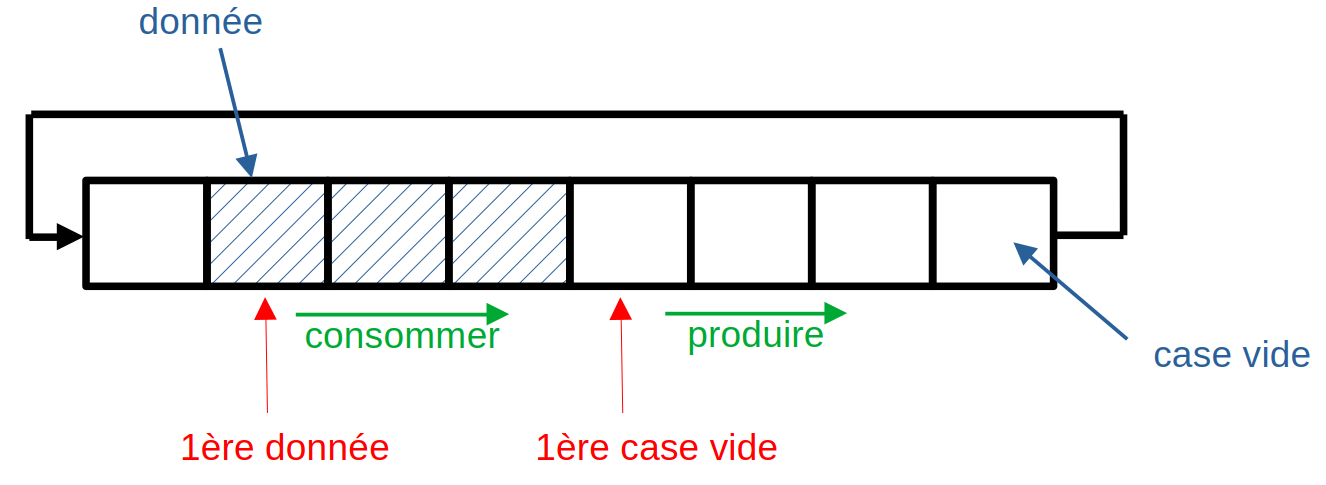
\includegraphics[width=0.7\linewidth]{lecon/18-fil/prod-cons.png}
	\end{center}
	
	\paragraph{Problème :} \begin{itemize}
		\item l'accès au tampon est partagé
		\item les consommateurs doivent attendre qu'une place soir produite
		\item les producteurs doivent attendre que de la place soit libérée dans le tampon.
	\end{itemize}
	
	\paragraph{Solution :} On utilise un sémaphore indiquant le nombre données disponibles et un le nombre de cases disponibles.
	
	\begin{lstlisting}[style=CStyle]
sem_t mutex, vide, plein;
sem_init(&mutex, 0, 1);
sem_init(&vide, 0, N);
sem_init(&plein, 0, 0);\end{lstlisting}

\begin{minipage}{0.45\textwidth}
		Producteur :
		\begin{lstlisting}[style=Cstyle]
int item;
while(1){
	item = produire_item()
	// On attend un place
	sem_wait(&vide);
	sem_wait(&mutex);
	insert_item(item);
	sem_post(&mutex);
	// On la remplie
	sem_post(&plein);
}\end{lstlisting}
	\end{minipage}\qquad
	\begin{minipage}{0.45\textwidth}
		Consommateur :
		\begin{lstlisting}[style=Cstyle]
int item;
while(1){
	// On attend un element
	sem_wait(&plein);
	sem_wait(&mutex);
	item = remove_item();
	sem_post(&mutex);
	// On libere une place
	sem_post(&vide);
	consomer_item(item);
}\end{lstlisting}
	\end{minipage}
	
\end{appl}

\begin{com}
	Par manque de place, on peut moins s'étendre et ne pas écrire l'algorithme, se contenter de dire qu'on a un sémaphore qui compte les places vides et un les places pleines. (et éventuellement virer le dessin)
\end{com}

\begin{rem}
	On peut implémenter un sémaphore par de l'attente active et des verrous. Donc naturellement, ce qu'apporte souvent les sémaphores, par rapport au verrou, c'est moins d'attente active.
\end{rem}

\begin{com}
	Cette remarque, car si on a des élèves un peu rapide, il pourrait trouver assez facilement des solutions n'utilisant que des verrous, et donc se poserait la question de la pertinence des sémaphores dans ce contexte. L'intérêt des sémaphores vient alors de la suppression de l'attente active.
\end{com}

\begin{com}
	On ne mentionne pas tous les problèmes possibles liés aux sémpahores, car ici dans cette leçon on doit parler de plein d'aspects différents. On se limite alors à en expliquer le fonctionnement global et à les illustrer.
\end{com}

\chapter{Mémoire : du bit à l’abstraction vue par les processus.} \label{L19}

\chapter{Problèmes et stratégies de cohérence et de synchronisation.} \label{L20}
\dev{Emile Martinez}{}

\section{Introduction}

\begin{definition}
	Un processus est un programme en cours d'exécution sur un ordinateur. Il dispose d'une zone mémoire en RAM (pour stocker la pile, les données de travail, etc.). Le système d'exécution identifie les processus grâce à un numéro unique appelé PID. 
\end{definition}

\begin{definition}
	Un fil d'exécution (ou thread) est un sous processus qui partage la mémoire avec les autres threads du processus.
\end{definition}

\begin{impl}
	En C, un programme peut lancer d'autres fils d'exécution, de type \texttt{pthread\_t} et que l'on lance avec la fonction \texttt{pthread\_create}
\end{impl}

\begin{example}
	\label{20-somme-para} \normalfont
	Somme parallélisée d'un tableau T de taille 2m.\\\\
	\begin{minipage}{0.45\linewidth}
		Fil 1 :
		\begin{lstlisting}[style=CStyle]
			for(int i = 0; i < m; i++){
				int s = res + T[2*i];
				res = s;  }\end{lstlisting}
	\end{minipage} \quad
	\begin{minipage}{0.45\linewidth}
		Fil 2:
		\begin{lstlisting}[style=CStyle]
			for(int i = 0; i < m; i++){
				int s = res + T[2*i + 1];
				res = s;  }\end{lstlisting}
	\end{minipage}\\
	On peut donc aller deux fois plus vite.
	
	\paragraph{Question :} Que se passe-t-il sur l'exécution F1:1 $\to$ F2:2 $\to$ F1:3 $\to$ F2:3 ?
\end{example}

\subsection{Définitions générales}

\begin{definition}
	On appelle appel bloquant un appel à une fonction qui attendra que les conditions soit réunies avant de terminer.
\end{definition}

\begin{example}
	L'appel à \texttt{recv} en C qui attend que quelque chose arrive pour terminer.
\end{example}

\begin{definition}
	On dit qu'il y a absence de famine (ou vivacité) si aucun fil n'attend indéfiniment.
\end{definition}

\begin{definition}
	On dit qu'il y a équité si aucun processus n'est favorisé.
\end{definition}

\section{Exclusion mutuelle et verrous}

\subsection{Définition}

\begin{definition}
	Une section critique est un ensemble de morceau de code qui ne doit être exécute que par un seul fil à la fois.
	
	Le problème de l'exclusion mutuelle est le problème consistant à garantir qu'on aura toujours au plus un fil dans une section critique.
\end{definition}

\begin{example}
	Les lignes 2 et 3 pour les fils 1 et 2 de l'exemple \ref{20-somme-para}.
\end{example}

\begin{rem}
	Dans une section critique, les morceaux de code ne sont pas forcément les mêmes pour chaque fil (si un fil ne fais que lire quand l'autre ne fais qu'écrire dans une case partagée, leurs codes incompatibles n'est pas le même).
\end{rem}

\paragraph{Solution :} Les verrous

\begin{definition}
	Un verrou (ou mutex) est une structure de données permettant deux opérations : \begin{itemize}
		\item \texttt{prendre()} : appel bloquant qui demande l'accès au verrou
		\item \texttt{rendre()} : appel qui libère le verrou
	\end{itemize}
\end{definition}

\begin{proposition}
	Une implémentation efficace des verrous devrait garantir l'exclusion mutuelle, l'absence de famine et l'équité.
\end{proposition}

\subsection{Implémentation des verrous pour 2 fils}

\begin{definition}
	Une opération est dite atomique si elle ne peut pas être interrompue. Dans notre cas, une opération atomique correspond à une instruction en langage machine. On a notamment les opérations : \begin{itemize}
		\item lire une case mémoire
		\item écrire une case mémoire
		\item effectuer une opération arithmétique/logique
	\end{itemize}
\end{definition}

\begin{rem}
	Attention ! Une opération dans un langage de programmation n'est pas atomique en général.
\end{rem}

\begin{proposition}
	Si deux fils écrivent la même case mémoire simultanément, la case mémoire contiendra soit la valeur du premier fils soit celle du second. De même, si un fil lis dans une case quand un autre écrit, la valeur sera écrite et le premier fil lira la valeur précédente ou la valeur actualisée.
\end{proposition}

\begin{algo}
	Algorithme de Peterson pour un verrou à deux fils \normalfont
	\begin{lstlisting}
tour = -1
veut_entrer = [false, false]

rendre(i): 
	veut_entrer[i] = true
	tour = 1-i

	while(tour == 1-i && veut_entrer[1-i]) {}

prendre(i): 
	veut_entrer[i] = false
	\end{lstlisting}
\end{algo}

\paragraph{Développement :} Présentation de l'algorithme de Peterson.

\subsection{Généralisation à n fils}

\begin{algo} \normalfont Algorithme de la boulangerie de Lamport\\
	\begin{minipage}{0.6\linewidth}
		\begin{lstlisting}[style=CStyle]   
void prendre(int i ){
	Acq[i] = 1;
	int t = 0;
	for(int j = 0; j < n; j++)
	t = MAX(t, num[j]);
	num[i] = t + 1;
	Acq[i] = 0;
	
	for(int j = 0; j < n; j++){
		while (acq[j] == 1);
		while (num[j] == 1 && (num[j] < num[i] 
		|| (num[j] == num[i] && j < i)) );
	}
}

void rendre(int i){
	num[i] = 0;
}\end{lstlisting}
	\end{minipage}
	\begin{minipage}{0.25\linewidth}
		$\begin{array}{l}
			\left. \begin{array}{c} \\ \\ \\ \\ \\ \end{array} \right\} \begin{array}{c} \\ \\ \text{Obtenir un} \\\text{numéro} \\ \\ \end{array} \\
			\\
			\left. \begin{array}{c} \\ \\ \\ \\ \end{array} \right\} \begin{array}{c} \\ \text{Attendre son} \\\text{tour pour prendre} \\ \text{le verrou} \\ \end{array}
			\\ \\ \\ \\ \\
		\end{array}
		$
	\end{minipage}
\end{algo}

\paragraph{Analogie :} On prend un ticket dans une boulangerie, et on attend que ce soit notre tour.

\begin{rem}
	Dans nos implémentations, l'attente est active.
\end{rem}

\begin{impl}
	\normalfont
	En C : Les verrous sont disponibles dans la bibliothèque pthread. \begin{itemize}[label=]
		\item type : \texttt{pthread\_mutex\_t}
		\item initialisation : \texttt{pthread\_mutex\_init(pthread\_mutex\_t *m, NULL)}
		\item prendre : \texttt{pthread\_mutex\_lock(pthread\_mutex\_t *m)}
		\item rendre : \texttt{pthread\_mutex\_unlock(pthread\_mutex\_t *m)}
	\end{itemize}
\end{impl}

\section{Synchronisation et sémaphores}

\begin{impl}
	Pour synchroniser des fils, la commande \texttt{pthread\_join} de la bibliothèque pthread permet à un fil d'attendre la fin et de récupérer la valeur de retour d'un ou de n'importe lequel de ces fil fils.
\end{impl}

\begin{rem}
    Néanmoins, on peut souhaiter plus de synchronisation entre les fils.
\end{rem}

\subsection{Sémaphore et synchronisation}
\textit{Bon on a un peu de redondances sur les titres là}

\paragraph{Analogie :} Tableau des clés d'un hôtel

\begin{definition}
	Un sémaphore est un compteur qui propose les opérations suivantes :
	\begin{itemize}
		\item Initialiser à une valeur entière
		\item décrémenter : appel bloquant, décrémente le compteur s'il est positif, attend qu'il le soit sinon
		\item incrémenter : incrémente le compteur. S'il devient positif, cela libère un fil si un attendait
	\end{itemize} 
\end{definition}

\begin{appl}
	Limiter l'accès à une ressource à $n$ fils.
\end{appl}

\begin{com}
	On ne s’appesantit pas sur cette application au vu de sa complexité. Donc même si c'est l'application la plus directe et que dans un vrai cours, on aurait peut-être ici un petit programme l'utilisant pour illustrer le concept, on se concentre nous sur des choses plus importantes.
\end{com}

\begin{rem}
	On peut implémenter un verrou par un sémaphore initialisé à 1.
\end{rem}

\begin{impl}
	Les sémaphores sont disponibles dans la bibliothèque semaphore.h.
	\begin{itemize}
		\item type : \texttt{sem\_t}
		\item initialisation : \texttt{sem\_init}
		\item décrémenter : \texttt{sem\_wait}
		\item incrémenter : \texttt{sem\_post}
	\end{itemize}
\end{impl}

\begin{proposition}
	L'implémentation des sémaphore est faites (normalement) sans attente active.
\end{proposition}

\begin{appl}[Problème du rendez-vous]
	On a p fils qui doivent se synchroniser. Chacun travaillant en deux phases. Dans la première phase, tous les fils sont indépendants et peuvent s’exécuter simultanément. La deuxième phase d'un fil ne peut débuter que si tous les fils ont terminé la première.\\
	
	On peut résoudre ce problème à l'aide de sémaphore.
\end{appl}

\paragraph{Développement :} Solutions aux problèmes du rendez-vous

\subsection{Cas classique d'utilisation}

\begin{appl}[Problème du rendez-vous]
	On a p fils qui doivent se synchroniser. Chacun travaillant en deux phases. Dans la première phase, tous les fils sont indépendants et peuvent s’exécuter simultanément. La deuxième phase d'un fil ne peut débuter que si tous les fils ont terminé la première.\\
	
	On peut résoudre ce problème à l'aide de sémaphore.
\end{appl}

\paragraph{Développement :} Solutions aux problèmes du rendez-vous

\begin{appl}[Producteur / Consommateur] \normalfont
	On dispose d'un tampon de taille N, et on a deux types de fils : \begin{itemize}
		\item des producteurs qui produisent des ressources et les stockent dans le tampon
		\item des consommateurs qui consomment les données produites (consommer une donnée libère son emplacement)
	\end{itemize}
	
	Pour que la donnée consommée soit la plus vieille, le tampon est circulaire :
	\begin{center}
		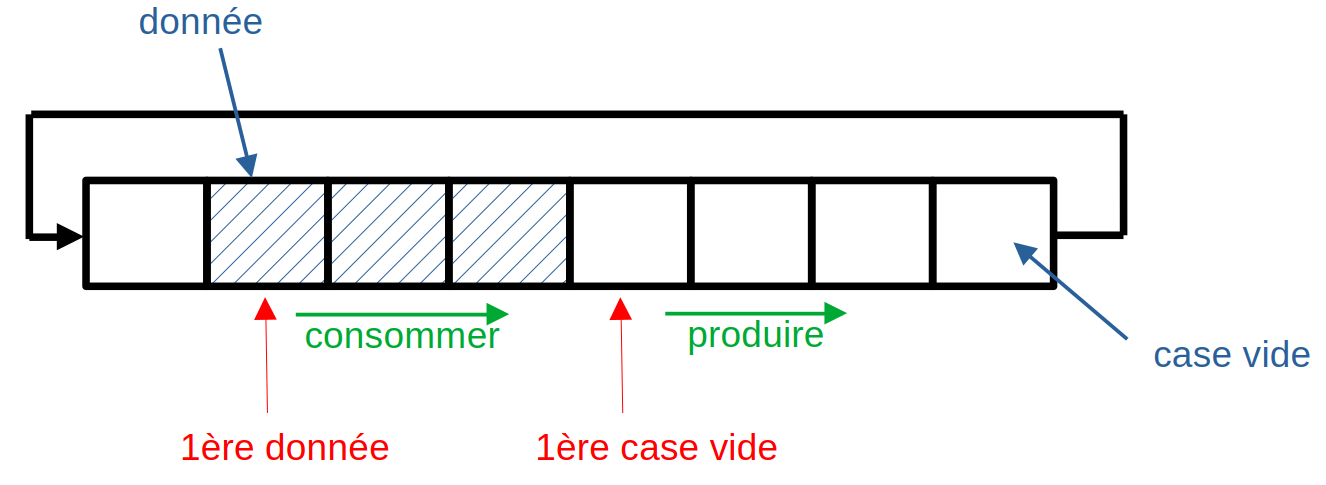
\includegraphics[width=0.7\linewidth]{lecon/18-fil/prod-cons.png}
	\end{center}
	
	\paragraph{Problème :} \begin{itemize}
		\item l'accès au tampon est partagé
		\item les consommateurs doivent attendre qu'une place soir produite
		\item les producteurs doivent attendre que de la place soit libérée dans le tampon.
	\end{itemize}
	
	\paragraph{Solution :} On utilise un sémaphore indiquant le nombre données disponibles et un le nombre de cases disponibles.
	
	\begin{lstlisting}[style=CStyle]
		sem_t mutex, vide, plein;
		sem_init(&mutex, 0, 1);
		sem_init(&vide, 0, N);
		sem_init(&plein, 0, 0);\end{lstlisting}
	
	\begin{minipage}{0.45\textwidth}
		Producteur :
		\begin{lstlisting}[style=Cstyle]
			int item;
			while(1){
				item = produire_item()
				// On attend un place
				sem_wait(&vide);
				sem_wait(&mutex);
				insert_item(item);
				sem_post(&mutex);
				// On la remplie
				sem_post(&plein);
		}\end{lstlisting}
	\end{minipage}\qquad
	\begin{minipage}{0.45\textwidth}
		Consommateur :
		\begin{lstlisting}[style=Cstyle]
			int item;
			while(1){
				// On attend un element
				sem_wait(&plein);
				sem_wait(&mutex);
				item = remove_item();
				sem_post(&mutex);
				// On libere une place
				sem_post(&vide);
				consomer_item(item);
		}\end{lstlisting}
	\end{minipage}
	
\end{appl}

\begin{com}
	Par manque de place, on peut moins s'étendre et ne pas écrire l'algorithme, se contenter de dire qu'on a un sémaphore qui compte les places vides et un les places pleines. (et éventuellement virer le dessin)
\end{com}

\begin{rem}
	On peut implémenter un sémaphore par de l'attente active et des verrous. Donc naturellement, ce qu'apporte souvent les sémaphores, par rapport au verrou, c'est moins d'attente active.
\end{rem}

\begin{com}
	Cette remarque, car si on a des élèves un peu rapide, il pourrait trouver assez facilement des solutions n'utilisant que des verrous, et donc se poserait la question de la pertinence des sémaphores dans ce contexte. L'intérêt des sémaphores vient alors de la suppression de l'attente active.
\end{com}

\section{Interblocage}

\begin{definition}
	On dit qu'il y a interblocage quand tous les fils sont bloqués et ne seront jamais libérés.
\end{definition}

\begin{example} \enspace\\ \normalfont
	\begin{minipage}{0.3\linewidth}
		Fil 1 :
		\begin{lstlisting}[style=CStyle]
			prendre(m1);
			prendre(m2);\end{lstlisting}
	\end{minipage} \quad
	\begin{minipage}{0.3\linewidth}
		Fil 2:
		\begin{lstlisting}[style=CStyle]
			prendre(m2);
			prendre(m1);\end{lstlisting}
	\end{minipage}
\end{example}

\begin{definition}[Diner des philosophes]
	On a cinq philosophes autour d'une table ronde et une fourchette entre chaque. Chaque philosophe alterne moment de faim et de réflexion. Quand il a faim, il attend de prendre ses deux fourchettes, puis il mange, les repose etc.
\end{definition}

\paragraph{Solution naïve :} Un verrou par fourchette, chaque philosopge attend de prendre sa fourchette gauche, puis sa droite

\paragraph{Problème :} Interblocage

\begin{exercise}
	L'implémenter pour observer cet interblocage
\end{exercise}

\paragraph{Solution :} \begin{itemize}
	\item Avec des verrous : chaque philosophe essaye d'abord de prendre sa fourchette de plus petit indice
	\item Avec des sémaphores : On n'autorise que 4 philosophes à essayer de prendre des fourchettes grâce à un sémaphore
\end{itemize}

\begin{com}
	Bon on pourrait aussi mettre dans cette partie un petit dessin.
\end{com}

\chapter{Stockage et manipulation de données, des fichiers aux bases de données.} \label{L21}
\dev{Emile Martinez}{Balabonski, Barra}

La mémoire d'un programme meurt avec lui. Néanmoins, on souhaite garder des données plus perennement.

La mémoire d'un ordinateur est alors une série de milliards de bits, parmi lesquels coexistent tout et n'importe quoi. On veut les organiser de façon à rendre leur accès le plus simple et rapide possible.

\section{Fichiers}

\subsection{Organisation et manipulation}

\begin{definition}
	Un fichier est un ensemble de données. C'est l'unité de stockage manipulé par l'utilisateur.
\end{definition}

\begin{definition}
	Pour organiser des données de manière persistante sur un disque on utilise une arborescence de fichier. La norme POSIX, suivie par la plupart des OS (linux, Mac, android) définit cette organisation et sa manipulation.
\end{definition}

\begin{example}
	Arborescence de fichier linux (obtenue par la commande \texttt{tree})\\
	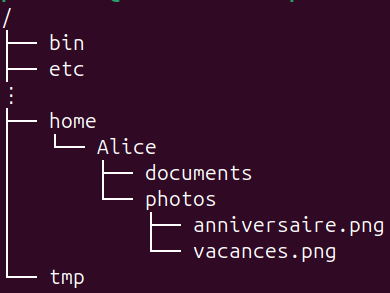
\includegraphics[width=0.4\linewidth]{lecon/21-fichier/arborescence.png}
\end{example}

\begin{definition}
	Le chemin d'accès vers un fichier est soit exprimé de manière absolu (depuis la racine) soit depuis le répertoire courant
\end{definition}

\begin{impl}
	On peut accèder et manipuler l'arborescence de fichier depuis un invite de commande (shell ou terminal) avec les commandes suivantes : \begin{itemize}[label=$\bullet$]
	\item pwd : affiche le repertoire courant
	\item cd chemin : change le repertoire courant pour la cible du chemin
	\item mkdir/touch : créer un dossier/un fichier
	\item cp/mv/rm : copie/ déplace et renomme / supprime
	\item ls  : liste le contenu d'un repertoire
	\end{itemize}
\end{impl}

\begin{exercise}
	Prise en main des commandes du shell avec appuie sur l'utilisation du man.
\end{exercise}

\begin{impl}
	La commande ls -l permet de faire apparaitre des informations supplémentaires sur les fichiers : propriétaire, groupe prioritaire, taille, dernière modification et autorisations :
	\normalfont
	$$ \underset{\circled{1}}{\underbrace{\texttt{\enspace\enspace-}}} \underset{\circled{2}}{\underbrace{\texttt{rwx}}}\underset{\circled{3}}{\underbrace{\texttt{r--}}}\underset{\circled{4}}{\underbrace{\texttt{r--}}}$$
	
	$\circled{1}$ : type de fichier : \begin{itemize}
		\item[] \qquad \texttt{d} : répertoire
		\item[] \qquad \texttt{l} : lien symbolique
		\item[] \qquad \texttt{-} : autre
	\end{itemize}
	
	$\circled{2}\circled{3}\circled{4}$ : \begin{itemize}
		\item[] \qquad \texttt{r} : read
		\item[] \qquad \texttt{w} : write
		\item[] \qquad \texttt{x} : execute
	\end{itemize}
	
	$\circled{2}$ : permissions propriétaire
	
	$\circled{3}$ : permissions groupe
	
	$\circled{4}$ : permissions tous
	
	
\end{impl}

\begin{rem}
	Pour Linux, "tout est un fichier" : les codes sources, les exécutables, mais aussi les périphériques qui peuvent être lus (souris, clavier) ou écrits (écran) comme des fichiers
\end{rem}

\begin{proposition}
	Plusieurs systèmes de fichiers (volume dans la mémoire) peuvent cohabiter sur un même ordinateur, avec chacun leur racine
\end{proposition}

\begin{example}
	Les C::, D::, E::, etc. sous Windows sont autant de système de fichiers
\end{example}

\begin{rem}
	Sous Linux, tous les espaces de stockages montés partagent la même arborescence
\end{rem}

\subsection{Stockage}

Il existe plusieurs manières de faire un système de fichier (FAT32, ext4, \dots) définissant des primitives de gestion des fichiers ainsi que des structures de données pour la gestion des espaces libres.

\begin{definition}
	On découpe alors les fichiers en blocs de quelques ko. Le système de fichier ne manipulera alors que des blocs.
\end{definition}

\begin{definition}
	Un fichier étant souvent trop grand pour un unique bloc, il est séparé en plusieurs blocs : \begin{itemize}
	
	\item allocation contigüe : les blocs sont contigües sur le disque \\
	$\to$ accès séquentiel rapide mais fragmentation et difficulté à créer ou etendre des fichiers.
	
	\item allocation chaînée : les blocs peuvent être n'importe où, chaque bloc contenant l'adresse du suivant\\
	$\to$ bonne utilisation de la mémoire, création extension facile mais accès séquentiel lent
	
	On dispose alors parfois d'une table d'allocation de fichiers
	
	\item l’allocation indexée : les adresses des blocs constituant un même fichier sont rangées dans une table, appelée index, elle-même con
	
	tenue dans un ou plusieurs blocs.
	
	$\to$ bonne accès séquentiel et extension facile, mais taille de fichier maximales et utilisation de mémoire annexe (visible surtout sur les petits fichiers)
	\end{itemize}
\end{definition}


\begin{definition}
	Chaque fichier se voit associé un numéro inode à un emplacement de stockage. L'inode permet de retrouver dans une table du périphérique de stockage des infos données par \texttt{ls -l}.
\end{definition}

\begin{definition}
	Pour économiser de la place, des liens peuventêtre crées entre des fichiers avec :
	
	\qquad \texttt{ln} : lien physique, l'inode est partagé mais la suppression d'un des fichiers n'impacte pas l'autre
	
	\qquad \texttt{ln -s} : lien symbolique, un nouvel inode est utilisé et le fichier ne contient que le chemin vers sa source.

\end{definition}

\section{Format}

\subsection{Fichier texte}

\begin{definition}
	Un fichier texte représente uniquement une suite de caractères (type char en C ou en OCaml) codé en ASCII.
\end{definition}

\begin{rem}
	C'est le format de fichier de base.
\end{rem}

\begin{rem}
	Il arrive que l'on veuille représenter plus que les 128 caractères qu'autorise l'ASCII (ou 256 pour l'ASCII étendue). On peut alors utiliser des codages sur plus de bits (16 pour l'unicode par exemple).
\end{rem}

\begin{definition}
	Étant le format de fichier le plus basique, il est le plus simple à manipuler. On pourra alors accéder à ces fichiers en langage de programmation :\\
	\begin{tabular}{l|l|l}
		\multicolumn{1}{c}{Fonction} & \multicolumn{1}{|c|}{En C} & \multicolumn{1}{c}{En OCaml}\\
		ouvrir un fichier &  \texttt{fopen(chemin, mode)} & \texttt{open\_in} \\
		fermer un fichier & \texttt{fclose(fichier)} & \texttt{close\_in} \\
		écrire dans un fichier & \texttt{fprintf} & \texttt{input\_line} \\
		lire dans un fichier & \texttt{scanf} & \texttt{output\_line}
	\end{tabular}
\end{definition}

\begin{rem}
	Lorsqu'on utilise \texttt{printf} en C, on écrit dans un fichier particulier : la sortie standard (stdout) qui correspond à l'invite de commande. \texttt{printf} est donc équivalent à \texttt{fprintf(stdout, $\dots$)}. De même, \texttt{scanf} lit dans l'entrée standard (stdin). 
\end{rem}

\begin{definition}
	Pour rediriger la sortie standard, on peut utiliser des commandes : \begin{itemize}
		\item \texttt{commande > filename} : la sortie standard de la commande est écrite ddans le fichier, qui est écrasé.
		\item \texttt{commande >> filemane} : même chose mais sans écraser le fichier. 
		\item \texttt{commande < fichier} : le fichier devient l'entrée standard de la commande
		\item \texttt{commande1 | commande2} : la sortie standard de la première commande est reliée à l'entrée standard de la deuxieme.
	\end{itemize}
\end{definition}

\begin{rem}
	L'écriture étant lente, un tampo est utilisé. On peut forcer l'écriture des tampons avec \texttt{flush} en OCaml et \texttt{fflush} en C.
\end{rem}

\subsection{Formats de fichiers}

Pour représenter plus que des chaînes caractères, on a besoin de définir des formats de fichiers qui indiquent comment interpréter les bits de données. 

\begin{definition}
	Un format de fichier est une convention de représentation de données
\end{definition}

\begin{rem}
	Pour gagner de l'espace, ces formats utilisent souvent des méthodes de compression, avec ou sans perte.
\end{rem}

\begin{example}
	Quelques formats particuliers :
	\begin{itemize}
		\item Le format png stocke et compresse les images sans perte
		\item Le format jpeg stocke des images compressées avec perte
		\item Le formats mp3 stocke des sons compressés avec perte
		\item Le format mp4 combine audio et vidéo
		\item Le format zip compresse sans perte des fichiers quelconques
	\end{itemize}
\end{example}

\begin{rem}
	Le format zip utilise l'algorithme de compression LZW, mais aussi le codage de Huffman.
\end{rem}

\paragraph{Développement :} Présentation de l'algorithme LZW.

\begin{rem}
	Il y a toujours un compromis à faire entre différents objectifs (ex : compression et facilité d'utilisation). Ainsi la plupart des formats se spécialisent dans une utilisation :
	\begin{itemize}
		\item quand on ouvre une image en python, on la transforme en tableau de triplets, quand on la sauvegarde on la recompresse, dans un format moins manipulable
		\item Quand on édite une vidéo, on doit l'exporter à la fin pour passer d'un format manipulable à un format pour la lecture
		\item Quand on compresse des fichiers en .zip, on ne peut plus les modifier ou les lire 
	\end{itemize}raison pour lesquelles on exporte quand on monte une vidéo, pour baser d'un format éditable à un format compressé adapté à la lecture).
\end{rem}

\begin{example}
	Le format CSV (pour comma separated values) est un format de texte brut permettant de stocker des données sous forme de table, permettant ainsi facilement la suppresion, l'ajout, etc.\\
	
	Pour des commandes \{ produit : tomate, prix : 3 quantité : 50, client : Le navet naviguant, adresse : 13 rue du Swag à Tarbes \},  \{ produit : patate, prix : 1, quantité : 30, client : Le navet naviguant, adresse : 13 rue du Swag à Tarbes \},  \dots
	
	Pourrait-on mieux faire ?
\end{example}

\section{Bases de données}

Souvent, les données d'une table ont des redondances, et des liens entre elles (cf exemple au dessus). Pour manipuler des gros volumes de données on ne se contente alors plus alors de fichiers en texte brut.

\begin{definition}
	Le modèle relationnel est une manière de représenter les données en exploitant les relations entre elles.
\end{definition}

\begin{example}
	Un grossistes gérant des commandes.
	\normalfont\\
	\texttt{Produit(\underline{num\_produit}, nom, prix, poids)}\\
	\texttt{Clients(\underline{num\_client}, nom, adresse, ville)}\\
	\texttt{Commande(\underline{\#num\_produit, \#num\_client}, quantite)}\\
	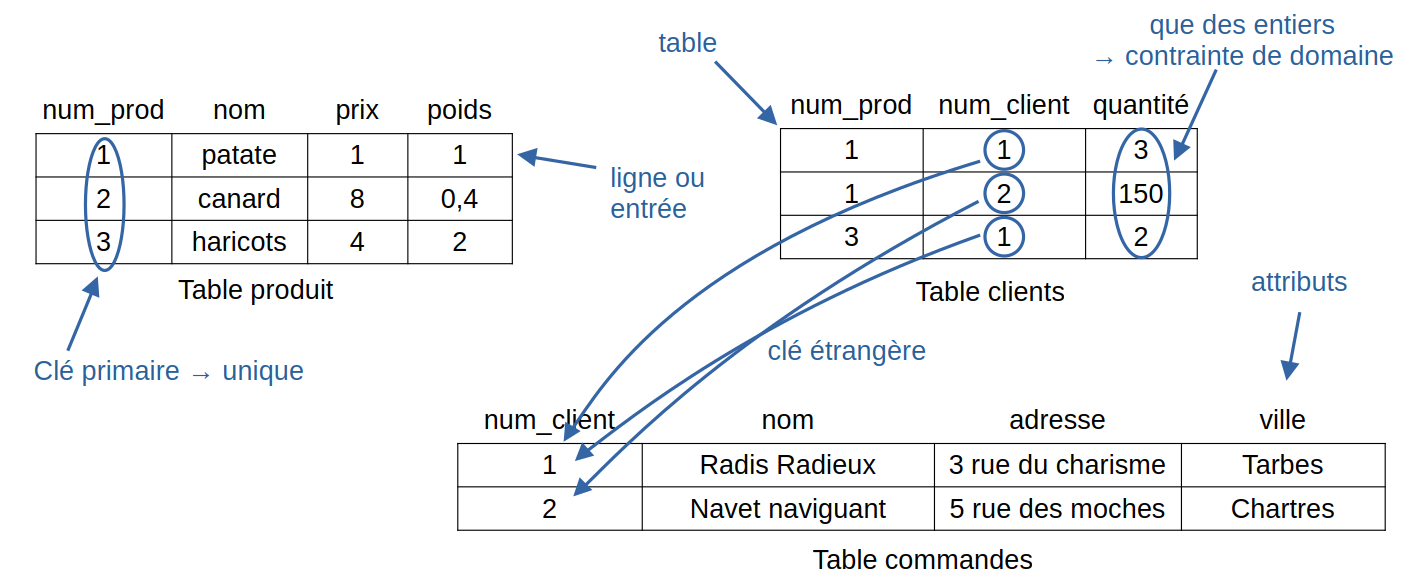
\includegraphics[width=\linewidth]{lecon/21-fichier/schema_bd.png}
\end{example}

\begin{definition}
	Un SGBD (système de gestion de bases de données) est utilisé pour manipuler des données relationnelles, garantissant les propriétés ACID (atomicité, cohérence, isolation et durabilité). On intéragit avec lui à travers le langage SQL.
\end{definition}

\begin{example}
	Le SQL permet de sélectionner certaines données, de les trier, de les filtrer selons certaines conditions, etc \dots
\end{example}

\begin{com}
	Si on a la place ici, on peut insérer des mots clés.
\end{com}

\begin{theorem}[Codd]
	SQL est suffisamment expressif pour quasiment tout ce que l'on souhaite faire
\end{theorem}

\begin{exercise}
	Trouver différentes manières de calculer le max et la division.
\end{exercise}

\paragraph{Développement :} Correction de l'exercice précédent.

\begin{com}
	Ici on pourrait également défendre le fait de faire plutôt l'autre développement de requêtes SQL, introduisant les requêtes, les mots clés de bases, etc. Il s'insère parfaitement dans la leçon, (mieux que ce développement là où il faut justifier que on a introduit aucune syntaxe dans le cours, mais que en vrai ils la connaîtraient), mais c'est un développement moins poussé. Donc on montre moins la puissance de calcul.
\end{com}



\chapter{Fonctions et circuits booléens en architecture des ordinateurs} \label{L22}
\debut{Emile Martinez}{Prépa / Première}{Représentation binaire et pour la première partie : induction, graphe}{}

\section{Cadre théorique (Prépa)}

\subsection{Expression booléenne}

\begin{definition}
	On définit l'ensemble $EB$ des expressions booléennes par induction avec la signature
	\begin{itemize}[label=$\bullet$]
		\item cas de bases : $\top, \,\bot, \,V$ un ensemble de variables
		\item constructeurs :\begin{itemize}[label=$\star$]
			\item $\neg$ un constructeur unaire
			\item $\vee, \, \wedge$ deux constructeurs binaires
		\end{itemize}
	\end{itemize}
\end{definition}

Informellement : $\top, \bot, x \in V$ sont des expressions booléennes, et si $e_1$ et $e_2$ le sont, alors $\neg e_1$, $e_1\vee e_2$, et $e_1 \wedge e_2$ le sont.

\begin{exercise}
	Définir inductivement les variables apparaissant dans une formule et en déduire une définition rigoureuse du nombre de variables d'une fonction.
\end{exercise}

\begin{definition}
	Une valuation est une fonction $\sigma :V \to \{0,1\}$.
	\\
	\\
	On définit alors $[\,]_\sigma$ : $EB \to \{0, 1\}$ par induction sur EB par :\begin{itemize}[label=$\bullet$]
		\item $[\bot]_\sigma = 0$, $[\top]_\sigma = 1$ et $[x]_\sigma = \sigma(x)$ pour $x \in V$
		\item $[e_1 \vee e_2] = \max([e_1]_\sigma, [e_2]\sigma)$
		\item $[e_1 \wedge e_2] = \min([e_1]_\sigma, [e_2]\sigma)$
		\item $[\neg e_1]_\sigma = 1-[e_1]_\sigma$
	\end{itemize}
\end{definition}

\begin{definition}
	Pour $a, b \in EB$, on dit que $a$ et $b$ sont équivalentes noté $a \equiv b$, si $\forall \sigma :V \to \{0,1\}, [a]_\sigma = [b]_\sigma$
\end{definition}

\begin{definition}
	On peut éventuellement définir le XOR (ou exclusif), avec $a\oplus b = (a\vee b)\wedge \neg(a\wedge b) \equiv (a\wedge \neg b)\vee (\neg a\wedge b)$
\end{definition}

\subsection{Fonctions booléennes}

\label{22-1-2}

\begin{definition}
	Une fonction booléenne est une fonction de $\{0, 1\}^n \to \{0, 1\}^m$
\end{definition}

\begin{example}
	$f : \{0,1\}^{64} \to \{0,1\}^{64}$ prenant en entrée le codage (en double) d'un flottant $x$, et renvoyant le codage du flottant de $e^x$
\end{example}

\begin{rem}
	On se limite parfois à $f : \{0,1\}^n \to \{0, 1\}$ (en décomposant $f : \{O, 1\}^n \to \{0, 1\}^m$ en $m$ fonctions sur chaque dimension)
\end{rem}

\begin{definition}[Table de vérité]
	La table de vérité d'une fonction booléenne est la donnée de sa valeur sur toutes ses entrées possibles. On représente la table de vérité de $f:\{0,1\}^n \to \{0,1\}^m$ dans un tableau avec $n+m$ colonnes, et pour chaque éléments de $\{0,1\}^n$, une ligne avec la valeur du $n$-uplets, et la valeur du $m$-uplets de sortie.
\end{definition}

\begin{rem}
	La table a $2^n$ lignes
\end{rem}

\begin{com}
	Bon là normalement il faudrait en mettre une, mais bon, il faut aussi que jeunesse se passe.
\end{com}

\begin{rem}
	On se limite parfois à $f : \{0,1\}^n \to \{0, 1\}$ (en décomposant $f : \{O, 1\}^n \to \{0, 1\}^m$ en $m$ fonctions sur chaque dimension)
\end{rem}

On peut définir une fonction booléenne : \begin{itemize}
	\item par extension (en donnant sa table de vérité)
	\item par intention (en donnant ses propriétés (ex: 1 ssi le nombre de variables à 1 est un nombre premier))
	\item par une expression booléenne.
\end{itemize}

\begin{theorem}
	\label{22-equivalence}
	Toute fonction $f:\{0,1\}^n -> \{0,1\}$ est équivalente à une expression booléenne.
	
	Plus rigoureusement, il existe une formule $e$ dont les variables sont $x_1, \dots, x_n$ et telle que pour toute valuation $\sigma$, $[e]_\sigma = f(\sigma(x_1), \dots, \sigma(x_n))$
\end{theorem}

\par{Développement :} Preuve du théorème \ref{22-equivalence} et discussion sur la complexité.

\subsection{Représentation des expressions booléennes par des graphes orientés acycliques}

\begin{definition}[Circuit booléen]
	Un circuit est un graphe orienté acyclique (DAG) étiquetés par $V \cup \{\top,\bot, \neg, \wedge, \vee \}$ où un sommet d'étiquette $x$ a : \begin{itemize}[label=$\bullet$]
		\item Un degré entrant 0 si $x \in V \cup \{\top, \bot\}$
		\item Un degré entrant 1 si $x = \neg$
		\item Un degré entrant 2 si $x \in \{\wedge, \vee\}$
	\end{itemize}
\end{definition}

\begin{rem}
	On peut ne pas prendre également des étiquettes supplémentaires (comme $\oplus$, le NAND, NOR, etc.)
\end{rem}

\begin{definition}
	On définit l'évaluation d'un graphe par une valuation $\sigma :V \to \{0,1\}$ comme un étiquetage des nœuds où un nœud d'étiquette $a$ vaudra : \begin{itemize}[label=$\bullet$]
		\item $[a]_\sigma$ si $a \in V \cup \{\top, \bot\}$
		\item $1-y$ si $a = \neg$ et le sommet entrant de $a$ est évalué en $y$
		\item $\min(y, z)$ (resp. $\max(y, z)$) si $a= \wedge$ (reps.$\vee$) et les sommets entrants sont évalués en $y$ et $z$
	\end{itemize}
\end{definition}

\begin{proposition}
	Cette définition est correcte (et ne boucle pas à l'infini)
\end{proposition}

\begin{rem}
	\begin{itemize}[label=$\bullet$]
		\item Les degrés sortants ne sont pas limités.
		\item Si les degrés sortants sont exactement 1 sauf pour un sommet où c'est 0, on obtient exactement les expressions booléennes (avec leur représentation sous forme d'arbres)
		\item Les circuits booléens correspondraient à un ensemble d'expressions booléennes où l'on aurait le droit de définir des alias
	\end{itemize}
\end{rem}

\begin{personalise}[Conclusion]
	Les circuits booléens peuvent représenter tout ce qu'on veut calculer de finis et qu'on peut coder en binaire.
\end{personalise}

\section{Dans un ordinateur}

\subsection{Circuits combinatoires}

\begin{definition}
	Un bit est la plus petite unité d'information d'un ordinateur, ne pouvant prendre que deux valeurs (0V - +5V, 0 - 1, Ying - Yang, Ouvert - Fermé, \dots). Fixons nous sur 0-1.
\end{definition}

Dans les circuits électroniques, on arrive à manipuler des bits. Nous sommes par exemples capables de prendre un bit et de l'inverser, d'en prendre deux et de renvoyer 1 si au moins l'un des deux vaut 1, etc\dots

\begin{definition}[porte logique]
	Une porte logique est un circuit électronique réalisant des opérations logiques sur une séquence de bits
\end{definition}

\begin{example}
	On est capable de faire les portes ET, OU, NON, \dots\\
	\begin{tabular}{ccc}
		\begin{circuitikz} \draw
			(0,0) node[and port] (a) {}
			;  
		\end{circuitikz} & \begin{circuitikz} \draw
		(0,0) node[or port] (a) {}
		;  
		\end{circuitikz} & \begin{circuitikz} \draw
		(0,0) node[not port] (a) {}
		;  
		\end{circuitikz} \\
		ET & OU & NON
	\end{tabular}
\end{example}

\begin{definition}[circuits combinatoires]
	Un circuit combinatoire est alors une succession de portes logiques dont la sortie de certaines sont branchés sur l'entrée d'autres, et sans cycles.
\end{definition}

\begin{rem}
	C'est l'implémentation physique des circuits booléens.
\end{rem}

\begin{personalise}[Conclusion]
	Les parties I-II, I-III et II-I nous donnent que l'on est capable électroniquement de calculer tous qui est représentable de manière fini par des bits.
\end{personalise}

\section{Mesure d'un circuit}

\begin{idee}
	Quand on fait un circuit booléens, on peut vouloir maximiser différents critères : \begin{itemize}[label=$\bullet$]
		\item On veut, pour des raisons économiques, minimiser le nombre de transistors (et donc le nombre de portes)
		\item On veut tirer des câbles courts, et donc avoir un circuit compact
		\item Comme il y a un délai pour qu'une porte calcule sa sortie selon son entrée, on veut minimiser le délai total de mise à jour du circuit.
	\end{itemize}
\end{idee}

\begin{definition}[chemin critique]
	Le chemin critique d'un circuit booléen (et donc d'un circuit combinatoire) est le (un) plus long chemin entre une entrée (degré entrant 0) et une sortie (degré sortant  0). Le graphe étant acyclique, c'est donc un plus long chemin.
\end{definition}

\begin{idee}
	Minimiser la longueur du chemin critique, qui est proportionnelle au délai que met un circuit combinatoire à effectuer un calcul.
\end{idee}

\begin{example}
	$a \oplus b \oplus c$ peut-être représenté par deux XOR successifs \\
	% les dessins ici sont plus ou moins exportées depuis https://circuit2tikz.tf.fau.de/designer/
	\begin{tikzpicture}
		% Paths, nodes and wires:
		\draw node[american and port, red] at (5.136, 8.22) {};
		\draw node[american and port] at (5.136, 6.28) {};
		\draw node[ieeestd not port] at (2.877, 6) {};
		\draw node[ieeestd not port, red] at (2.873, 7.94) {};
		\draw node[circ] (N1) at (0.25, 8.5) {} node[anchor=east] at (N1.text){$a$};
		\draw node[circ] (N2) at (0.25, 5.31) {} node[anchor=east] at (N2.text){$c$};
		\draw[draw] (0.25, 8.5) -- (3.75, 8.5);
		\draw[draw] (1, 8.5) -| (1.25, 6) -- (2, 6);
		\draw[draw] (3.75, 6.56) -| (1.996, 7.94);
		\draw node[circ] (N3) at (0.25, 7.94) {} node[anchor=east] at (N3.text){$b$};
		\draw node[american or port, red] at (7.75, 7.25) {};
		\draw[draw] (5.29, 6.28) -| (6.364, 6.97);
		\draw node[american and port] at (12.79, 6.97) {};
		\draw node[american and port, red] at (12.79, 5.03) {};
		\draw node[ieeestd not port, red] at (10.531, 4.75) {};
		\draw node[ieeestd not port] at (10.527, 6.69) {};
		\draw[draw] (7.904, 7.25) -- (11.404, 7.25);
		\draw node[american or port, red] at (15.404, 6) {};
		\draw[draw] (12.944, 6.97) -| (14.018, 6.28);
		\draw[draw] (11.404, 5.31) -| (9.65, 6.69) |- (0.25, 5.31);
		
		
		%draw critical path
		\draw[draw, red] (1.996, 7.94) -| (0.25, 7.94);
		\draw[draw, red] (5.29, 8.22) -| (6.364, 7.53);
		\draw[draw, red] (7.904, 7.25) -| (8.904, 4.75) -- (9.654, 4.75);
		\draw[draw, red] (12.944, 5.03) -| (14.018, 5.72);
	\end{tikzpicture}\\
	On a alors 10 portes et un chemin critique de taille 6. On peut le diminuer à 5, en calculant directement la négation de $a \oplus b$, au lieu de réutiliser le résultat de $a \oplus b$
	
	
	\noindent \begin{tikzpicture}
		% Paths, nodes and wires:
		\draw node[american and port] at (5.136, 8.22) {};
		\draw node[american and port] at (5.136, 6.28) {};
		\draw node[ieeestd not port] at (2.873, 7.94) {};
		\draw node[circ] (N1) at (0.25, 8.5) {} node[anchor=east] at (N1.text){$a$};
		\draw node[circ] (N2) at (0.25, 5.25) {} node[anchor=east] at (N2.text){$c$};
		\draw[draw] (0.25, 8.5) -- (3.75, 8.5);
		\draw[draw] (1, 8.5) -| (1.25, 6) -- (2, 6);
		\draw[draw] (3.75, 6.56) -| (1.996, 7.94) -| (0.25, 8);
		\draw node[circ] (N3) at (0.25, 7.94) {} node[anchor=east] at (N3.text){$b$};
		\draw node[american or port] at (7.75, 7.25) {};
		\draw[draw] (5.29, 8.22) -| (6.364, 7.53);
		\draw[draw] (5.29, 6.28) -| (6.364, 6.97);
		\draw node[american and port] at (11.763, 6.97) {};
		\draw node[ieeestd not port] at (9.5, 6.69) {};
		\draw[draw] (7.904, 7.25) -- (10.377, 7.25);
		\draw node[american or port] at (13.886, 8.78) {};
		\draw node[ieeestd not port] at (2.877, 6) {};
		\draw[draw] (0.25, 5.25) -| (8.623, 6.69);
		\draw node[ieeestd not port] at (2.127, 10.94) {};
		\draw node[ieeestd not port] at (2.127, 9.69) {};
		\draw[draw] (3, 10.94) -| (3.75, 10.5);
		\draw[draw] (3.004, 9.69) -| (3.75, 9.94);
		\draw node[american and port] at (5.136, 10.22) {};
		\draw[draw] (0.75, 8.5) |- (1.25, 10.94);
		\draw[draw] (1.25, 9.69) -| (1, 8) |- (0.613, 7.938);
		\draw node[american and port] at (5.136, 12.03) {};
		\draw[draw] (3.75, 12.31) -| (0.75, 12.25) -- (0.75, 10.94);
		\draw[draw] (3.75, 11.75) |- (1, 11.75) -- (1, 9.69);
		\draw node[american or port] at (7.75, 11.25) {};
		\draw[draw] (5.29, 12.03) -| (6.364, 11.53);
		\draw[draw] (5.29, 10.22) -| (6.364, 10.97);
		\draw node[american and port] at (11.75, 10.5) {};
		\draw[draw] (8.623, 6.69) |- (10.364, 10.22);
		\draw[draw] (10.364, 10.78) -| (8.5, 11) |- (7.904, 11.25);
		\draw[draw] (11.904, 10.5) -| (12.5, 9.06);
		\draw[draw] (11.917, 6.97) -| (12.5, 8.5);
	\end{tikzpicture}\\
	Néanmoins, on a maintenant 14 portes.
\end{example}

\begin{com}
	Cet exemple sur un exemple non trivial le fait que on peut raccourci le chemin critique, et le fait que on peut le faire potentiellement au détriment du nombre de noeuds. (il faut voir le deuxième comme le premier, sauf qu'on calcule directement la négation du xor). Mais bon, cet exemple est un peu gros à mettre dans le plan quoi. Si on veut un truc plus cours, on peut passer de $a \wedge (b \vee c) \wedge d$ à $(a \wedge d) \wedge (b \vee c)$ mais on rajoute pas de portes, et cet exemple est bateau et donc moins intéressant que le XOR ternaire. Mais bon, il faut savoir vivre avec son temps.
\end{com}


\section{Des circuits particuliers}

\subsection{Additionneur n bits}

\begin{algo}
	On reprend l'algorithme classique d'addition, adapté au binaires :\\
	\begin{algorithm}[H]
		\caption{$Addition(x, y)$}
		\Entree{$x$ et $y$ deux nombres de $n$ chiffres en binaire}
		$r_{-1} \gets 0$\\
		\Pour{$i = 0$ à $n-1$}
		{
			\tcp{$r_i$ est la $i$-ème retenue, $s_i$ le $i$-ème bit de sortie}
			$r_i, s_i = AC(r_{i_1}, x_i, y_i)$
		}
	\end{algorithm}
	avec AC (additionneur complet) faisant l'addition de trois chiffres (0 ou 1) définie par la table de vérité :\\
	\begin{tabular}{|c|c|c||c|c|}
		\hline
		$r_{i-1}$ & $x_i$ & $y_i$ & $r_i$ & $s_i$  \\ \hline
		0 & 0 & 0 & 0 & 0 \\ \hline
		0 & 0 & 1 & 0 & 1 \\ \hline
		0 & 1 & 0 & 0 & 1 \\ \hline
		0 & 1 & 1 & 1 & 0 \\ \hline
		1 & 0 & 0 & 0 & 1 \\ \hline
		1 & 0 & 1 & 1 & 0 \\ \hline
		1 & 1 & 0 & 1 & 0 \\ \hline
		1 & 1 & 1 & 1 & 1\\ \hline
	\end{tabular} \quad que l'on représente par \qquad \raisebox{-0.5\height}{\begin{tikzpicture}[->, node distance=0.3cm]
		\node[rectangle, draw] (ac) {\quad$\substack{\\\\\\AC\\\\\\}$\enspace\enspace};
		
		\node[above left = 0.5cm and -0.7cm of ac] (xi) {$x_i$};
		\node[below = 0.5cm of xi] (xi-faux) {};
		\draw (xi) edge[] (xi-faux);
		
		\node[above right = 0.5cm and -0.7cm of ac] (yi) {$y_i$};
		\node[below = 0.5cm of yi] (yi-faux) {};
		\draw (yi) edge[] (yi-faux);
		
		\node[right = 0.5cm of ac] (ri-1) {$r_{i-1}$};
		\node[left = 0.5cm of ri-1] (ri-1-faux) {};
		\draw (ri-1) edge[] (ri-1-faux);
		
		\node[left = 0.5cm of ac] (ri) {$r_i$};
		\node[right = 0.5cm of ri] (ri-faux) {};
		\draw (ri-faux) edge[] (ri);
		
		\node[below = 0.5cm of ac] (si) {$s_i$};
		\node[above = 0.5cm of si] (si-faux) {};
		\draw (si-faux) edge[] (si);
		
	\end{tikzpicture}}
	
\end{algo}

\begin{exercise}
	Proposer un circuit booléen pour cette table.
\end{exercise}

En mettant plusieurs AC à la suite, on créer alors un additionneur $n$ bits : \begin{center}
	\begin{tikzpicture}[->]
		\node[rectangle, draw] (acn) {\quad$\substack{\\\\\\AC\\\\\\}$\enspace\enspace};
		
		\node[above left = 0.5cm and -0.7cm of acn] (xn) {$x_{n-1}$};
		\node[below = 0.5cm of xn] (xn-faux) {};
		\draw (xn) edge[] (xn-faux);
		
		\node[above right = 0.5cm and -0.7cm of acn] (yn) {$y_{n-1}$};
		\node[below = 0.5cm of yn] (yn-faux) {};
		\draw (yn) edge[] (yn-faux);
		
		\node[right = 0.5cm of acn] (rn-1) {$r_{n-2}$};
		\node[left = 0.5cm of rn-1] (rn-1-faux) {};
		\draw (rn-1) edge[] (rn-1-faux);
		
		\node[left = 0.5cm of acn] (rn) {$r_{n-1}$};
		\node[right = 0.5cm of rn] (rn-faux) {};
		\draw (rn-faux) edge[] (rn);
		
		\node[below = 0.5cm of acn] (sn) {$s_{n-1}$};
		\node[above = 0.5cm of sn] (sn-faux) {};
		\draw (sn-faux) edge[] (sn);
		
		\node[right = 1cm of rn-1] (points) {. . .};
		
		
		\node[rectangle, draw, right = 2cm of points] (ac1) {\quad$\substack{\\\\\\AC\\\\\\}$\enspace\enspace};
		
		\node[above left = 0.5cm and -0.7cm of ac1] (x1) {$x_1$};
		\node[below = 0.5cm of x1] (x1-faux) {};
		\draw (x1) edge[] (x1-faux);
		
		\node[above right = 0.5cm and -0.7cm of ac1] (y1) {$y_1$};
		\node[below = 0.5cm of y1] (y1-faux) {};
		\draw (y1) edge[] (y1-faux);
		
		\node[right = 0.5cm of ac1] (r0) {};
		\node[left = 0.5cm of r0] (r0-faux) {};
		
		\node[left = 0.5cm of ac1] (r1) {$r_1$};
		\node[right = 0.5cm of r1] (r1-faux) {};
		\draw (r1-faux) edge[] (r1);
		
		\node[below = 0.5cm of ac1] (s1) {$s_1$};
		\node[above = 0.5cm of s1] (s1-faux) {};
		\draw (s1-faux) edge[] (s1);
		
		
		\node[rectangle, draw, right= 0cm of r0] (ac0) {\quad$\substack{\\\\\\AC\\\\\\}$\enspace\enspace};
		
		\draw (ac0) edge[above] node{$r_0$} (r0-faux);
		
		\node[above left = 0.5cm and -0.7cm of ac0] (x0) {$x_0$};
		\node[below = 0.5cm of x0] (x0-faux) {};
		\draw (x0) edge[] (x0-faux);
		
		\node[above right = 0.5cm and -0.7cm of ac0] (y0) {$y_0$};
		\node[below = 0.5cm of y0] (y0-faux) {};
		\draw (y0) edge[] (y0-faux);
		
		\node[right = 0.5cm of ac0] (r-1) {$r_{-1} = 0$};
		\node[left = 0.5cm of r-1] (r-1-faux) {};
		\draw (r-1) edge[] (r-1-faux);
		
		\node[below = 0.5cm of ac0] (s0) {$s_0$};
		\node[above = 0.5cm of s0] (s0-faux) {};
		\draw (s0-faux) edge[] (s0);
		
	\end{tikzpicture}
\end{center}

\begin{personalise}[Problème]
	Le chemin critique est linéaire en $n$ (car il faut propager la retenue).
\end{personalise}


\paragraph{Développement :} Construction par une méthode D\&R d'un additionneur $n$ bits à retenue anticipée.

\subsection{Multiplexeur}

\begin{definition}
	Un multiplexeur à deux entrées est un circuit booléen servant à sélectionner une entrée. Une troisième entrée de contrôle, determine si la sortie sera la première ou la deuxième entrée.\\
	
	On lui associe la table de vérité \begin{tabular}{|c|c|c||c|}
		\hline
		$e_0$ & $e_1$ & $c$ & $s$  \\ \hline
		0 & 0 & 0 & 0 \\ \hline
		0 & 0 & 1 & 0 \\ \hline
		0 & 1 & 0 & 0 \\ \hline
		0 & 1 & 1 & 1 \\ \hline
		1 & 0 & 0 & 0 \\ \hline
		1 & 0 & 1 & 1 \\ \hline
		1 & 1 & 0 & 1 \\ \hline
		1 & 1 & 1 & 1 \\ \hline
	\end{tabular} \quad ($s = (c \wedge e_0) \vee (\neg c \wedge e_1)$)\\
	représenté par \raisebox{-0.5\height}{\begin{tikzpicture}[->]
			\node[trapezium, draw, shape border rotate=270, scale=4] (m) {};
			
			\node[above left = -0.3cm and 0.5cm of m] (e0) {$e_0$};
			\node[right = 0.5cm of e0] (e0-faux) {};
			\draw (e0) edge[] (e0-faux);
			
			\node[below left = -0.3cm and 0.5cm of m] (e1) {$e_1$};
			\node[right = 0.5cm of e1] (e1-faux) {};
			\draw (e1) edge[] (e1-faux);
			
			\node[below = 0.7cm of m] (c) {$c$};
			\draw (c) edge[] (m);
			
			\node[right = 0.5cm of m] (s) {$s$};
			\draw (m) edge[] (s);
	\end{tikzpicture}}
\end{definition}

\begin{exercise}
	Construire un circuit booléen pour le multiplexeur à deux entrées.
\end{exercise}

\begin{rem}
	En combinant les multiplexeurs à deux entrées, on peut générer des multiplexeurs à $2^k$ entrées.
\end{rem}

\begin{example}[Multiplexeur à 4 entrées] \\
	\begin{tikzpicture}[->]
		\node[trapezium, draw, shape border rotate=270, scale=4] (m2) {};
		
		\node[above left = -0.3cm and 0.5cm of m2] (e2) {$e_2$};
		\node[right = 0.5cm of e2] (e2-faux) {};
		\draw (e2) edge[] (e2-faux);
		
		\node[below left = -0.3cm and 0.5cm of m2] (e3) {$e_3$};
		\node[right = 0.5cm of e3] (e3-faux) {};
		\draw (e3) edge[] (e3-faux);
		
		
		\node[trapezium, draw, below = 2cm of m2, shape border rotate=270, scale=4] (m1) {};
		
		\node[above left = -0.3cm and 0.5cm of m1] (e0) {$e_0$};
		\node[right = 0.5cm of e0] (e0-faux) {};
		\draw (e0) edge[] (e0-faux);
		
		\node[below left = -0.3cm and 0.5cm of m1] (e1) {$e_1$};
		\node[right = 0.5cm of e1] (e1-faux) {};
		\draw (e1) edge[] (e1-faux);
		
		\node[trapezium, draw, below right = 1cm and 2cm of m2, shape border rotate=270, scale=4] (m3) {};
	
		\node[above left = -0.3cm and 0.5cm of m3] (e4) {};
		\node[right = 0.5cm of e4] (e4-faux) {};
		
		\node[below left = -0.3cm and 0.5cm of m3] (e5) {};
		\node[right = 0.5cm of e5] (e5-faux) {};
		
		\node[right = 0.5cm of m3] (s) {$s$};
		\draw (m3) edge[] (s);
		
		\node[below = 1cm of m1] (c0) {$c_0$};
		\node[right = 2.5cm of c0] (c1) {$c_1$};

		%maintenant il faut tracer tous les traits à la con
		
		\node[above = 0.5cm of c0, minimum size = 0, inner sep=0] (i1) {};
		\node[right = 0.7cm of i1, minimum size = 0, inner sep=0] (i2) {};
		\node[above = 3.5cm of i2, minimum size = 0, inner sep=0] (i3) {};
		\node[left = 0.7cm of i3, minimum size = 0, inner sep=0] (i4) {};
		
		
		\node[right = 1cm of m1, minimum size = 0, inner sep=0] (i5) {};
		\node[right = 1cm of m2, minimum size = 0, inner sep=0] (i6) {};
		
		\draw (c0) edge[] (m1);
		\draw (c1) edge[] (m3);
		
		\draw (c0) -- (i1) -- (i2) -- (i3) -- (i4) -> (m2);
		
		\draw (m1) -- (i5) |- (e5-faux);
		\draw (m2) -- (i6) |- (e4-faux);

	\end{tikzpicture}
\end{example}

\begin{rem}
	Si on interprète $c_1c_0$ comme un nombre en binaire, sa valeur correspond à l'entrée sélectionné.
\end{rem}

\begin{appl}
	On peut alors créer un sélectionneur d'adresse avec un chemin critique de taille $O(\log n)$ ce qui est optimal.
\end{appl}

\begin{com}
	Là si on a la place, pour insister sur l'aspect archi de la leçon, on peut parler plus longuement de cette application, en disant qu'on en met en parralèle pour avoir plus de données, qu'on le fait sur plus de bits d'adresse, sur le fait qu'on utilise qu'un nombre linéaire de portes.
\end{com}

\begin{exercise}
	Faire un démultiplexeur à $2^k$ entrées.
\end{exercise}













\chapter{Principes de fonctionnement des ordinateurs : architecture, notions d’assembleur.} \label{L23}
\debut{Emile Martinez}{}{Représentation des nombres en binaires}{}

\section{Circuits booléens}

\subsection{Porte logique}

Les circuits d'un ordinateur manipulent des bits qui correspondent en interne à des tensions électriques. 


\begin{definition}
	Une porte logique est une fonction qui prend un ou plusieurs bits en entrée et qui renvoie un bit en sortie. 
\end{definition}

\begin{personalise}[Schéma]
	\begin{tabular}{ccc}
		\begin{circuitikz} \draw
			(0,0) node[and port] (a) {}
			;  
		\end{circuitikz} & \begin{circuitikz} \draw
			(0,0) node[or port] (a) {}
			;  
		\end{circuitikz} & \begin{circuitikz} \draw
			(0,0) node[not port] (a) {}
			;  
		\end{circuitikz} \\
		ET & OU & NON
	\end{tabular}
\end{personalise}

\begin{proposition}
	On peut composer les portes logiques, et scinder un fil : on crée alors des circuits booléens. Attention, on ne doit pas créer de boucles dans les circuits.
\end{proposition}

\begin{exercise}
	Exprimer la porte OU à l'aide des portes NON et ET.
\end{exercise}

\subsection{Expressivité}

\begin{definition}
	On définit inductivement l'ensemble EB des expressions booléennes par :
	\begin{itemize}[label=]
		\item Cas de base : $\top, \bot, x\in V$ (où $V$ est un ensemble de variable)
		\item Constructeurs : $\neg$ unaire, $\wedge$ et $\vee$ binaires
	\end{itemize}
\end{definition}

\begin{rem}
	Cela représente exactement les circuits booléens, où seuls les fils initiaux peuvent être dupliqués
\end{rem}

\begin{definition}
	Une valuation est une fonction $\sigma :V \to \{0,1\}$.
	\\
	\\
	On définit alors $[\,]_\sigma$ : $EB \to \{0, 1\}$ par induction sur EB par :\begin{itemize}[label=$\bullet$]
		\item $[\bot]_\sigma = 0$, $[\top]_\sigma = 1$ et $[x]_\sigma = \sigma(x)$ pour $x \in V$
		\item $[e_1 \vee e_2] = \max([e_1]_\sigma, [e_2]\sigma)$
		\item $[e_1 \wedge e_2] = \min([e_1]_\sigma, [e_2]\sigma)$
		\item $[\neg e_1]_\sigma = 1-[e_1]_\sigma$
	\end{itemize}
\end{definition}

\begin{rem}
	Cela revient à simuler l'exécution d'un circuit booléen.
\end{rem}

\begin{theorem}
	Pour toute fonction $f : \{0, 1\}^n \to \{0, 1\}$, il exsite une expression booléenne e ayant pour variables $\{x_1, \dots, x_n\}$ tel que pour tout $(b_1, \dots, b_n)\in\{0,1\}^n$, en prenant $\sigma$ tel que $\sigma(x_i) = b_i$ on ait alors $[e]_\sigma = f(b_1, \dots, b_n)$
\end{theorem}

\paragraph{Développement :} Preuve du théorème précédent et discussion autour de la complexité

\begin{personalise}[Conclusion]
	Les circuits booléens permettent d'exprimer toutes les fonctions que l'on pourrait vouloir calculer
\end{personalise}

\subsection{Introduction du temps}

Notre ordinateur est donc composé de circuits booléens. Néanmoins, on voudrait pouvoir brancher les circuits booléens entre eux (ce qui posent problème car les portes logiques ne changent pas de valeurs instantanément) et avoir de la rétroaction (ce qui est interdit).

\begin{idee}
	On introduit alors des briques de mémoire dans un ordinateur (registre) et une horologe (un tic tac). Les liens entre les différentes circuits ne se font alors que à travers des registres, qui se mettent à jour en même temps grâce à l'horologe. Ainsi, on a jamais de réelles boucles.
\end{idee}

\begin{rem}
	Les registres sont les plus petites unités de mémoire d'un ordinateur.
\end{rem}

\begin{example}
	Compteur sur 8 bits, faisant +1 à chaque tac du tic tac. \raisebox{-0.5\height}{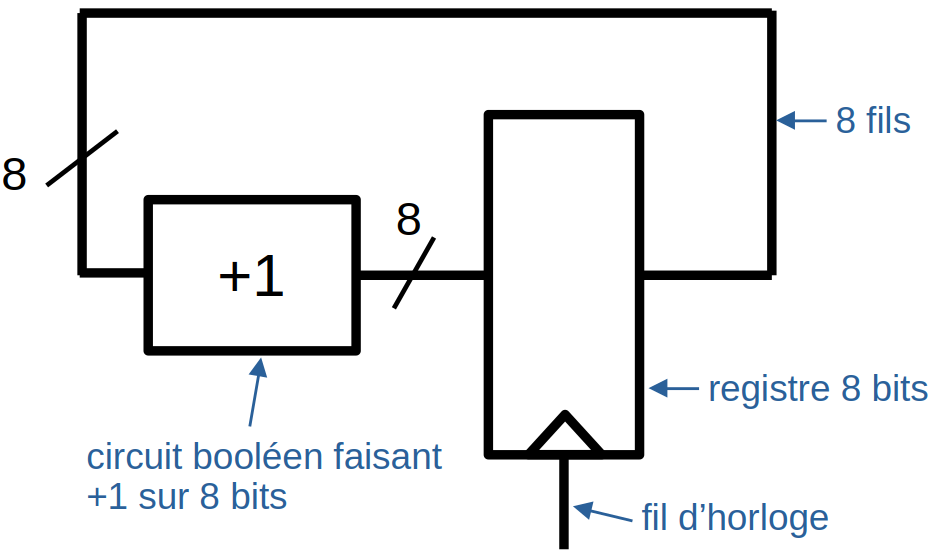
\includegraphics[width=0.4\linewidth]{lecon/23-archi-assembleur/compteur.png}}
\end{example}

\begin{rem}
	La fréquence de l'horloge détermine donc le temps minimal pour faire une opération dans un ordinateur. C'est ce que l'on dit quand on parle de processeur 4GHz (4 milliards de tac par secondes)
\end{rem}

\section{Modèle de Von Neuman}

\subsection{Le modèle}

\begin{definition}
	Une instruction est une opération à effectuer par le processeur sur des éléments de mémoire de l'ordinateur (registre, cache, RAM, disque dur, etc...).
\end{definition}

\begin{principe}
	Un ordinateur passe alors son temps à exécuter des instructions (qui modifie l'état de la mémoire)
\end{principe}

\begin{definition}
 	Le modèle de Von Neumann décrit le fonctionnement d'un ordinateur constitué : \begin{itemize}[label=$\bullet$] 
		\item d'un processeur qui lit les instructions en mémoire et les exécute. Il accède à la mémoire par blocs appelés mots mémoire. Pour cet accès, le processeur utilise un registre appelé compteur ordinal (Program Counter ou PC) qui contient une adresse en mémoire.
		\item La mémoire RAM adressé qui contient les programme à exécuter et les données. 
		\item Les périphériques d'entrée (clavier, souris, disque dur) et de sortie (écran, disque dur, haut parleur).
	 \end{itemize}
\end{definition}

\begin{rem}
	Une des spécificités de ce modèle est que les instructions sont des données comme les autres.
\end{rem}

\begin{personalise}[Schéma][Modèle de Von Neumann] CPU = processeur
	\begin{center}
		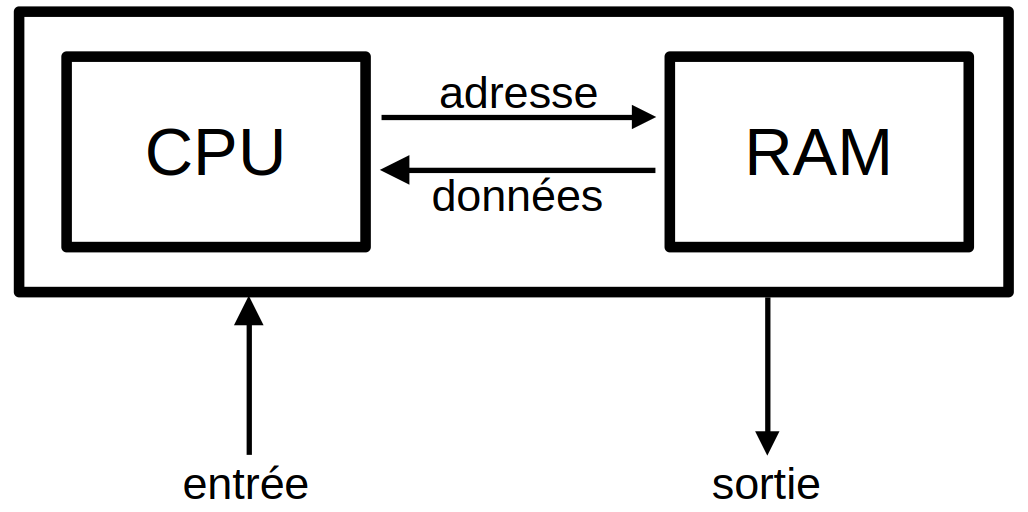
\includegraphics[width=0.5\linewidth]{lecon/23-archi-assembleur/modele_neumann.png}
	\end{center}
\end{personalise}

\begin{definition}[Cylce de Von Neumann]
	\begin{enumerate}
		\item \label{23-point1-cycle} Lire le mot mémoire qui commence à l'adresse PC
		\item Interpréter ce mot mémoire comme une instruction et l'exécuter
		\item Augmenter le PC pour passer à l'instruction suivante
		\item Retourner au \ref*{23-point1-cycle}
	\end{enumerate}
\end{definition}

\begin{rem}
	Quand vous avez plusieurs coeurs, il y a simplement plusieurs processeurs en parrallèle.
\end{rem}

\subsection{Registres et mémoire adressable}

Dans le modèle, la mémoire n'est pas dans le processeur. C'est la mémoire adressable (accessible par adresse).\\

Néanmoins, il y a aussi de la mémoire dans le processeur. Ce sont les registres. Quand un processeur veut exécuter une opération, il doit alors stocker les données dans des registres (les avoir en mémoire, sous la main), faire l'opération (et comme il doit stocker le résultat, le mettre dans un registre), puis renvoyer le résultat à la mémoire.

\begin{rem}
	Un processeur possède un registre stockant la valeur de PC.
\end{rem}

\section{Jeu d'instruction}

\subsection{Définition}

\begin{definition}
	Une instruction machine est une séquence de bits que le processeur peut interpréter et exécuter. Un jeu d'instructions (ISA) définit quelles sont les instructions supportées par le processeur, et la façon dont elles sont représentées en mémoire. L'ensemble de ces instructions machines forment le langage reconnu par le processeur, appelé langage machine. 
\end{definition}

\begin{rem}
	Tous les codes dans n'importe quel langage de programmation (exemple Python) doivent être traduits en langage machine pour être exécutés par le processeur. 
\end{rem}

\begin{proposition}
	En général, les jeux d'instructions gèrent les opérations suivantes : \begin{itemize}[label=$\bullet$]
		\item lire le contenu d'une case mémoire dans un registre, écrire le contenu d'un registre dans une case mémoire 
		\item opérations arithmétiques ou logiques (addition, et bit à bit, etc...)
		\item se déplacer dans le programme que l'on exécute (sauts)
	\end{itemize}
\end{proposition}

\begin{rem}
	Il exsite de nombreux ISA différents. On peut les diviser en deux catégories principales :
	
	CISC (complex instruction set computer) : plus d'instruction pouvant faire plus de choses mais donc plus longues (ex. x86 sur la plupart des ordinateurs)
	
	RISC (reduced instruction set computer) : moins d'instruction mais plus rapide et facile à implémenter (ex : RISC-V, ARM sur des téléphones).
\end{rem}

\subsection{Langage assembleur}

Une instruction est représentée en mémoire par un code en binaire. Par exemple, si les trois premiers bits sont des 0, on doit faire une opération arithmétique, puis si les deux suivants sont des 1, on fait une addition, etc. Néanmoins, cela est très peu lisible par l'être humain.

\begin{definition}
	Le langage assembleur représente le langage machine sous une forme lisible par un humain. C'est le langage de programmation de plus bas niveau.
\end{definition}

\begin{example}
	Exemple d'instruction classique : \begin{itemize}[label=$\bullet$]
		\item \texttt{load $r_i$ [$r_j$]}  : mets le contenu à l'addresse contenu dans $r_j$ dans le registre $r_i$
		\item \texttt{store $r_i$ [$r_j$]} : mets le contenu du registre $r_i$ dans la case d'adresse contenu dans $r_j$
		\item \texttt{add $r_i$ $r_j$ $r_k$} : ajoute le contenu des registres $r_i$ et $r_j$ pour le mettre dans le registre $r_k$
		\item \texttt{iload $r_i$ $x$} : mets la valeur $x$ dans le registre $r_i$
		\item \texttt{mv $r_i$ $r_j$} : mets la valeur du registre $r_i$ dans le registre $r_j$.
	\end{itemize}
\end{example}

\begin{example}
	Traduction en langage assembleur du code python «\texttt{z = x + y}»
	\begin{lstlisting}
iload <@$r_1$@> <@(adresse de x)@>
load <@$r_2$@> [<@$r_1$@>]
iload <@$r_1$@> <@(adresse de y)@>
load <@$r_3$@> [<@$r_1$@>]
add <@$r_1$@> <@$r_2$@> <@$r_3$@>
iload <@$r_1$@> <@(adresse de z)@>
store <@$r_2$@> [<@$r_1$@>]
	\end{lstlisting}
\end{example}

\begin{rem}
	Pour pouvoir exécuter des boucles et les si, on introduit de nouvelles instructions : \begin{itemize}[label=$\bullet$]
		\item \texttt{bge $r_1$ $r_2$ N} : va à la ligne $N$ si $r_1 \geq r_2$;
		\item \texttt{bgt}, \texttt{ble}, \texttt{beq}, \texttt{blt} (pour $>$, $\leq$, $=$, $<$)
		\item \texttt{jump $N$} : saute à la $N$-ième instruction du programme
	\end{itemize}
\end{rem}

\begin{example}
	Pour \texttt{while (i < n): i = i + 1}
	\begin{lstlisting}
0. iload <@$r_1$@> <@(adresse de x)@>
1. iload <@$r_2$@> <@(adresse de n)@>
2. load <@$r_2$@> [<@$r_2$@>]             // contient n
3. load <@$r_3$@> [<@$r_1$@>]             // contient i
4. bge <@$r_3$@> <@$r_2$@> 9
5. iload <@$r_4$@> 1
6. add <@$r_3$@> <@$r_3$@> <@$r_4$@>
7. store <@$r_3$@> [<@$r_1$@>]            // mettre à jour i
8. jump 3
9.
	\end{lstlisting}
\end{example}

\begin{rem}
	On peut faire beaucoup d'optimisation (par exemple en ne stockant $i$ que à la fin). Ce sont là d'importants sujet d'études (en compilation)
\end{rem}

\section{Gestion de la mémoire à plus haut niveau}

\begin{com}
	La raison de cette partie n'est pas uniquement de nous donner un développement mieux, mais également que c'est l'étape d'après dans la construction d'un ordinateur. Ici on commence à poser les premières briques du dessus. Surtout que c'est une étape cruciale de la compilation (passage de langage de plus haut niveau au code machine). Donc en tant qu'ouverture, tout en utilisant le langage assembleur ca parait cohérent.
\end{com}

Quand on exécute un programme qui n'est pas dans un langage assembleur, on a souvent besoin d’instruction de plus haut niveau, nous permettant d'allouer des variables, de faire des appels de fonctions imbriqués, etc. ce qui n'est à priori pas disponibles dans le langage assembleur tel quel.\\

Il faut alors traduire ces instructions de plus haut niveau en langage assembleur (i.e. compiler)

\begin{principe}
	Lors de l'exécution d'un processus, un espace mémoire en RAM lui est réservé. 
\end{principe}

\begin{minipage}{0.2\linewidth}
	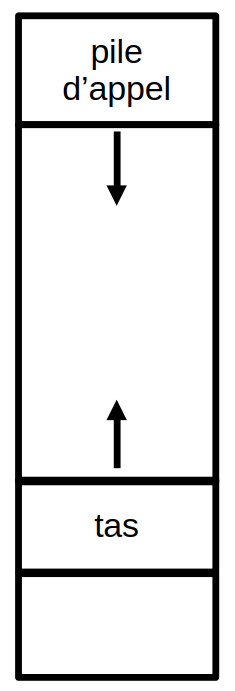
\includegraphics[height=6cm]{lecon/23-archi-assembleur/pile.png}
\end{minipage} \qquad
\begin{minipage}{0.6\linewidth}
	\begin{principe}    
		Le tas gère les données accessibles depuis tout le programme (malloc).
		
		Dans la pile, on met les variables locales à une fonction. A chaque nouvel appel, on empile de l'espace pour l'appel de fonction, que l'on enlève quand on return.
	\end{principe}
\end{minipage}

\paragraph{Développement :} Explication de la pile d'appel et implémentation en assembleur

\chapter{Echange de données et routage. Exemples.} \label{L24}
\textit{Y a une version sur les pads, mais bon, elle laisse peut-être un peu à désirer}

\chapter{Client-serveur : des sockets TCP aux requêtes HTTP} \label{L25}
\debut{Emile Martinez}{Lycée}{Aucun}{Tannenbaum, Balabonski 1ère}

\section{Modèle Client-Serveur}

\subsection{Le modèle}

\begin{definition}[Client/Serveur]
	Dans un réseau informatique, les échanges de données entre deux ordinateurs sont souvent asymétriques. Un ordinateur, désigné comme le client, demande généralement des ressources (des données) à un autre ordinateur, appelé serveur, qui les fournit à tous ceux qui en font la demande.
\end{definition}

\begin{example}
	En tapant «http://www.google.fr», votre machine va chercher à entrer en communication avec le serveur portant le nom «google.fr». Votre machine est ici client.
\end{example}

\begin{rem}
	N'importe quel type d'ordinateur peut jouer le rôle de serveur, mais dans le monde professionnel les serveurs sont des machines spécialisées conçues pour fonctionner 24h sur 24h.
\end{rem}

\begin{personalise}[Schéma] \\
	\label{25-modele}
	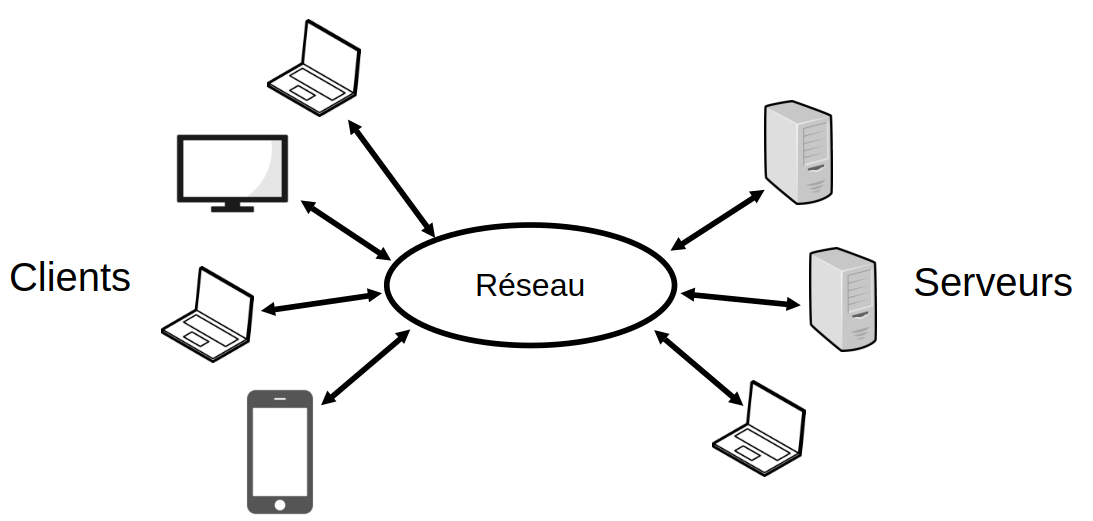
\includegraphics[width=0.7\linewidth]{lecon/25-client-serveur/modele.png}
\end{personalise}

\begin{rem}
	Un même ordinateur peut être à la fois plusieurs clients et plusieurs serveur 
\end{rem}

\begin{rem}
	Dans ce modèle les clients ne communiquent pas entre eux (ni les serveurs entre eux). Seuls des clients communiquent avec des serveurs
\end{rem}

\subsection{Caractéristiques concrètes}

\begin{principe}
	Caractéristiques d'un serveur : \begin{itemize}[label=$\star$]
		\item Son adresse IP est permanente, et le serveur attend une connexion entrante sur un ou plusieurs ports. On dit qu'il écoute.
		\item A la connexion d'un client sur le port en écoute, il ouvre une socket (interface de connexion)\footnote{traduction proposée par wikipédia, mais qui ne semble pas universellement admise}. Il n'est pas à l'initiative de la connexion
		\item A la suite de la connexion, le processus serveur communique avec le client suivant un protocole établi préalablement. L'action réalisée par le serveur en réponse à la requête client est souvent appelée service.
	\end{itemize}
\end{principe}

\begin{principe}
	Caractéristiques d'un client : \begin{itemize}
		\item Il est à l'initiative de l'établissement la connexion avec le serveur
		\item Lorsque la connexion est acceptée par le serveur, il communique comme le prévoit la couche application du modèle OSI
	\end{itemize}
\end{principe}

\begin{com}
	Bon ces deux caractérisations demandent à être améliorées, et éventuellement élaguées. De plus, on peut se poser la question si pour bien expliquer que ce n'est pas en tant que tel une machine qui est client ou serveur, mais une application/un programme, on pourrait pas mettre «caractéristiques d'un programme serveur /client». Mais un client pouvant être plus qu'un programme \dots. Tout cela demande réflexion.
\end{com}

Le protocole d'échange se divise alors ici en deux couches : la couche transport et la couche application.

\begin{definition}[Couche transport]
	 C'est le trait de la machine vers le réseau dans le schéma \ref{25-modele}. C'est le protocole qui met sur le réseau les données et qui les en récupèrent. (ex : TCP, UDP)
\end{definition}

\begin{definition}[Couche application]
	C'est la manière de choisir quelle données on veut échanger et de quelle manière on les envoie. Par analogie, choisir un protocole applicatif, c'est comme choisir une langue dans laquelle communiquer.
\end{definition}

\subsection{Est-ce tout internet ?}

Vous avez peut-êre entendu parler de protocole pair-à-pair, sans serveurs, et où les données s'échangent entre clients

\begin{personalise}[Schéma]\\
	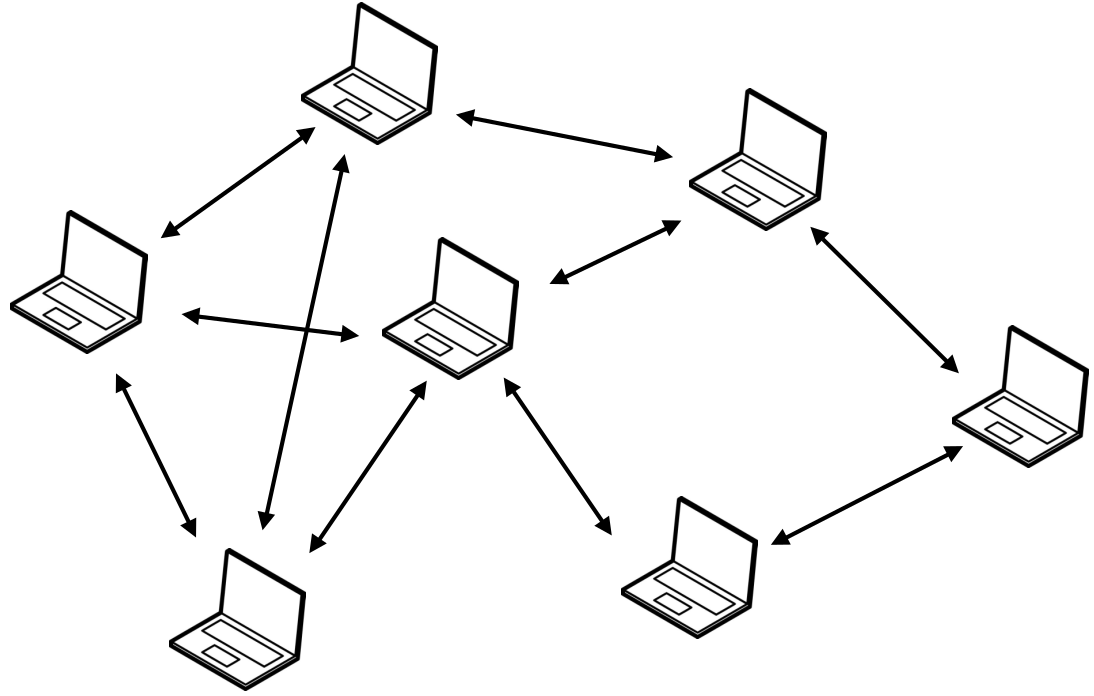
\includegraphics[width=0.5\linewidth]{lecon/25-client-serveur/pair-a-pair.png}
\end{personalise}

En réalité, nous sommes encore dans le modèle client serveur. En effet, chaque client joue alternativement le rôle de client et de serveur.

\begin{rem}
	L'ancien modèle de communication téléphonique fonctionnait en connectant directement les deux hôtes via un canal qui leur était réservé.
\end{rem}

\section{La couche transport}

\subsection{Introduction}

\begin{definition}[numéro de port]
	Les protocoles de transport définissent un numéro de port, c'est à dire un identifiant numérique associé à une application particulière. Il permet à une même machine d'établir plusieurs communication réseau en parallèle.
\end{definition}

\begin{example}
	Le numéro de port par défaut pour le web non sûr (protocole HTTP) est le 80, et celui pour le web sécurisé (HTTPS) est le 443. Ce ne sont cependant que des conventions, un serveur web peut attendre des connexions sur un autre port.
\end{example}

\begin{principe}[Principe de Segmentation]
	Plutôt que d'envoyer toutes les données d'un seul tenant, la couche transport les découpe en plein de paquets plus petits qu'on envoie séparemment.\end{principe}
\begin{personalise}[Intérêts] \begin{itemize}[label=$\star$]
		\item Plusieurs paquets peuvent cohabiter sur un même lien (plus équitables)
		\item En cas de paquet perdu ou corrompu, on peut ne renvoyer que le paquet en question (et pas tout le message)
		\item On peut exploiter la redondance des liens du réseau en faisant emprunter plusieurs chemin à différents paquets
	\end{itemize}
\end{personalise}

\begin{principe}[Principe d'encapsulation]
	Chaque couche du réseau ajoute un en-tête aux données que l'on envoie, et considère les données d'un bloc (sans différencier les données d'éventuels en-tête de couches précédentes).\begin{center}
		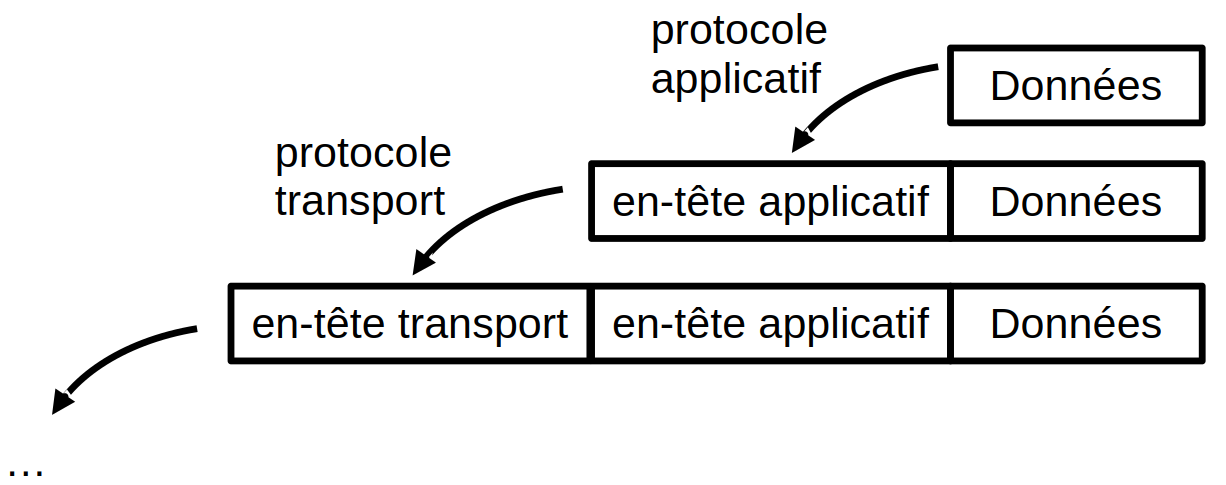
\includegraphics[width=0.6\linewidth]{lecon/25-client-serveur/encapsulation.png}
	\end{center}
\end{principe}

\subsection{Le protocole TCP}

\begin{principe}
	\label{25-tcp}
	Le protocole TCP permet, après l'initialisation d'une connexion, d'envoyer des données de taille arbitraire, dans l'ordre, de détecter les erreurs de transmission et de retransmettre les fragments de données perdus ou corrompus.
\end{principe}

\paragraph{Étape 1 :} Connexion en 3 temps\\
\begin{minipage}{0.4\linewidth}
	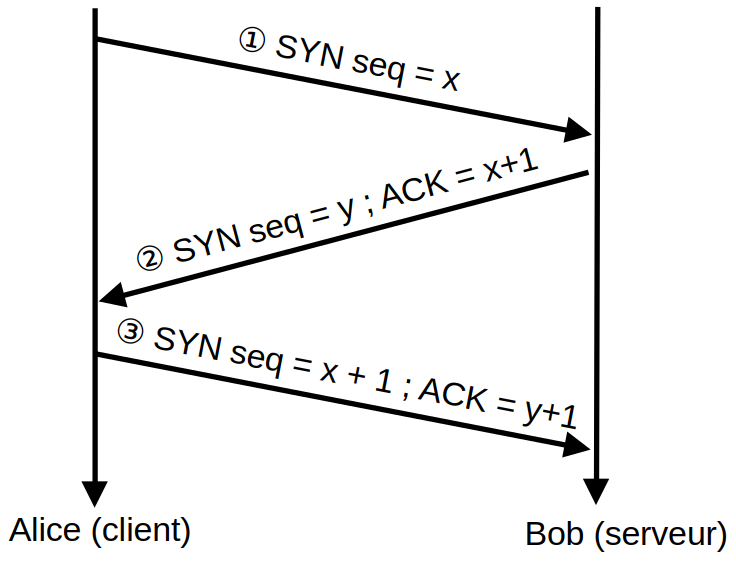
\includegraphics[width=\linewidth]{lecon/25-client-serveur/3-temps.png}
\end{minipage} \quad\begin{minipage}{0.55\linewidth}
	\begin{itemize}
		\item[$\circled{1}$] Le client choisit un numéro de séquence aléatoire et envoie un paquet SYN (pour synchronisation) indiquant ce numéro
		\item[$\circled{2}$] Le serveur reçoit le paquet et choisit un autre numéro aléatoire et renvoie un paquet SYN - ACK (synchronized - acknowledgment) contenant le numéro de séquence du client incrémenté de 1 et son propre numéro de séquence.
		\item[$\circled{3}$] Le client reçoit le paquet. Il est considéré comme connecté ! Il envoie «bien reçu» grâce au paquet ACK y+1
	\end{itemize}
	A la reception de ce paquet, le serveur est connecté
\end{minipage}

\paragraph{Étape 2 :} Transfert de données et retransmission\\
\begin{minipage}{0.4\linewidth}
	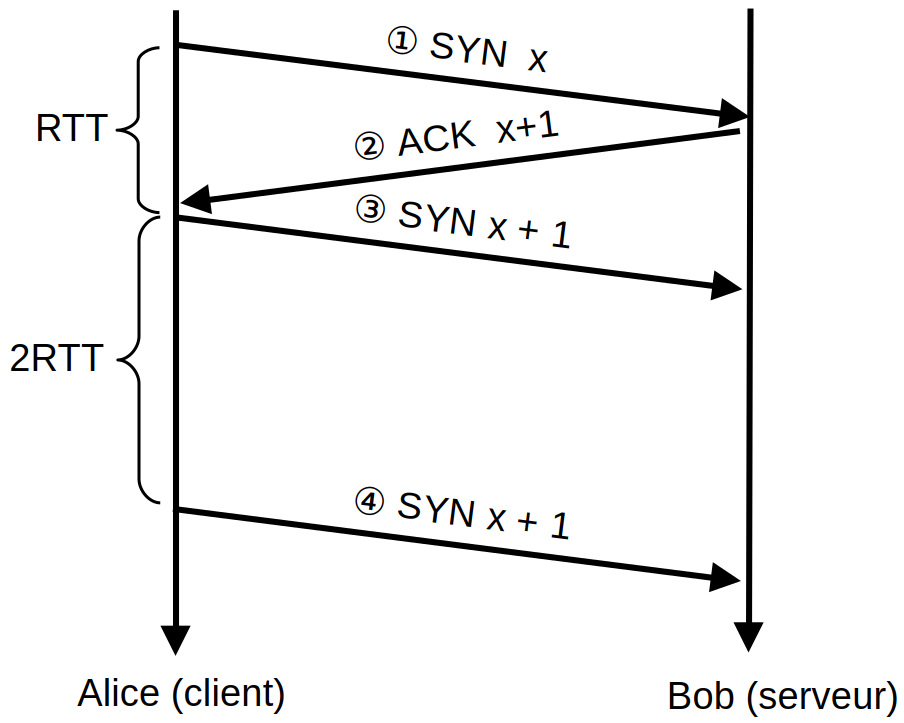
\includegraphics[width=\linewidth]{lecon/25-client-serveur/transfert-tcp.png}
\end{minipage} \quad \begin{minipage}{0.55\linewidth}
	\begin{itemize}
		\item[$\circled{1}$] Alice envoie un paquet de données identifié par un numéro de séquence.
		\item[$\circled{2}$] Bob le reçoit et indique la bonne réception avec un paquet ACK
		\item[$\circled{3}$] Alice n'a toujours pas reçu le ACK après 2 RTT = 2 fois le temps moyen d'un aller retour. Elle renvoie le paquet.
	\end{itemize}
\end{minipage}

\begin{rem}
	Les numéros de séquences nous permettent d'envoyer le paquet suivants avant d'avoir reçu l'acquittement du précédent, tout en restant fiable (cf. principe \ref{25-tcp}) (car on sait alors les remettre dans l'ordre, et à quel paquet correspond un acquittement).
\end{rem}

\paragraph{Développement :} La fenêtre glissante dans le protocole TCP pour augmenter le taux d'envoi et éviter la congestion.

\subsection{Socket TCP en Python}

\begin{definition}
	Une socket est une interface logicielle, c'est à dire un objet qui représente le bout de la connexion entre deux machines.
\end{definition}

\begin{algo}
	\begin{lstlisting}[style=PythonStyle]
# serveur TCP python
from socket import socket 
serveur = socket() #creation de la socket
serveur.bind(('0.0.0.0', 9999)) #port 9999
serveur.listen()
while True :
    #sclient : socket du client, adclient : addresse IP du client
    (sclient, adclient) = serveur.accept()
    # On attend que le client lui envoie au moins 1000 octets de données
    donnees = sclient.recv(1000)
    while donnees : 
        #traitement
        donnees = sclient.recv(1000)
    sclient.close()
	\end{lstlisting}
	\begin{lstlisting}[style=PythonStyle]
# client TCP python
from socket import socket
serveur = socket()
serveur.connect('127.0.0.1', 9999) #IP et port du serveur auquel se connecter
phrase = input()
while phrase != 'FIN':
	phrase = phrase + '\n'
	serveur.send(phrase.encode())
	phrase = input()
	\end{lstlisting}
\end{algo}

\section{La couche application}

Quand un client souhaite accéder à une page web, il tape un URL (ex : http://wikipedia.fr/informatique) dans la barre du navigateur web. Cette URL se découpe en 3 morceaux : \begin{itemize}
	\item http ou https qui précise le protocole de la couche application utilisé
	\item le nom de domaine (ex : wikipedia.fr) ou l'adresse IP du serveur
	\item le document demandé au serveur (ex : la page informatique du serveur wikipedia) 
\end{itemize}

\subsection{Le protocole HTTP (Hypertext transfer protocol)}

\begin{definition}
	Le protocole HTTP est un protocole applicatif qui définit les messages envoyés entre le navigateur (client) et le serveur. Les messages envoyés par le client sont des requêtes, ceux envoyés par le serveur des réponses. 
\end{definition}

\begin{definition}[méthode]
	Les requêtes d'un client commence par un mot clef qui indique la méthode utilisée, c'est à dire la nature du message envoyé. Les méthodes les plus communes sont GET, HEAD et POST.
\end{definition}

\begin{itemize}[label=$\star$]
	\item GET : Demande une ressource sans la modifier. C'est la méthode la plus courante pour demander d'afficher une page web par exemple
	\item POST : transmet une donnée (ex: envoi de forumlaire)
	\item HEAD : Cette méthode ne demande que des informations sur la ressource, sans demander la ressource elle-même
\end{itemize}

\begin{example}[navigation vers l'URL http://wikipedia.fr/informatique]
	Le client envoie la requête
	\begin{lstlisting}
GET /informatique HTTP/1.1
Host : www.wikipedia.fr
	\end{lstlisting}
	qui anonnce au serveur (wikipedia) que l'on utilise HTTP en version 1.1 pour obtenir la ressource informatique de wikipedia.\\
	
	Le serveur répond alors
	\begin{lstlisting}
HTTP/1.1 200 OK #accepte de communiquer et de transmettre la ressource
Serveur: wikipedia.fr
Date: 27.07.1214
Content-Type: text/html

<html class ="client...
<@et le reste de la page wikipedia visible à \url{view-source:https://fr.wikipedia.org/wiki/Informatique}@>
	\end{lstlisting}
	Si jamais la ressource demandée n'existe pas ou est indisponible, la réponse sera
	\begin{lstlisting}
HTTP/1.1 404 Not Found #ressource non trouvée
Server: wikipedia.fr
Date: 27.07.1214
Content-type:
<@suivi de la page html décrivant l'erreur@>
	\end{lstlisting}
\end{example}

\subsection{HTTPS}

Le protocole HTTP est clair : si une personne intercepte les paquets de données sur le réseau entre un client et un serveur, elle peut lire le contenu des messages échangés, par exemple des mots de passe confidentiels. Le protocole HTTPS fonctionne comme le protocole HTTP, mais en chiffrant les messages. 

\paragraph{Développement :} Le S du protocole HTTPS : authentification et chiffrement des messages.



\chapter{Architecture d'internet} \label{L26}
\debut{Emile Martinez}{}{Représentation binaire, graphes}{Tanenbaum, Balabonski 1ère, 2nd SNT Beaude Quenet}

\begin{com}
	On peut ici avoir une discussion sur le terme architecture. L'architecture c'est «Principe d'organisation d'un ensemble, agencement, structure». On peut donc penser à l'architecture physique. On parlerait alors des types de lien, de serveurs, de ou les placés, de qui controle quoi, de la mainère de faire des routeurs, etc. Néanmoins plus proches des notions du programme, on parlera plus ici d'architecture logicielle. Donc l'architecture conceptuelle, les différents protocoles qui s'empilent pour faire fonctionné cela. 
\end{com}

\section{Mise en Contexte}

\subsection{Historique}

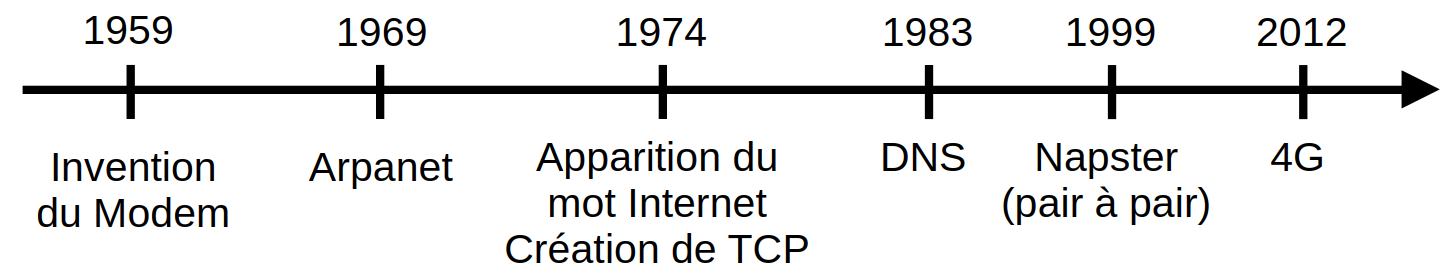
\includegraphics[width=\linewidth]{lecon/26-architecture-internet/frise.png}

\subsection{Maintenant}

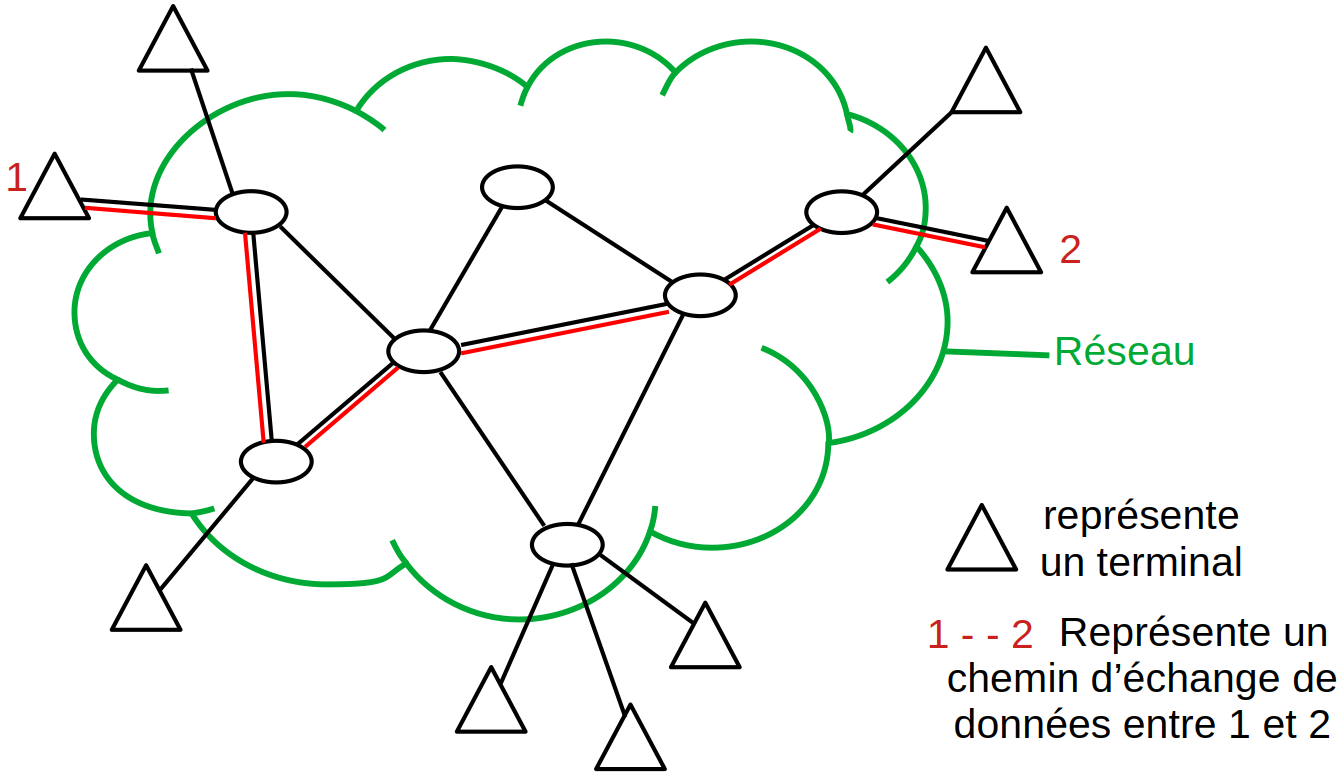
\includegraphics[width=\linewidth]{lecon/26-architecture-internet/chemin_reseau.png}

Désormais, des milliards d'utilisateurs sont connectés à travers l'internet.

\section{Modèles des couches OSI}

Fais le lien entre les besoins d'une application et les messages transitant sur internet

\begin{tabular}{p{0.45\linewidth}:p{0.45\linewidth}}
	\begin{center}
		\textbf{\textcolor{blue}{\underline{Réseau}}}
	\end{center} &
	\begin{center}
	\textbf{\textcolor{blue}{\underline{Poste}}}
	\end{center} \\
	&\\
	
	\begin{minipage}{\linewidth}
		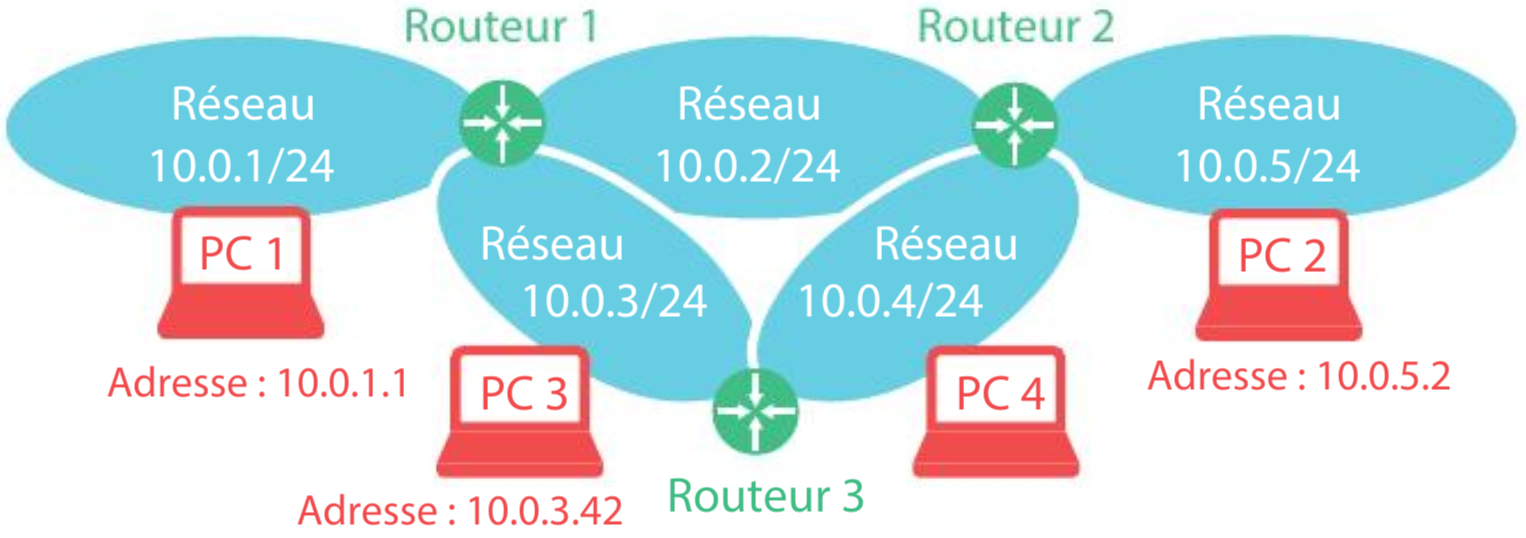
\includegraphics[width=\linewidth]{lecon/26-architecture-internet/schema_osi.png} \\ \\
		(schém honteusement volé de ce livre https://www.mesmanuels.fr/acces-libre/9782278094912)
	\end{minipage} & \raisebox{-0.5\height}{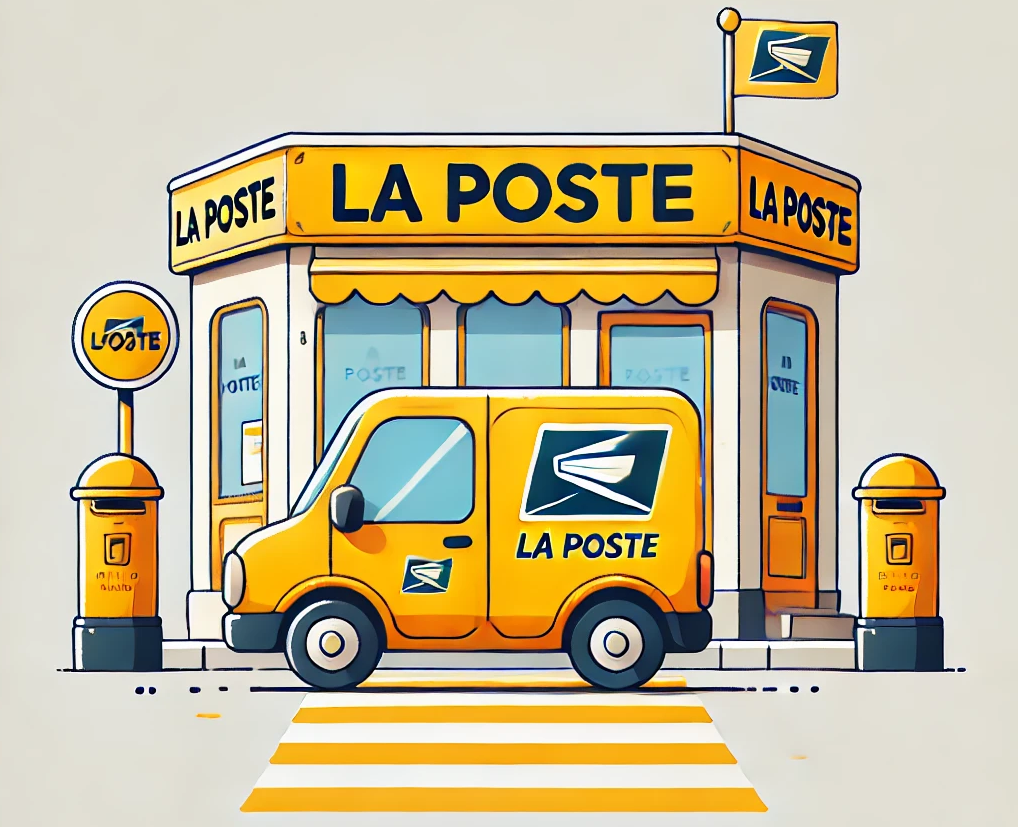
\includegraphics[width=\linewidth]{lecon/26-architecture-internet/poste.png}} \\
	& \\ \hdashline
	
	\multicolumn{2}{c}{\underline{Couche Applicative}} \\
	Fais le lien entre les besoins d'une application et les messages transitant sur internet &
	Manière de lire et écrire une lettre. Langue dans laquelle on comunique \\
	&\\ \hdashline
	
	\multicolumn{2}{c}{\underline{Couche Transport}} \\
	Centralise les données qu'envoient différentes applications d'une même machine et les mets sur le réseau. C'est le lien entre le PC et le réseau & poster le courrier, aller le chercher dans la boite aux lettres, et le repartir entre les différentes habitants \\
	&\\ \hdashline
	
	
	\multicolumn{2}{c}{\underline{Couche Réseau}} \\
	S'occupe de faire passer les données d'un réseau à un autre. C'est là qu'on décide la direction que doit prendre la donnée. C'est ce qu'on appelle le routage. & Centre de tri (ou bureau de poste) mettant en sac postal et donnant le prochain lieu ou doit aller le sac postal \\
	&\\ \hdashline
	
	
	\multicolumn{2}{c}{\underline{Couche Lien}} \\
	Achemine les données à l'intérieur d'un réseau & le kangoo jaune, le train entre deux gare de triage, le porteur qui amène le sac de lettre du quai au wagon postal, etc\dots
\end{tabular}

\begin{rem}
	La structure d'internet est assez indépendante de la technologie sous-jacente. Comme l'organisation de la poste ne dépend que à la marge du véhicule qu'utilise le facteur.
\end{rem}

\begin{personalise}[Conséquence]
	La technologie peut évoluer en conservant le travail des couches supérieures (et même plus généralement entre les couches)
\end{personalise}

\begin{com}
	On parle plus de l’indépendance de la structure physique que des couches entre elles car le programme demande d'insister dessus.
\end{com}

\subsection{Paquets}

\begin{principe}[Principe de segmentation]
	Plutôt que d'envoyer toutes les données d'un seul tenant, on les découpe en plein de paquets plus petits qu'on envoie séparément.
\end{principe}

\begin{personalise}[Intérêts]
	\begin{itemize}
		\item Plusieurs paquets peuvent cohabiter sur un même lien (il est facile de dire qu'on envoie un paquet de chaque application à tour de rôle par exemple)
		
		\item Si un paquet est corrompu ( des données à l'intérieur sont fausses) ou se perd, on est pas obligé de tout renvoyer, on peut ne renvoyer que le morceau abîmée
		
		\item On peut maximiser la redondance des liens du réseau en faisant emprunter plusieurs chemin à différents paquets
	\end{itemize}
\end{personalise}

\begin{principe}[Principe d'encapsulation]
	Chaque protocole ajoute un en-tête à chaque paquet pour échanger de l'information, et considère l'en-tête d'avant comme de la données.\\
	\\
	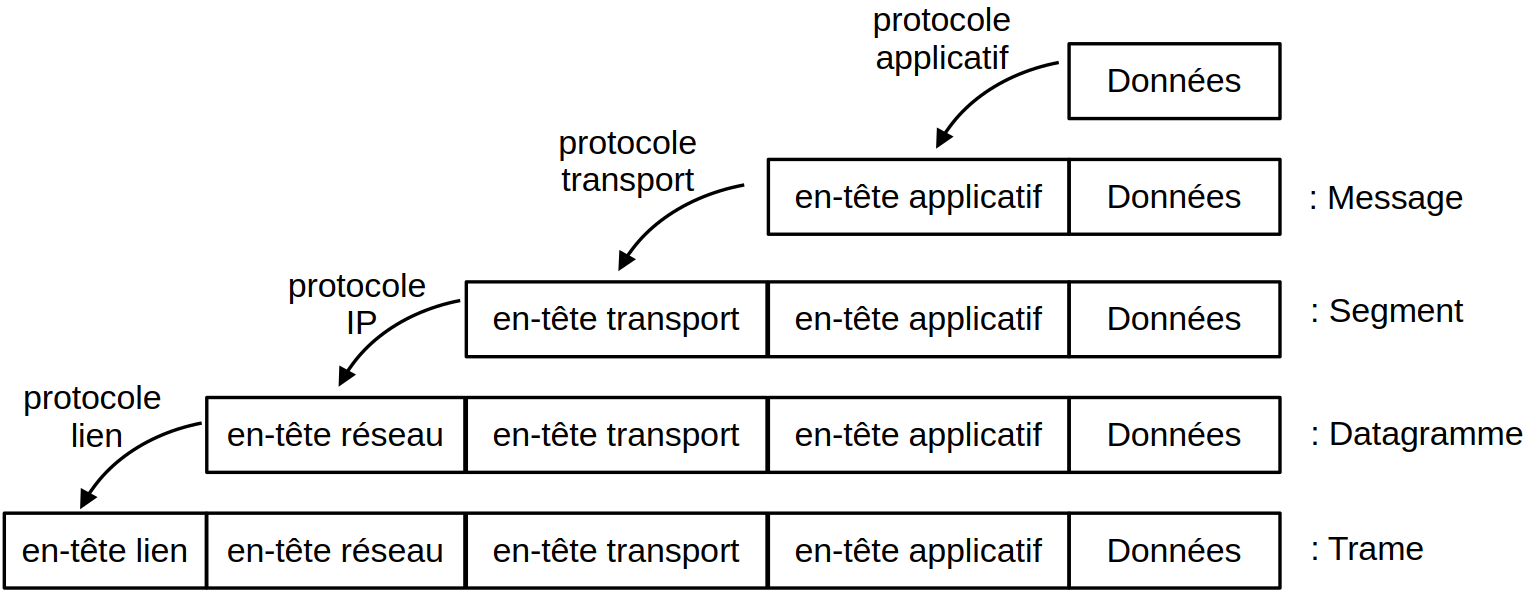
\includegraphics[width=\linewidth]{lecon/26-architecture-internet/encapsulation.png}
\end{principe}

\begin{com}
	Ce schéma pourrait être l'occasion de question avec les élèves, en expliquant plus longuement le principe, puis en leur demandant à leur avis à quelle couche le message est le plus grand (est ce que l'applicatif vient par dessus le transport ou l'inverse). Néanmoins il y a peu de chances qu'ils trouvent. On peut donc éventuellement plutôt le faire, et ensuite poser cette question en devoir.
\end{com}

\subsection{Principe d'un protocole}

\begin{definition}[protocole]
	Un protocole est une manière de faire sur laquelle les différentes parties se mettent d'accord en amont.
\end{definition}

Pour chaque couche et pour chaque chose que l'on veut faire dans cette couche, en réseau, on a des protocoles.

\begin{example}
	Dans l'analgoie de la poste, la manière d'écrire une adresse sur une enveloppe est un protocole  (que l'on pourrait placer à la couche réseau)
\end{example}

\begin{example}
	\begin{itemize}
		\item NTP est un protocole applicatif permettant de syncrhoniser les horologes des ordinateurs
		
		\item FTP est un protocole applicatif permettant d'échanger des fichiers (comme des courriels)
		
		\item UDP est un protocole de la couche transport sans garantie utilisé pour transmettre des flux vidéos
		
		\item DHCP est un protocole de la couche réseau permettant à un nouvel utilisateur d'obtenir une adresse IP
		
		\item Ethernet est un protocole de la couche liaison décrivant comment se transmettre des paquets dans un câble coaxial
	\end{itemize}
\end{example}

\section{Des protocoles structurants}

\subsection{Le protocole IPv4}

C'est un protocole de la couche réseau ayant pour but d'identifier les différents hôtes d'un réseau. Chaque hôte est identifié par un nombre de 32 bits, découpé en  4 nombres de 8 bits :
$$\texttt{1100000010101000000101000101101} \to \texttt{ 11000000.10101000.00010100.00101101} \to \texttt{192.164.10.45}$$

\noindent Paquet IP : \raisebox{-0.5\height}{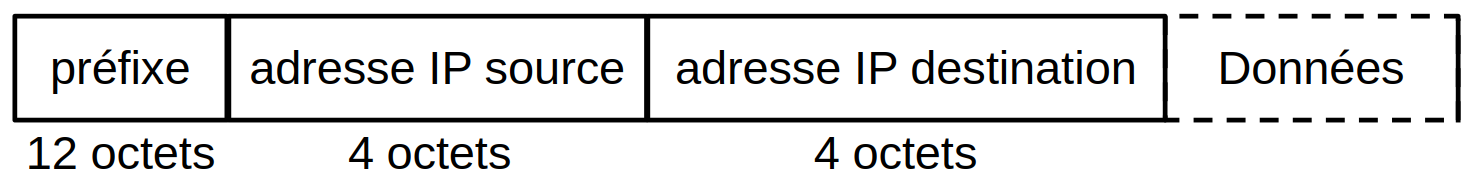
\includegraphics[width=0.7\linewidth]{lecon/26-architecture-internet/paquet_IP.png}}\\

Les routeurs (interfaces entre différents réseaux) garde alors une table de routage dans laquelle à chaque adresse IP est indiqué l'adresse IP du prochain routeur où aller.

\paragraph{Dveloppement :} Convergence de l'algorithme de Bellman-Ford

\begin{personalise}[Problème]
	Les tables sont beaucoup trop grandes
\end{personalise}

\begin{personalise}[Solution]
	Deux machines proches recevront des IPs proches et ainsi on regroupe des machines en sous-réseau, dont les premiers bits des IPs sont les mêmes. Le nombre de bits identiques d'un sous-réseau est indiqué par un nombre après le /x (appelés masque de sous-réseau). Une table de routage n'a alors plus qu'a sauvegarder les sous-réseaux (sauf si il est dans le sous-réseau, où il garderait alors plus)
\end{personalise}

\begin{example}
	\texttt{11000000.11000000.00001010.00101101/20} représente toutes les IP commençant par \texttt{11000000.11000000.0000}
\end{example}

\begin{principe}
	Il arrive que l'on attribue des adresses d'un sous réseau ailleurs. On utilisera alors le principe de correspondance du plus grand préfixe (on va dans le sous réseau valide, où le plus de bits correspondent)
\end{principe}

\begin{rem}
	Dans le champ préfixe on a des informations comme la version du protocole, un code de vérification (pour vérifier que le paquet n'est pas corrompu) ou encore le TTL (time to leave) indiquant le nombre de sauts restants autorisés pour ce paquets (lui évitant de boucler à l'infini).
\end{rem}

\subsection{Le protocole TCP}

Le protocole TCP est un protocole de la couche transport, décidant donc de qui va être envoyé, ré-envoyé, et quand.

\begin{com}
	Si on veut s'étendre sur TCP, on peut reprendre ce qui est fait dans la leçon \ref{L25}, et même éventuellement en récupérer le développement. Néanmoins ça parait moins structurant pour l'architecture globale d'internet.
\end{com}

\begin{principe}
	\begin{itemize}
		\item Offrir des garanties sur les paquets : Pour cela il établit une connexion entre les deux hôtes (par une connexion en trois temps) puis envoie des acquittements pour chaque paquet (pouvant ainsi renvoyer ceux qui ne sont pas arrivés)
		
		\item Réguler le trafic : Pour cela, en fonction de la quantité de paquets perdus ou arrivant en retard, le protocole TCP adapte le taux d'envoi.
	\end{itemize}
\end{principe}

\begin{com}
	On pourrait également dans le premier point rajouter le fait que on peut réordonner les paquets
\end{com}

\subsection{Le protocole DNS}

C'est un protocole de la couche application, parfois appelé «l'annuaire d'internet», qui fait correspondre des adresses IP à des URL lisibles par l'homme. Pour cela, des serveurs répondent l'adresse IP demandée.\\

\begin{minipage}{0.5\linewidth}
	\begin{center}
		\begin{tikzpicture}[-]
			\node[rectangle, draw] (r) {Racine};
			\node[rectangle, draw, below left = 0.5cm and 1cm of r] (fr) {.fr};
			\node[rectangle, draw, below = 0.5cm of r] (com) {.com};
			\node[rectangle, draw, below right = 0.5cm and 1cm of r] (org) {.org};
			\node[rectangle, draw, below = 0.5cm of fr] (wiki) {wikipedia.fr};
			\node[rectangle, draw, below left = 0.5cm and -0.2cm of org] (agreg) {agreg-info.org};
			\node[rectangle, draw, below right = 0.5cm and -0.2cm of org] (w) {wikipedia.org};
			
			\draw (r) edge[] (fr);
			\draw (r) edge[] (com);
			\draw (r) edge[] (org);
			\draw (fr) edge[] (wiki);
			\draw (org) edge[] (agreg);
			\draw (org) edge[] (w);
			
		\end{tikzpicture}
	\end{center}
\end{minipage} \begin{minipage}{0.3\linewidth}
	Pour transformer un URL en adresse IP, on demande alors à chaque serveur l'adresse du serveur suivant.
\end{minipage}\\\\

\begin{personalise}[Schéma][Résolution d'une requête DNS] 
	\begin{center}
		\begin{tikzpicture}
			\node[rectangle, draw, inner sep=0.2cm] (dom) {www.domaine.org};
			\node [rectangle, draw, inner sep=0.2cm, above right = 1cm and 3cm of dom] (r) {Serveur Racine};
			\node [rectangle, draw, inner sep=0.2cm, right = 3cm of dom] (org) {Serveur .org};
			\node [rectangle, draw, inner sep=0.2cm, below right = 1cm and 3cm of dom] (sdom) {Serveur domaine.org};
			
			\draw ([yshift = 0.5cm]dom.east) edge[->, above left] node{1} ([yshift = 0.1cm]r.west);
			\draw ([yshift = 0.3cm]dom.east) edge[<-, below left] node{2} ([yshift = -0.1cm]r.west);
			\draw ([yshift = 0.1cm]dom.east) edge[->, above right] node{3} ([yshift = 0.1cm]org.west);
			\draw ([yshift = -0.1cm]dom.east) edge[<-, below right] node{4} ([yshift = -0.1cm]org.west);
			\draw ([yshift = -0.3cm]dom.east) edge[->, above left] node{5} ([yshift = 0.1cm]sdom.west);
			\draw ([yshift = -0.5cm]dom.east) edge[<-, below left] node{6} ([yshift = -0.1cm]sdom.west);
			
		\end{tikzpicture}
	\end{center}
\end{personalise}

\subsection{HTTP}

C'est un protocole omniprésent de la couche application. Il sert à échanger des pages web.\\

Son en-tête contient des informations comme le type de pages échangés, l'adresse correspondates, la date, etc. Il contient également un champ méthode précisant quel type d'opération l'on veut faire :
\begin{itemize}
	\item GET pour obtenir une page WEB
	\item POST pour envoyer des données au serveur
	\item PUT qui modifie ce que contient le serveur
	\item pas de méthode coté serveur mais un code de réussite :\begin{itemize}
		\item[200] réussite de la réqueté
		\item[404] la page n'existe pas
	\end{itemize}
\end{itemize}

\begin{com}
	En vrai on montrerait une requête HTTP pour que l'on comprenne là c'est peu clair. On verrait alors en toute lettre les informations, puis le script HTML de la page WEB qui se déploie.
\end{com}

\paragraph{Développement :} Le S de HTTPS

\chapter{Modèle relationnel et conception de bases de données} \label{L27}
\debut{Emile Martinez}{MPI}{}{}

Dans cette leçon, on illustrera les concepts avec une situation concrètes minimales : un grossiste a une liste de produits dont des clients font la commande.

\begin{personalise}[Objectif]
	Stocker des données de façon à les rendre facilement utilisables, modifiables, etc.
\end{personalise}

\begin{personalise}[Solution naïve]
	Convertir une commande en chaîne de caractères et les stocker dans un grand fichier.
\end{personalise}

\begin{example}
	{ produit : tomate, prix : 3 quantité : 50, client : Le navet naviguant, adresse : 13 rue du Swag à Tarbes },  { produit : patate, prix : 1, quantité : 30, client : Le navet naviguant, adresse : 13 rue du Swag à Tarbes },
\end{example}

\begin{personalise}[Problème]
	Beaucoup de redondances, recherche compliqué
\end{personalise}

\section{Schéma Entité-Association}

\begin{idee}
	Pour éviter les redondances, on stocke à part les clients, les produite. Ensuite on stocke les les liens entre les deux.
\end{idee}

On se place alors dans un paradigme appelé relationnel.

\begin{definition}
	Un schéma entité association est un graphe non orienté composé :
	\begin{itemize}[label=$\star$]
		\item de sommet appelés entités
		\item d'arêtes appelés relations
		\item d'étiquettes sur les arêtes : A une arête $(u,v)$, on associe un étiquette $(x,y)$ ($(v,u)$ sera étiqueté par $(y,x)$) avec $x$ et $y$ pouvant prendre les valeurs : 0..1, 0..*, 1..1 1..*
		\item des attributs sur les sommets et les arêtes précisant ce qu'ils représentent.
	\end{itemize}
\end{definition}

\begin{idee}
	\begin{itemize}
		\item les entités représentent les types des objets (par exemple les clients, les villes, les produits, etc.)
		\item les arêtes représentent les liens (par exemple le fait que un client habite dans telle ville)
		\item les étiquettes sur les arêtes indiquent combien un objet précis peut avoir de liens, la première valeur étant le minimum, la deuxième le maximum ( * représentant donc $+\infty$ )
		\item les attributs représentent les composantes (ex : le nom du client)
	\end{itemize}
\end{idee}

\begin{personalise}[Représentation]
	Les entités sont des carrés, les relations des traits avec un losange au milieu, les étiquettes sont aux bases des arêtes, et les attributs des bulles liés à leur objet.
\end{personalise}

\begin{example}\\
	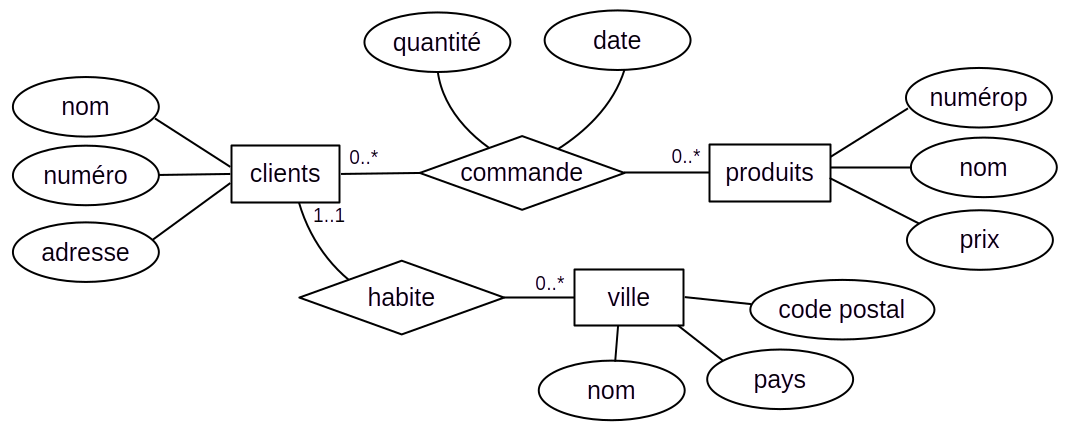
\includegraphics[width=\linewidth]{lecon/27-relationnel-bd/exemple_relationnel.png}
\end{example}

\begin{rem}
	Si on veut que chaque client ait au moins une commande, on met 1..* sur son étiquette associée à commande.
\end{rem}

\begin{proposition}
	On peut convertir les relations ..* ..* en entité
\end{proposition}

\begin{example}\\
	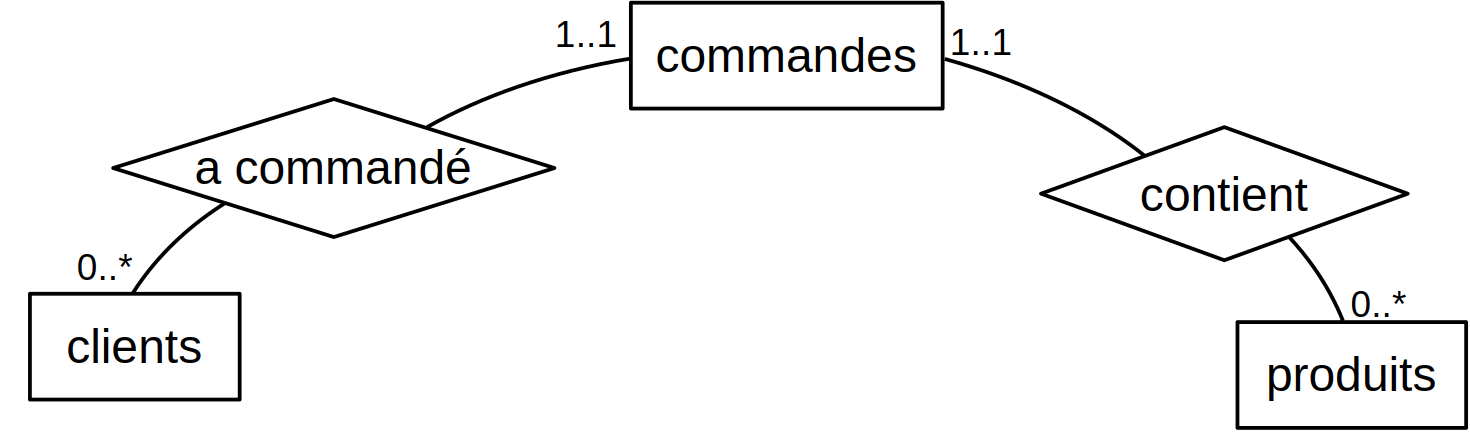
\includegraphics[width=0.8\linewidth]{lecon/27-relationnel-bd/changement_reltionnel.png}
\end{example}

\section{Modèle relationnel}

\subsection{Définitions}

On cherche maintenant une manière de modéliser ce schéma pour le stocker en machine.

\begin{definition}
	\begin{itemize}[label=$\star$]
		\item Un domaine est un ensemble, fini ou non, de valeurs possibles ayant un nom (ex : $(\N, \text{"poids"})$, $(\text{flottant}, \text{"taille"})$, $(\{true, false\}, \text{"present"})$, $(\text{les chaines de caractères}, \text{"nom"})$, etc.)
	
		\item Si $(D1, nom_1), \dots, (D_n, nom_n)$ sont des domaines, on appelle schéma de table (ou schéma de relation) le produit cartésien $D_1 \times D2 \dots \times D_n$ où chaque $D_i$ représente une colonne (ou attributs) représenté par le nom $nom_i$
	
		\item Une table (ou relations) est un sous ensemble du produit cartésien d'un schéma de table.
	
		\item Un enregistrements (ou entrée, ligne, n-uplet) est un élément (donc un n-uplet) d'une table.
	\end{itemize}
\end{definition}

\begin{idee}
	Néanmoins, quand on a un ensemble de tables, on veut qu'elle puisse respecter des règles.
\end{idee}

\begin{example}
	On peut vouloir que les clients mentionnés dans une commande existent en vrai.
\end{example}

\begin{definition}
	\begin{itemize}[label=$\star$]
		\item Une clé d'une table est un ensemble de colonnes tel qu'il n'existe pas deux enregistrements ayant les mêmes valeurs sur ces colonnes.
		
		\item Une clé minimale est une clé qui perd sa propriété si on enlève un attribut
		
		\item Chaque table doit avoir une clé primaire (qui est une clé minimale que l'on choisit)
		
		\item Une clé étrangère est un ensemble de colonne d'une table $t_1$, correspondant à un ensemble de colonnes de $t_2$, et tel que dans tout enregistrement de $t_1$, les $p$-uplets des valeurs des colonnes de la clé étrangère existe dans les colonnes correspondantes de $t_2$.
		
		\item Une contrainte de domaine, imposant à chaque enregistrements d'une table de vérifié une assertion logique.
	\end{itemize}
\end{definition}

\begin{personalise}[Représentation]
	On écrit sous la forme n$om_{table}(attributs1, attributs2, \dots)$ en soulignant les attributs issu d'une clé primaire et en mettant un \# devant les clés étrangères.
\end{personalise}

\begin{example}\\
	\texttt{client(\underline{numero}, nom, \#(code\_postal, pays), adresse)}\\
	\texttt{ville(\underline{code\_postal, pays}, nom)}\\
	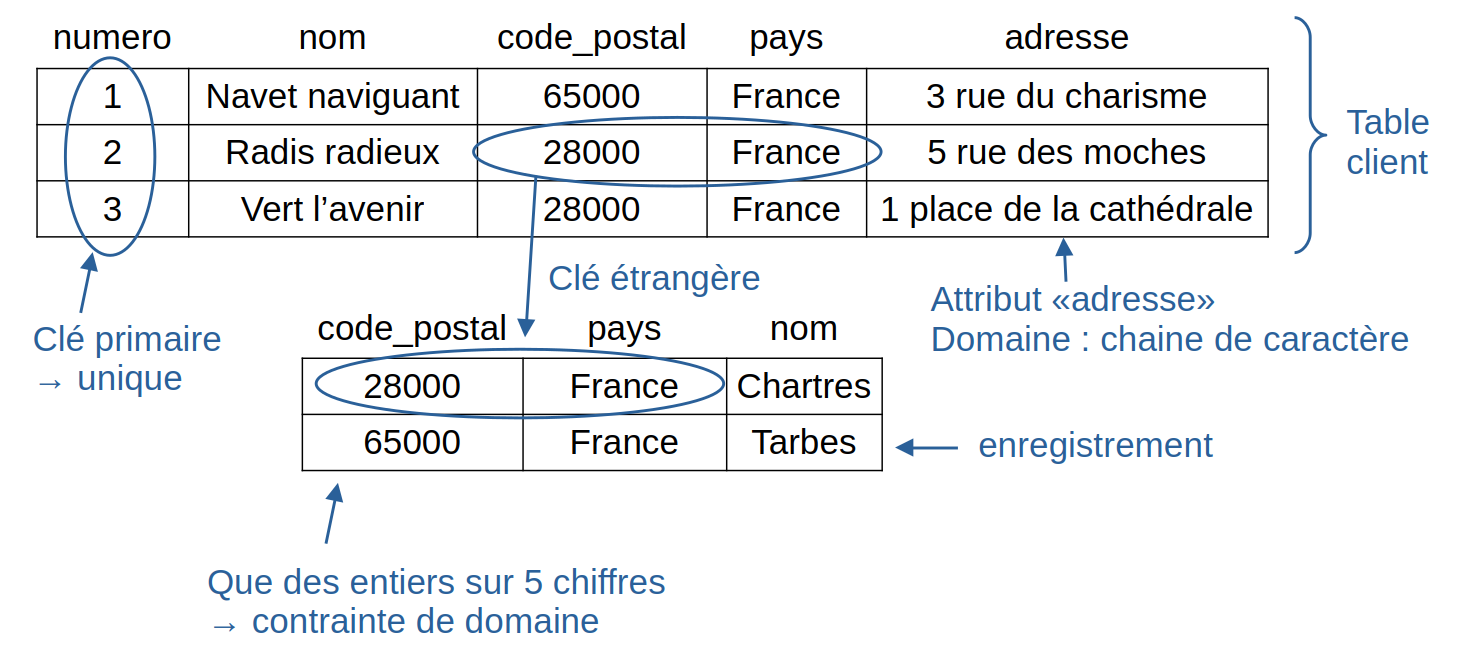
\includegraphics[width=\linewidth]{lecon/27-relationnel-bd/exemple_table.png}
\end{example}

\subsection{De l'entité association au modèle relationnel}

\begin{algo}
	\begin{itemize}[label=$\star$]
		\item Les entités deviennent des relations
		
		\item Pour les associations 1..1 0..* on crée une contrainte de clé étrangère dans la première base vers la clé primaire de la deuxième
		
		\item Pour les associations 0..*  0..* on crée une troisième entité contenant les clés primaires des deux tables, chacune étant des clés étrangères
		
		\item Pour les associations 1..*   1..* on fait la même chose mais les clés étrangères sont dans les tables initiales
		
	\end{itemize}
	
	etc.
\end{algo}

\begin{example}\\
	\texttt{Produit(\underline{numérop}, nom, prix, poids)}\\
	\texttt{Clients(\underline{numéro}, nom, adresse, \#(code\_postal, pays))}\\
	\texttt{Commande(\underline{\#num\_produit, \#num\_client}, quantite)}\\
	\texttt{Ville(\underline{code\_postal, pays}, nom)}
\end{example}

\paragraph{Développement :} Modélisation par une base de données relationnelle d'élèves inscrit à l'université

\section{Implémentation}

\subsection{SGBD}

\begin{definition}
	Un SGBD (système de gestion de bases de données) est un système implémentant les bases de données, permettant d'effectuer des opérations dessus (création, insertion, modification, sélection de certains types de données, etc.) tout en masquant la complexité des opérations.
\end{definition}

\begin{example}
	Exemple de SGBD relationnel : PostgreSQL, MySQL, duckDB, Oracle
\end{example}

\begin{rem}
	Il existe aussi des SGBD ne fonctionnant pas en relationnel. (exemple : IMS)
\end{rem}

\begin{definition}
	 Une transaction est un ensemble d'instruction qui doivent toutes être exécutées ou toutes annulées.
\end{definition}

\begin{example}
	On veut supprimer des produits et donc toutes les commandes attenantes. Si on commence par supprimer par le produit, puis qu'on s'interrompt au milieu de la suppression des commandes,  on aura une base incohérente.
\end{example}

\begin{proposition}
	 Un bon SGBD, doit avoir la propriété ACID pour :
	
	\paragraph{Atomicité :} Une transaction est un tout. Soit tout est fait, soit rien
	
	\paragraph{Cohérence :} Les transactions doivent faire passer la base d'un état cohérent à un autre état cohérent. Les contraintes du modèle relationnel doivent être respectées (clé, clé étrangère, domaine, etc.)
	
	\paragraph{Isolation :} Si deux transactions s'exécutent simultanément, alors leur execution doit produire le même effet que si elle avait était effectué séquentiellement (en particulier, on ne doit pourvoir observer l'état intermédiaire d'une autre transaction)
	
	\paragraph{Durabilité :} Une transaction validé l'est définitivement : un problème (une panne de courant, un cable qui se casse, etc...) ne doit pas mettre à mal la pérennité de la mise à jour.
\end{proposition}

\subsection{SQL}

Pour communiquer avec un SGBD relationnel, a était défini un langage de programmation : le SQL (structured query language).

\begin{rem}
	Ce langage ne dépendant pas de l'implémentation sous-jacente, on ne donne que le résultat que l'on veut et pas la manière de l'obtenir. C'est donc un langage dit déclaratif, dans le paradigme logique.
\end{rem}

\begin{rem}
	Grâce à SQL, les bases de données sont très expressives et donnent de multiples possibilités (théorème de CODD)
\end{rem}

\begin{exercise}
	Trouver le plus de manière possible de chercher le max et faire la division. \label{27-exo-dev2}
\end{exercise}

\paragraph{Développement 2 :} Correction de l'exercice \ref{27-exo-dev2}

\begin{com}
	Ici mettre le développement sur les bases du langages SQL serait plus adaptés à la leçon (en tant qu'introduction à SQL) mais le but étant également de montrer que l'on sait faire des choses, ce développement là est plus intéressant.
\end{com}


\chapter{Requêtes en langage SQL} \label{L28}
\debut{Emile Martinez}{Terminale (II) / MPI (III)}{Schéma entité association / Modèle relationnel}{}

Pendant toute la leçon on se base sur l'exemple suivant :

\begin{center}
	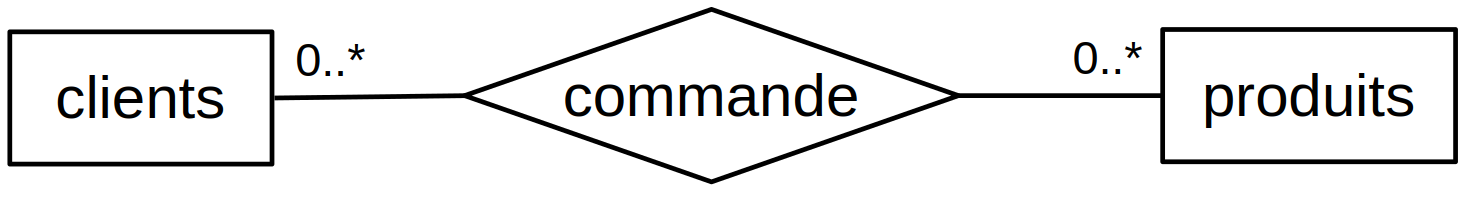
\includegraphics[width=0.6\linewidth]{lecon/28-sql/schema-EA.png}
\end{center}

\noindent \texttt{Produits(\underline{num\_produit}, nom, prix, poids)}\\
\texttt{Clients(\underline{num\_client}, nom, adresse, ville)}\\
\texttt{Commande(\underline{\#num\_produit, \#num\_client}, quantite)}

\section{Les tables}

\begin{definition}
	Une table est un tableau où chaque colonne est étiqueté par un attribut et contient des données du même type, et où chaque ligne est appelé un n-uplet, une entrée ou encore un enregistrement.	
\end{definition}

\begin{example}
	Table produits :
	\begin{center}
		\begin{tabular}{|c|c|c|c|}
			\hline num\_produit & nom & prix & poids \\ \hline
			1 & pomme & 1,5 & 1 \\ \hline
			2 & poulet & 7 & 2 \\ \hline
			3 & patate & 2 & 1 \\ \hline
		\end{tabular}
		\\
		\enspace \\
		\underline{produits}
	\end{center}
\end{example}

\section{Requêtes de bases (Terminale)}

\subsection{Requêtes de sélection}

Une requête de selection prend en entrée une ou plusieurs tables et les transforme en une nouvelle table.

\begin{syntaxe}
	\texttt{FROM} : appelle une table\\
	\texttt{SELECT} : selectionne les colonnes (projection)
\end{syntaxe}

\begin{example}
	Affichage du nom de tous les produits
	\begin{lstlisting}
SELECT nom
FROM produits
	\end{lstlisting}
\end{example}

\begin{syntaxe}
	\texttt{WHERE} est utilisé avant une sélection pour filtrer les n-uplets. Il est suivi d'une condition booléenne : seules les entrées la satisfaisant seront renvoyées
\end{syntaxe}

\begin{example}
	Affichage du nom des produits coutant moins que 50€
	\begin{lstlisting}
SELECT nom
FROM produits
WHERE prix < 50
	\end{lstlisting}
\end{example}

\begin{rem}
	Dans un \texttt{WHERE}, on a le droit aux opérations entières, à $<$, $>$, $=$, \texttt{AND}, \texttt{OR}, \texttt{NOT}
\end{rem}

\begin{syntaxe}
	\texttt{table1 \texttt{JOIN} table 2 \texttt{ON} condition} crée la table des éléments de table1 et de table2 (avec les colonnes des deux tables) en ne gardant que les lignes qui vérifient la condition.
	
	On peut alors renommer une table avec un alias après \texttt{AS} pour différencier les attributs de mêmes noms.
\end{syntaxe}

\begin{example}
	Les noms des produits présents dans une commande de gros (avec plus de 10 éléments)
	\begin{lstlisting}
SELECT p.nom
FROM produit AS p JOIN
     commande AS c ON p.num_produit = c.num_produit
WHERE c.quantite > 10
	\end{lstlisting}
\end{example}

\begin{syntaxe} Autres mot clefs :
	\begin{itemize}[label=]
		\item \texttt{DISTINCT} (après \texttt{SELECT}) pour ne garder que les lignes différentes
		
		\item \texttt{SELECT *} pour afficher toutes les colonnes
		
		\item \texttt{ORDER BY attributs ASC} (resp. \texttt{DESC}) (à la fin de la requête) qui trie les éléments par ordre croissant (resp. décroissant) selon attributs
		
		\item \texttt{LIMIT x OFFSET y} (à la fin de la requête) qui enlève les y premiers éléments et affiche seulement les x premiers restants
	\end{itemize}
\end{syntaxe}

\subsection{Invention et mise à jour}

\begin{syntaxe}[Requête d'insertion]
	On ajoute un n-uplet dans une table avec le mot-clef \texttt{INSERT INTO} suivi du nom de la table et du n-uplet.
\end{syntaxe}

\begin{example}
	\begin{lstlisting}
INSERT INTO produit VALUES (1, "baguette", 1.20, 200), 
                           (2, "pates", 1.5, 500)
;
	\end{lstlisting}
\end{example}

\begin{syntaxe}[Requête de suppression]
	 On utilise \texttt{UPDATE} et \texttt{SET} pour modifier les données d'une table, suivi d'un \texttt{WHERE} qui selectionne les lignes à modifier
\end{syntaxe}

\begin{example}
	\begin{lstlisting}
UPDATE produit SET prix = 1.3 WHERE id = 1;
	\end{lstlisting}
\end{example}

\begin{syntaxe}[Requête de supression]
	\texttt{DELETE FROM table WHERE condition} supprime de la table tous les n-uplets vérifiant cond
\end{syntaxe}

\begin{example}
	\begin{lstlisting}
DELETE FROM produit
WHERE id = 2
	\end{lstlisting}
\end{example}

\begin{proposition}
	Si une requête de modification viole une contrainte (clef primaire déjà présente, suppression d'un élément dont la clé est étrangère dans une autre table, etc.) la requête n'est pas effectuée
\end{proposition}

\paragraph{Développement : Premiers pas en SQL}

\section{Pour aller plus loin (Prépa)}

\subsection{Types de données en SQL}

SQL possède de nombreux types de données. Les types peuvent être numériques (\texttt{INT}, \texttt{DECIMAL}, \texttt{REAL}), textuels (\texttt{CHAR(n)}, \texttt{VARCHAR(n)}, \texttt{TEXT}) ou plus spécifiques comme \texttt{DATE} et \texttt{TIME}.\\

Sur ces types s'appliquent les opérations de comparaisons : \texttt{<=}, \texttt{<}, \texttt{=}, \texttt{<>} (= $\neq$),  \texttt{>}, \texttt{>=}

\begin{rem}
	Les types \texttt{DATE} et \texttt{TIME} sont des chaines de caractères. La comparaison se fait donc d'après l'ordre lexicographique. Néanmoins, leur format et tel que la comparaison est la même que selon la date représenté
\end{rem}

\begin{rem}
	Sur les types numériques il y a aussi les opérations mathématiques usuelles.
\end{rem}

\begin{definition}
	La valeur \texttt{NULL} représente l'absence de valeur
\end{definition}

\begin{proposition}
	Toute comparaison avec la valeur \texttt{NULL} donnera au final quelque chose de faux
\end{proposition}

\begin{example}
	\begin{lstlisting}
SELECT *
FROM produit
WHERE NOT(NULL = NULL) OR NOT(NULL <> NULL)
	\end{lstlisting}
renverra une table vide.
\end{example}

\begin{syntaxe}
	Pour tester si un attribut est à \texttt{NULL}, on utilise \texttt{IS NULL} et \texttt{IS NOT NULL}
\end{syntaxe}

\subsection{Requêtes ensemblistes}

Les opérateurs ensemblistes permettent de combiner dans un résultat unique des lignes provenant de deux (ou plus) requêtes. Les lignes peuvent venir de tables différentes mais après projection on doit obtenir des tables ayant même schéma de relation (même attributs).\\

Les opérateurs ensemblistes sont les suivants : 
\begin{itemize}[label=$\bullet$]
	\item \texttt{UNION} : pour obtenir l'union des deux requêtes

	\item \texttt{INTERSECT} : pour obtenir l'intersection des deux requêtes

	\item \texttt{EXCEPT} : pour obtenir la différence entre deux requêtes
\end{itemize}

\begin{example}
    Noms de tous les protagonistes de la base
	\begin{lstlisting}
SELECT nom FROM produit
UNION
SELECT nom FROM clients
	\end{lstlisting}
\end{example}

\begin{syntaxe}
	On peut également faire un produit cartésien de tables. On peut le faire avec un \texttt{JOIN . ON 1=1} mais on peut également simplement mettre une virgule entre tables \texttt{,} ce qui fera un produit cartésien.
\end{syntaxe}

\begin{exercise}
	Faire une jointure uniquement à l'aide de produit cartésien et de la clause \texttt{WHERE}
\end{exercise}

A mi-chemin entre le produit et la jointure il y a les jointures externes.

\begin{syntaxe}[Jointures externes]
	Dans une jointure externe, l'une des tables utilisées est directrice : tous ses renseignements seront présents dans la table résultante même s'ils n'ont pas de valeurs correspondantes avec les autres tables de la requête. Les colonnes de l'autre table seront alors remplies de \texttt{NULL}.
	\begin{itemize}
		\item \texttt{LEFT JOIN} : retourne tous les n-uplets de la table gauche même si la condition n'est pas vérifiée dans l'autre table
		\item \texttt{RIGHT JOIN} : retourne tous les n-uplets de la table droite même si la condition n'est pas vérifiée dans l'autre table
		\item \texttt{FULL JOIN} : union du left join et du right join
	\end{itemize}
\end{syntaxe}

\begin{com}
	Si on a la place ici on peut également mettre un exemple, e.g. (j'ai rien trouvé de super donc j'ai pas mis d'exemple, mais si on voulait afficher toutes les commandes mais que l'on voulait que tous les clients apparaissent)
\end{com}

\begin{syntaxe}
	On peut utiliser dans une clause de condition le mot clé \texttt{attributs IN requete} qui permet de savoir si attributs est présent dans le résultat de requête.
\end{syntaxe}

\begin{rem}
	On appelle cela une requête imbriquée.
\end{rem}

\begin{example}
	\begin{lstlisting}
SELECT VILLE
FROM CLIENTS
WHERE num_client IN (SELECT num_client FROM commandes)
	\end{lstlisting}
\end{example}

\subsection{Requêtes agrégatives}

\begin{definition}
	Un agrégat est un partitionnement horizontal d’une table en sous-table en fonction des valeurs d’un ou plusieurs attributs de partitionnement.
\end{definition}

\begin{personalise}[Schéma]
	\begin{tabular}{|c|c|}
		\hline 1 & pomme \\
		\hline 2 & poulet \\
		\hline 1 & navet \\
		\hline 2 & pomme \\
		\hline
	\end{tabular} $\qquad \to \qquad$ \begin{tabular}{|c|c|}
		\hline \multirow{2}{*}{1} & pomme \\
		\cline{2-2} & navet \\
		\hline \multirow{2}{*}{2} & poulet \\
		\cline{2-2} & pomme \\
		\hline 
\end{tabular}
\end{personalise}

\begin{syntaxe}
	\texttt{GROUP BY attribut} crée cette agrégation.
\end{syntaxe}

On peut alors appliquer des fonctions statistiques qui seront appliquées à chaque agrégat : \begin{itemize}[label=$\bullet$]
	\item \texttt{COUNT(*)} : compte le nombre de valeur de la sous-table
	\item \texttt{SUM(attribut)} : somme les valeurs de attribut sur la sous table
	\item \texttt{AVG(attribut)} : calcule la valeur moyenne
	\item \texttt{MAX} (resp. \texttt{MIN}) \texttt{(attribut)} : calcule la valeur maximum (resp. minimum)
\end{itemize}

\begin{syntaxe}
	Pour filtrer les sous-tables que l'on veut garder en utilisant après le \texttt{GROUP BY} par une clause \texttt{HAVING condition}, où la condition peut contenir des requêtes agrégatives.
\end{syntaxe}

\begin{example}
	Listes des villes ayant au moins 5 clients
	\begin{lstlisting}
SELECT ville
FROM clients
GROUP BY ville
HAVING COUNT(*) >= 5
	\end{lstlisting}
\end{example}

\paragraph{Développement 2 :} Requêtes avancées, avec ou sans agrégation

\chapter{Langages rationnels et automates finis. Exemples et applications.}\label{L29}
\debut{Emile Martinez}{MPI}{définition inductive, définition de base sur les langages}{}

\begin{com}
	On considère les définitions de bases sur les langages (mot vide, concaténation de deux mots, etc.) parce que on a déjà beaucoup de choses à dire, et que on peut le considérer antérieur à la leçon.
\end{com}

\begin{com}
	Dans le dilemne classique de présenter d'abord les langages régulier ou d'abord les autoamtes, on choisit ici les langages, car la notion de langages est nécessaire pour parler de langage reconnu par un automate. Donc pour ne pas faire d'aller retour sur les notions de langages, on définit d'abord les langages réguliers.
\end{com}

\section{Langages réguliers}

\subsection{Langages}

\begin{definition}
	Un langage sur un alphabet $\Sigma$ est une ensemble de mot de $\Sigma$
\end{definition}

\begin{example}
	Pour $\Sigma = \{0,1\}, \emptyset, \{\varepsilon, 101, 1111\}, \{\varepsilon\}, \{\text{mot de taille paires}\}$ sont des langages sur $\Sigma$
\end{example}

\begin{definition}
	On proloonge les définitions ensemblistes d'union, intersection et complémentaire sur les langages.On définit aussi : \begin{itemize}[label=$\star$]
		\item la concaténation de $L_1$ et $L_2$ par $\{u.v / u \in L_1, v \in L_2\}$ noté $L_1.L_2$
		\item inductivement $L^n$ par $L^0 = \{\varepsilon\}$ et $L^n = L^n-1 . L$
		\item l'étoile de Kleene par $L^* = \bigcup\limits_{n \geq 0} L^n$
	\end{itemize}
\end{definition}

\subsection{Langages réguliers}

\begin{definition}
	On définit par induction l'ensemble des expressions régulières sur $\Sigma$ par : \begin{itemize}[label=$\star$]
		\item les cas de bases : $\empty$, $\varepsilon$, $a \in \Sigma$
		\item le constructeur unaire ${}^*$
		\item les constructeurs binaires $+$ et $.$ (en notation infixe)
	\end{itemize}
\end{definition}

\begin{example}
	$(0+1)^*.1.0$ est une expression régulière
\end{example}

\begin{definition}
	Le langage $L(r)$ associé à une expression régulière est définit inductivement par : \begin{itemize}[label=$\bullet$]
		\item $L(\emptyset) = \emptyset$, $L(\varepsilon) = \{\varepsilon\}$, $L(a) = \{a\}$ pour $a \in \Sigma$
		\item $L(r_1 + r_2) = L(r_1) \cup L(r_2)$
		\item $L(r_1.r_2) = L(r_1).L(r_2)$
		\item $L(r^*) = L(r)^*$
	\end{itemize}
	On appelle $L(r)$ un langage régulier.
\end{definition}

\begin{example}
	$L\big((0+1)^*.1.0\big)$ est l'ensemble mots représentant des nombres en binaires multiples de 2 et pas de 4.
\end{example}

\section{Automates}

\subsection{Automates non déterministes}

\begin{com}
	On commence par les automates non déterministes et pas les déterministes, non pas car ils sont plus simples (la défintion peut l'être car on a pas la fonction partielle à gérer). Néanmoins, en s'autorisant les $\varepsilon$-transition, la définition d'un mot reconnu est plus complexe. On fait cela car la définition de DFA se dérive mieux de celle de NFA que l'inverse, et faire pleinement les deux définitions feraient beaucoup de répétitions. Ce qui peut etre appréciable ou pas suivant le niveau de la classe. (Pas dans un plan d'agreg avec une classe qui suit moyennenment, on pourrait faire dans l'autre sens, de manière à profiter de la répétition pour les familiariser avec le formalisme et les définitions).
	
	De plus beaucoup de définitions en sont aussi légèrement simplifiés par la suite (automates complet, équivalence DFA, NFA). Meme si ce dernier argument est pas tip top.
\end{com}

\begin{definition}
	Un automate fini non déterministe (NFA) est un 5-uplet $(Q, \Sigma, q_0, F, \delta)$ où : \begin{itemize}
		\item $Q$ est un ensemble fini d'états
		\item $\Sigma$ est un alphabet
		\item $q_0 \in Q$ l'état initial
		\item $F \subset Q$ l'ensemble des états acceptants (ou finaux)
		\item $\delta : Q × \{\Sigma \cup \varepsilon\} \to \mathcal P(Q)$ une fonction de transition
	\end{itemize}
\end{definition}

\begin{rem}
	$\delta(q, \varepsilon)$ est une $\varepsilon$-transition
\end{rem}

\begin{personalise}[Représentation]
	Les états sont des cercles, les transitions des flèches étiquetées. Une flèche entrante dans l'état initial, sortante pour $q\in F$
\end{personalise}

\begin{example}
	\label{29-eg}
	\raisebox{-0.7\height}{
	\begin{tikzpicture}[->]
		\node (r1) {};
		\node[state, right=of r1] (q0) {0};
		\node[state, right=of q0] (q1) {1};
		\node[state, right=of q1] (q2) {2};
		\node[right=of q2] (r2) {};
		
		\draw (r1) edge[] (q0);
		\draw (q0) edge[loop below] node{0, 1} (q0);
		\draw (q0) edge[below] node{0} (q1);
		\draw (q1) edge[below] node{1} (q2);
		\draw (q2) edge[] (r2);
	\end{tikzpicture}}
\end{example}

\begin{exercise}
	Sur l'exemple précédent, définir formellement l'automate $(Q, \Sigma, q_0, F, \delta)$
\end{exercise}

\begin{definition}
	Soit $\mathcal A = (Q, \Sigma, q_0, F, \delta)$ un NFA. On appelle $\varepsilon$-fermture de l'état $q$, noté $E(q)$ l'ensemble $\bigcup\limits_{n \geq 0} \delta^n_\varepsilon(\{q\})$ où \raisebox{-0.5\height}{$\begin{array}{rccl} 
		\delta_\varepsilon : & \mathcal P(Q) & \to & \mathcal P(Q)\\
		& A & \mapsto & \bigcup\limits_{q \in A} \delta(q, \varepsilon)
	\end{array}$}
\end{definition}

\begin{idee}
	$E(q)$ est l'ensemble des états accessibles depuis $q$ en empruntant seulement des $\varepsilon$-transition.
\end{idee}
\begin{definition}
	On définit $\delta^*$ sur $Q\times \Sigma$ par induction sur les mots par :\begin{itemize}[label=$\star$]
		\item $\delta^*(q, \varepsilon) = E(q)$
		\item $\delta^*(q, wa) = E\left(\bigcup\limits_{q' \in \delta^*(q, w)} \delta^*(q', a)\right)$
	\end{itemize}
\end{definition}

\begin{example}
	Sur l'exemple \ref{29-eg}, $\delta^*(0, 10) = \{0, 2\}$
\end{example}

\begin{definition}
	On dit que $w \in \Sigma^*$ est accepté par un NFA $\mathcal A$ si $F \cap \delta^*(q_0, w) \neq \emptyset$. On note $\mathcal L(\mathcal A)$ le langage des mots reconnu par $\mathcal A$. On dit que le langage $\mathcal L(\mathcal A)$ est reconnaissable.
\end{definition}

\begin{example}
	Pour l'exemple \ref{29-eg}, $\mathcal L(\mathcal A) = \{w \in \{0, 1\}^* / w \text{ termine par } 01\}$
\end{example}

\begin{definition}
	On dit que deux automates sont équivalents si ils reconnaissent le même langage.
\end{definition}

\subsection{Automates déterministes}

\begin{definition}
	Soit $\mathcal A$ un NFA. Si $\forall q \in Q, \forall a \in \Sigma, |\delta(q, a)| \leq 1$ et $\delta(q, \varepsilon)=\emptyset$, on dit que $\mathcal A$ est un automate fini déterministe (DFA)
\end{definition}

\begin{proposition}
	Si $\mathcal A$ est un DFA, alors $\forall q \in Q, \forall w \in \Sigma^*, |\delta^*(q, w)| \leq 1$.
\end{proposition}

\begin{exercise}
	Reprendre la définition d'un DFA (et d'un langage reconnu) avec des fonctions partielles dans $Q$ à la place de fonctions dans $\mathcal P(Q)$.
\end{exercise}

\begin{definition}
	Un langage rationnel est un langage reconnu par un automate déterministe.
\end{definition}

\begin{example} DFA reconnaissant les mots sur $\Sigma=\{0, 1\}$ de longueur impaire\\
	\begin{tikzpicture}[->]
		\node (r1) {};
		\node[state, right=of r1] (q0) {0};
		\node[state, right=of q0] (q1) {1};
		\node[right=of q1] (r2) {};
		
		\draw (r1) edge[] (q0);
		\draw (q0) edge[bend left, above] node{0, 1} (q1);
		\draw (q1) edge[bend left, below] node{0, 1} (q0);
		\draw (q1) edge[] (r2);
	\end{tikzpicture}
\end{example}

\begin{theorem}
	Tout NFA est équivalent à un DFA.
\end{theorem}

\begin{proof}
	Construction de l'automate des parties
\end{proof}

\begin{example}
	
	\begin{minipage}{0.5\linewidth}
		\begin{tikzpicture}[->]
			\node (r1) {};
			\node[state, right=of r1] (q0) {0};
			\node[state, right=of q0] (q1) {0, 1};
			\node[state, right=of q1] (q2) {0, 2};
			\node[right=of q2] (r2) {};
			
			\draw (r1) edge[] (q0);
			\draw (q0) edge[loop above] node{0} (q0);
			\draw (q0) edge[bend left, above] node{1} (q1);
			\draw (q1) edge[bend left, below] node{1} (q0);
			\draw (q1) edge[bend left, above] node{0} (q2);
			\draw (q2) edge[bend left, below] node{1} (q1);
			\draw (q2) edge[bend left=70, above] node{0} (q0);
			\draw (q2) edge[] (r2);
		\end{tikzpicture} 
	\end{minipage} \begin{minipage}{0.4\linewidth}
		est un DFA équivalent au NFA de l'exemple \ref{29-eg}
	\end{minipage}
	
\end{example}

\begin{rem}
	Dans le pire des cas, déterminiser un NFA crée un nombre exponentiel d'états
\end{rem}

\begin{definition}
	On dit que un DFA $\mathcal A$ est complet si $\forall q \in Q, \forall a \in \Sigma, |\delta(q, a)| = 1$
\end{definition}

\begin{theorem}
	Tout DFA est équivalent à un DFA complet.
\end{theorem}

\section{Lien automate fini et langages réguliers}

\begin{theorem}[Kleene]
	Pour $L \in \Sigma^*$, $L$ régulier $\Leftrightarrow$ $L$ rationnel.
\end{theorem}

\begin{proof}
	$\Leftarrow$ : Construction de Thompson
	
	$\Rightarrow$ : Algorithme d'élimination des parties (Brozowski)
\end{proof}

\paragraph{Développement :} Construction de Thompson

\begin{rem}
	L'algorithme de Thompson nous fournit un NFA avec beaucoup d'$\varepsilon$-transitions. On voudrait les éviter.
\end{rem}

\begin{definition}
	Soit $L \subset \Sigma^*$ un langage. On définit : \begin{itemize}
		\item $P(L) = \{a \in \Sigma | a.\Sigma^* \cap L \neq \emptyset\}$
		\item $D(L) = \{a \in \Sigma | \Sigma^*.a \cap L \neq \emptyset\}$
		\item $F(L) = \{(a,b) \in \Sigma \times \Sigma | \Sigma^*.ab.\Sigma* \cap L \neq \emptyset\}$
	\end{itemize}
	$L$ est local si $L\backslash \{\varepsilon\} = P(L)\Sigma^* \enspace \cap \enspace \Sigma^*D(L) \enspace \big\backslash \enspace \Sigma^*\left(\Sigma^2 \backslash F(L)\right) \Sigma^*$
\end{definition}

\begin{rem}
	L est local si il est déterminé par ses premières et dernières lettres et par ses facteurs de 2 lettres.
\end{rem}

\begin{definition}
	Soit $L \subset \Sigma^*$. On définit $Loc(L)$ l'automate $(Q_L, \Sigma, q_0, F_L, \delta_L)$ tel que : \begin{itemize}
		\item $Q_L = \{q_a / a \in \Sigma\} \cup \{q_0\}$
		\item $F_L = \{q_a / a \in D(L)\} \cup \{q_0 / \varepsilon \in L\}$
		\item $\delta_L : \left\{ \begin{array}{ll} 
			\delta(q_0, a) \mapsto q_a & \text{pour }a \in P(L)\\
		\delta(q_a, b) \mapsto q_b & \text{pour } ab \in F(L)
		\end{array} \right.$
	\end{itemize}
\end{definition}

\begin{com}
	Ici on a la défintion avec des fonctions partielles et non une fonction qui renvoie $\emptyset$ ou un singleton. On peut remplacer dans la définition, mais comme vu dans l'exercice juste après la définition, c'est la même chose.
\end{com}

\begin{theorem}
	Si $L$ est local, alors $L = \mathcal L(Loc(L))$
\end{theorem}

\begin{algo}[Berry Sethi]
	\textbf{Entrées :} $r$ une expression régulière\\
	\textbf{Sorties :} Un NFA sans $\varepsilon$-transition qui reconnait $\mathcal (r)$
	\begin{enumerate}
		\item Linéariser $r$ en $r'$ (en marquant chaque lettre pour la rendre unique)
		\item Construire $Loc_{\mathcal L(r')}$ (en calculant $P$, $D$, etc.)
		\item Sur les transitions de l'automate, effacer les marquages
	\end{enumerate}
\end{algo}

\subsection{Conséquences}

La première conséquence évidente est de vérifier l'appartenance à un langage régulier. Mais il y a d'autres conséquences plus théoriques.

\begin{theorem}
	Les langages réguliers sont clos par complémentaire et intersection
\end{theorem}

\begin{theorem}[Lemme de l'étoile]
	Soit $L \subset \Sigma^*$ régulier. Alors, $\exists n \in \N \: : \: \forall w \in L, \, |w| \geq n+1 \implies \exists x, y, z \: : \: w = x.y.z $ et \begin{enumerate}
		\item $|xy| \leq n$
		\item $|y|\geq 1$
		\item $\forall i \in \N x.y^i.z \in L$
	\end{enumerate} 
\end{theorem}

\begin{proof}
	On prend le $\mathcal A$ le DFA tel que $\mathcal L(\mathcal A) = L$, $n$ son nombre d'états.
\end{proof}

\begin{rem}
	Ce lemme est surtout utilisé pour prouver la non rationnalité d'un langage.
\end{rem}

\begin{example}
	Montrer que $\{a^n b^n \: / \: n \in N\}$ n'est pas rationnel.
\end{example}

\section{Applications}

\begin{com}
	Si on veut on peut rajouter ici une partie  sur un exemple concret, pour voir l'utilité des automates. Par exemple pour la solution à un passage de rivière (ou on doit faire traverser une rivière à un chou une chèvre et un loup, on doit faire des allers retours en ne pouvant à chaque fois en emporter qu'un ou 0 dans le bateau, sans laisser sans surveillance la chèvre et le chou ou la chèvre et le loup). On représente alors les états comme ou sont les animaux et le bateau, les lettres comme qui traverse, les états finaux comme ve que l'on souhaite (tout le monde a traversé), les états ou l'on perd sont des puits, et on veut savoir si le langage reconnu est vide, et si il ne l'est pas, ca nous donne toutes les solutions possibles.  (on peut alors généraliser avec pas seulement trois animaux, etc.)\\
	
	Néanmoins, bien qu'intéressant pour illustrer la puissance de modélisation des automates (comme le suggère un peu le programme), cet exemple semble le premier à devoir sauter vu sa pertinence moindre dans un cadre purement informatique (on fait moins de liens avec des problèmes informatiques concrets)
\end{com}

\subsection{Analyse lexicale}

Les expressions régulières et les DFA interviennent dans la compilation des langages de programmation, au niveau de l'analyse lexicale.

\begin{principe}
	Découper un programme en lexème, interprétables. Pour cela, on utilise un analyseur lexicale, qui est une liste d'automate que l'on exécute en parrallèle. Quand on bloque sur tous les automates, on prend l'automate dans l'état final de plus haute priorité.
\end{principe}

\begin{example} \\
	lexème 1 : $(O..9)^+ . ','.(0..9)^*$ (flottant)\\
	lexème 2 : $(0..9)^+$ (int) \\
	lexème 3 : $if$ (IF) \\
	lexème 4 : $then$ (THEN) \\
	lexème 5 : $\Sigma \backslash '\enspace'$ (variables).\\\\
	\texttt{if (1) then 42,5} est reconnu comme IF INT("5") THEN FLOAT(42,5)
\end{example}

\subsection{Expression régulière POSIX}

\begin{personalise}[Motivation]
	\texttt{grep 'reg\_exp' fichier} renvoie toutes les lignes de fichier ont une osus-chaîne est dans $\mathcal L(reg\_exp)$
\end{personalise}

\begin{syntaxe}
	\begin{itemize}[label=$\bullet$]
		\item un caractère représente lui-même en général
		\item | représente le $+$
		\item * représente l'étoile de Kleene
	\end{itemize}
	etc. (voir \texttt{man grep})
\end{syntaxe}

\subsection{Reconnaissance de motif dans un texte}

Mais les automates, ont aussi des applications en eux-mêmes.\\

On considère que $u$ est un sous mot de $w$ s'il existe $k \in \N$ tel que $u = w(k)...w(k+|u|-1)$

\begin{personalise}[Motivation]
	CTRL + F
\end{personalise}

\begin{personalise}[Solution naïve]
	$O(|t| \times |w|)$ (On parcourt $t$ et on compare les lettres une à une)
\end{personalise}

\begin{personalise}[Autre solution]
	On construit l'automate des motifs en $O(P(|w|))$ où $P$ est un polynôme, reconnaissant $\Sigma^*m\Sigma^*$, et on détecte ensuite si $w$ est un sous-mot de $t$ en $O(|t|)$.
\end{personalise}

\paragraph{Développement :} Construction de l'automate des motifs

\subsection{Automates en architectures des ordinateurs}

Une version modifiée des automates (sans états final, avec des sorties à chaque transition) est très utilisée en architecture des ordinateurs, servant à représenter comment doit agir un circuit électronique, et dont on peut parfois espérer déduire une manière de l'implémenter, ou a défaut, une manière de le spécifier.

\begin{com}
	Si on veut on peut s'étendre ici, en parlant de situation par lesquelles on peut implémenter un automate (par exemple le protocole MESI), ou de comment implémenter un automate par un circuit séquentiel (avec un registre qui stocke l'état, et la fonction de transition (et éventuellement une fonction de sortie))
\end{com}


\chapter{Grammaires hors-contexte. Applications `a l’analyse syntaxique.}

\chapter{Classes P et NP. Problèmes NP-complets. Exemples.} \label{L31}
\debut{Emile Martinez}{}{}{}

Les notions présentées ici le sont informellement. Les notions formelles existent mais des notions intuitives suffisent à cette leçon.

\section{Introduction}

\subsection{Problèmes de décision}

\begin{definition}
	Un problème de décision $\Pi$ est la donnée d'un ensemble $E$ d'instance et d'un ensemble $E^+\subset E$ d'instances positives.
\end{definition}

\begin{example}
	\begin{itemize}[label=$\bullet$]
		\item $E = \N$, $E^+ = \{n \in \N / n \text{ est premier}\}$
		\item $E = \{\text{formules du premier ordre}\}$, $E^+ =\{\text{formules universellement vraies}\}$
	\end{itemize}
\end{example}

\begin{personalise}[notation]
	Pour $\Pi$ un problème de décision $(E, E^+)$, on identife parfois $\Pi$ et $E^+$
\end{personalise}

\begin{example}
	$SAT = \Big( \{\text{formules propositionnelles}, \: \{\text{formules propositionnelles satisfiables}\}\}\Big)$. On peut alors noter $x\wedge y \in SAT$ mais $x\wedge \neg x\notin SAT$.
\end{example}

\begin{example}[Problème APP]\\
	\label{31-app}
	\textbf{Entrée} $T$ un tableau d'entiers, $x \in \N$\\
	\textbf{Sortie} $x \in T$
\end{example}

\begin{exercise}
	Réécrire le problème APP sous la forme $E,_, E^+$
\end{exercise}

\begin{rem}
	Quand on considère un problème en informatique, on ne considère pas des objets mathématiques mais un codage de ces objets. Dans la définition d'un problème, on rajoute parfois le codage de ces objets, sinon, on considère un codage «raisonnable».
\end{rem}

\begin{definition}
	La taille d'une instance d'un problème est la taille du codage de l'instance.
\end{definition}

\begin{example}
	Des tailles pour des structures de données classiques sont :
	\begin{itemize}	[label=$\star$]
		\item $O(\log(n))$ pour un entier $n$
		\item $O(|T| \times k)$ pour un tableau $T$ contenant des éléments de taille $k$
		\item $O(|A|\times \log(|S|))$ pour un graphe $G = (S, A)$
	\end{itemize}
\end{example}

\section{Algorithmes}

Ce qu'on appelle ici algorithme, c'est un programme C, avec une mémoire infini.

\begin{definition}
	On dit qu'un algorithme résout un problème $\Pi$ si sur chaque entrée possible, l'algorithme termine et renvoie la sortie correspondante.
\end{definition}

\begin{example}
	\label{31-pgcd}
	L'algorithme qui calcule le PGCD par soustraction successive et compare le résultat à $1$ résout le problème premier entre eux : $E = \N^2$, $E^+ = \{(a, b)\in \N^2 | a\wedge b = 1\}$
\end{example}

\begin{definition}
	On dit qu'un algorithme a une complexité en $f:E \times S \to \N$ quand pour toute entrée $e$ et sortie $s$, l'algorithme termine en moins de $f(e, s)$ opérations élémentaires.
\end{definition}

\begin{rem}
	On définit informellement «opérations élémentaires» ici comme une opération raisonnable (opération arithmétique, affectation, etc.). Le formalisme vient avec les machines de Turing qui sont hors programme.
\end{rem}

\begin{example}
	Dans l'exemple \ref{31-pgcd} l'algorithme a une complexité en \raisebox{-0.4\height}{$\begin{array}{lccl}
		f: &\N\times \N & \to & \N \\
		& (a,b) & \mapsto & a+b\end{array}$}
\end{example}

\begin{rem}
	Si $g > f$ et $\mathcal A$ a une complexité en $f$, il l'a aussi en $g$. (Être linéaire, c'est aussi être quadratique avec notre définition)
\end{rem}

\section{Les classes P et NP}

\subsection{La classe P}

\begin{definition}
	On dit qu'un algorithme $\mathcal A$ de complexité $f$ est polynomial, si il existe un polynôme $T$ tel que pour toute entrée et sortie $(e, s)$, $f(e, s) \leq T(|e|)$
\end{definition}

\begin{rem}
	L'algorithme qui teste si $i$ divise $n$ pour tout $i \leq n$ a une complexité $O(n) = O (2^{|n|})$ donc n'est pas polynomial.
\end{rem}

\begin{definition}
	La classe $P$ contient tous les problèmes de décision $\Pi$ pour lesquels il existe un algorithme polynomial qui résout $\Pi$.
\end{definition}

\begin{example}
	$APP \in P$. Un algorithme polynomial le résolvant parcourt les éléments de T jusqu'à trouver $x$ (ou la fin de $T$), en $O(|T|)$
\end{example}

\begin{rem}
	Attention, la classe $P$ contient des problèmes de décision, pas des algorithmes.
\end{rem}

\begin{example}
	Pour le problème $APP$ sur l'instance $(T, x)$, si je fais une boucle de taille $2^{|T|}$ puis je recherche, j'ai un algorithme exponentielle, mais qui résout un problème qui est dans $P$.
\end{example}

\begin{com}
	Là on prend exprès un exemple absurde, et pas par exemple la reconnaissance par une grammaire, parce que on veut illustrer le fait que on peut toujours trouver des algos plus nuls, nous ce qui nous intéresse c'est uniquement l'algo le plus efficace, que la notion de tous les algorithmes n'a à priori aucun intérêt.
\end{com}

\begin{definition}[réduction polynomiale]
	Soit $\Pi_1$, $\Pi_2$ deux problèmes de décision. On dit que $\Pi_1$ se réduit polynomialement vers $\Pi_2$, s'il existe une fonction $f : E_1 \to E_2$ tel que : \begin{itemize}
		\item Pour tout entrée $e_1 \in E_1$, $\Pi_1(e_1) = \Pi_2(f(e_1))$ (réponse préservée)
		\item Il existe un algorithme polynomial qui calcule $f$ (en toute rigueur, on pourrait dire résout)
	\end{itemize}
	On note $\Pi_1 \leq \Pi_2$
\end{definition}

\begin{idee}
	Informellement, le problème $\Pi_1$ est plus simple que le problème $\Pi_2$, à un polynome près.
\end{idee}

\begin{example}
	Le problème $MAX_i$ qui à l'instance $(T, x)$ dit si $x$ est le maximum de $T$, se réduit polynomialement au problème $MIN_i$ en remplaçant tous les éléments de $T$ par leur opposé, et $x$ par $-x$.
\end{example}

\begin{proposition}
	La relation «être une réduction polynomiale de» est transitive
\end{proposition}

\begin{proposition}
	 Si $\Pi_1$ se réduit polynomialement en $\Pi_2$, et $\Pi_2 \in P$, alors $\Pi_1 \in P$.
\end{proposition}

\begin{com}
	On pourrait faire le développement suivant :
\paragraph{Développement :} $2-SAT \in P$, par réduction polynomiale vers composante connexe.

	Néanmoins ce développement si il parle de la classe $P$ ce n'y est qu'anecdotique, et si on a une réduction, il faudrait le mettre bien en évidence. Les deux autres développements semble plus croustillants pour le premier, et plus inévitable pour le second.
\end{com}
\subsection{La classe NP}

\begin{definition}[Vérificateur]
	Un vérificateur associé à un pb de décision $\Pi : E \to \{0, 1\}$ est un algorithme qui prend en entrée un couple $(e, c) \in E\times C$ où $C$ est un ensemble d'éléments appelé certificat, et qui renvoie un booléen tel que $f(e) = 1 \Leftrightarrow \exists c \in C : v(e, c) = 1 $
\end{definition}

\begin{definition}[Classe NP]
	La classe NP est la classe des problèmes de décision qui admettent un vérificateur en temps polynomial
\end{definition}

\begin{proposition}
	$SAT \in NP$
\end{proposition}
\begin{proof}
	Le vérificateur associé prend comme certificat les valeurs de vérité des variables et en déduit la valeur de la formule
\end{proof}

\begin{example}[Voyageur de commerce]
	$E = \left\{(V, A), w : A \to \N, k \in \N \big/ (V, A) \text{ graphe complet non orienté}\right\}$\\
	$E^+$ est l'ensemble des graphes complets non orienté dont il existe un cycle passant par tous les sommets une unique fois et de poids total $\leq k$.\\
	C'est le problème du voyageur de commerce. Il est dans $NP$
\end{example}

\begin{rem}[$NP$ et $co-NP$]
	$\Pi \in NP$ veut dire que tout instance positive admet un certificat polynomial. Le rôle entre $E^+$ (instances positives) et $E \backslash E^+$ (instances négatives) n'est pas symétriques. En les échangeant dans la définition, on obtient la classe co-NP.
\end{rem}

\begin{definition}
	$\Pi_1 = (E, E^-) \in co-NP$ si $\Pi_2 = (E, E \backslash E^-) \in  NP$
\end{definition}

\begin{example}
	Savoir si un nombre est premier est dans $co-NP$ (avec comme certificat un diviseur strict $\neq 1$) 
\end{example}

\begin{proposition}
	$P \subset NP$ (et $P \subset co-NP$)
\end{proposition}

\begin{proof}
	Soit $\Pi : E \to \{0, 1\} \in P$. Alors il existe un algorithme $\mathcal A$ polynomial qui résout $\Pi$. Le vérificateur $v: E\times\{*\} \to \{0, 1\}$ qui renvoie $\mathcal A(e)$ est polynomial. 
\end{proof}

\begin{rem}
	Savoir si l'inclusion est stricte ou si $P = NP$ est un grand problème informatique ouvert.(Un des sept problèmes du millénaire selon l'institut Clay).
\end{rem}

\section{NP-complétude}

\subsection{Définition}

\begin{definition}
	Un problème de décision $\Pi$ est $NP$-difficile si tout problème de $NP$ se réduit polynomialement vers lui.
\end{definition}

\begin{idee}
	$\Pi$ est plus dur que tout problème de $NP$
\end{idee}

\begin{definition}
	$\Pi$ est NP-complet si $\Pi$ est $NP$-difficile et $\Pi \in NP$
\end{definition}

\begin{theorem}[Théorème de Cook]
	$SAT$ est NP-complet
\end{theorem}

\paragraph{Développement :} Illustration du théorème de Cook.

\subsection{Quelques problèmes NP-complets}

\begin{proposition}
	$\Pi_1$ est NP-complet ssi $\Pi_1 \in NP$ et $\exists \Pi_2 NP-$complet $: \: \Pi_2 \leq \Pi_1$
\end{proposition}

\begin{personalise}[Méthode][Pour montrer $\Pi_1$ NP-complet]
	\begin{enumerate}
		\item Prouver $\Pi_1 \in NP$
		\item Choisir $\Pi_2$ NP-complet
		\item Construire une transformation polynomiale de $\Pi_2$ vers $\Pi_1$
		\item Montrer que la réponse est préservée
	\end{enumerate}
\end{personalise}

\paragraph{Développement :} $3-SAT$ est NP-complet (réduction depuis $SAT$)

\begin{example}
	\textbf{Problème :} chemin hamiltonien\\
	\textbf{Entrée :} $G = (V, A)$ non orienté\\
	\textbf{Sortie :} Existe-t-il un cycle de $G$ qui passe une unique fois par chaque sommet ?
\end{example}

\begin{proposition}
	Chemin hamiltonien est NP-complet
\end{proposition}

\begin{proof}
	Réduction depuis $3-SAT$
\end{proof}

\begin{proposition}
	Voyageur de commerce est NP-complet
\end{proposition}
\begin{proof}
	Réduction depuis chemin hamiltonien
\end{proof}

\begin{com}
	Par ces exemples on montre bien le côté pieuvre des problèmes NP-complets, où plus on connaît de problèmes NP-complets, plus il est facile de prouver qu'un nouveau problème l'est aussi. (Ici connaitre la NP-complétude de chemin hamiltonien nous débloque assez facilement la NP-complétude de voyageur de commerce). (On pourrait d'ailleurs mettre la proposition précédente en exercice).
\end{com}

\section{Classes P et NP en informatique}

\subsection{Pour les problèmes qui ne sont pas de décisions ?}

\begin{rem}
	La classe P est s'étend bien aux problèmes qui ne sont pas des problèmes de décisions, mais qu'en est-il pour la classe NP ?
\end{rem}

\begin{personalise}[Méthode]
	Pour les problèmes d'optimisation («trouver la valeur minimale/maximale de \dots») on se ramène à un problème de décision associé en ajoutant un seuil («existe-t-il une solution de valeur $\leq k$ ?»). En faisant une dichotomie sur le seuil, on fait le chemin inverse.
\end{personalise}

\begin{example}
	Pour voyageur de commerce, si on sait résoudre le problème de décision, on se ramène au problème de minimisation en faisant une dichotomie sur $k$ (compris entre $0$ et $\sum\limits_{(i,j) \in A} w_{i,j}$), ce qui est polynomial car on lance l'algorithme $\log \left( \sum\limits_{(i,j) \in A} w_{i,j} \right)$
\end{example}

\begin{exercise}
	Comment faire si $k$ à priori non borné ?
\end{exercise}

\subsection{P ou NP-complets}

\begin{rem}
	Il est souvent facile de montrer $\Pi\in NP$. On se demande alors plutôt $P$ ou $NP$-complet.
\end{rem}

\noindent\begin{tabular}{c|c}
	Classe P & NP-complet \\ \hline
	\begin{minipage}{0.45\linewidth}
		\begin{itemize}[label=$\bullet$]
			\item[]
			\item Existence d'un cycle eulérien
			\item Accessibilité dans un graphe
			\item Reconnaissance d'un mot par une grammaire
			\item Coupe minimale
			\item Couplage dans un graphe biparti
			\item 2-coloration
			\item Composante (fortement) connexe
			\item Indep(i) et Indep($+\infty$)
		\end{itemize}
	\end{minipage}
	&\begin{minipage}{0.45\linewidth}
		\begin{itemize}[label=$\bullet$]
			\item Existence d'un cycle hamiltonien
			\item Voyageur de commerce
			\item Couverture par les sommets/arêtes
			\item Somme sous ensemble
			\item Coupe Maximale
			\item 2-partition
			\item $k$-coloration pour $k\geq 3$
			\item clique (existence d'une clique de taille $k$)
			\item Indep($p$) pour $p \in \llbracket 2, +\infty \llbracket$
		\end{itemize}
	\end{minipage}
\end{tabular}

\begin{com}
	Pour faire écho à la remarque introductive de cette sous-partie on peut aussi parler du fait que si $P \neq NP$, on a des problèmes ni dans $P$ ni $NP$-complet, comme par exemple la factorisation en nombre premier ou l'isomorphisme de graphe. (Info à vérifier)
\end{com}

\subsection{Plus que NP}

Il existe des problèmes qui ne sont mêmes pas dans NP. En effet, tous les problèmes de NP, sont résolvables en temps exponentiels (on teste tous les certificats). On a donc pas les problèmes indécidables, ni même les problèmes plus long à résoudre.

\begin{example}
	Savoir si une position du jeu d'échecs généralisés (ou l'échiquier est $n \times n$ et non $8 \times 8$) est gagnante ou pas (EXPTIIME-complete) ou encore le problème de l'arrêt (indécidable).
\end{example}

\chapter{Décidabilité et indécidabilité. Exemples} \label{L32}
\debut{Emile Martinez}{MPI}{Langages}{}

\section{Cadre théorique}

\subsection{Problèmes de décision}

\begin{definition}
	Un problème de décision $\Pi$ est la donnée d'un ensemble $E$ d'instance et d'un ensemble $E^+\subset E$ d'instances positives.
\end{definition}

\begin{example}
	\begin{itemize}[label=$\bullet$]
		\item $E = \N$, $E^+ = \{n \in \N / n \text{ est premier}\}$
		\item $E = \{\text{formules du premier ordre}\}$, $E^+ =\{\text{formules universellement vraies}\}$
	\end{itemize}
\end{example}

\begin{personalise}[notation]
	Pour $\Pi$ un problème de décision $(E, E^+)$, on identife parfois $\Pi$ et $E^+$
\end{personalise}

\begin{example}
	$SAT = \Big( \{\text{formules propositionnelles}, \: \{\text{formules propositionnelles satisfiables}\}\}\Big)$. On peut alors noter $x\wedge y \in SAT$ mais $x\wedge \neg x\notin SAT$.
\end{example}

\section{Modèle de calcul}

\begin{definition}
	Un modèle de calcul est la donnée de :
	\begin{itemize}
		\item un ensemble de «machines»
		\item le comportement d'une machine sur une entrée (comment elle «s'exécute»)
		\item si l'exécution renvoie une réponse, quelle est-elle ?
	\end{itemize}
\end{definition}

\begin{rem}
	Cette définition est volontairement large et flou pour pouvoir accueillir un grand nombre de concept différents
\end{rem}

\begin{rem}
	L'exécution peut mener à un arrêt prématuré (ou erreur) ou ne jamais terminer
\end{rem}

\begin{example}
	Les automates finis déterministes, qui prennent en entrée $w\in \Sigma^*$ et répondent un booléen ($w \in \mathcal L(A)$)
\end{example}

\begin{definition}
	Une machine résout un problème si pour toute instance du problème, la machine retourne une sortie correspondant à l'entrée.
\end{definition}

\begin{example}
	Un automate $\mathcal A$ sur $\Sigma = \{0, 1\}^3$ qui détermine si la somme de deux entiers binaires donne bien le troisième.
	
	$\mathcal L(A) = \left\{w_1w_2w_3 / w_i\in \{0, 1\}^3 \text{ et } w_1 + w_2 = w_3\right\}$ 
\end{example}

\begin{rem}
	Certains problèmes de décision ne sont pas résolvables par des automates déterministes : l'appartenance d'un mot à $\{a^n b^n / n\in N\}$
\end{rem}

\begin{definition}
	Autres modèles de calcul : les grammaires algébriques, les fonctions OCamL, les automates infinis
\end{definition}

\begin{exercise}
	Classer ces modèles par puissance de calcul
\end{exercise}

\section{Notions de calculabilité et décidabilité}

\subsection{Sérialisation}

\begin{definition}
	0n appelle sérialisation le processus consistant à transformer une donnée en chaînes de caractères, sans perte d'informations.
\end{definition}

\begin{rem}
	Sans perte d'information veut dire que la fonction de conversion est injective.
\end{rem}

\begin{example}
	Pour un arbre binaire, la chaîne de caractère composée de son parcours préfixe, en ajoutant un symbole pour les feuilles.
\end{example}

\begin{syntaxe}
	On notera $<D>$ la sérialisation d'une donnée $D$
\end{syntaxe}

\begin{principe}
	Toutes les données manipulés par un ordinateur sont sérialisables
\end{principe}
\begin{proof}
	La donnée est stockée dans des cases mémoires, que l'on peut interpréter comme des caractères. On concatène alors tous les couples (adresse, caractère) (couple qui prend un nombre fixe de caractères) des cases concernées.
\end{proof}

\begin{example}
	Pour stocker un couple de chaines de caratères, on peut stocker la taille de la premiere en caractère, puis \#, puis la premiere chaine sans le caractère de fin de chaine, puis la seconde.
\end{example}

On se limitera donc ici à E comme un ensemble de chaine de caractère.

\subsection{Décidabilité}

On se fixe alors comme modèle de calcul, les fonctions OCaml avec une mémoire infinie. Notons $\mathcal F$ l'ensemble de ces fonctions, que l'on appellera machine.

\begin{rem}
	Avec mémoire infinie revient en OCamL que l'on a jamais de débordement de pile, et que l'on a toujours de la place pour créer de nouvelles données. Par contre le code des fonctions doit être fini.
\end{rem}

\begin{rem}
	Des cadres théoriques plus formels existent (comme les machines de Turing)
\end{rem}

\begin{definition}[décidable]
	On dit alors qu'un problème $(E, E^+)$ est décidable s'il existe une machine de type : \texttt{string $\to$ bool} terminant toujours et renvoyant \texttt{true} sur $E^+$ et \texttt{false} sur $E \backslash E^+$.
\end{definition}

\begin{principe}[Thèse de Church]
	La notion de décidabilité ne dépend pas du modèle de calcul, pour peu qu'il soit raisonnable.
\end{principe}

\begin{rem}
	«Raisonnable»
\end{rem}

\begin{com}
Ici, les modèles de calcul ne prennet pas forcément en entrée les mêmes types de données, mais il suffit qu'ils implement les chaines de caractères (qu'on puisse les injecter dans le modèle) pour avoir une notion qui a du sens (pour pouvoir comparer des modèles entre eux qui n'ont à priori rien à voir).
\end{com}

\begin{com}
	On peut insister ici sur le fait que ce n'est qu'une thèse, et que ca dépend de ce qu'on entend par raisonnable, mais que néanmoins, cela semble quelque chose de très puissant et très clairement non trivial qui se vérifie toujours.
\end{com}

\begin{idee}
	Tous les langages de programmation ont la même puissance de calcul théoriques (peuvent calculer les mêmes choses)
\end{idee}

\begin{com}
	Ici le théorique vient car c'est vrai dans des modèles à mémoire infini, etc.
\end{com}

\paragraph{Équivalence entre C sans fonction et OCaml sans impératif}

\begin{corollary}
	On s'autorisera à écrire du pseudo-code et à décrire les programmes.
\end{corollary}

\begin{com}
	Ce corollaire est important, et donne une raison supplémentaire de parler de la thèse de Church Turing, et de justifier pourquoi on s'abstrait aussi vite du modèle de calcul que l'on a décrit.
\end{com}

\subsection{Calculabilité}

On considère des ensembles $A$ et $B$ sérialisables (et dont on peut vérifier qu'une chaine de caractère est un codage valide)

\begin{definition}
	On dit qu'une fonction $f : A \to B$  est calculable si il existe une machine $g : \texttt{string} \to  \texttt{string}$ tel que $\forall x\in A, g \text{ termine sur }<x>$ et $g <x> = <f(x)>$
\end{definition}

\begin{principe}
	Les notions de calculabilité et de décidabilité sont équivalentes.
\end{principe}

\begin{proof}
	$\boxed{\Rightarrow}$ Soit $\Pi = (E, E^+)$. Si $f_\Pi :$$\begin{array}{ccl}
		E & \to & \mathbb B\\
		e & \mapsto & \texttt{true} \text{ ssi } e\in E^+
	\end{array}$ est calculable, alors $\Pi$ est décidable\\
	
	$\boxed{\Rightarrow}$ Soit $f : A \to B$. On pose $\Pi_f = (E_f, E_f^+)$ où $E_f = <A\times B>$ et $E_f^+ = \{<x, f(x)> / x \in A\}$. Alors si $\Pi_f$ est décidable, $f$ est décidable.
\end{proof}

\begin{proposition}
	$\mathcal F(\Sigma^*, \Sigma^*)$ est indénombrable.
\end{proposition}

\begin{corollary}
	Il existe des fonctions non calculables et donc des problèmes indécidables.
\end{corollary}
\begin{proof}
	Les fonctions OCaml sont dénombrables et donc les fonctions calculables aussi (car on a plus de fonctions OCaml que de fonctions calculables).
\end{proof}

\begin{example}
	Numérotons $f_0, f_1, \dots$ les fonctions calculables de $\N$ dans $\N$. On créer alors la fonction $f(n) = f_n(n)+1$. (On peut les numéroter car il y en a un nombre dénombrables, car il y a )
\end{example}

\section{Exemples}

La plupart des problèmes que vous connaissez sont décidables. Dès qu'il existe un algorithme le décidant, peu importe sa complexité, le problème est décidable.

\begin{example}
	satisfiabilité d'une formule propositionnnelle, coloration d'un graphe, plus grande clique dans un graphe, présence d'un élément dans une liste, etc.
\end{example}

\subsection{Sur les programmes}

\begin{definition}[Problème de l'arrêt]
	Le problème de l'arrêt est le problème de savoir si une machine terminera sur une entrée.\\
	
	Formalisation : $E = \Sigma^*$, $\Sigma^+ = \{<f, w> / f \in \mathcal F, w\in \Sigma^*, f\text{ termine sur }w\}$
\end{definition}

\begin{theorem}
	Le problème de l'arrêt est indécidable.
\end{theorem}

\begin{proof}
	Par l'absurde. Soit $\texttt{A}$ décidant l'arrêt. Soit $\texttt{M}$ le programme suivant :
	\begin{lstlisting}		
let M x = if A x x then (while true do () done; true)
                   else true;;
\end{lstlisting}
	On obtient alors une contradiction en regardant la terminaison de \texttt{M <(M, <M>)>}
\end{proof}

\begin{theorem}[Théorème de Rice]
	Soit $\mathcal P$ une propriété non triviale sur les langages. Alors savoir si le langage reconnu par une machine $f$ vérifie $\mathcal P$ est indécidable
\end{theorem}

\begin{example}
	Savoir si $f \enspace \varepsilon$ renvoie true est indécidable.
\end{example}

\begin{rem}
	Même la correction partielle est indécidable
\end{rem}

\paragraph{Développement :} Preuve du théorème de Rice et de l'indécidabilité de la correction partielle.

\begin{proposition}
	Le problème $E^+ = \{<f, n, w> / f\text{ termine sur } w \text{ en moins de $n$ étapes}\}$ est décidable.
\end{proposition}

\begin{proposition}
	Le problème $E^+ = \{<L, n> / L $ est un langage finit tel que il existe une machine décidant $L$ terminant toujours en moins de $n$ étapes$\}$ est décidable.
\end{proposition}

\begin{proof}
	Il suffit de tester tous les $n$ premières étapes possibles pour un programme (y en a beaucoup, mais un nombre fini) et donnant toutes les valeurs possibles aux cases visitées, et voir si cela décide $L$.
\end{proof}

\begin{rem}
	Avec cette preuve on se rend bien compte que la complexité ne rentre pas en compte dans la décidabilité.
\end{rem}

\subsection{Sur les langages}

\noindent\begin{tabular}{c|c}
	Décidable & Indécidable \\ \hline
	\begin{minipage}{0.45\linewidth}
		\begin{itemize}[label=$\bullet$]
			\item[]
			\item Un automate fini reconnaît un mot donné
			\item Deux automates reconnaissent le même langage
			\item Deux expressions régulières sont égales
			\item Une grammaire accepte un mot donné
		\end{itemize}
	\end{minipage}
	&\begin{minipage}{0.45\linewidth}
		\begin{itemize}[label=$\bullet$]
			\item Une grammaire ne reconnaît aucun mot
			\item Une grammaire reconnait $\Sigma^*$
			\item Deux grammaires ont le même langage
			\item Une grammaire est ambigüe
		\end{itemize}
	\end{minipage}
\end{tabular}

\subsection{Autres domaines}

\begin{proposition}
	Déterminer si une théorie prouve un formule du premier ordre en déduction naturelle ($T \vdash F$) est indécidable.
\end{proposition}

\begin{proposition}
	Déterminer si un jeu de tuiles fini pave le plan ($\mathbb Z \times \mathbb Z$) est indécidable
\end{proposition}

\begin{rem}
	Certains sous problèmes sont décidables :\begin{itemize}[label=$\bullet$]
		\item Déterminer si une théorie prouve une formule propositionnelle
		\item Paver $\{1, \dots, n\} \times \{1, \dots, n\}$
		\item Déterminer si une théorie complète (toute formule y est soit vraie soit fausse) prouve une formule du premier ordre en logique propositionnelle.
	\end{itemize}
\end{rem}

\chapter{Formules du calcul propositionnel : représentation, formes normales, satisfiabilité. Applications.} \label{L33}
\debut{Emile Martinez}{MP2I/MPI}{Induction, arbres}{}

\section{Syntaxe (MP2I)}

\subsection{Formules propositionnelles}

\begin{definition}[Formules propositionnelles]
	Soit $V$ un ensemble dénombrables de variables.
	
	On définit l'ensemble des formules propositionnelles comme l'ensemble inductif construit sur la signature : \begin{itemize}[label=$\star$]
		\item cas de base : $V$, $\top$, $\bot$
		\item constructeurs : $\neg$ d'arité 1, $\wedge$, $\vee$, $\rightarrow$, $\leftrightarrow$ d'arité 2
	\end{itemize}
\end{definition}

\begin{example}
	$\leftrightarrow(x, \neg(\neg(x)))$
\end{example}

\begin{exercise}
	Définir inductivement l'ensemble des variables apparaissant dans une formule.
\end{exercise}

\subsection{Représentation diverses des formules}

\noindent Il existe différentes façons de représenter les formules. Nous les illustrerons sur la formule $\leftrightarrow (\neg (\wedge(x, y)), \vee(\neg x, \neg y))$


\begin{tabular}{M{0.3\linewidth}:M{0.3\linewidth}:M{0.3\linewidth}}
	Définition & Exemple & Intérêts \\ \hdashline
	
	\multicolumn{3}{c}{\underline{Sous forme d'arbre}} \\
	 
	 chaque feuille est étiquetée par un cas de base, et chaque noeud interne par un constructeur. On l'appelle également arbre syntaxique. & \raisebox{-0.5\height}{\begin{tikzpicture}[->]
	 	\node (q0) {$\leftrightarrow$};
	 	\node[below left= 0.5cm and 0.5cm of q0] (q1) {$\neg$};
	 	\node[below right= 0.5cm and 0.5cm of q0] (q2) {$\vee$};
	 	\node[below = 0.5cm of q1] (q3) {$\wedge$};
	 	\node[below left=0.5cm and 0.1cm of q2] (q4) {$\neg$};
	 	\node[below right=0.5cm and 0.1cm of q2] (q5) {$\neg$};
	 	\node[below left=0.5cm and 0.1cm of q3] (q6) {$x$};
	 	\node[below right=0.5cm and 0.1cm of q3] (q7) {$y$};
	 	\node[below = 0.5cm of q4] (q8) {$x$};
	 	\node[below = 0.5cm of q5] (q9) {$y$};
	 	
	 	\draw (q0) -> (q1);
	 	\draw (q0) -> (q2);
	 	\draw (q1) -> (q3);
	 	\draw (q2) -> (q4);
	 	\draw (q2) -> (q5);
	 	\draw (q3) -> (q6);
	 	\draw (q3) -> (q7);
	 	\draw (q4) -> (q8);
	 	\draw (q5) -> (q9);
	 \end{tikzpicture}} & Cette forme étant très explicite (et très proche de la définition inductive) elle permet de définir facilement des choses sur les formules comme par exemple la hauteur d'une formule, le concept de sous-formule, etc. mais aussi d'autres représentations\\ \hdashline
	 
	 \multicolumn{3}{c}{\underline{Forme préfixe}} \\
	 
	 On l'obtient par un parcours en profondeur préfixe de l'arbre syntaxique & $\leftrightarrow \neg \wedge x \, y \vee\neg x \,\neg y$ & \multirow{3}{\linewidth}{\parbox{\linewidth}{
$\bullet$ Une représentation compacte\\
$\bullet$ Une évaluation efficace (il suffit de dépiler par la fin en polonais inversé, par le début en préfixe)
	 	}}\\ \cdashline{1-2}
	 
	 \multicolumn{3}{c}{\underline{Polonais inverse}} \\
	 Comme précédemment mais par un parcours postfixe & $ x \, y \,\wedge \neg \, x \, \neg \, y \, \neg \, \vee \, \leftrightarrow $ & \\ \hdashline
	 
	 
	 \multicolumn{3}{c}{\underline{Forme infixe}} \\
	 On fait un parcours infixe mais on ajoute des parenthèses pour lever l'ambigüité : $\texttt{infixe} (N(cons, g, d))$ vaut $( \texttt{infixe} \enspace g \enspace cons \enspace \texttt{infixe} \enspace d)$ & $(((\neg(x\vee y)) \leftrightarrow((\neg x) \wedge (\neg y))))$ & C'est la représentation classique, la plus facilement lisible par l'humain.
	 
\end{tabular}

\begin{com}
	On peut ici mentionner les liens que l'on peut faire entre représentation en polonais inversé et compilation.
\end{com}

\section{Sémantique (MP2I)}

\subsection{Valuation et Sémantique}

\begin{definition}
	Une valuation est une fonction $\sigma : V \to \mathbb B = \{0, 1\}$.\\
	On définit la sémantique $[\varphi]_\sigma$ d'une formule $\varphi$ inductivement sur la structure de $\varphi$ : \begin{itemize}[label=$\star$]
		\item $[\top]_\sigma = 1$, $[\bot]_\sigma = 0$, $[v]_\sigma = \sigma(v)$
		\item $[\neg \varphi]_\sigma = 1 - [\varphi]_\sigma$
		\item $[\varphi_1 \vee \varphi_2]_\sigma = \max ([\varphi_1]_\sigma, [\varphi_2]_\sigma)$
		\item $[\varphi_1 \wedge \varphi_2]_\sigma = \min ([\varphi_1]_\sigma, [\varphi_2]_\sigma)$
		\item $[\varphi_1 \rightarrow \varphi_2]_\sigma = 1$ ssi $[\varphi_1]_\sigma = 0$ ou $[\varphi_2]_\sigma = 1$
		\item $[\varphi_1 \leftrightarrow \varphi_2]_\sigma = 1$ ssi $[\varphi_1]_\sigma = [\varphi_2]_\sigma $
	\end{itemize} 
\end{definition}

\begin{definition}
	Une table de vérité est une table où les colonnes sont étiquetées par les variables apparaissant dans la formule, la dernière colonne est étiquetée par $\varphi$. Chaque ligne correspond à une valuation $\sigma$ des variables et le résultat $[\varphi]_\sigma$.
\end{definition}

\begin{example}
	$\varphi = (x\wedge y) \vee (x \wedge z)$\\
	\begin{tabular}{|c|c|c|c|}
		\hline $x$ & $y$ & $z$ & $\varphi$ \\ \hline
		0 & 0 & 0 & 0 \\ \hline
		0 & 0 & 1 & 0 \\ \hline
		0 & 1 & 0 & 0 \\ \hline
		0 & 1 & 1 & 1 \\ \hline
		1 & 0 & 0 & 1 \\ \hline
		1 & 0 & 1 & 1 \\ \hline
		1 & 1 & 0 & 1 \\ \hline
		1 & 1 & 1 & 1 \\ \hline
	\end{tabular}
\end{example}

\begin{rem}
	Si $\varphi$ contient $n$ variables distinctes, sa table de vérité contiendra $2^n$ lignes.
\end{rem}

%\subsection{Satisfiabilité}

\begin{definition}
	\begin{itemize}[label=$\star$]
		\item Une formule $\varphi$ est dite \textbf{satisfiable} si $\exists \sigma \: : \: [\varphi]_\sigma = 1$
		
		\item Une formule $\sigma$ est une \textbf{tautologie} si $\forall \sigma, \,[\varphi]_\sigma = 1$
		
		\item Un ensemble $\Sigma$ de formules est \textbf{satisfiable} si $\exists \sigma \: : \: \forall \varphi \in \Sigma, \, [\varphi]_\sigma = 1$
		
		\item Deux formules sont dites \textbf{équivalentes}, noté $\varphi_1 \equiv \varphi_2$, si $\forall \sigma, \, [\varphi_1]_\sigma = [\varphi_2]_\sigma$
	\end{itemize}
\end{definition}

\subsection{Formes Normales}

\begin{definition}
	\begin{itemize}[label=$\star$]
		\item Un littéral est une formule de la forme $v$ ou $\neg v$ pour $v \in V$
		
		\item Une clause disjonctive (resp. conjonctive) est une formule de la forme $\bigvee\limits_{i=1}^n l_i$ pour des littéraux $(l_i)_{i \in \{1, \dots, n\}}$
		
		\item Une formule $\varphi$ est en forme normale conjonctive (resp. disjonctive) (FNC (resp. FND)) si elle est de la forme $\bigwedge\limits_{i = 1}^p C_i$ où les $C_i$ sont des clauses disjonctives (resp. conjonctives).
	\end{itemize}
\end{definition}

\begin{proposition}
	Toute formule est équivalente à une formule en FND.
\end{proposition}
\begin{proof}
	\begin{enumerate}
		\item On prend la table de vérité de la formule
		\item On transforme chaque ligne en une conjonction de litéraux qui n'est à vrai que si on est dans la ligne
		\item On fait la disjonction des conjonctions de toutes les clauses des lignes où la formule vaut 1
	\end{enumerate}
\end{proof}

\begin{com}
	On pourrait alors parler de la FND (et FNC) canonique, qui est celle issue de la transformation, et qui est unique, mais cela ne menerai pas à grand chose, car si l'unicité peut nous intéresser pour comparer deux formules, cela revient à comparer les tables de vérité.
\end{com}

\begin{exercise}
	Donner un algorithme pour passer trouver une FNC équivalente. Quelle est sa complexité ?
\end{exercise}

La construction de la preuve de la proposition précédente utilise seulement la table de vérité, et pas la structure de la formule. On peut donc la généraliser.

\begin{theorem}
	\label{33-equiv}
	Toute fonction $f : \{0, 1\}^n \to \{0, 1\}$ est équivalente à une formule propositionnelle, i.e. il existe une formule $e$ de variables $x_1, \dots, x_n$ telle que $\forall \sigma : V \to \{0, 1\}, \, [e]_\sigma = f(\sigma(x_1), \dots, \sigma(x_n))$
\end{theorem}

\begin{com}
	On pourrait ici faire le développement \paragraph{Développement :} Équivalence entre expression booléenne et fonction booléenne.
	
	Cela convient assez bien à la leçon, mais légèrement moins que les deux autres à mes yeux.
\end{com}

\begin{appl}
	Un circuit booléen est un graphe connexe acyclique, tel que chaque nœud est étiqueté par un symbole du calcul propositionnel, de degré sortant quelconque, et de degré entrant correspondant au symbole ($0$ pour $x\in V$, $1$ pour $\neg$, $2$ pour $\wedge$, etc.).\\
\end{appl}

\begin{theorem}
	Les circuits booléens peuvent calculer toute fonction $f :\{0,1\}^n \to \{0,1\}^m$
\end{theorem}
\begin{proof}
	Un arbre syntaxique est un circuit booléen. Les circuits booléens implémentent donc toutes les formules propositionnelles.
\end{proof}

\begin{example}
	On peut implémenter un additionneur en binaire.
\end{example}

\begin{rem}
	On peut physiquement implémenter les circuits booléens, qui sont alors à la base de nos ordinateurs.
\end{rem}

\section{SAT (MP2I/MPI)}

\subsection{Définition}

\begin{definition}
	Le problème $SAT$ est un problème de décision :\\
	\textbf{Entrée :} Une formule propositionnelle $\varphi$\\
	\textbf{Sortie :} $\varphi$ est-elle satisfiable ?
\end{definition}

\begin{rem}
	Le problème $n-SAT$ correspond au problème $SAT$ restreint aux formules sous FNC d'au plus $n$ littéraux par clause.
\end{rem}

\subsection{Puissance et complexité de SAT}

\begin{appl}
	Le problème SAT est central en algorithmique. En effet il peut représenter énormément de situation. Beaucoup de problèmes peuvent se réduire à tenter de satisfaire une formule booléenne.
\end{appl}

\paragraph{Développement : } Illustration de la puissance de SAT par réduction de 3-coloration et de SOMME-SOUS-ENSEMBLE

\begin{theorem}[Cook]
	$SAT$ est $NP$-complet
\end{theorem}

Il en est de même pour $n-SAT$ pour $n \geq 3$.

\paragraph{Développement :} $2-SAT \in P$

\subsection{Algorithme de Quine}

\begin{com}
	Suivant la place, on peut se limiter à beaucoup moins dans cette partie et seulement expliquer par des phrases l'idée de l'algorithme.
\end{com}

\begin{idee}
	On peut résoudre le problème $SAT$ par retour sur trace pour $\varphi$ sous FNC (algorithme de Quine)
\end{idee}

\begin{algo}[Quine]\\
	\begin{algorithm}[H]
		\caption{$Quine(C)$}
		\Entree{$C$, l'ensemble des clauses}
		\Sortie{Vrai ssi $\varphi \in SAT$}
		\Si{$C = \emptyset$}
			{\Retour{Vrai}}
		\Si{$\bot \in C$}
			{\Retour{Faux}}
		Choisir $x$ apparaissant dans une clause de $C$\\
		\Si{$Quine(C[x \gets \bot])$}
			{\Retour{Vrai}}
		\Si{$Quine(C[w \gets \top])$}
			{\Retour{Vrai}}
		\Retour{Faux}
	\end{algorithm}
	où $C[x \gets \top]$ supprime les clauses contenant $x$ et enlevant $\neg x$ des autres.
\end{algo}

\begin{rem}
	L'algorithme est exponentiel
\end{rem}

\begin{rem}
	L'algorithme DPLL (hors programme) est une amélioration de Quine : Si une clause est réduite à un seul littéral, on impose la valeur du littéral. 
\end{rem}

\begin{exercise}
	Prouver la terminaison de l'algorithme de Quine en donnant un variant.
\end{exercise}

\section{Dédcution naturelle (MPI)}

\subsection{Séquent}

Vérifier qu'une formule est une tautologie (ou même vrai sous certaines conditions) par sa TV est trop long quand le nombre de variables est trop grand. Néanmoins, dans la vraie vie, on a des règles sur les valeurs booléennes (ex : modus pones)

La déduction naturelle formalise de telles règles.

\begin{definition}
	Un séquent est un couple $(\Gamma, F)$, noté $\Gamma \vdash F$.\\
	
	$\Gamma$ est appelé hypothèses, prémisses ou encore environnement. Il s'agit d'un ensemble de formules. F est une formule. $\Gamma \vdash F$ se lit «$\Gamma$ prouve $F$» et signifie que si l'on suppose $\Gamma$ alors $F$ est vrai.
\end{definition}

\subsection{Arbres de preuve et règles}

\begin{com}
	Bon la il faut faire les dessins de ça quoi.
\end{com}

\makeatletter
\renewcommand{\@chapapp}{Développement}
\setcounter{chapter}{0}
\makeatother
\renewcommand\theHchapter{sec.\thechapter} %unique prefix

\part{Développements}

\chapter{Illustration du théorème de Cook}\label{D30}
\dev{Emile Martinez}{}

\textit{Illustration du théorème de Cook et de la puissance du problème SAT en présentant sur des exemples (3-coloration et Subset-Sum) comment se ramener au problème SAT. Il peut illustrer les leçons de NP-complétude ou les leçons parlant de formules propositionnelles.}

\begin{definition}
	Le problème \textbf{coloration} est un problème sur les graphes non orientés.
	
	Une instance positive de coloration est un graphe $G = (S,A)$ et un entier $k$ tel que
	$$\exists c:S \rightarrow  \llbracket1, k \rrbracket \enspace : \enspace \forall (u,v)\in A, \enspace c(u) \neq c(v)$$

	On dit alors que $c$ est une $k$-coloration de $G$.

\end{definition}

\begin{example} Sur le graphe suivant :
	\begin{center}
		\begin{tikzpicture}[-, node distance=2.5cm]
			\node[state] (q0) {};
			\node[state, below left of = q0] (q1) {};
			\node[state, below right of = q0] (q2) {};
			\node[state, below right of = q1] (q3) {};
			\node [state, above right of = q2] (q4) {};
			
			
			\draw (q0) edge[] node{} (q1) ;
			\draw (q1) edge[] node{} (q2) ;
			\draw (q1) edge[] node{} (q3) ;
			\draw (q2) edge[] node{} (q4) ;
			\draw (q2) edge[] node{} (q0) ;
			\draw (q2) edge[] node{} (q3) ;
			
		\end{tikzpicture}
	\end{center}

	\begin{tabular}{c|c}
				\begin{tikzpicture}[-, node distance=2.5cm]
		\node[state] (q0) {1};
		\node[state, below left of = q0] (q1) {2};
		\node[state, below right of = q0] (q2) {1};
		\node[state, below right of = q1] (q3) {3};
		\node [state, above right of = q2] (q4) {2};
		
		
		\draw (q0) edge[] node{} (q1) ;
		\draw (q1) edge[] node{} (q2) ;
		\draw (q1) edge[] node{} (q3) ;
		\draw (q2) edge[] node{} (q4) ;
		\draw (q2) edge[] node{} (q0) ;
		\draw (q2) edge[] node{} (q3) ;
		
		\end{tikzpicture} & \begin{tikzpicture}[-, node distance=2.5cm]
		\node[state] (q0) {1};
		\node[state, below left of = q0] (q1) {2};
		\node[state, below right of = q0] (q2) {3};
		\node[state, below right of = q1] (q3) {1};
		\node [state, above right of = q2] (q4) {2};
		
		
		\draw (q0) edge[] node{} (q1) ;
		\draw (q1) edge[] node{} (q2) ;
		\draw (q1) edge[] node{} (q3) ;
		\draw (q2) edge[] node{} (q4) ;
		\draw (q2) edge[] node{} (q0) ;
		\draw (q2) edge[] node{} (q3) ;
		
		\end{tikzpicture} \\
		n'est pas une 3-coloration  & est une 3-coloration\\
	\end{tabular}
	
\end{example}

\begin{theorem}
	Il existe une transformation polynomiale d'une instance de coloration vers une instance de SAT.
\end{theorem}

\begin{proof}
	Soit $G = (S,A)$ un graphe et $k \in \mathbb N^*$ une instance de coloration.
	
	Créons les variables $x_{v,i}$ pour $v \in S$ et $i \in \llbracket1, k \rrbracket$, dont on voudra donner la signification $x_{v,i}$ dira si $v$ est à la couleur $i$.
	
	\paragraph{Existence d'une couleur}
	Créons pour $v \in S$, $E_v = \bigvee\limits_{i = 1}^k x_{v,i}$\newline
	Ainsi, si $E_v$ est satisfaite, au moins un des $x_{v,i}$ est à vrai.
	\paragraph{Unicité d'une couleur}
	Créons pour $v \in S$, $U_v = \bigwedge_{i = 1}^k \bigwedge_{j = 1 \\ j \neg i}^k \neg x_{v, i} \vee \neg x_{v,j} $\newline
	Ainsi, si $U_v$ est satisfaite, on ne peut pas avoir deux $x_{v, i}$ différents qui sont satisfaits. On en a donc au plus un.
	\paragraph{Coloration}
	Créons $C = \bigwedge\limits_{(u,v)\in A} \bigwedge\limits_{i = 1}^k \neg x_{u,i} \vee \neg x_{v,i}$\newline
	Si $C$ est satisfaite, pour aucune couleur, deux voisins dans le graphe on leur variable à vrai. Dans notre interprétation, deux voisins ne peuvent pas avoir la même couleur.
	
	\paragraph{} On créer alors l'instance de SAT $I_{SAT} = \bigwedge\limits_{v\in S} E_v \wedge \bigwedge\limits_{v \in S} U_v \wedge C$
	
	\paragraph{ $\boxed{\implies}$ } Supposons que $G$ admette une $k$-coloration $c$. Alors on choisit comme valuation $\sigma (x_{v,i}) = V \iff c(v) = i$. Alors, $c$ étant une fonction, $\sigma$ évalue bien à vrai $E_v$ et $U_v$ (car il y a un et un seul $i$ tel que $c(v) = i$), et étant une coloration, $\sigma$ évalue à vrai $C$ car si $(u,v)\in A, \neg \left( c(u) = i \wedge c(v) = i \right)$ (car $c(u) \neq c(v)$)
	
	\paragraph{$\boxed{\impliedby } $} Supposons que $\sigma$ évalue $I_{SAT}$ à vrai.
	Alors, pour $v \in S$, $U_v$ et $E_v$ nous disent qu'un unique $x_{v,i}$ est à vrai. 
	$$\forall v \in S, \, \exists! i \in  \llbracket1, k \rrbracket \enspace : \enspace \sigma(x_{v,i}) = V$$
	Notons $c(v)$ cet unique $i$. Alors par existence et unicité de $i$, $c : S \rightarrow \llbracket1, k \rrbracket $ est bien défini. De plus, si $(u,v) \in A$, alors $\sigma$ satisfaisant $C$, $\sigma\left(x_{u,c(u)}\right) = V \implies \sigma \left(x_{v, c(u)}\right) = F$ donc $c(v) \neq c(u)$.
	
	Ainsi, $I_{SAT}$ est une instance positive de $SAT$ si et seulement si $G, k$ en est une de coloration. De plus, cette instance est de taille $O(|A| \times k)$ (et créer en ce temps là), qui est polynomial si on se limite aux instances non triviales de coloration, où donc $k < |A|$.

	

\end{proof}

	
\begin{definition}
	Une instance de SOUS-SOMME est une famille de nombre $\left(s_{i}\right)_{i \in  \llbracket1, n \rrbracket} \in \mathbb N$ et une cible $K \in \mathbb N$. On dit qu'une instance est positive si $$\exists I \subset   \llbracket1, k \rrbracket \: : \: \sum\limits_{i \in I} s_i = K$$
\end{definition}

\begin{rem}
	A priori, ce problème est difficile dès que $n$ devient grand, car on a pour $I$, $2^n$ choix.
\end{rem}

\begin{theorem}
	Il existe une transformation polynomiale d'une instance de SOUS-SOMME vers SAT.
\end{theorem}

\begin{proof}
	
	\paragraph{Notation}
	\begin{itemize}
		\item On identifiera ici $V$ avec $1$ et $F$ avec $0$.
		\item Notons également $M = \max \left( \max\left\{ \lceil \log s_i \rceil \middle/ i \in  \llbracket1, n \rrbracket \right\}, \: \lceil \log K \rceil \right)$.
		\item De plus, on notera $\overline{x} = \left(x_i\right)_{i \in  \llbracket0, M \rrbracket} \in \left\{ 0,1\right\}^{M+1}$.
		\item Notons $b_{i,j} \in \{0,1\}$ le $j$-ième bit de $s_i$ et $b_{K, j}$ le $j$-ième bit de $K$.
	\end{itemize}
	
	\paragraph{La somme} On cherche tout d'abord à créer une formule pour la somme. On cherche donc $F(\overline x, \overline y, \overline z , \overline r)$ tel que $F$ soit vrai si et seulement si $\sum\limits_{i = 0}^M x_i2^i + \sum\limits_{i=0}^M y_i 2^i \: = \: \sum\limits_{i=0}^M z_i 2^i$ avec $r_i$ la retenue de la $i$-ème addition.
	
	Pour cela on crée
	$$
	\begin{array}{rll}
		F\left(\overline x, \overline y, \overline z, \overline r\right) = & \neg r_{-1} & \text{(car la retenue d'entrée est 0)}\\
		\wedge & \bigwedge\limits_{i = 0}^{M} \left( x_i \oplus y_i \oplus r_{i-1} \right) = z_i & \text{(on ajoute les deux bits et la retenue précedente)} \\
		\wedge & \bigwedge\limits_{i=0}^{M} r_i = \left( \left(x_i \wedge y_i\right) \vee \left(x_i \wedge r_{i-1}\right) \vee \left(r_{i-1} \wedge y_i\right)\right) & \text{(Il y a une retenue si au moins deux bits étaient 1)}\\
		\wedge & \neg r_M & \text{(Il ne faut pas de dépassement de capacité)}\\
	\end{array}
	$$
	
	\paragraph{Le choix du sous-ensemble} On introduit maintenant les variables $(c_i)_{i\in  \llbracket1, n \rrbracket}$ dont on voudra qu'elle représente $i \in I$.
	
	\paragraph{Notre instance de SAT} On crée alors l'instance 
	$$\begin{array}{rll}
		I_{SAT} = & F\left( \left( b_{1,j} \times c_1 \right)_{j \in  \llbracket0, M \rrbracket}, \: \left( b_{2,j} \times c_2 \right)_{j \in  \llbracket0, M \rrbracket}, \, \overline{h_2}, \overline{r_2} \right) & \\
		\wedge & \bigwedge\limits_{i = 3}^{n-1} F\left( \overline{h_{i-1}}, \left( b_{i,j} \times c_i \right)_{j \in  \llbracket0, M \rrbracket}, \overline{h_i}, \overline{r_i} \right) & \\
		\wedge & F\left( \overline{h_{n-1}}, \left( b_{M,j} \times c_M \right)_{j \in  \llbracket0, M \rrbracket}, \left( b_{K,j}  \right)_{j \in  \llbracket0, M \rrbracket}, \overline{r_M} \right) &
	\end{array}
	$$
	où les $h_{i,j}$ et les $r_{i,j}$ sont des variables fraîches
	
	\begin{com}
		Là il faut expliquer à l'oral pourquoi ca marche, dans les deux sens. On peut ensuite discuter du fait qu'elle n'est pas en FNC, puisque F n'y est pas, mais presque puisque on peut remplacer les formules sur moins de 6 variables par des formules en FNC en faisant la table de vérité.
		
		On peut enfin discuter de la taille de l'instance, et pourquoi elle est linéaire en la taille de l'entrée.
	\end{com}

\end{proof}



\chapter{Correspondance entre les arbres binaires et les arbres généraux}\label{D31}
\dev{Emile Martinez}{}

\textit{Présente en OCamL la correspondance entre les arbres binaires et les arbres généraux. Ce dévellopement peut tout à fait s'insérer dans la leçon sur les arbres, tout comme dans la leçon sur le principe d'induction}

\paragraph{Objectif} Stocker les arbres généraux à $n$ noeuds sous formes d'arbres binaires à $n$ noeuds.

\begin{rem}
	Comment est-ce possible ? Les arbres binaires ne sont ils pas inclus dans les arbres généraux ?\newline
	
	Et bien non, car dans les arbres généraux, il n'y a pas d'arbres vides. En effet,
	\raisebox{-0.5\height}{\begin{tikzpicture}[-, node distance=1cm]
	\node[state, scale=0.4] (q0) {};
	\node[state, below left of = q0, scale=0.4] (q1) {};
	\node[below left of = q1] (q2) {E};
	\node[below right of = q1] (q3) {E};
	\node[below right of = q0] (q4) {E};
	
	
	
	\draw (q0) edge[] node{} (q1) ;
	\draw (q1) edge[] node{} (q2) ;
	\draw (q1) edge[] node{} (q3) ;
	\draw (q0) edge[] node{} (q4) ;


	\end{tikzpicture}} et 
	\raisebox{-0.5\height}{\begin{tikzpicture}[-, node distance=1cm]
	\node[state, scale=0.4] (q0) {};
	\node[state, below right of = q0, scale=0.4] (q1) {};
	\node[below left of = q1] (q2) {E};
	\node[below right of = q1] (q3) {E};
	\node[below left of = q0] (q4) {E};
	
	
	
	\draw (q0) edge[] node{} (q1) ;
	\draw (q1) edge[] node{} (q2) ;
	\draw (q1) edge[] node{} (q3) ;
	\draw (q0) edge[] node{} (q4) ;
	
	
	\end{tikzpicture}} sont différents, alors que pour les arbres généraux, on a un seul arbre à $2$ noeuds 	\raisebox{-0.5\height}{\begin{tikzpicture}[-, node distance=1cm]
	\node[state, scale=0.4] (q0) {};
	\node[state, below of = q0, scale=0.4] (q1) {};
	
	\draw (q0) edge[] node{} (q1) ;
	
	\end{tikzpicture}}
	
\end{rem}

\paragraph{Stratégie} On va stocker un arbre général sous la forme 
\raisebox{-0.5\height}{\begin{tikzpicture}[-, node distance=1cm]
\node[state, scale=0.4] (q0) {};
\node[ below left of = q0] (q1) {1er fils};
\node[below right of = q0] (q2) {frère droit};


\draw (q0) edge[] node{} (q1) ;
\draw (q0) edge[] node{} (q2) ;

\end{tikzpicture}}
ou encore
\raisebox{-0.5\height}{\begin{tikzpicture}[-, node distance=1.2cm]
\node[state, scale=0.4] (q0) {};
\node[ below of = q0] (q1) {1er fils};
\node[right =0.7cm of q0] (q2) {frère droit};


\draw (q0) edge[] node{} (q1) ;
\draw (q0) edge[] node{} (q2) ;

\end{tikzpicture}}

\begin{example}
	\raisebox{-0.5\height}{\begin{tikzpicture}[-, node distance=0.8cm]
	\node[state, scale=0.5] (q0) {0};
	\node[state, below left =0.6cm and 0.6cm of q0, scale=0.5] (q1) {1};
	\node[state, below of = q0, scale=0.5] (q2) {2};
	\node[state, below right of = q0, scale=0.5] (q3) {3};
	\node[state, below left of = q1, scale=0.5] (q4) {4};
	\node[state, below of = q1, scale=0.5] (q5) {5};
	\node[state, below right of = q1, scale=0.5] (q6) {6};
	\node[state, below of = q3, scale = 0.5] (q7) {7};
	
	\draw (q0) edge[] node{} (q1) ;
	\draw (q0) edge[] node{} (q2) ;
	\draw (q0) edge[] node{} (q3) ;
	\draw (q1) edge[] node{} (q4) ;
	\draw (q1) edge[] node{} (q5) ;
	\draw (q1) edge[] node{} (q6) ;
	\draw(q3) edge[] node{} (q7);
	
	
	\end{tikzpicture}} $\quad \longrightarrow \quad$ 	
	\raisebox{-0.5\height}{\begin{tikzpicture}[-, node distance=0.8cm]
	\node[state, scale=0.5] (q0) {0};
	\node[state, below of = q0, scale=0.5] (q1) {1};
	\node[state, right of = q1, scale=0.5] (q2) {2};
	\node[state, right of = q2, scale=0.5] (q3) {3};
	\node[state, below = 1.6cm of q1, scale=0.5] (q4) {4};
	\node[state, right of = q4, scale=0.5] (q5) {5};
	\node[state, right of = q5, scale=0.5] (q6) {6};
	\node[state, below of = q3, scale = 0.5] (q7) {7};
	\node[right of = q0] (E0) {E};
	\node[right of = q3] (E1) {E};
	\node[right of = q6] (E2) {E};
	\node[below of = q2] (E3) {E};
	\node[below of = q4] (E4) {E};
	\node[below of = q5] (E5) {E};
	\node[below of = q6] (E6) {E};
	\node[below of = q7] (E7) {E};
	\node[right of = q7] (E8) {E};
	
	
	\draw (q0) edge[] node{} (q1) ;
	\draw (q1) edge[] node{} (q2) ;
	\draw (q2) edge[] node{} (q3) ;
	\draw (q1) edge[] node{} (q4) ;
	\draw (q4) edge[] node{} (q5) ;
	\draw (q5) edge[] node{} (q6) ;
	\draw (q3) edge[] node{} (q7);
	\draw (q0) edge[] node{} (E0);
	\draw (q3) edge[] node{} (E1);
	\draw (q6) edge[] node{} (E2);
	\draw (q2) edge[] node{} (E3);
	\draw (q4) edge[] node{} (E4);
	\draw (q5) edge[] node{} (E5);
	\draw (q6) edge[] node{} (E6);
	\draw (q7) edge[] node{} (E7);
	\draw (q7) edge[] node{} (E8);
	
	\end{tikzpicture}}
	
	
\end{example}

\begin{rem}
	On remarque que le fils droit de la racine, c'est E. En effet, on a envie de dire que la racine n'a pas de frère droit.
\end{rem}

\begin{lstlisting}
type bin = E | B of int*bin*bin;;

type arbre = N of int*arb_liste 
and
type arb_liste = V | Cons of arbre*arb_liste;;

let rec conversion (arb : arbre): bin = match arb with
  | N(i, E, E) -> B(i, E, E)
  | N(i, Cons(a,l)) -> let B(j, g1, d1) = conversion N(i,l) in
                       let B(k, g2, d2) = conversion a in
                       B(i, B(k, g2, g1), E)
;;
\end{lstlisting}

\begin{center}
	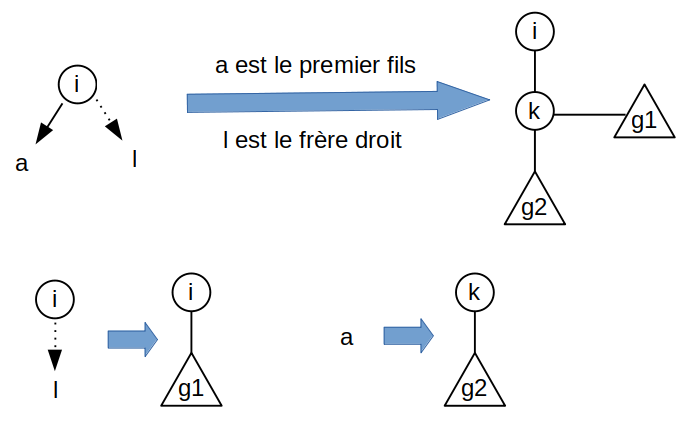
\includegraphics[scale=0.4]{Developpements/Correspondance arbres binaires et généraux/transf_gen_a_bin.png}
\end{center}
Il faut alors montrer que : \begin{enumerate}
	\item conversion est bien définie
	\item conversion N(x, .) est de la forme \lstinline|B(x, . , E )|
	\item conversion est injective
	\item \lstinline{|conversion a| = |a|}
	\item Pour \lstinline|B(x, b, E)|, $\exists$ a : conversion a = \lstinline|B(x, b, E)|
	
\end{enumerate}

Chaque preuve se fera par induction, on ne fera donc pas tout. Montrons 1 et 5. \newline

\begin{proof}Preuve de 1
	
	Montrons par induction sur la structure d'arbre que conversion a termine toujours, et renvoie quelque chose de la forme \lstinline|B( . , . , . )|.\\
	
	$\star$ Cas de bases : conversion(N(x, V)) termine et renvoie B(x, E, E) donc la propriété est vérifié.
	\begin{com}
		On peut dire ici que il n'y a pas de cas de bases pour les arbres, donc on prend le cas de bases pour les la définition des arbres en incluant celles des listes, ce qui nous fait un cas de bases pour les listes.
	\end{com}
	
	\begin{com}
		Pour justifier ce fait là, il faut pointer ce qui se passe et quel code s'exécute sur l'algorithme
	\end{com}

	$\star$ Supposons la propriété d'induction vraie pour N(x,l) et a deux arbres.
	Alors, conversion(N(x,l)) termine et est de la forme B(...) donc le premier let termine.\\
	De même, par propriété d'induction, conversion(a) termine et est de la forme B(...) donc le deuxième let termine.\\
	Donc conversion(N(x,l)) termine t renvoie B(i, B(etc...) ce qui est bien de la forme B(...).\\
	
	Ainsi par induction structurelle, conversion termine toujours.

\end{proof}

\begin{proof}Preuve de 5
	
	Montrons par induction sur la structure d'arbre binaire de b que pour tout $x \in \N$, $\exists$ a : conversion a = B($x$, b, E)
	
	$\star$ Cas de bases : soit $x \in \N$. Alors conversion N($x$, V) = B($x$, E, E). Donc la propriété est vraie sur les cas de bases\\
	
	$\star$ Soient g et d deux arbres binaires vérifiant la propriété.
	Soit $x, y\in \N$. On cherche donc a tel que conversion a = B(x, B(y, g, d), E).
	
	\begin{center}
		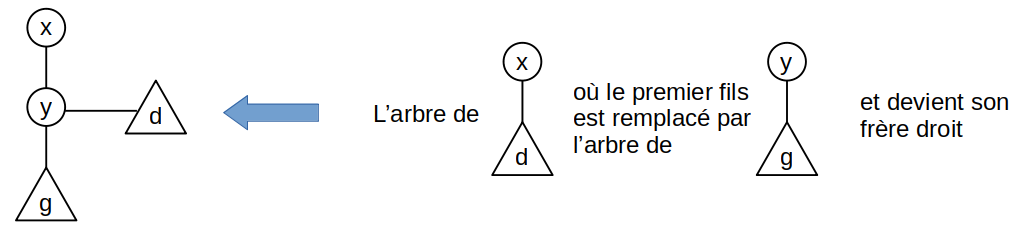
\includegraphics[scale=0.5]{Developpements/Correspondance arbres binaires et généraux/idee_surjectif.png}
	\end{center}
	
	Pa hypothèse d'induction on a qu'il existe un arbre b tel que conversion b = B(x, d, E) et il existe un arbre c tel que conversion c = B(y, g, E).\\
	
	En notant b = N($x$, l) (par 2), on a conversion(N(x, c::l) = B(x, B(y, g, d), E).
	
	\begin{com}
		La il faut montrer pourquoi quand on l'injecte dans l'algo, indéniablement, cela fonctionne, en le faisant étape par étape.
	\end{com}
	
\end{proof}

	\begin{appl}
		On peut utiliser ce code pour encoder les arbres en C par des arbres binaires.
		\begin{com}
			Expliquer à l'oral pourquoi que c'est pratique, que les parcours se font plus facilement, que l'encodage d'un arbre binaire est quand meme bien plus simple qu'un arbre générique.
		\end{com}
		En réalité, notre codage revient au codage en C où mais en plus simple.
		\begin{com}
			Le codage en C étant celui où stocke un arbre comme une valeur et un pointeur vers une liste chaînée, elle même pointant vers les arbres fils. Dans notre transformation, on élude alors le problème de la liste chaînée.
		\end{com}
		\begin{center}
			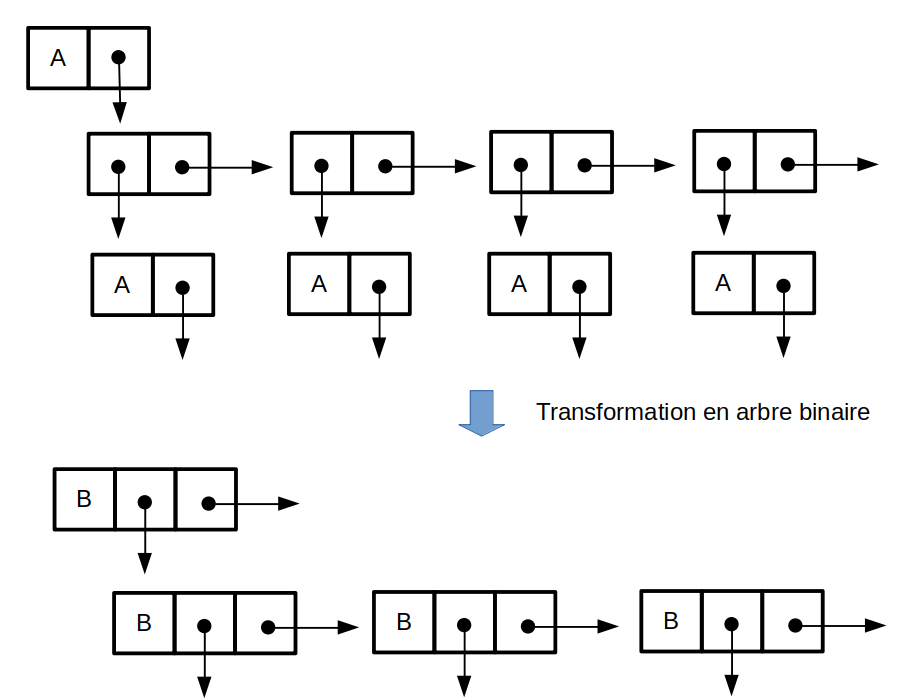
\includegraphics[scale=0.4]{Developpements/Correspondance arbres binaires et généraux/arbre_en_c.png}
		\end{center}
	\end{appl}

\chapter{Illustration du paradigme orienté objet sur la modélisation d'une personne sur une carte}\label{D32}
\dev{Emile Martinez}{}

\textit{Dans cette leçon on déroule un exemple d'utilisation de l'orienté objet, avec la modélisation et l'aspect modulaire, mais également une illustration de ce qui est fonctionnel, impératif, etc...}

\paragraph{Objectif} Représenter une personne voulant se déplacer sur une carte.

\begin{figure}
    \centering
    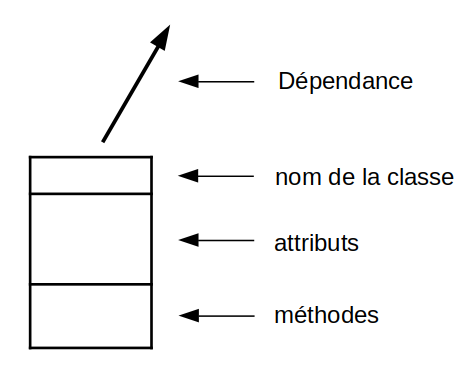
\includegraphics[scale=0.5]{Developpements/Illustration oriente objet/explication uml.png}
    \caption{Explication des champs de notre diagramme}
\end{figure}

\begin{com}
    Construire le diagramme suivant petit à petit, et ne rajouter les éléments seulement quand on en a besoin. (par exemple, la File, ne la rajouter que quand on en aura besoin)
\end{com}

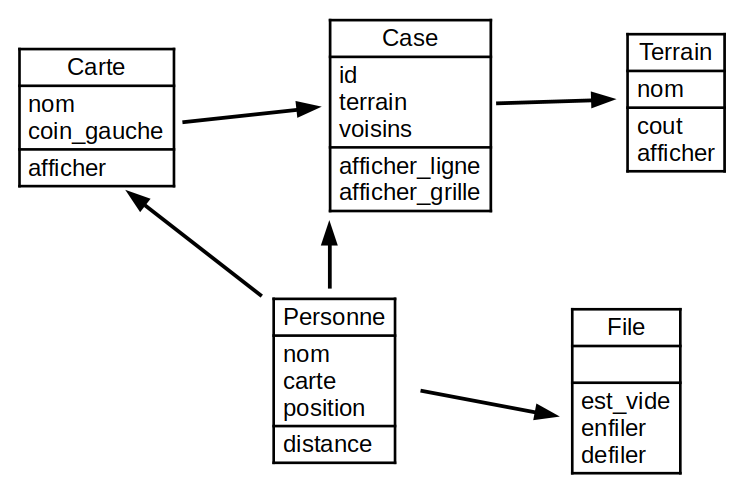
\includegraphics[scale=0.5]{Developpements/Illustration oriente objet/diagramme uml.png}

\begin{figure}
    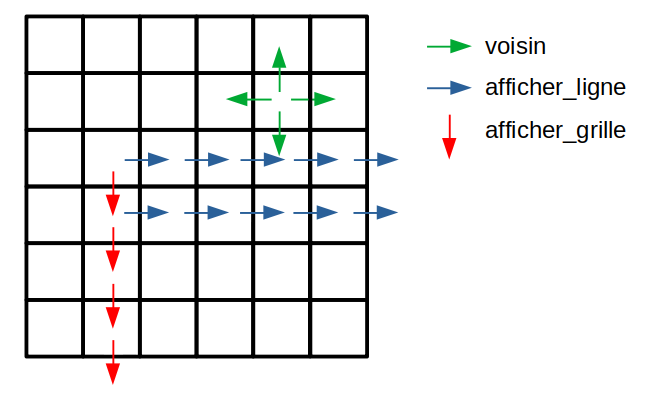
\includegraphics[scale=0.5]{Developpements/Illustration oriente objet/explication carte.png}
    \caption{Explication de la carte et du fonctionnement de afficher}
	\label{carteobj1}
\end{figure}

\begin{lstlisting}
class Carte:
    def __init__(self, ...):
        self.nom = ...
        self.coin_gauche = ...
    
    def afficher(self):
        self.coin_gauche.afficher_grille()    
\end{lstlisting}

\begin{lstlisting}
class Case:
    def __init__(self, ...):
        self.terrain = ...
    self.voisins = ... #dictionnaire de clé "haut", "gauche", etc...
    
    def afficher_ligne(self):
        self.terrain.afficher()
        if "droite" in self.voisins:
            self.voisins["droite"].afficher_ligne()
        else:
            print() # on met une nouvelle ligne
    
    def afficher_grille(self):
        self.afficher_ligne()
        if "bas" in self.voisins:
            self.voisins["bas"].afficher_grille()
\end{lstlisting}

\begin{com}
	Expliquer ici pourquoi on fait un parcours en largeur, en montrant sur la figure \ref{carteobj1} que on peut ainsi trouver un chemin en plus ou moins ligne droite pour y aller	
\end{com}

\begin{com}
	Introduire ici la nécessité d'une structure de file comme il n'en existe pas de natives intéressantes en python, et donc la rajouter au diagramme UML
\end{com}

\begin{lstlisting}
class Personne:
    def __init__(self, ...):
        self.nom = ...
        self.carte = ...
        self.position = ...
    
    def distance(self, dest):
        distance = dict()
        a_voir = File()
        a_voir.ajouter(self)
        distance[self.id] = 0
        while not a_voir.est_vide():
            c = a_voir.defiler()
            if c.id == dest:
                return distance[c.id]
            else:
                for v in c.voisins.values():
                    if v.id not in distance:
                        distance[v] = distance[c] + v.terrain.cout()
                        a_voir.enfiler(v)
        
        return -1
\end{lstlisting}

\begin{com}
	Mentionner ici l'importance de la modularité, puisque on peut alors utiliser file indépendemment de son implémentation.
\end{com}

\begin{com}
	Dire que ici cohabite le fonctionnel et l'impératif, en marquant d'une couleur les lignes récursives (celles où on affiche) et d'une autre l'impératif (l'algo de la distance)
\end{com}

\begin{com}
	Dire pour le jury que là on a écrit au tableau mais que en vrai on le projetterai écrit, et que là on a pas mis beaucoup de commentaires, la spécification, etc..., mais que en vrai évidemment dans le code on le ferait, parce que c'est très important.
\end{com}

\chapter{Approximation(s) gloutonne(s) de Indep(2)}\label{D33}
\dev{Emile Martinez}{Daphné Kany}

\textit{Cette leçon présente une (ou éventuellement 2 suivant le temps qu'on met à la faire) approximation gloutonne de Indep(2). On suppose ici la définition formelle de Indep déjà faites dans le plan de cours}

\paragraph{Instance} n tâches de durée $\omega_1, \dots \omega_n$
\paragraph{Pb} Trouver un ordonnancement sur $P_1, P_2$ qui minimise la date de fin $\tau$

\begin{algorithm}[H]
$\tau_1, \,\tau_2 \leftarrow 0$ \quad\# date de fin de $P_1,\,P_2$ \\
\Pour{i allant de $1$ à $n$}
{
	\eSi{$\tau_1 \leq \tau_2$}{
		$alloc[i] \leftarrow 1$\\
		$\sigma[i] \leftarrow \tau_1$\\
		$\tau_1 = \tau_1 + \omega_i$\\
	}{
		\#idem avec $\tau_1 \leftrightarrow \tau_2$\\
	}
}
\Retour{$\max (\tau_1, tau_2)$}
\caption{Glouton-1($w_1, \dots, w_n$)}
\end{algorithm}

\begin{proposition}
	Glouton-1 n'est pas optimal.
\end{proposition}

\begin{proof}
	Soit $I$ une l'instance $\omega_1 = \omega_2 = 1$ et $\omega_3 = 2$. On obtient alors\\
	\begin{minipage}{0.4\linewidth}
		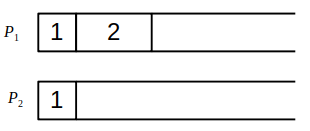
\includegraphics[scale = 0.5]{Developpements/Glouton indep 2/instance1.png} 
	\end{minipage}
	\begin{minipage}{0.4\linewidth}
		$\tau = \tau_1 = 3 \newline \tau^* = 2$
	\end{minipage}
\end{proof}

\begin{theorem}
	Glouton-1 est une $\frac{3}{2}$-approx de Indep(2)
\end{theorem}

\begin{proof}
	$\bullet$ D'abord, Glouton-1 est bien polynomial\\
	
	$\bullet$ Soit I une instance. On note $\tau$ la réponse de Glouton-1, $\tau^*$ l'optimal.
	
	Il faut alors montrer que $\dfrac{\tau}{\tau^*} \leq \dfrac{3}{2}$
	
	\paragraph{Intuition}\begin{minipage}{0.4\linewidth}
	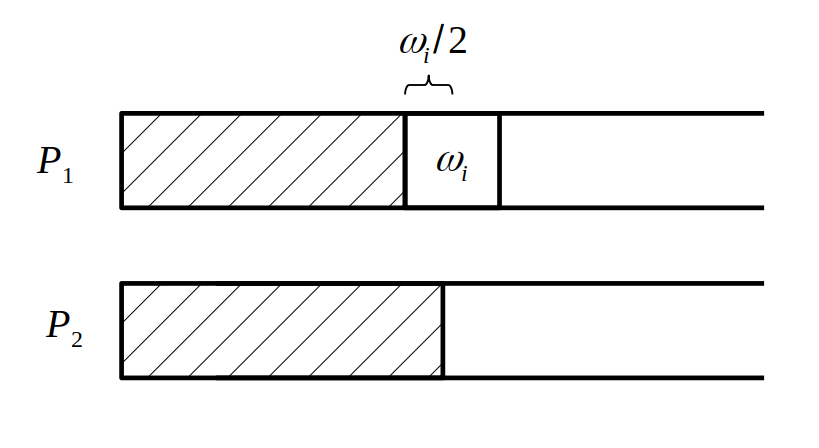
\includegraphics[scale=0.2]{Developpements/Glouton indep 2/instance2.png}\end{minipage}
	\begin{minipage}{0.4\linewidth}
		$\tau = \tau_1$ \\ $\tau^* \geq \tau - \omega_i + \frac{\omega_i}{2}$\\$ \tau \leq \frac{3\tau^*}{2}$
	\end{minipage}
	
	\begin{com}
		Ici pour expliquer, on commence par dire que on suppose que le processeur le plus occupé c'est le 1, puis on regarde la dernière tâche qu'on a mis dessus. Alors, quand on l'a mise, $P_2$ était plus avancé. Donc, ce moment là est plus grand que $\tau^*$ sans $\omega_i$. Or quand on va rajouter $\omega_i$, au mieux on pourra ne rajouter que $\frac{\omega_i}{2}$ à chacun des processeurs en réorganisant. Donc $\tau^*$ avec $\omega_i$ c'est au moins $\tau^*$ sans $\omega_i$, plus $\frac{\omega_i}{2}$, donc $\underset{\leq \tau^* \text{ sans } \omega_i}{\underbrace{\tau - \omega_i}} + \frac{\omega_i}{2}$
	\end{com}
	
	\paragraph{Preuve de l'intuition} On note $S = \sum\limits_{i = 1}^n \omega_i$
	$$\tau^* \geq \dfrac{S}{2} \qquad \circled{1}$$
	
	$$\tau_1 + \tau_2 = S \qquad \circled 2$$
	
	On considère $\tau = \tau_1$, et $\omega_i$ est la dernière tâche de $P_1$.\\
	Au moment de l'insertion de $\omega_1$ : $\underset{= \tau - \omega_i}{\underbrace{\tau_1^{(i)}}} \leq \tau^{(i)} \leq \tau^{(i)} $ \quad \circled 3\\
	
	$$\circled 3 \quad \tau_1 \leq \tau_2 - \omega_i \underset{\circled 2}{\leq} S - \tau_1 + \omega_i$$
	
	$$ 2\tau_1 \leq \underset{\leq 2\tau^* \enspace \circled 1}{\underbrace{S}} + \underset{\leq \tau^*}{\underbrace{\omega_i}} \leq 3\tau^* $$
	
\end{proof}

\begin{algorithm}[H]
	$w_1, \dots, w_n \leftarrow$ Tri($\omega_1, \dots, \omega_n$)\\
	\Retour{Glouton-1($w_1, \dots, w_n$)} 
\caption{Glouton-2($\omega_1, \dots, \omega_n$)}
\end{algorithm}

\begin{theorem}
	Glouton-2 est une $\frac{7}{6}$-approx
\end{theorem}

\begin{proof}
	On reprend la preuve de Glouton-1, mais en essayant d'améliorer $\tau^* \geq \omega_i$
	\begin{itemize}[label=$\star$]
		\item Soit $i \leq 4$, Glouton-2 est optimal\\
		$\to$ Faire tous les cas.\begin{com}
			Si il reste du temps, dire que parce que soit il faut mettre une tâche toute seule, et on le fait, soit il faut mettre la plus grande avec la plus petite, et on le fait.
		\end{com}
		\item Sinon $i \geq 5$. Alors, on a $\tau^* \geq 3 \omega_i$ (Car il y a un ruban avec 3 éléments valant au moins $\omega_i$). D'où $2\tau_1 \leq 2\tau^* + \dfrac{\tau^*}{3}$ i.e. $\tau \leq \dfrac{7}{6}\tau^*$
	\end{itemize}
\end{proof}

\paragraph{Exemple où la borne est atteinte}
Sur l'instance $\omega_1 = \omega_2 = 3$ et $\omega_3 = \omega_4 = \omega_5 = 2$, on obtient\\
	\raisebox{-0.5\height}{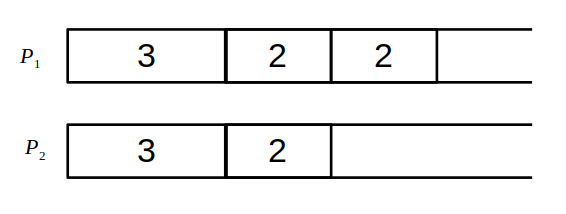
\includegraphics[scale = 0.3]{Developpements/Glouton indep 2/instance4.png}} au lieu de 
	\raisebox{-0.5\height}{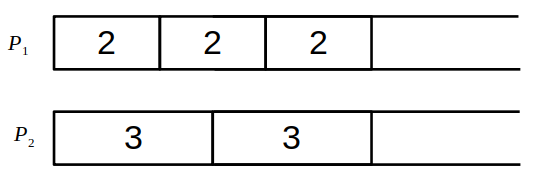
\includegraphics[scale = 0.3]{Developpements/Glouton indep 2/instance3.png}}


\begin{rem}
	Avec Glouton-2 on perd la propriété d'être en ligne. \\
	Avec Glouton-2, l'approx est mauvaise surtout pour les cas où on a peu de tâches. On pourrait alors combiner une approche exhaustive pour les premières tâches, et une approche gloutonne pour les petites.
\end{rem}

\begin{com}
	Si on a du temps, on peut aussi parler de ce qui se passe quand on a plus de processeur. On peut dire sur le dessin, que $\omega_i$ se répartit sur plus de processeurs, et donc $\tau^* \geq \tau_1 - \omega_i + \frac{\omega_i}{p}$. Ca nous fait au final une $2-\frac{1}{p}$ approx pour Glouton-1 et une $\frac{4p-1}{3p}$ pour Glouton-2
\end{com}

\chapter{Présentation de l'algorithme des k-plus proches voisins}\label{D34}
\dev{Emile Martinez}{}

\textit{Mettre une description}

\paragraph{Problème} On a des exemples $E = \{(x, c) \in X\times Y\}$ et on a $x \in X$ dont on cherche sa classe.\\
Ici $X = \mathbb R^d$

\begin{com}
	Ici on parle de $Y$, mais c'est une liste de classes.
\end{com}

\paragraph{Paramètre} $k > 0$ un entier

\begin{algo} Algorithme des $k$-plus proche voisins
	\begin{enumerate}
		\item On cherche les k plus proches voisins de $x$ dans $T$
		\item On renvoie la classe majoritaire parmi ces $k$ classes
	\end{enumerate}
\end{algo}

\begin{example}
	Imaginons qu'on ait un capteur permettant de détecter le poids d'un animal qui passe et sa taille. Comment savoir quel animal était-ce ?\\ \centering
	\includegraphics[scale=0.4]{Developpements/k voisins/graphe.png}
\end{example}

\paragraph{Question} Quel choisir k ?

\begin{com}
	Si $k$ est trop petit.
\end{com}
\begin{center}
	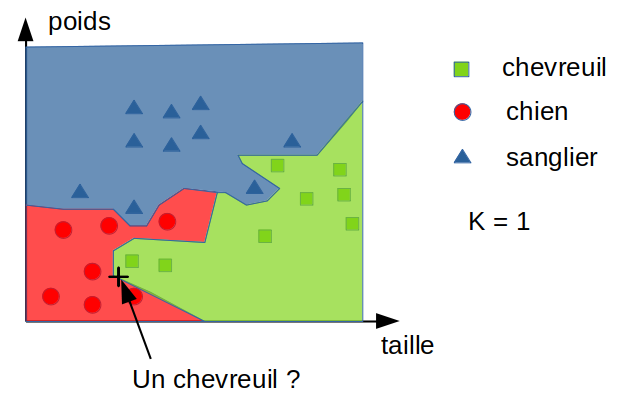
\includegraphics[scale=0.4]{Developpements/k voisins/graphe2.png}
\end{center}

$\to$ On a une trop grande influence des cas particuliers $\to$ sur apprentissage.

Exemple classique de sur apprentissage quand on veut approximer des points par une courbe : \\
\begin{minipage}{0.5\linewidth}
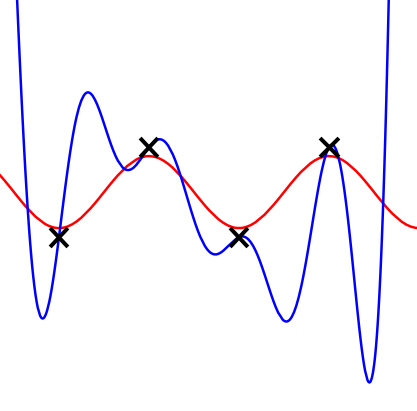
\includegraphics[scale=0.4]{Developpements/k voisins/sur_apprentissage.png}
\end{minipage}\begin{minipage}{0.5\linewidth}
La ligne bleue colle mieux aux données mais à l'air moins bien que la rouge.
\end{minipage}

\paragraph{Influence lointaine} Si $K$ est choisi trop grand, des points trop loin auront une trop grande influence.
\begin{center}
	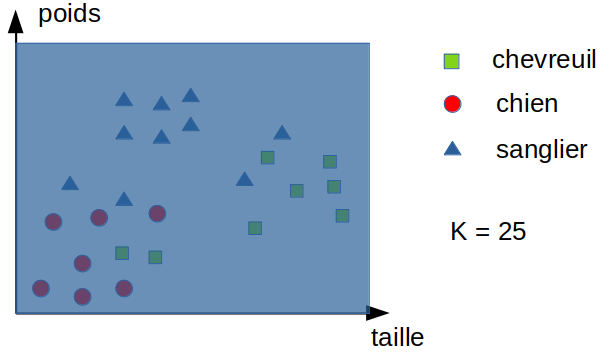
\includegraphics[scale=0.4]{Developpements/k voisins/graphe3.png}	
\end{center}

\begin{com}
	Super il faut le choisir bien, mais ca nous dit pas comment. 
\end{com}

\paragraph{Comment le choisir ?} On en essaie plein.\\
On sépare $E$ en $D_A$ et $D_T$ (avec $\dfrac{\left| D_A \right|}{|E|} \simeq 80\%$). On essaye alors de prédire $D_T$ en utilisant $D_A$ et on regarde pour quel $k$ on a la meilleur performance.

\paragraph{Question} Pourquoi séparer ?\\
$\to$ Car si on faisait sur les mêmes éléments, on éviterait pas le biais du surapprentissage.
\begin{com}
	Ici revenir sur l'exemple pour le montrer. En disant que avec $k =1$ on aurait $100\%$ de réussite.
\end{com}

\paragraph{Validation croisée} Si on a pas assez de données ?
\begin{com}
	Chaque donnée joue alternativement le rôle de données de test et de données d'entrainement.
\end{com}
\includegraphics[scale=0.4]{Developpements/k voisins/validation_croisee.png}


\paragraph{Complexité} Comment chercher les $K$ plus proches voisins parmi $N$ points ?
	\begin{itemize}[label=$\bullet$]
		\item En cherchant pour $i$ allant de $1$ à $K$ le point le plus proche puis en l'enlevant.
			\\ $\to O(N\times K)$ 
		\item En parcourant les $N$ points et en gardant à chaque fois les $K$ plus proches (quand on en trouve un plus petit, on enlève le plus loin parmi les $K$).
			\\ $\to O(N \times \log K)$ si on utilise les structures de données adéquates
		\item En faisant des pré-calculs, on peut obtenir une structure permettant de faire la recherche des $K$ plus proche voisins en $O(\log N + K)$ en moyenne. $\to$ rentable pour beaucoup de recherche.
		\begin{com}
			Faire l'analogie avec la dimension $1$ et les listes triées.
		\end{com}
	\end{itemize}

\paragraph{Notion de distance} On utilise ici la distance euclidienne mais on pourrait également utiliser d'autres distances, comme la distance de Manhattan.

\paragraph{Normalisation des paramètres} Il se peut qu'une coordonnée soit beaucoup plus grande que toutes les autres et ait beaucoup trop d'importances. Et même, quand on compare des grandeurs différentes, comment choisir l'unité que l'on prend (influençant le poids de cette grandeur)

\begin{center}
	\includegraphics[scale=0.5]{Developpements/k voisins/decale.png}
\end{center}




\chapter{Validité de la construction d'un ensemble inductif}\label{D35}
\dev{Emile Martinez}{}

\textit{Ce développement présente le fait qu'une construction inductive est valide. Il consiste à démontrer qu'on peut définir seulement le nom des fonctions et qu'on arrivera à en faire quelque chose. Puis l'équivalence des définitions par le haut et par le bas. On se place dans un contexte où on dit que les constructeur sont de $X^{\alpha(i)}$ dans $X$, injectif et d'image disjointes. Si on le met dans le leçon principe d'induction, on niveau MPII, il faut dire que c'est à la fin du cours, on fait ça pour ceux qui veulent suivre en distribuant un poly et en faisant ça au tableau. Avec notamment le fait que c'est la meme chose que ce qu'on écrit, et que ce qu'affiche OcamL (d'où le fait de le faire après OcamL)}

\begin{definition}Quelques défintions pour commencer\\
	$\Sigma =  $ $[$'a' - 'z'$]$ \qquad $\Gamma = \Sigma \cup \{$'[', ']', '\#' $\}$\\
	$\Sigma^* = \bigcup\limits_{n \in \N} \Sigma^n$ \qquad $\Gamma^* = \bigcup\limits_{n \in \N} \Gamma^n$ \\
	On définit également $\cdot :\begin{array}{cll}
	\Gamma^* \times \Gamma^* & \to & \Gamma^*\\
	(u,v) & \mapsto & (u_1, \, \dots, \, u_{|u|}, \, v_1, \, \dots, \, v_{|v|})
	\end{array}$
\end{definition}

\begin{rem}
	$\cdot(\Sigma^n \times \Sigma^m) = \Sigma^{n+m}$
\end{rem}

\begin{com}
	Dire que 'a', 'b', ..., '[' c'est vraiment simplement des symboles mathématiques différents les uns des autres. Que la puissance $n$ c'est les suites finies, donc on prend l'ensemble des suites finies. La définition de la concaténation on peut la rajouter dans les def après le paragraphe suivant
\end{com}

\paragraph{De quoi on part} Au début, on a seulement les noms des élements de la signature $\left( \mathcal B, \left(f_i\right)_{i \in I} \right) $: 
$$\mathcal{B} \subset \Sigma^* \qquad \forall i \in I, \, \left\{ \begin{array}{l}
nom_i \in \Sigma^* \\ nom_i \notin \mathcal{B} \\ nom_i \neq nom_j \text { pour } j \neq i
\end{array} \right.$$

\paragraph{Construction de nos ensembles}

Pour $X$ on va prendre $\Gamma^*$.\\

$\mathcal B = \mathcal B \subset \Sigma^* \subset \Gamma^*$\\

$f_i : \begin{array}{cll}
	\Gamma^{\alpha(i)} & \to & \Gamma^*\\
	(u_1, \, \dots, \, u_{\alpha(i)}) & \mapsto & nom_i \cdot \text [ \cdot u_1 \cdot \# \cdot  ... \cdot \# \cdot u_{\alpha(i)} \cdot \text ]
\end{array}$\\

\begin{rem}
\textbf{Qu'est-ce que c'est ce truc ?}

C'est ce que l'on fait quand on écrit l'enchainement des constructeurs et qu'il n'y a pas d'ambiguïté. C'est la même chose que fait OcamL, quand dans l'interpréteur il vous affiche un objet construit par des constructeurs :\\\\
\begin{minipage}{0.5\linewidth}
	\begin{lstlisting}
type bin = E | B of bin*int*bin;;
ajout (ajout (ajout E 1) 2) 3;;
\end{lstlisting}
\end{minipage} \enspace $\to$ \enspace \begin{minipage}{0.4\linewidth}
\begin{lstlisting}
- : bin = B (B (E, 1, E),
2, B (E, 3, E))
\end{lstlisting}
\end{minipage}\\que nous on note $B[B[E\#1\#E]\#2\#B[E\#3\#E]]$
\end{rem}
$\bullet$ $$\begin{array}{cl}
 f_i(u_1, \dots, u_{\alpha(i)}) = f_j(v_1, \dots, v_{\alpha(j)})  \\
 \Downarrow \\
  nom_i \cdot \text [ \cdot u_1 \cdot \# \cdot  ... \cdot \# \cdot u_{\alpha(i)} \cdot \text ] = nom_j \cdot \text [ \cdot u_1 \cdot \# \cdot  ... \cdot \# \cdot u_{\alpha(j)} \cdot \text ] \\
  \Downarrow *\\
  nom_i = nom_j \\ \Downarrow \\ i = j
\end{array}$$

$* [  \, \notin nom_i \text{ et }  [ \, \notin nom_j \text{ donc le premier [ est celui après } nom$

Donc pour $i \neq j$, $Im(f_i) \cap Im(f_j) = \emptyset$\\

$\bullet$
$$
\forall b \in \mathcal B, \forall i, \, \forall u_1, \, \dots, u_{\alpha(i)} \in \Gamma^*, \left\{ \begin{array}{l}
	[ \in f_i(u_1, \, u_{\alpha(i)}) \\ [ \notin b
\end{array}\right. \implies b \neq f_i(u_1,\, \dots, \, u_{\alpha_i})
$$

$\bullet$ Reste l'injectivité des $f_i$. Mais en fait elles ne sont pas injectives.

\begin{com}
	Là on peut dire que en fait il faudrait modifier légèrement X, mais la construction des $f_i$ est la même, et c'est simplement technique. On peut également mentionner à l'attention du jury que ca ferait un super sujet pour plus tard en MPI.
\end{com}

\paragraph{Définition de l'ensemble inductif} Maintenant qu'on a l'existence de nos constructeurs, il faut savoir si notre définition des ensembles inductifs est correctes.

\begin{com}
	Dans la leçon, on aurait la définition de $T_0 = \mathcal B$ et $T_{k+1} = T_k \cup \bigcup\limits_{i \in I} f_i\left(T_k^{\alpha(i)}\right)$
\end{com}

Notons $P_S$ la propriété défini sur $\mathcal P(X)$ $P_S(A) : \mathcal B \subset A \text{ et } \forall i \in I, \, f_i\left( A^{\alpha(i)} \right) \subset A$

\begin{com}
	$P_S$ veut dire contient $\mathcal B$ et stable par tous les $f_i$
\end{com}

Prenons comme définition de l'ensemble inductif $E$ défini par la signature $(\mathcal B, (f_i)_{i \in I})$, le plus petit ensemble contenant $\mathcal B$ et stable par tous les $f_i$.

\begin{itemize}[label=$\star$]
	\item Premièrement, cet ensemble existe-t-il ?

	Oui. J'annonce même que c'est $\bigcap\limits_{\substack{A \in \mathcal P(X) \\ P_S(A)}} A$.
	
	En effet,\begin{itemize}[label=$\bullet$]
		\item $\left(\forall A \in \mathcal P(X), P_S(A) \implies \mathcal B \subset A \right) \implies \mathcal B \subset \bigcap\limits_{\substack{A \in \mathcal P(X) \\ P_S(A)}} A$
		
		\item Soit $i\in I$, soit $x_1, \, \dots, \, x_{\alpha(i)} \in \bigcap\limits_{\substack{A \in \mathcal P(X) \\ P_S(A)}} A$.\\
		Alors $\forall A \in \mathcal P(X), P_S(A) \implies \left\{ \begin{array}{l}
		P_S(A) \\ x_1, \dots, x_{\alpha(i)} \in A 
		\end{array}\right.\implies f_i\left(x_1, \dots, x_{\alpha(i)}\right) \in A$\\
		Donc $\bigcap\limits_{\substack{A \in \mathcal P(X) \\ P_S(A)}} A$ est stable par tous les $f_i$
		
		\item Soit $A \in \mathcal P(x)$ tel que $P_S(A)$. Alors, $\bigcap\limits_{\substack{A \in \mathcal P(X) \\ P_S(A)}} A \subset A$.
		
	\end{itemize}
	Ainsi, $\bigcap\limits_{\substack{A \in \mathcal P(X) \\ P_S(A)}} A$ est bien le plus petit ensemble vérifiant $P_S$.
	\begin{com}
		Si on manque de temps pendant le développement, on peut ne pas faire cette preuve.
	\end{com}

	Reste maintenant à montrer que $E = \bigcup\limits_{k \geq 0} T_k$
	
	\item $\boxed{\subset}$ 
		\begin{itemize}[label=$\bullet$]
			\item $\mathcal B = T_o \subset \bigcup\limits_{k \geq 0} T_k$
			\item Soit $i \in I$ et $x_1, \, \dots, \, x_{\alpha(i)} \in \bigcup\limits_{k \geq 0} T_k$\\
			Alors par définition, $\forall j \in \llbracket 1, \alpha(i) \rrbracket , \, \exists k_j \in \N : \: x_j \in T_{k_j}$\\
			Posons $K = \max\limits_j k_j$\\
			Alors, comme $T_k \subset T_{k'}$ pour $k \leq k'$ (par une récurrence immédiate par définition des $T_k$), $\forall j \in \llbracket 1, \alpha(i) \rrbracket, \, x_j \in T_K $. Donc par définition de $T_{K+1}$, $f_i(x_1, \, \dots, \, x_{\alpha(i)}) \in T_{K+1} \subset  \bigcup\limits_{k \geq 0} T_k$
			Ainsi, $\bigcup\limits_{k \geq 0} T_k$ est stable par tous les $f_i$
		\end{itemize}

	D'où $P_S\left( \bigcup\limits_{k \geq 0} T_k\right)$, donc par définition de $E$, $E \subset \bigcup\limits_{k \geq 0} T_k$
	
	
	\item $\boxed{\supset}$ Soit $\mathcal P$ la propriété défini pour $k \in \N$ par $\mathcal P(k): \: « T_k \subset E »$
	\begin{itemize}[label=$\bullet$]
		\item Par définition de $E$, $T_0 = \mathcal B \subset E$ d'où $\mathcal P(0)$.
		\item Soit $k \in \N$ tel que $\mathcal P(k)$. Soit $y \in T_{k+1}$. Alors par définition de $T_{k+1}$ on a deux possibilités :
		\begin{itemize}
			\item Si $y \in T_k$ alors par $\mathcal P(k)$, $y \in E$
			\item Si $\exists i \in I :\: \exists x_1, \, \dots, \, x_{\alpha(i)} \in T_k : \: y = f_i\left(x_1, \,\dots, \, x_{\alpha(i)}\right) $\\
			Donc par $\mathcal P (k)$, $\forall j \in \llbracket 1, \alpha(i) \rrbracket,\, x_i \in E$. Or $E$ est stable par tous les $f_i$ donc $y = f_i\left(x_1, \,\dots, \, x_{\alpha(i)}\right) \in E$.
		\end{itemize}
		D'où $\forall y \in T_{k+1}, \, y\in E$, soit $\mathcal P(k+1)$.
	\end{itemize}
	Ainsi par principe de récurrence, $\forall k \in \N, T_k \subset E$, donc $ \bigcup\limits_{k \geq 0} T_k \subset E$.
\end{itemize}



%\chapter{Je sais pas encore}\label{Dbeaucoup}
%\dev{Emile Martniez}{}

\begin{definition} CFG
	\begin{itemize}
		\item $\Sigma$ fini
		\item $V$ fini($\Sigma \cap V = \emptyset$)
		\item $\mathcal R \subset V\times \left(\Sigma \cup V\right)^*$ (noté $\to$)
		\item $\S_0 \in V$
	\end{itemize}
\end{definition}

\begin{example}
	$\mathcal G : S \to aSb | \epsilon, \, \mathcal L_{\mathcal G}(S) =\left\{a^nb^n | n\in \N\right\}$
\end{example}

\begin{proposition}
	\begin{itemize}
		\item $\mathcal L_{\mathcal G}(S)$ est décidable (HP)
		\item $\epsilon \in \mathcal L_{\mathcal G}(S)$ est décidable
	\end{itemize}
\end{proposition}

\begin{proof}
	$$
	W_0 = \left\{ S \in V | S\to \epsilon\right\} \\
	W_{n+1} = W_0 \cup \left\{S \in V | S \to w, w \in \right\}
	$$
\end{proof}

\chapter{Preuve de l'équilibrage des arbres rouges noirs et méthode d'insertion}\label{D36}
\dev{Emile Martinez}{Daphné Kany}

\textit{On estime que la définition des ARN est déjà admise}.

\paragraph{Insertion dans un ABR} 
\begin{enumerate}
	\item On colorie la racine en noir
	\item On insert le noeud en tant que feuille comme dans un ABR \\
	On le colore en rouge
	\item On rétablit la propriété (ii) par rotations successives en préservant la hauteur noire.
\end{enumerate}

\begin{definition}Rotation\\ 
	\begin{tabular}{ccc}
		\multirow{5}{*}{
		\begin{tikzpicture}[-, node distance=1cm]
			\node[state, scale=0.5] (q0) {$k_3$};
			\node[state, below left of = q0, scale=0.5] (q1) {$k_2$};
			\node[below left of =q1] (q2) {$t_1$};
			\node[below right of = q1] (q3) {$t_2$};
			\node[below right of = q0] (q4) {$t_3$};
			\draw (q0) edge[] node{} (q1) ;
			\draw (q1) edge[] node{} (q2) ;
			\draw (q1) edge[] node{} (q3) ;
			\draw (q0) edge[] node{} (q4) ;
		\end{tikzpicture}} &  &
		\multirow{5}{*}{\begin{tikzpicture}[-, node distance=1cm]
			\node[state, scale=0.5] (q0) {$k_2$};
			\node[state, below right of = q0, scale=0.5] (q1) {$k_3$};
			\node[below left of =q0] (q2) {$t_1$};
			\node[below left of = q1] (q3) {$t_2$};
			\node[below right of = q1] (q4) {$t_3$};
			\draw (q0) edge[] node{} (q1) ;
			\draw (q0) edge[] node{} (q2) ;
			\draw (q1) edge[] node{} (q3) ;
			\draw (q1) edge[] node{} (q4) ;
		\end{tikzpicture}} \\ & $\overset{\text{rotation droite }(k_3)}{\longrightarrow}$ & \\  & $\underset{\text{rotation gauche } (k_2)}{\longleftarrow} $ &
	\end{tabular}
\end{definition}
\begin{rem}
	La rotation préserve la structure d'ABR
\end{rem}

\begin{com}
	Expliquer la remarque à l'oral sur le dessin de la définition
\end{com}

\paragraph{Etape 3 de l'insertion}
4 cas à considérer :
%\begin{enumerate}
%	\item \raisebox{-0.5\height}{\begin{tikzpicture}[-, node distance=1cm]
%		\node[state, black, scale=0.5] (q0) {$k_3$};
%		\node[state, below left of = q0, red, scale=0.5] (q1) {$k_2$};
%		\node[state, below left of = q1, red, scale=0.5] (q2) {$x$};
%		\node[below left of =q2] (q3) {$t_0$};
%		\node[below right of = q2] (q4) {$t_1$};
%		\node[below right of = q1] (q5) {$t_2$};
%		\node[below right of = q0] (q6) {$t_3$};
%		
%		
%		\draw (q0) edge[] node{} (q1) ;
%		\draw (q1) edge[] node{} (q2) ;
%		\draw (q2) edge[] node{} (q3) ;
%		\draw (q2) edge[] node{} (q4) ;
%		\draw (q1) edge[] node{} (q5) ;
%		\draw (q0) edge[] node{} (q6) ;
%	\end{tikzpicture}}
%
%	\item \raisebox{-0.5\height}{\begin{tikzpicture}
%		\node[state, black, scale=0.5] (q0) {$k_3$};
%		\node[state, below left of = q0, red, scale=0.5] (q1) {$k_2$};
%		\node[state, below right of = q1, red, scale=0.5] (q2) {$x$};
%		\node[below left of =q2] (q3) {$t_0$};
%		\node[below right of = q2] (q4) {$t_1$};
%		\node[below left of = q1] (q5) {$t_2$};
%		\node[below right of = q0] (q6) {$t_3$};
%		
%		
%		\draw (q0) edge[] node{} (q1) ;
%		\draw (q1) edge[] node{} (q2) ;
%		\draw (q2) edge[] node{} (q3) ;
%		\draw (q2) edge[] node{} (q4) ;
%		\draw (q1) edge[] node{} (q5) ;
%		\draw (q0) edge[] node{} (q6) ;
%	\end{tikzpicture}}
%
%	\item Pareil
%	\item Pareil\\
%\end{enumerate}

\begin{enumerate}
	\item \raisebox{-0.5\height}{\begin{tikzpicture}[-, node distance=1cm]
		\node[state, black, scale=0.5] (q0) {$k_3$};
		\node[state, below left of = q0, red, scale=0.5] (q1) {$k_2$};
		\node[state, below left of = q1, red, scale=0.5] (q2) {$x$};
		\node[below left of =q2] (q3) {$t_0$};
		\node[below right of = q2] (q4) {$t_1$};
		\node[below right of = q1] (q5) {$t_2$};
		\node[below right of = q0] (q6) {$t_3$};
		
		
		\draw (q0) edge[] node{} (q1) ;
		\draw (q1) edge[] node{} (q2) ;
		\draw (q2) edge[] node{} (q3) ;
		\draw (q2) edge[] node{} (q4) ;
		\draw (q1) edge[] node{} (q5) ;
		\draw (q0) edge[] node{} (q6) ;
	\end{tikzpicture}} $\overset{\text{Rotation droite } (k_3)}{\longrightarrow} $ \raisebox{-0.5\height}{\begin{tikzpicture}[-, node distance=1cm]
		\node[state, red, scale=0.5] (q0) {$k_2$};
		\node[state, below right = 0.5 cm and 0.8 cm of q0, black, scale=0.5] (q1) {$k_3$};
		\node[state, below left = 0.5 cm and 0.8 cm of q0, black, scale=0.5] (q2) {$x$};
		\node[below left of =q2] (q3) {$t_0$};
		\node[below right of = q2] (q4) {$t_1$};
		\node[below left of = q1] (q5) {$t_2$};
		\node[below right of = q1] (q6) {$t_3$};
		
		\draw (q0) edge[] node{} (q1) ;
		\draw (q0) edge[] node{} (q2) ;
		\draw (q2) edge[] node{} (q3) ;
		\draw (q2) edge[] node{} (q4) ;
		\draw (q1) edge[] node{} (q5) ;
		\draw (q1) edge[] node{} (q6) ;
	\end{tikzpicture}}
	
	\item \raisebox{-0.5\height}{\begin{tikzpicture}
		\node[state, black, scale=0.5] (q0) {$k_3$};
		\node[state, below left of = q0, red, scale=0.5] (q1) {$k_2$};
		\node[state, below right of = q1, red, scale=0.5] (q2) {$x$};
		\node[below left of =q2] (q3) {$t_0$};
		\node[below right of = q2] (q4) {$t_1$};
		\node[below left of = q1] (q5) {$t_2$};
		\node[below right of = q0] (q6) {$t_3$};
		
		
		\draw (q0) edge[] node{} (q1) ;
		\draw (q1) edge[] node{} (q2) ;
		\draw (q2) edge[] node{} (q3) ;
		\draw (q2) edge[] node{} (q4) ;
		\draw (q1) edge[] node{} (q5) ;
		\draw (q0) edge[] node{} (q6) ;
	\end{tikzpicture}} $\overset{\text{Rotation gauche }(k_2)}{\longrightarrow}$ \raisebox{-0.5\height}{\begin{tikzpicture}[-, node distance=1cm]
	\node[state, black, scale=0.5] (q0) {$k_3$};
	\node[state, below left of = q0, red, scale=0.5] (q1) {$x$};
	\node[state, below left of = q1, red, scale=0.5] (q2) {$k_2$};
	\node[below left of =q2] (q3) {$t_2$};
	\node[below right of = q2] (q4) {$t_0$};
	\node[below right of = q1] (q5) {$t_1$};
	\node[below right of = q0] (q6) {$t_3$};
	
	
	\draw (q0) edge[] node{} (q1) ;
	\draw (q1) edge[] node{} (q2) ;
	\draw (q2) edge[] node{} (q3) ;
	\draw (q2) edge[] node{} (q4) ;
	\draw (q1) edge[] node{} (q5) ;
	\draw (q0) edge[] node{} (q6) ;
\end{tikzpicture}} $ \overset{\text{Etape 1}}{\rightarrow}$
	\item Pareil
	\item Pareil
\end{enumerate}

\paragraph{Invariant}\begin{itemize}
	\item On a toujours au plus, en tout, 2 noeuds rouges consécutifs
	\item La hauteur noire est préservée
\end{itemize}

\begin{example}
	\raisebox{-0.5\height}{\begin{tikzpicture}[-, node distance=1cm]
		\node[state, black, scale=0.5] (q0) {1};
		\node[state, black, below left of = q0, scale=0.5] (q1) {0};
		\node[state, red, below right of = q0, scale=0.5] (q2) {3};
		\node[state, black, below left of = q2, scale=0.5] (q3) {2};
		\node[state, black, below right of = q2, scale=0.5] (q4) {4};
		\node[state, red, below right of = q4, scale=0.5] (q5) {6};
		\node[state, red, below left of = q5, scale=0.5] (q6) {5};
		
		
		\draw (q0) edge[] node{} (q1) ;
		\draw (q0) edge[] node{} (q2) ;
		\draw (q2) edge[] node{} (q3) ;
		\draw (q2) edge[] node{} (q4) ;
		\draw (q4) edge[] node{} (q5) ;
		\draw (q5) edge[] node{} (q6) ;
		
	\end{tikzpicture}} $\overset{\text{Rotation\_droite(6)}}{\longrightarrow}$
	\raisebox{-0.5\height}{\begin{tikzpicture}[-, node distance=1cm]
		\node[state, black, scale=0.5] (q0) {1};
		\node[state, black, below left of = q0, scale=0.5] (q1) {0};
		\node[state, red, below right of = q0, scale=0.5] (q2) {3};
		\node[state, black, below left of = q2, scale=0.5] (q3) {2};
		\node[state, black, below right of = q2, scale=0.5] (q4) {4};
		\node[state, red, below right of = q4, scale=0.5] (q5) {5};
		\node[state, red, below right of = q5, scale=0.5] (q6) {6};
		
		
		\draw (q0) edge[] node{} (q1) ;
		\draw (q0) edge[] node{} (q2) ;
		\draw (q2) edge[] node{} (q3) ;
		\draw (q2) edge[] node{} (q4) ;
		\draw (q4) edge[] node{} (q5) ;
		\draw (q5) edge[] node{} (q6) ;
		
	\end{tikzpicture}} \\
	$\overset{\text{Rotation\_gauche(4)}}{\longrightarrow}$  \raisebox{-0.5\height}{\begin{tikzpicture}[-, node distance=1cm]
		\node[state, black, scale=0.5] (q0) {1};
		\node[state, black, below left of = q0, scale=0.5] (q1) {0};
		\node[state, red, below right of = q0, scale=0.5] (q2) {3};
		\node[state, black, below left of = q2, scale=0.5] (q3) {2};
		\node[state, red, below right of = q2, scale=0.5] (q4) {5};
		\node[state, black, below left of = q4, scale=0.5] (q5) {4};
		\node[state, black, below right of = q4, scale=0.5] (q6) {6};
		
		
		\draw (q0) edge[] node{} (q1) ;
		\draw (q0) edge[] node{} (q2) ;
		\draw (q2) edge[] node{} (q3) ;
		\draw (q2) edge[] node{} (q4) ;
		\draw (q4) edge[] node{} (q5) ;
		\draw (q4) edge[] node{} (q6) ;
		
	\end{tikzpicture}}
	$\overset{\text{Rotation\_gauche(1)}}{\longrightarrow}$
\raisebox{-0.5\height}{\begin{tikzpicture}[-, node distance=1cm]
	\node[state, red, scale=0.5] (q0) {3};
	\node[state, black, below left = 0.5cm and 0.8cm of q0, scale=0.5] (q1) {1};
	\node[state, black, below right = 0.5cm and 0.8cm of q0, scale=0.5] (q2) {5};
	\node[state, black, below left of = q1, scale=0.5] (q3) {0};
	\node[state, black, below right of = q1, scale=0.5] (q4) {2};
	\node[state, black, below left of = q2, scale=0.5] (q5) {4};
	\node[state, black, below right of = q2, scale=0.5] (q6) {6};
	
	
	\draw (q0) edge[] node{} (q1) ;
	\draw (q0) edge[] node{} (q2) ;
	\draw (q1) edge[] node{} (q3) ;
	\draw (q1) edge[] node{} (q4) ;
	\draw (q2) edge[] node{} (q5) ;
	\draw (q2) edge[] node{} (q6) ;
	
\end{tikzpicture}}

\end{example}

\paragraph{Complexité :} \begin{enumerate}
	\item $O(h)$
	\item $O(h)$
	\item $O(1)$
\end{enumerate}


\begin{proposition}
	Soit $A$ un ARN de hauteur $h$ à $n$ noeuds, alors $h = O(\log n)$
\end{proposition}

\begin{lemma}
	Soit $A$ un ARN. Alors :\begin{enumerate}
		\item $h \leq 2 h_N $ où $h_N$ est la hauteur noire.
		\item $2^{h_N} \leq n+1$
	\end{enumerate}
\end{lemma}

\begin{proof}
	\begin{enumerate}
		\item Soit $C$ un chemin de la racine à une feuille de longueur $h$.
		
		On note $h_R(C)$ le nombre de noeuds rouges de $C$ et $h_N(C)$ le nombre de noeuds noirs de $C$.
		
		$|C| = h = h_R(C) + h_N(C)$.\\ \\
		D'après (ii) (de la def) : $h_R(C) \leq h_N(C)$
		D'après (iii) : $h_N(C) = h_N$.\\
		
		Donc, $h \leq 2 h_N$.
		
		\item Procédons par induction
		\begin{com}
			Si on a pas le temps ici on écrit simplement induction.
		\end{com}
		\begin{itemize}[label = $\star$]
			\item Si l'arbre est vide, le résultat est immédiat.
			\item Soit $\mathcal A$ un ARN dont les deux fils $\mathcal A_g$ et $\mathcal A_d$ vérifient la propriété (ce sont bien des ARN).
			Alors, \begin{itemize}
				\item Si la racine de $\mathcal A$ est rouge, $2^{h_N(\mathcal A)} = 2^{h_N(\mathcal A_g)} \leq \left| \mathcal A_g \right| +1 \leq \left| \mathcal A \right| + 1$
				\item Si la racine de $\mathcal A$ est noire, alors $2^{h_N(\mathcal A)} = 2^{h_N(\mathcal A)-1} + 2^{h_N(\mathcal A)-1} = 2^{h_N(\mathcal A_g)} + 2^{h_N(\mathcal A_d)} \underset{\text{HI}}{\leq} \underset{= \left| \mathcal A \right|}{\underbrace{\left| \mathcal A_g \right| + 1 + \left|\mathcal A_d\right|}} + 1 $
			\end{itemize}
		\end{itemize}
	\end{enumerate}
\end{proof}

Ainsi, $h_N \leq \log (n+1)$ donc $h \leq 2 \log(n+1)$. Donc h = $O(\log n)$\\

Insertion : $O(\log n)$



\chapter{Généralisation du tri par comptage à l'aide de dictionnaires}\label{D37}
\dev{Emile Martinez}{Emile Martinez, Daphné Kany, sur une idée influencé par chat GPT}

\begin{algorithm}[H]
	\Entree{Un tableau $T$ d'entiers positifs\\ $|T| = n$}
	\Sortie{$T$ trié}
	
	$N \gets max(T)$ \# $O(n)$\\
	$T2 \gets$ tableau de taille $N+1$ initialisé à $0$.\\
	\Pour{$x$ dans $T$}{
		$T2[x] \gets T2[x] + 1$\\
	}
	$indice \gets 0$\\
	\Pour{$i$ de $0$ à $N$}{
		\Pour{$j$ de $0$ à $T2[i]$}{
			$T[indice] \gets i$\\
			$indice \gets indice + 1$\\
		}
	}
	\Retour{$T$}
	\caption{Tri par comptage}
\end{algorithm}

\begin{example}
	$T = [2, 1, 5, 1, 2]$\\
	$N = 5$\\
	$T2 = [0, 2, 2, 0, 0, 1]$\\
\end{example}

\begin{rem}
	Complexité spatiale : $O(N)$\\
	Complexité temporelle : $O(n+N)$\\
	\begin{com}
		Dire que si $N$ vaut 500 000 000 on l'a dans le 
	\end{com}
	Ce tri n'est pas en place.
\end{rem}


\paragraph{Problème :} Comment généraliser cet algorithme pour des tableaux contenant d'autres valeurs ?

\begin{algorithm}[H]
	\Entree{Un tableau $T$ d'entiers \textcolor{red}{/ Un tableau $T$ d'éléments de $E$} \textcolor{red}{d'éléments de $E$} \\ \textcolor{red}{Une fonction $f : E \to \N$}}
	\Sortie{$T$ trié}
	$d \gets$ dictionnaire vide\\
	\Pour{$x$ dans T}{
		$i \gets$ $recherche(d, x)$ \textcolor{red}{/ $l \gets$ $recherche(d, f(x))$}\\
		\eSi{$l \neq None$}{
			\textcolor{red}{Ajouter $x$ à $l$}\\
			$Insertion(d, x, i+1)$ \textcolor{red}{/ $Insertion(d, f(x), l)$}\\
		}{
			$Insertion(d, x, 1)$ \textcolor{red}{/ $Insertion(d, f(x), [x])$}\\
		}
	}
	$T2 = []$\\
	\Pour{$k$ dans $d$}{
		Ajouter $k$ à $T2$\\
	}
	Trier $T2$\\
	$indice \gets 0$\\
	\Pour{$i$ dans $T_2$}{
		$k \gets recherche(d, i)$ \textcolor{red}{/ $l \gets recherche(d, i)$}\\
		\Pour{$j$ de $0$ à $k-1$ \textcolor{red}{/ $x \in l$}}{
			$T[indice] \gets i$ \textcolor{red}{/ $T[indice] \gets x$}\\
			$indice \gets indice + 1$
		}
	}
	\caption{Généralisation du tri par comptage}
\end{algorithm}



\paragraph{Complexité :} \enspace \newline \begin{tabular}{rl}
	Spatiale :& $O(n)$\\
	Temporelle :& $O(n \times (C_i + C_r) + C_{tri}(m))$ en notant $m = |T2|$.\\
	Implémentation en ARN : & $O(n \log m + C_{tri}(m)) = O(n \log m + m \log m) = O(n \log m)$ \\
	Implémentation en table de hachage :& $\left\{ \begin{array}{ll}
		\text{pire cas} & O(n \times m + C_{tri}(m))\\
		\text{cas moyen} & O(n + C_{tri}(m)) = O(n + m \log m)
	\end{array}\right.$
\end{tabular}\\

Avec des tables de hachage, on obtient en moyenne sur les insertions, dans le pire cas (où $n = m$) une complexité en $O(n) + C_{tri}(n) \sim C_{tri}(n)$ (car les meilleurs algorithmes de tri par comparaison sont au pire en $\Omega(n \log n)$). Ainsi, dans le pire cas, on a asymptotiquement le même nombre de comparaison.


\paragraph{Remarque} Ce tri ne concerne que des entiers. On peut passer à n'importe quelle structure que l'on compare à travers une fonction entière par \textcolor{red}{les modifications en rouge}.

\begin{example}
	$T = ['abc', 'hello', 'world', 'aa', 'bc']$\\
	$f$ : fonction qui compte les caractères \\
	$d :\: \begin{array}{l}
	3 : \: ['abc'] \\
	5 : ['hello ', 'world']\\
	2 : ['aa']
	\end{array}$
\end{example}

\begin{proposition}
	On obtient alors un tri stable (avec une complexité spatiale en $O(|T|)$)
\end{proposition}

\begin{com}
	On connaît des algorithmes de tri par comparaison qui dans leur meilleurs cas sont linéaires (le Tim Sort de python, quand la liste est déjà trié), et dans le pire en $O(n \log n)$. Notre algorithme n'est donc pas pertinent dans toutes les situations . Il l'est si l'on veut trier des éléments avec beaucoup de redondances (ex : les français par code postaux).
\end{com}

\begin{com}
	Cette remarque peut éventuellement être écrite si on manque de temps
\end{com}

\begin{com}
	A ne faire que si vraiment on a trop trop de temps :\\
	On peut également utiliser cet algorithme pour gagner des constantes. En effet, si on connait $f:E -> \N$ croissante où $\left| f^{-1}(i) \cap T \right| = \sqrt n$, alors on peut partitionner sur ces classes, trier ces classes, puis triés à l'intérieur de ces classes. (on obtient alors une complexité en $O(n) + \sqrt n\log \sqrt n \: + \: \sqrt n \times \sqrt n \log \sqrt n \: + \: \sqrt n \times o(\sqrt n \log \sqrt n) = \dfrac{1}{2} n\log n + o(n \log n)$)
\end{com}

\chapter{Présentation et terminaison de l'algorithme de Bellman-Ford}\label{D38}
\dev{Emile Martinez}{}

\textit{A présenter éventuellement dans les leçons de réseaux, en commençant par l'introduire comme un algo de routage (justifiant d'autant plus les remarques à la fin)}

\begin{algorithm}[H]
	\Entree{G = (S, V, w) un graphe pondéré non orienté avec V le tableau des listes d'adjacence}
	
	$proch\_saut \gets$ tableau indéxé par $S\times S$\\
	\# $proch\_saut[u,v]$ contiendra le premier noeud où aller pour aller de u à v\\
	$D \gets$ tableau indexé par $S\times S$\\
	\Pour{$u,v \in S$}{
		$proch\_saut[u][v] \gets None$\\
		$D[u][v] \gets +\infty$\\ 
	}
	\Pour{$u \in S$}{
		$D[u][u] \gets 0$\\
	}
	\enspace\\
	\Repeter{stabilisation}{
		\Pour{$u \in S$}{
			\Pour{$v \in V[u]$}{
				\Pour{$s \in S$}{
					\Si{$D[v][s] + w(u,v) < D[u][s]$}{
						$proch\_saut[u, s] \gets v$\\
						$D[u][s] \gets D[v][s] + w(u,v)$
					}
				}
			}
		}
	}
	
	
	\caption{Bellman Ford}
\end{algorithm}

\begin{example} \enspace\\
	\begin{tikzpicture}[-, node distance=2cm]
		\node[state] (q0) {A};
		\node[state, below left of = q0] (q1) {B};
		\node[state, below right of = q0] (q2) {C};
		
		\draw (q0) edge[above] node{1} (q1) ;
		\draw (q1) edge[above] node{2} (q2) ;
		\draw (q0) edge[above] node{6} (q2) ;
	\end{tikzpicture}

	$$ D : \: \begin{array}{|c|c|c|c|}
		\hline
		& \text{A} & \text B & \text C \\ \hline
		\text A & 0 & +\infty & +\infty \\ \hline
		\text B & +\infty & 0 & +\infty \\ \hline
		\text C & +\infty & +\infty & 0 \\ \hline
	\end{array}
	\longrightarrow
	\begin{array}{|c|c|c|c|}
		\hline
		& \text{A} & \text B & \text C \\ \hline
		\text A & 0 & 1 & 6 \\ \hline
		\text B & 1 & 0 & 2 \\ \hline
		\text C & 6 & 2 & 0 \\ \hline
	\end{array}
	\longrightarrow
	\begin{array}{|c|c|c|c|}
		\hline
		& \text{A} & \text B & \text C \\ \hline
		\text A & 0 & 1 & 3 \\ \hline
		\text B & 1 & 0 & 2 \\ \hline
		\text C & 3 & 2 & 0 \\ \hline
	\end{array}
	$$

\end{example}

\paragraph{Question} Est-ce que notre algorithme termine ?

\paragraph{Première réponse} Oui. A chaque passage, si on a pas stabilisation, alors une case de $D$ diminue. Les cases de $D$ ne pouvant que diminuer, et ne contenant que des entiers, $\sum\limits_{(u,v)\in S} D[u][v]$ est donc un variant de boucle.

\begin{com}
	Ici, on raye au lieu de réécrire à chaque fois, et on explique oralement comment on obtient chaque case (pas toute mais voila) en faisant référence à l'algo.
\end{com}

\paragraph{Deuxième Réponse} Super ! Mais combien d'itérations fait-on ? Pour cela, montrons un résultat intermédiaires :

\begin{lemma}
	En notant $D^i$ le tableau après la $i$-ième itération de la boucle, on a $\mathcal P(i)$ : « $D^i(u,s)$ est le plus court chemin (pcc) de $u$ à $s$ avec au plus $i$ sauts »
\end{lemma}

\begin{proof}
	\begin{itemize}[label=$\star$]
		\item $\mathcal P (0)$ est vrai car le seul endroit où on peut aller en 0 sauts, c'est sur soi-même, qui est à distance 0.
		\item Soit $i \in \N$ tel que $\mathcal P(i) $.\\
		Alors, $D^{i+1}[u][s] = \min \left( D^i[u][s], \, \min\limits_{v \in V(u)} D^i(v, s) + w(u,v)\right)$\\
		Or, le pcc de $u$ à $s$ de au plus $i+1$ sauts est :\begin{itemize}
			\item soit de au plus $i$ sauts
			\item soit commence par aller vers un voisin $v$ de $u$ puis est un pcc de $v$ à $s$ de au plus $i$ sauts.
		\end{itemize}
		Or, tous ces chemins sont valides, et par $\mathcal P(i)$, on prend bien le minimum de tout ça. D'où, $\mathcal P(i+1)$
	\end{itemize}
	Ainsi, par principe de récurrence, $\forall i \in \N, \mathcal P (i)$
	
\end{proof}

De plus, un pcc ne passe pas deux fois par le même sommet (car on suppose $w \geq 0$) donc un pcc est de longueur au plus $|S|$. Ainsi, $\mathcal P(|S|)$ et $\mathcal P(|S|+1)$ impliquent que la $|S|$-ième et la $|S|+1$-ième itérations sont les mêmes. On a donc au plus $|S|$ itérations (et en plus notre algo est correcte !)

\begin{com}
	Ce n'est pas le vrai résultat que l'on calcule car on met a jour $D^i$ au fure et à mesure. (la on a fait la preuve comme si dans l'algo, on faisait au début de la boucle $D'\gets D$, puis qu'on modifiait dans $D'$ et enfin on finit la boucle principale par $D \gets D'$)
\end{com}

\paragraph{Complexité} Ainsi cet algorithme est en $O(|S| \times \sum\limits_{u\in S} |V(S)| \times |S|)  =  O(|S|^2 \times |A|)$

\begin{com}
	Suivant le temps, on peut soit détailler un peu plus le calculs, soit même dire que c'est du $O(|S|^4)$ puis ensuite devenir raisonnable et faire remarquer qu'en fait c'est potentiellement moins. Et si on fait ca dire que c'est important, parce que souvent la plupart des éléments ne sont pas connectés.
\end{com}

\begin{com}
	Dire à l'oral que en fait on connaît mieux
\end{com}

\paragraph{Alors pourquoi l'utiliser ?} A cela plusieurs raisons :
\begin{itemize}
	\item On peut facilement le paralléliser : chaque nœud $u$ peut calculer son propre $D[u]$
	\item On peut même le distribuer, car \emph{là montrer sur l'algo} on n'a besoin que de $D[v]$ pour ses voisins $v$. Il suffit alors d'échanger avec ses voisins les vecteurs de distance (d'où le nom de routage par vecteur de distance)
	\item On ne dévoile pas trop la topologie du réseau : On ne connait que les distances des voisins à tous les noeuds, mais pas comment y accéder $\to$ on ne connait pas quels routeurs sont où dans les autres réseaux.
\end{itemize}

\paragraph{Inconvénients}\begin{itemize}
	\item La convergence est plus lente que avec Djikstra
	\item En cas de panne d'un lien ou d'un noeud, on peut se retrouver avec des boucles et une convergence encore plus lente
\end{itemize}

\begin{rem}
	En théorie des graphes, cet algo peut aussi être utilisé pour détecter des cycles de poids négatifs (en ne prenant pas $w\geq 0$), en regardant si au bout de $|S$ itérations on est pas encore à stabilité.
\end{rem}

\chapter{Protocole HTTPS}\label{D39}
\dev{Daphné Kany}{NSI Tle}

\textit{Dans cette leçon on présente le S du protocole HTTPS.}

\paragraph{Motivation : les attaques HTTP \\}
	Le protocole HTTP est en clair : les messages ne sont pas chiffrés
\begin{com}
	Lorsque Alice et Bob communiquent en utilisant le protocole HTTP, ils peuvent subir plusieurs attaques. Premièrement, leurs messages ne sont pas chiffrés. Ainsi, si Alice communique une information sensible comme un mot de passe, il peut être intercepté par un utilisateur malveillant sur le réseau. Ensuite, Alice ne vérifie jamais l'identité de Bob. Elle peut être victime d'une attaque de l'homme au milieu : Eve, un serveur malveillant, se fait passer pour Bob auprès d'Alice et pour Alice auprès de Bob.
\end{com}

	
	\paragraph{Attaque de l'espion}
	\begin{center}
		\includegraphics[scale=0.58]{Developpements/protocole https/attaque espion.png}
	\end{center}


\paragraph{}
	Comment éviter ces potentielles attaques ? 
	\begin{itemize}
		\item Communication chiffrée : Un utilisateur qui intercepte le paquet ne peut plus le lire
		\item Authentification : Alice a l'assurance qu'elle est bien en communication avec Bob.
	\end{itemize}

\paragraph{Chiffrement des données}
\begin{definition}
	Soit deux individus A et B qui communiquent un message m chiffré à l'aide d'une clef k, et déchiffrable à l'aide d'une clef k'. On dit que le chiffrement est symétrique si k = k', et asymétrique sinon
\end{definition}

\begin{example}
	Le chiffrement de César, qui consiste à décaler les lettres du message de k caractères, est un chiffrement symétrique.
\end{example}

\begin{com}
Problème : Avant d'utiliser une clef commune, A et B doivent se la communiquer. S'ils le font en clair, un espion pourra plus tard déchiffrer leurs messages. D'où l'intérêt des chiffrements asymétriques.
\end{com}

\paragraph{Chiffrement asymétrique\\}
	Le chiffrement RSA est un chiffrement asymétrique très utilisé. Les utilisateurs A et B disposent chacun d'une clef publique $K_{A}^{pub} ; K_{B}^{pub}$ et d'une clef privée  $K_{A}^{priv} ; K_{B}^{priv}$ qu'ils ne communiquent jamais. \\
	Les messages ont la particularité d'être chiffrable et déchiffrable par les deux clefs : \\
	$$dechiffre(K_{A}^{priv}, chiffre(K_{A}^{pub}, m)) = dechiffre(K_{A}^{pub}, K_{A}^{priv},m)) = m$$
	\begin{center}
		\includegraphics[scale = 0.38]{Developpements/Protocole HTTPS/cle_publique.png}
	\end{center}

Alice peut donc envoyer des messages qu'elle seule peut envoyer et elle peut recevoir des messages qu'elle seule peut décoder.

\paragraph{Idee} On peut alors utiliser cela :
\begin{center}
	\includegraphics[scale = 0.5]{Developpements/Protocole HTTPS/protocole1.png}
\end{center}


\paragraph{Probleme} La fonction de chiffrement asymetrique est lourde à calculer. On l'utilise donc au début d'une communication, pour partager une clef symétrique qui servira au chiffrement des messages ultérieurs.

\begin{center}
	\includegraphics[scale = 0.5]{Developpements/Protocole HTTPS/protocole2.png}
\end{center}



\paragraph{Attaque de l'homme au milieu}
\begin{center}
	\includegraphics[scale=0.5]{Developpements/protocole https/homme_du_milieu.png}
\end{center}

\paragraph{Certificat\\}
Le protocole HTTPS repose sur l'authentification du serveur grâce à un certificat délivré par un tiers de confiance (une autorité de certification ou AC). Parmi les AC, on trouve des entreprises spécialisées, des associations à but non lucratifs et des états.  \\
Ces certificats sont créés à partir des clefs RSA des participants. 
\\
\begin{center}
	\includegraphics[scale=0.5]{Developpements/protocole https/certificat.png}
	{Obtention d'un certificat}
\end{center}

\begin{com}
	Les certificats ont des dates de péremption (validité de qq mois à qq années) et doivent donc être redemandés régulièrement. Les AC sont très surveillées et peu nombreuses : Modzilla en reconnait une centaine.
\end{com}

\begin{com}
	\textbf{Protocole HTTPS}
	\begin{itemize}
		\item Etape 1 : Alice envoie un message initial "Demande de connexion" et indique les différents algorithmes cryptographiques qu'elle supporte. 
		\item Etape 2 : Le serveur Bob lui répond en envoyant son certificat $s = K_{AC}^{priv}(K_{B}^{pub}) $et sa clef publique $ K_{B}^{pub}$.
		\item Etape 3 : Alice vérifie le certificat grâce à la clef publique de l'AC qu'elle doit posséder. 
		\\ $K_{AC}^{pub}(K_{AC}^{priv}(K_{B}^{pub})) = K_{B}^{pub}$
		\item Etape 4 : Alice utilise la clef publique de Bob pour lui communiquer de façon chiffrée une clef symétrique de chiffrement k. Elle lui envoie donc $K_{B}^{pub}(k)$
		\item Etape 5 : Bob déchiffre k grâce à sa clef privée.
	\end{itemize}
\end{com}

\begin{center}
	\includegraphics[scale=0.5]{Developpements/protocole https/https.png}
	{Authentification HTTPS}
\end{center}

La suite du protocole est identique à HTTP, mais tous les messages sont chiffrés avec k.

\paragraph{Robustesse aux attaques \\}
Dans le cas d'une attaque de l'homme au milieu, Eve ne connaît pas la clef privée de Bob et ne pourra donc pas récupérer la clef symétrique k envoyée par Alice. \\
Si dans le réseau un individu intercepte les messages, il ne pourra pas non plus récupérer k. Les données sont protégées. 


\chapter{Illustration des différents aspects de la méthode diviser pour régner sur le problème de la pyramide}\label{D40}
\dev{Daphné Kany}{Balabonski MPI}

\textit{Dans cette leçon on présente le problème de la pyramide. C'est un exemple introductif à la programmation dynamique.}

\paragraph{Problème de la pyramide} \enspace\\ Entrée : Une pyramide $\Pi$ de hauteur h remplie d'entiers.\\ Sortie : La valeur maximale d'un chemin du sommet de la pyramide à sa base.

\begin{center}
	\includegraphics[scale=0.4]{Developpements/Pyramide/pyramide.png}
\end{center}

Exemple : pyramide de hauteur 3. En rouge, la valeur optimale d'un chemin depuis le sommet (19).

\begin{rem}
	Combien de chemins possibles ? $2^{h}$ \\
	Un algorithme exhaustif aura une complexité exponentielle.
\end{rem}

\paragraph{Approche gloutonne\\} A chaque étape, on choisit le sommet de plus grande valeur. Complexité : O(h).

\begin{com}
	Faire le glouton sur l'exemple au dessus. On trouve 15. Cela nous prouve que l'algorithme glouton n'est pas optimal. 
\end{com}

\begin{rem}
	L'algorithme glouton n'est pas optimal.
\end{rem}

\paragraph{Programmation dynamique}\enspace\\
Étape 1 (création des sous pb) : Si p est une sous pyramide de $\Pi$, on note S(p) la valeur max d'un chemin du sommet de p à sa base. \\
Étape 2 (relation de récurrence) : On note $\Pi_{g}$ et $\Pi_{d}$ les pyramides filles gauche et droite de $\Pi$. \\
\begin{center}$S(\Pi) = v(\Pi) + \max(S(\Pi_{g}), S(\Pi_{d}))$
\end{center}
où $v(\Pi)$ est la valeur du sommet de la pyramide.\\
Étape 3 : Implémentation

\paragraph{Représentation informatique de la pyramide}
\enspace\\
On va stocker notre pyramide dans un tableau T de dimension h*h. \\
T[i,j] = jème élément en partant de la gauche à la profondeur i si j $\leq$ i

$$ T : \: \begin{array}{|c|c|c|}
	\hline
	5 &  &  \\ \hline
	8 & 4 &  \\ \hline
	1 & 2 & 10 \\ \hline
\end{array}
$$

\begin{rem}
	Les sous pyramides gauches et droites de (i,j) sont (i+1, j) et (i+1, j+1)
\end{rem}

\paragraph{Méthode naïve sans mémoïsation} \enspace\\

\begin{algorithm}[H]
	\Entree{T le tableau représentant $\Pi$ ; 
	i et j les indices du sommet considéré}
	
	h = len(T) \\
	\Si{i == h} {
		retourner T[i,j]
	}
	\Sinon{
		retourner T[i,j] + max(cheminOpt(T, i+1, j), cheminOpt(i+1, j+1))
	}
	
	\caption{cheminOpt(T, i, j)}
\end{algorithm}

\begin{rem}
	Complexité : C(h) = 1 + 2C(h-1) donc C(h)=$2^{h}$. On retombe sur l'algorithme exhaustif qui énumère tous les chemins.
\end{rem}

\paragraph{Méthode descendante :} \enspace\\

\begin{com}
	Faire les modifications directement sur l'algo naïf au tableau
\end{com}

\begin{algorithm}[H]
	\Entree{T le tableau représentant $\Pi$ ; 
		i et j les indices du sommet considéré ; 
	R stocke les résultats intermédiaires}
	\Si{R[i,j] $>$ $- \infty$} {
		retourner R[i,j]
	}
	h = len(T) \\
	\Si{i == h} {
		R[i,j] = T[i,j] \\
		retourner R[i,j]
	}
	\Sinon{
		R[i,j] = T[i,j] + max(cheminOpt(T, i+1, j), cheminOpt(i+1, j+1)) \\
		retourner R[i,j]
	}
	
	\caption{cheminOpt(T, R, i, j)}
\end{algorithm}

\begin{rem}
	C(h) = h² car on remplit le tableau R une seule fois
\end{rem}

\paragraph{Méthode ascendante :} \enspace\\

\begin{algorithm}[H]
	\Entree{T le tableau représentant $\Pi$}
	h = len(T) \\
	R = tableau h*h \\
	\Pour{j allant de 1 à h} {
		R[h,j] = T[h,j]
	}
	\Pour{i de h-1 à 1}{
		\Pour{j de 1 à i}{
			R[i,j] = T[i,j] + max(R[i-1, j], R[1-1, j-1])
		}
	}
	retourner R[1,1]
	\caption{cheminOpt(T)}
\end{algorithm}

\begin{com}
	Dérouler la méthode ascendante sur l'exemple du début pour obtenir le tableau : 
\end{com} 

$$ T : \: \begin{array}{|c|c|c|}
	\hline
	19 &  &  \\ \hline
	10 & 14 &  \\ \hline
	1 & 2 & 10 \\ \hline
\end{array}
$$

\begin{com}
	S'il reste du temps : expliquer comment retrouver le chemin à l'aide d'un tableau prochainNoeud.
\end{com} 

\chapter{Premiers pas avec SQL}\label{D41}
\dev{Emile Martinez}{}

\textit{Cette leçon est là pour présenter vaguement comment interpréter des requêtes SQL}

\begin{com}
	On dessine ces tables au milieu du tableau, et on ne les écrits que quand on en a besoin (car si on les écrits toutes au début c'est long)
\end{com}

\begin{minipage}{0.5\linewidth}
	\begin{center}
		\begin{tabular}{|c|c|c|c|}
			\multicolumn{1}{c}{num\_prod} & \multicolumn{1}{c}{nom} & \multicolumn{1}{c}{prix} & \multicolumn{1}{c}{poids} \\ \hline
			1 & patate & 1 & 1 \\ \hline 
			2 & canard & 8 & 0,4 \\ \hline
			3 & haricots & 4 & 2 \\ \hline
			4 & carottes & 3 & 1,5 \\ \hline
		\end{tabular}\\ \enspace \\
		Table produit
	\end{center}
\end{minipage}
\begin{minipage}{0.5\linewidth}
	\begin{center}
		\begin{tabular}{|c|c|c|}
			\multicolumn{1}{c}{num\_prod} & \multicolumn{1}{c}{num\_client} & \multicolumn{1}{c}{qte}  \\ \hline
			1 & 1 & 3 \\ \hline 
			1 & 2 & 150 \\ \hline
			3 & 1 & 2 \\ \hline
		\end{tabular}\\\enspace\\
		Table commande
	\end{center}
\end{minipage}

\begin{center}
	\begin{tabular}{|c|c|c|c|}
		\multicolumn{1}{c}{num\_client} & \multicolumn{1}{c}{nom} & \multicolumn{1}{c}{adresse} & \multicolumn{1}{c}{ville} \\ \hline
		1 & Radis radieux & 3 allée du swag & Tarbes \\ \hline 
		2 & Navet navigant & 1 allée du caca & Chartres \\ \hline
	\end{tabular}\\ \enspace \\
	Table client
\end{center}

\begin{com}
	Ici commencer par dire : examinons cette requête.
\end{com}

\begin{lstlisting}
<@\textcolor{blue}{SELECT nom, prix}@>
<@\textcolor{red}{FROM produits}@>
<@\textcolor{green}{WHERE poids $>$ 1}@>
\end{lstlisting}

\raisebox{-0.5\height}{\includegraphics[scale = 0.16]{Developpements/debut sql/exemple1.png}} \qquad $\longrightarrow$ \qquad \begin{tabular}{|c|c|}
	\multicolumn{1}{c}{nom} & \multicolumn{1}{c}{prix} \\ \hline
	haricots & 4 \\ \hline
	carottes & 3 \\ \hline
\end{tabular} 

\begin{com}
	Ca vaut le coup de réécrire la table (même si on mets des abréviations pour les éléments)
\end{com}

On obtient donc les noms et les prix des produits pesant strictement plus de 1 kilo.


\paragraph{Objectif} Afficher les noms des produits de chaque commande avec leur quantité

\begin{lstlisting}
SELECT nom, qte
FROM produit AS p JOIN
commande AS c ON p.num_prod = c.num_prod
\end{lstlisting}

\begin{com}
	La j'écris les premières étapes, à faire évidemment sur le même tableau, et j'élude les dernières. Et expliquez que dans la jointure, on cherche les indices qui correspondent, les entrées qui mettent la condition à vrai
\end{com}

\begin{center}
	
	\begin{tabular}{|c|c|c|c|c|c|c|}
		\hline &&&&&&\\
		&&&&&&\\
	\end{tabular}
	
	$\downarrow$
	
	\begin{tabular}{|c|c|c|c|c|c|c|}
		\hline 1&pat.&1&1&&&\\
		&&&&&&\\
	\end{tabular}
	
	$\downarrow$
	
	\begin{tabular}{|c|c|c|c|c|c|c|}
		\hline 1&pat.&1&1&1&1&3\\
		\hline 1&pat.&1&1&&&\\
		&&&&&&\\
	\end{tabular}
	
	$\downarrow$
	
	\begin{tabular}{|c|c|c|c|c|c|c|}
		\hline 1&pat.&1&1&1&1&3\\
		\hline 1&pat.&1&1&1&2&150\\
		\hline 1&pat.&1&1&&&\\
		&&&&&&\\
	\end{tabular}
	
	$\downarrow$
	
	\begin{tabular}{|c|c|c|c|c|c|c|}
		\hline 1&pat.&1&1&1&1&3\\
		\hline 1&pat.&1&1&1&2&150\\
		\hline 2&can.&8&0,4&&&\\
		&&&&&&\\
	\end{tabular}
	
	$\downarrow$
	
	$\vdots$
	
	$\downarrow$
	
	
	\begin{tabular}{|c|c|c|c|c|c|c|}
		\hline 1&pat.&1&1&1&1&3\\
		\hline 1&pat.&1&1&1&2&150\\
		\hline 3&har.&4&2&3&1&2\\\hline
	\end{tabular}
	
\end{center}

$\longrightarrow$ \qquad \begin{tabular}{|c|c|}
	\multicolumn{1}{c}{nom} & \multicolumn{1}{c}{qte} \\ \hline
	patate & 3 \\ \hline
	patate & 150 \\ \hline
	haricots & 2 \\ \hline
\end{tabular}

\begin{com}
	Là on peut passer sur la droite du tableau (pour avoir d'un côté les requêtes de selection et de l'autre celles d'insertion)
\end{com}


\begin{com}
	Faire les modifications sur la table, en écrivant de la même couleur que la requête
\end{com}
\paragraph{Objectif} Ajouter des commandes


\begin{lstlisting}
<@\textcolor{green}{INSERT INTO commande}@>
<@\textcolor{green}{VALUES (2,2,10), (4,1,1)}@>
\end{lstlisting}

\begin{com}
	Quand on fait ça sur la table, parler de la vérification des conditions faites par SQL
\end{com}

\paragraph{Objectif} Inflation de la patate

\begin{lstlisting}
<@\color{red}UPDATE produit@>
<@\color{red}SET prix = 1.1@>
<@\color{red}WHERE nom = 'patate'@>
\end{lstlisting}

\paragraph{Objectif} Doublement des commandes du client 1

\begin{lstlisting}
<@\color{blue}UPDATE commande@>
<@\color{blue}SET qte = 2*qte@>
<@\color{blue}WHERE num\_client = 1@>
\end{lstlisting}

\paragraph{Objectif} Réalisation de la livraison du produit 1 au client 1

\begin{lstlisting}
<@\color{gray}DELETE FROM commande@>
<@\color{gray} WHERE num\_cient = 1 AND num\_prod = 1@>
\end{lstlisting}

\begin{minipage}{0.5\linewidth}
	\begin{center}
		\begin{tabular}{|c|c|c|c|}
			\multicolumn{1}{c}{num\_prod} & \multicolumn{1}{c}{nom} & \multicolumn{1}{c}{prix} & \multicolumn{1}{c}{poids} \\ \hline
			\rowcolor{gray} 1 & patate & 1 & \sout{1} \color{red} 1,1 \\ \hline 
			2 & canard & 8 & 0,4 \\ \hline
			3 & haricots & 4 & 2 \\ \hline
			4 & carottes & 3 & 1,5 \\ \hline
		\end{tabular}\\ \enspace \\
		Table produit
	\end{center}
\end{minipage}
\begin{minipage}{0.5\linewidth}
	\begin{center}
		\begin{tabular}{|c|c|c|}
			\multicolumn{1}{c}{num\_prod} & \multicolumn{1}{c}{num\_client} & \multicolumn{1}{c}{qte}  \\ \hline
			1 & 1 & \sout 3  \color{blue} 6\\ \hline 
			1 & 2 & 150 \\  \hline
			3 & 1 & \sout 2 \color{blue} 4 \\ \hline
			\color{green} 2 & \color{green} 2 & \color{green} 10\\ \hline
			\color{green} 4 & \color{green} 1 & \sout{\color{green} 1} \color{blue} 2 \\ \hline
		\end{tabular}\\\enspace\\
		Table commande
	\end{center}
\end{minipage}

\paragraph{Une requête plus intéressante} Les noms des produits et des clients qui les commandent, dès que la commande dépassent 10 unités

\begin{lstlisting}
SELECT DISTINCT p.nom, c.nom
FROM produit AS p JOIN
     commande AS co ON co.num_prod = p.num_prod JOIN
     client AS c ON c.num_client = co.num_client
WHERE qte > 10
ORDER BY p.nom ASC
\end{lstlisting}

\begin{rem}
	Le DISTINCT est il utile ?
\end{rem}

\chapter{Avec ou sans agrégation SQL}\label{D42}
\dev{Emile Martinez}{}

\textit{Ce développement a pour but de présenter des exercices avancés de SQL, en présentant différentes manières de faire la division et le max. On peut le présenter comme la correction d'exo dont on aurait dit aux élèves : «pour la prochaine fois, cherchai différentes manières de répondre à ces questions», et qui en vrai, partirait donc de ce qu'ont proposé les élèves}

\section*{Trouver le(s) produit(s) le(s) plus cher(s)}

\paragraph{$\star$}La première manière de faire consiste à trouver le max puis a regarder quels sont les produits qui ont ce prix là.
\\
\\
\begin{minipage}{0.4\linewidth}
	
\begin{lstlisting}
SELECT MAX(prix)
FROM produit	
\end{lstlisting}

$\to$ \begin{tabular}{|c|} \hline 10 \\ \hline \end{tabular}

\begin{lstlisting}
SELECT nom
FROM produit
WHERE prix = 10
\end{lstlisting}

\end{minipage} \enspace $\underset{\text{Ce n'est pas très portable}}\longrightarrow$ \enspace
\begin{minipage}{0.4\linewidth}
	
\begin{lstlisting}
SELECT nom
FROM produit,
     (SELECT max(prix) as m
      FROM produit)
WHERE m = prix
\end{lstlisting}

\end{minipage}


\begin{com}
	Sur un dessin montrer comment on rajoute m à la fin de chaque ligne.
\end{com}

\begin{rem}
	Peut-on faire sans agrégation ?
\end{rem}

\paragraph{$\star$} On peut également ruser avec la clause LIMIT :

\begin{lstlisting}
SELECT nom
FROM produit
ORDER BY prix DESC
LIMIT 1
\end{lstlisting} 

\begin{rem}
	On n'obtient pas tous les produits les plus chers, seulement un.
\end{rem}

\paragraph{$\star$} On peut néanmoins réussir sans agrégation et proprement.\\

Pour cela on commence par chercher tous les éléments qui ne sont pas maximum.
\\
\\
\begin{minipage}{0.40\linewidth}
\begin{lstlisting}
SELECT DISTINCT p1.num_produit
FROM produit AS p1,
     produit AS p2
WHERE p1.prix < p2.prix
\end{lstlisting}
\end{minipage} \quad \begin{minipage}{0.15\linewidth}
\begin{center}
\begin{tabular}{|c|c|}
	\hline
	\qquad \qquad \qquad & 3 \\
	\hline & 2 \\
	\hline & 4 \\ \hline
\end{tabular}\\ \enspace
\\
produit
\end{center}
\end{minipage}
\begin{minipage}{0.30 \linewidth}
	\begin{center}
		\begin{tabular}{|c|c|c|c|}
			\hline \rowcolor{gray} \qquad \qquad & 3 & \qquad \qquad & 3 \\ \hline
			\rowcolor{gray} & 3 &  & 2\\ \hline
			& 3 & & 4\\ \hline
			\rowcolor{gray}& 4 & & 3\\ \hline
			\rowcolor{gray}& 4 & & 2\\ \hline
			\rowcolor{gray}& 4 & & 4\\ \hline
			& 2 & & 3 \\ \hline
			\rowcolor{gray} & 2 & & 2\\ \hline
			& 2 & & 4\\ \hline
		\end{tabular}
	\end{center}
\end{minipage} $\to$ \begin{minipage}{0.15\linewidth}
Il ne ne reste bien que les éléments plus petits que quelqu'un d'autre
\end{minipage}\\
\\
Il ne suffit alors que d'enlever à tous les produits, ce qui ne sont pas maximaux
\begin{lstlisting}
SELECT nom
FROM produit AS p JOIN 
     (SELECT num_produit AS n1
      FROM produit
      
      EXCEPT
      
      SELECT DISTINCT p1.num_produit
      FROM produit AS p1,
      produit AS p2
      WHERE p1.prix < p2.prix
      )
     ON p.num_produit = n1
\end{lstlisting}

\begin{com}
	On peut éventuellement construire cette requête par étape, en partant de la précédente, et en ajoutant à chaque fois des choses (d'abord le fait de récupérer tous les numéros, puis de les utiliser, quite à mettre des accolades sur chaque portion pour expliquer comment cela fonctionne)
\end{com}

\begin{com}
	On peut dire qu'on aurait pu se passer du JOIN, en mettant dans le truc que on excepte le num\_produit et le nom, puis en ne selectoinnant que le nom
\end{com}

\begin{rem}
	Cela peut évidemment se généraliser à toutes tables avec un attribut comparable, pouvant donc remplacer le MAX agrégatif.
\end{rem}


\section*{Trouver les clients qui ont commandé tous les produits}

\paragraph{$\star$} La solution avec agrégation
\\
\\
\begin{minipage}{0.4\linewidth}

	\begin{lstlisting}
SELECT num_client, COUNT(*)
FROM commande
GROUP BY num_client
	\end{lstlisting}
	
	$\to$ donne le nombre de commandes de chaque client ayant une commande

	$\to$ donc son nombre de produits commandés (car (num\_prod, num\_client) est une clé)\\
	
	Supposons qu'il y ait 20 produits.
	\begin{lstlisting}
SELECT num_client
FROM commandes
GROUP BY num_client
HAVING COUNT(*) = 20
	\end{lstlisting}
	
\end{minipage} \qquad $\longrightarrow$ \qquad
\begin{minipage}{0.47\linewidth}
	
	\begin{lstlisting}
SELECT num_client
FROM commandes
GROUP BY num_client
HAVING COUNT(*) IN (SELECT COUNT(*)
                    FROM produits)
	\end{lstlisting}
	
\end{minipage}

\begin{com}
	Suivant comment on annonce ce développement et le temps qu'il prend, on peut rajouter à côté du premier bloc une explication de pourquoi ca marche, en dessinat le fait que on fait des paquets par num\_client et que on compte le nombre de lignes pour chaque
\end{com}

\paragraph{$\star$} On peut aussi le faire sans utiliser d'agrégation\\
\\
\begin{minipage}{0.5\linewidth}
\begin{lstlisting}
SELECT num_client
FROM commande

EXCEPT

SELECT num_client
FROM (
      SELECT num_produit, num_client
      FROM produit, client
      
      EXCEPT
      
      SELECT num_produit, num_client
      FROM commande
     )
\end{lstlisting}
\end{minipage}\begin{minipage}{0.5\linewidth}
$\left. \begin{array}{c}
\\\\\\\\\\\\\\
\left. \begin{array}{c}
\\ \\ \\ \\ \\ \\
\end{array} \right\} \begin{array}{l}
\\\text{tous les couples}\\ \text{produit client} \\ \text{n'étant pas une} \\ \text{commande} \\ \\
\end{array}
\\\\ \\
\end{array} \begin{array}{c}
\\ \\ \\ \\ \left. \begin{array}{c}
\\ \\ \\ \\ \\ \\ \\ \\ \\ \\ \\
\end{array} \right\}\begin{array}{l}
\\ \\\text{tous les}\\\text{clients ne} \\\text{commandant} \\\text{pas au moins} \\ \text{un produit} \\ \\ \\ \\ \\
\end{array}
\end{array}\right\}\begin{array}{l}
\\\text{Tous les}\\\text{clients}\\\text{ayant}\\\text{commandé}\\\text{tous les}\\\text{produits}\\
\end{array}$
\end{minipage}

\chapter{Problème du Rendez-vous} \label{D43}
\dev{Emile Martinez}{}

\textit{Construction de solutions au problème du RDV}

\paragraph{Objectif} Synchroniser n fils d'exécution

\begin{com}
	Eventuellement dire que la def plus formelle est dans le cours, si elle est écrit. Eventuellement aussi la rappeler, pour dire que y a deux phases, et que la phase 2 commencent quand tous les fils ont fini la phase 1
\end{com} 

\begin{minipage}{0.7\linewidth}
	\includegraphics[scale=0.5]{Developpements/probleme du rdv/cas_gen.png}
\end{minipage}
\begin{minipage}{0.3\linewidth}
	\paragraph{But :} Créer la barrière verte
\end{minipage}

\begin{minipage}{0.5\linewidth}
Version naive :
\begin{lstlisting}
int compteur = 0;

    Fi :
	
// Phase 1
compteur ++;
while(compteur <n);

// Phase 2
\end{lstlisting}
\end{minipage}


\begin{minipage}{0.5\linewidth}
	\begin{com}
		Dire à l'oral que chaque fils dit qu'il a finit puis attend que tout le monde ait finit, que compteur c'est simplement le nombre de fils qui ont fini.
	\end{com}
\end{minipage}

\paragraph{Remarque}\begin{enumerate}
	\item On a un problème d'accès conccurent à compteur
	\item On a de l'attente active
\end{enumerate}

\begin{com}
	Mentionner le fait que l'accès conccurent on pourrait simplement mettre un verrou, mais que pour l'attente active c'est plus pénible.
\end{com}

\paragraph{1ere cas facile} Voyons le cas où on a seulement deux fils et où l'on sait que c'est F1 qui finit en premier. On peut alors considérer que F2 n'a pas de phase 1.\\

\includegraphics[scale=0.5]{Developpements/probleme du rdv/premier_cas.png}\\

\begin{lstlisting}
sem s <@initialisé à 0@>

    F1:                       F2:
                               
//Phase 1                 decrementer(&s)
incrementer(&s)           //Phase 2
//Phase 2
\end{lstlisting}

\paragraph{2ème cas} T1 finit en dernier mais on a n fils\\

\includegraphics[scale=0.5]{Developpements/probleme du rdv/deuxieme_cas.png}\\

\begin{minipage}{0.6\linewidth}
\begin{lstlisting}
sem s <@initialisé à 0@>

    F1 :                      Fi:
    
// Phase 1                decrementer(&s)
incrementer(&s)           incrementer(&s)
// Phase 2                // Phase 2
\end{lstlisting}

\end{minipage}
\enspace
\begin{minipage}{0.35\linewidth}
\begin{com}
	On reprend la même idée que avant. Mais on veut libérer plusieurs fils. On fait alors en sorte que chaque fil en libère un autre. On obtient ainsi des libérations en cascades
\end{com}
\end{minipage}

\paragraph{Retour au cas général :} On reprend la même idée mais en essayant de bloquer que les fils qui ne sont pas les derniers.
\begin{com}
	On a maintenant besoin de savoir qui termine en dernier. Pour cela, comme chaque fil, attend d'être libéré, on va faire en sorte que seul le dernier fil puisse être libéré. On a qu'a pour cela avoir un sémaphore initialement négatif, qui ne passera positif que pour le dernier fil.
\end{com}

\begin{minipage}{0.5\linewidth}
\begin{lstlisting}
  sem s <@initialisé à -n+1@>

      Fi :

  // Phase 1
1 incrementer(&s)
2 decrementer(&s)
3 incrementer(&s)
  // Phase 2
\end{lstlisting}
\end{minipage} \enspace
\begin{minipage}{0.45\linewidth}
	\begin{com}
		Dire que la première fois que s va devenir strictement positif, c'est quand le n-ième (donc dernier) fil va incrementer s, puis qu'ensuite c'est la même chose que tout à l'heure.
	\end{com}
\end{minipage}

\begin{example}
	Imaginons que l'on ait 3 fils qui exécute ce code
	\begin{center}
		\begin{tabular}{c|c|c|c}
			F1 & F2 & F3 & s\\
			$|$ & $|$ & $|$ & -2\\
			1 & $|$ & $|$ & -1\\
			2 & $|$ & $|$ & -1\\
			$\vdots$ & 1 & $|$ & 0\\
			$\vdots$ & 2 & $|$ & 0\\
			$\vdots$ & $\vdots$ & 1 & 1\\
			$\vdots$ & $\vdots$ & 2 & 0\\
			$\vdots$ & $\vdots$ & 3 & 1\\
			$\vdots$ & 2 & $|$ & 0\\
			$\vdots$ & 3 & $|$ & 1\\
			2 & $|$ & $|$ & 0\\
			3 & $|$ & $|$ & 1\\
			
		\end{tabular}
	\end{center}
\end{example}

\begin{rem}
	On peut ne pas avoir le droit d'utiliser un sémaphore négatif (dont la définition dit qu'il réveille un fil quand on l'augmente et qu'il passe postif)
\end{rem}

\paragraph{Solution} Mélanger la solution précédente et la solution naïve.

\begin{com}
	En effet, dans la naive on arriver à savoir qui était le dernier fils, mais on arriver pas à faire attendre correctement, et là c'est l'inverse.
\end{com}

\begin{lstlisting}
sem s initialisé à 0
compteur = 0
verrou v_c

    Fi :

//Phase 1
prendre(v_c)
compteur ++;
if (compteur == n){
	rendre(v_c)
	incrementer(&s)
}
else{
	rendre(v_c)
	decrementer(&s)
	incrementer(&s)
}
//Phase 2
\end{lstlisting}

\begin{rem}
	Ici, chaque fil en libère un autre, faisant une longue chaine de libération.\\\\
	\begin{tikzpicture}[->, node distance=2cm]
		\node[state] (q0) {Fi1};
		\node[state, right of = q0] (q1) {$Fi2$};
		\node[state, right of = q1] (q2) {$Fi3$};
		\node[state, right of = q2] (q3) {$Fi4$};
		\node[right of = q3] (q4) {};
		\draw (q0) edge[] node{} (q1) ;
		\draw (q1) edge[] node{} (q2) ;
		\draw (q2) edge[] node{} (q3) ;
		\draw (q3) edge[] node{} (q4) ;
		\end{tikzpicture}
		
	\begin{com}
		Si on a beaucoup de coeur et beaucoup de fils, que l'on veut qu'il redémarre tous en même temps vraiment, ca peut poser problème. On a supposé nous que les instructions là était courte par rapport à la phase de travaille, mais ca peut en pas être le cas si jamais on répète beaucoup de fois cette phase de rendez-vous
	\end{com}

	On pourrait préférer alors une libération plus arborescente \\\\
	\begin{tikzpicture}[->, node distance=2cm]
	\node[state] (q0) {Fi1};
	\node[state, above right =1.5cm and 1cm of q0] (q1) {$Fi2$};
	\node[state, below right = 1.5cm and 1cm of q0] (q2) {$Fi3$};
	\node[state, above right of = q1] (q3) {$Fi4$};
	\node[state, below right of = q1] (q4) {$Fi5$};
	\node[state, above right of = q2] (q5) {$Fi6$};
	\node[state, below right of = q2] (q6) {$Fi7$};
	\draw (q0) edge[] node{} (q1) ;
	\draw (q0) edge[] node{} (q2) ;
	\draw (q1) edge[] node{} (q3) ;
	\draw (q1) edge[] node{} (q4) ;
	\draw (q2) edge[] node{} (q5) ;
	\draw (q2) edge[] node{} (q6) ;
	\end{tikzpicture}
\end{rem}

\begin{rem}
	Ici notre sémaphore termine avec comme valeur 1. On pourrait vouloir le réutiliser pour pouvoir faire une nouvelle barrière. On peut alors remplacer la libération en cascade par seulement le premier fil qui libère tout le monde :
	
	\begin{lstlisting}
for(int i = 0; i < n-1; i++) incrementer(&s) 
	\end{lstlisting}
	
	De plus, en gardant le verrou de compteur, on peut empêcher que le rendez vous des phases 2 et 3 interfère avec celui de la phase 1 et 2.
\end{rem}

\begin{rem}
	On pourrait vouloir faire se réunir les fils avec des joins, mais cela impose de tuer les fils (or nous on les conserve) et cela ne s'appliquerait pas à différents processus (ce que permet notre implémentation avec sémaphore).
\end{rem}


\chapter{Algorithme A*} \label{D44}
\dev {Daphné Kany}{}

\textit{Ce développement vise à prouver certaines propriétés vérifiés par l'algorithme A* selon la nature de l'heuristique utilisée.}

\begin{com}
	On peut se contenter d'écrire l'algorithme dans le plan de la leçon pour gagner du temps
\end{com}

\begin{algorithm}[H]
	\Entree{W la matrice de poids du graphe;
		h le tableau pour l'heuristique;
		$s_{0}$ et $s_{f}$ les sommets initiaux et finaux}
	\Sortie{la distance d'un plus court chemin de $s_{0}$ à $s_{f}$}
	
	$D \gets$ tableau initialisé à $\infty$\\
	$D[s_{0}] \gets$ 0\\
	$P \gets$ file de priorité vide\\
	Ajouter $(s_{0}, h[s_{0}])$ à $P$\\
	\While{$P$ non vide}{
		$(s, \_) \gets$ extract($P$)\\
		\Si{$s = s_{f}$}{retourner $D[s]$}
		\Pour{$s'$ succeseur de $s$}{
			$c \gets D[s] + W[s, s']$\\
			\Si{$c < D[s']$}{
				$D[s'] \gets c$\\
				Ajouter  $(s', c+h[s'])$ à $P$\\
			}
		}
	}
	retourner $Not Found$
	\caption{Algorithme A*}
\end{algorithm}

\paragraph{Notation} Notons $pcc : S^2 \to \N \cup \{-+\infty\}$ la fonction renvoyant la distance d'un plus corut chemin.

\begin{example}
	On applique l'algorithme sur le graphe ci dessous. L'heuristique est précisée pour chaque nœud. 
	\begin{center}
		\includegraphics[scale=0.25]{Developpements/Algorithme A etoile/exemple.png}
	\end{center}
	$$D : \:
	\begin{array}{|c|c|c|c|}
		\hline
		\text{$s_{0}$} & \text{A} & \text{B} & \text{$s_{f}$} \\ \hline
		0 & +\infty & +\infty & +\infty \\ \hline
		0 & 1 & 3 & +\infty \\ \hline
		0 & 1 & 3 & 8 \\ \hline
		0 & 1 & 2 & 8 \\ \hline
		0 & 1 & 2 & 7 \\ \hline
	\end{array}
	\quad
	\begin{array}{|c|}
		\hline
		\text{P} \\ \hline
		\text{$s_{0}$ : 9} \\ \hline
		\text{A : 7 ; B : 6} \\ \hline
		\text{A : 7 ; $s_{f}$ : 8} \\ \hline
		\text{B : 7 ; $s_{f}$ : 8} \\ \hline
		\text{$s_{f}$ : 7} \\ \hline
	\end{array}
	$$

\end{example}

\begin{rem}
	Contrairement à l'algorithme de Dijkstra, on peut visiter un même sommet plusieurs fois. 
\end{rem}

\begin{temps}
	3:20 sans écrire l'algo
\end{temps}

\begin{com}
	On peut ensuite modifier l'heuristique du noeud A (par exemple en 8). La nouvelle heuristique n'est pas admissible, et l'algorithme va extraire $s_{f}$ à la quatrième itération, et donc renvoyer une distance qui n'est pas min. 
\end{com}

\begin{theorem}
	Correction de A* : Si l'heuristique est admissible, A* renvoie la distance d'un plus court chemin entre $s_{0}$ et $s_{f}$ s'il existe, et Not found sinon.
\end{theorem}

%\begin{proof}
%	On utilisera l'invariant de boucle suivant : 
%	\begin{center}
%		$\forall{u \in V}, D[u] < +\infty$ ssi u a été inséré dans P. D[u] représente alors la valeur d'un chemin de $s_{0}$ à u.
%	\end{center}
%	
%	\begin{itemize}[label=$\bullet$]
%		\item Supposons qu'il existe un chemin $s_{0} \rightarrow s_{1} \rightarrow ... \rightarrow s_{n} \rightarrow s_{f}$. Montrons que l'algorithme ne renvoie pas $Not Found$, ie $s_{f}$ est inséré dans $P$. \\
%	
%		Raisonnons par l'absurde et supposons $s_{f}$ n'est jamais inséré dans $P$. Soit $s_{i}$ le premier nœud du chemin à ne pas être inséré dans $P$. Alors $s_{i-1}$ a été inséré. Au moment de son extraction, si $s_{i}$ n'est pas dans la file, $D[s_{i}] > D[s_{i-1}] + w(s_{i-1}, s_{i})$ donc il y est inséré, ce qui contredit notre hypothèse. \\
%		Ainsi, s'il existe un chemin de $s_{0}$ à $s_{f}$, l'algorithme ne renvoie pas Not found. \\
%		
%		\item Soit $d$ la valeur renvoyé par A*, et supposons par l'absurde l'existence d'un chemin  $s_{0} \rightarrow s_{1} \rightarrow ... \rightarrow s_{n} \rightarrow s_{f}$ de longueur $d' < d$. \\
%		Montrons par récurrence $\forall{i \in \{1,...,n\}} H_{i} : $ \\
%		«Le sommet $s_{i}$ a été extrait de $P$ avant $s_{f}$ et $D[s_{i}] \le \sum_{k=0}^{i-1}{w(s_{k}, s_{k+1})}$»
%		\begin{itemize}[label=$\star$]
%			\item $H_{1}$:
%			Lors de l'extraction de $s_{0}$, $s_{1}$ est inséré dans $P$ avec la valeur \\
%			$$w(s_{0}, s_{1}) + h(s_{1}) \le w(s_{0}, s_{1}) + dist(s_{1}, s_{f}) \le d' < d $$  \\
%			$s_{1}$ sera donc extrait de $P$ avant $s_{f}$. De plus, $D[s_{1}]$ est mis à jour et vaut désormais $w(s_{0}, s_{1})$.
%			
%			\item Hérédité : Supposons $H_{i}$ et montrons $H_{i+1}$. \\
%			Lors de l'extraction de $s_{i}$, deux cas sont possibles : \\
%			- $D[s_{i+1}] < D[s_{i}] + w(s_{i}, s_{i+1})$ \\
%			Alors $s_{i+1}$ a déjà été inséré dans $P$ avec la valeur 
%			$$ D[s_{i+1}] + h(s_{i+1}) < D[s_{i}] + w(s_{i}, s_{i+1}) + dist(s_{i+1}, s_{f}) \le \sum_{k=0}^{i}{w(s_{k}, s_{k+1})} + dist(s_{i+1}, s_{f}) \le d' < d$$ \\
%			donc $s_{i+1}$ sera extrait de $P$ avant $s_{f}$ et $D[s_{i+1}] \le  \sum_{k=0}^{i}{w(s_{k}, s_{k+1})}$ \\
%			- Sinon, $s_{i+1}$ est mis à jour et vérifie $H_{i+1}$ \\
%		\end{itemize}
%	\end{itemize}
%	En particulier, lors de l'extraction de $s_{n}$, $D[s_{f}] > d'$ et $D[s_{n}] + w(s_{n}, s_{f}) \le d'$. $D[s_{f}]$ est donc mis à jour et vaut désormais $D[s_{n}] + w(s_{n}, s_{f}) \le d'$, ce qui contredit A* renvoie $d$. 
%\end{proof}

\begin{proof}
	Squelette de la preuve : \begin{itemize}[label = $\star$]
		\item On a le variant de boucle suivant : si $D[u] < +\infty$, alors $D[u]$ est la distance d'un chemin de $s_0$ à $u$.
		\item Si il y a un chemin de $s_0$ à $s_f$, alors A* ne renvoie pas NotFound. En effet, par réccurence, chaque élément du chemin est inséré.
		\item A* renvoie $pcc(s_0, s_f)$. \\
		Par l'absurde : On a alors, $D[s_f] > pcc(s_0, s_f)$.\\
		\raisebox{-0.5\height}{\includegraphics[scale=0.2]{Developpements/Algorithme A etoile/preuve_correction.png}} \begin{tabular}{l}$v$ est le premier sommet du pcc qui n'est \\ pas extrait avec sa valeur minimale. \end{tabular} \\
		Alors dans $P$, $v$ a au plus la valeur $D[u] + w(u,v) + h(v) \leq pcc(s_0, u) + w(u,v) + pcc(v, s_f) = pcc(s_0, s_f) < D[s_f]$ donc $v$ est extrait avec sa valeur minimale avant $s_f$.
	\end{itemize}
\end{proof}
\begin{com}
	Si le temps fait défaut, on peut faire uniquement l'initialisation de la récurrence.
\end{com}

\begin{theorem}
	Si l'heuristique est monotone et vérifie h($s_{f}$) = 0, l'algorithme A* est correct. De plus, chaque sommet u est extrait au plus une fois de $P$ (en ayant à ce stade $D[u] = dist(s_{0}, u)$).
\end{theorem}

\begin{proof}
	\begin{itemize}[label=$\bullet$]
		\item Correction : Soit h une heuristique monotone tq h($s_{f}$) = 0. Montrons que h est admissible. 
		
		Soit $u \rightarrow u_{1} \rightarrow ... \rightarrow u_{n} \rightarrow s_{f}$ un plus court chemin de u à $s_{f}$. \\
		
		$$h(u) \le w(u, u_{1}) + h(u_{1}) \le ... \le h(t) + \sum_{i = 0}^{n-1}{w(u_{i}, u_{i-1})} + w(u_{n}, s_{f}) = dist(u, s_{f})$$
		
		\item On raisonne par l'absurde et on considère v le premier sommet extrait pour lequel $D[v] > dist(s_{0}, v)$. \\
		
		Soit  $s_{0} \rightarrow s_{1} \rightarrow ... \rightarrow s_{n} \rightarrow v$ un plus court chemin de $s_{0}$ à v.
		
		On considère $s_{i}$ le dernier sommet de ce chemin extrait. Alors $s_{i+1}$ non extrait mais inséré dans $P$.  \\
		
		Lors de l'extraction de v, on a : 
		$$ D[v] + h(v) \le D[s_{i+1}] + h(s_{i+1}) \le D[s_{i}] + w(s_{i}, s_{i+1}) + h(s_{i+1}) $$ 
		
		Or $D[s_{i}] + w(s_{i}, s_{i+1}) = dist(s_{0}, s_{i}) + w(s_{i}, s_{i+1}) = dist(s_{0}, s_{i+1})$ \\		
		et $h(s_{i+1}) \le w(s_{i+1}, s_{i+2}) + h(s_{i+2}) \le dist(s_{i+1}, v) + h(v)$ (h monotone)\\
		
		Finalement, on a $ D[v] + h(v) \le dist(s_{0}, s_{i+1}) + dist(s_{i+1}, v) + h(v)$ \\
		donc $ D[v] \le dist(s_{0}, v) $, ce qui est absurde, d'où la conclusion.
	\end{itemize}
\end{proof}

\begin{rem}
On en déduit la complexité de A* dans le cas d'une heuristique monotone : $O((|V|+|E|)log(|V|))$ si la file de priorité est implémentée à l'aide d'un tas-min. 
\end{rem}



\chapter{Jeu de Nim} \label{D45}
\dev{Daphné Kany}{}

\textit{Cette leçon présente le jeu de Nim et ses stratégies gagnantes dans le cas d'une puis plusieurs lignes de bâtons. Les conventions d'écritures sont pour l'instant celles du plan de la leçon sur les jeux.}

\paragraph{I - Jeu de Nim à un tas}

\begin{definition}
	Le jeu de Nim est un jeu à deux joueurs $J_{1}$ et  $J_{2}$. Initialement, on dispose de n bâtons. A tour de rôle, les joueurs retirent au choix 1, 2, ou 3 bâtons. Le joueur qui retire le dernier a gagné. 
\end{definition}

\paragraph{Modélisation : \\}
Soit $G=(V_{1} \sqcup V_{2}, A)$ le graphe représentant un jeu de Nim à n bâtons. \\

$\bullet$ Pour $i \in \{1,2\}, V_{i} = \{(k, i) | k \in \{0,.., n\}\}$ et $G_{i} = \{(0, 3-i)\}$ \\

$\bullet$  $A = \{(k, i) \rightarrow (k', j) | k-k' \in \{1,2,3\}$ et $i \neq j \}$

\begin{example}
	On représente le graphe pour n = 5. \\
	
	\begin{tikzpicture}[->, node distance=2cm]
		\node[state] (q0) {(0,1)};
		\node[state, right of = q0, red] (q1) {(1,1)};
		\node[state, right of = q1, red] (q2) {(2,1)};
		\node[state, right of = q2, red] (q3) {(3,1)};
		\node[state, right of = q3] (q4) {(4,1)};
		\node[state, right of = q4, red] (q5) {(5,1)};
		\node[state, below of = q0, red] (q6) {(0,2)};
		\node[state, right of = q6] (q7) {(1,2)};
		\node[state, right of = q7] (q8) {(2,2)};
		\node[state, right of = q8] (q9) {(3,2)};
		\node[state, right of = q9, red] (q10) {(4,2)};
		\node[state, right of = q10] (q11) {(5,2)};
		\draw (q5) edge[] node{} (q10) ;
		\draw (q5) edge[] node{} (q9) ;
		\draw (q5) edge[] node{} (q8) ;
		\draw (q4) edge[] node{} (q9) ;
		\draw (q4) edge[] node{} (q8) ;
		\draw (q4) edge[] node{} (q7) ;
		\draw (q3) edge[] node{} (q8) ;
		\draw (q3) edge[] node{} (q7) ;
		\draw (q3) edge[] node{} (q6) ;
		\draw (q2) edge[] node{} (q7) ;
		\draw (q2) edge[] node{} (q6) ;
		\draw (q1) edge[] node{} (q6) ;
		\draw (q11) edge[] node{} (q2) ;
		\draw (q11) edge[] node{} (q3) ;
		\draw (q11) edge[] node{} (q4) ;
		\draw (q10) edge[] node{} (q1) ;
		\draw (q10) edge[] node{} (q2) ;
		\draw (q10) edge[] node{} (q3) ;
		\draw (q9) edge[] node{} (q0) ;
		\draw (q9) edge[] node{} (q1) ;
		\draw (q9) edge[] node{} (q2) ;
		\draw (q8) edge[] node{} (q1) ;
		\draw (q8) edge[] node{} (q0) ;
		\draw (q7) edge[] node{} (q0) ;
	\end{tikzpicture}
\end{example}

\paragraph{Calcul de l'attracteur de G1 (positions gagnantes de J1) :}
\enspace\\
$Attr_{0}(G_{1}) = \{(0,2)\}$ \\
$Attr_{1}(G_{1}) = \{(0,2)\} \cup \{u \in V_{2} | N^{+}(u) = (0,2)\} \cup \{u \in V_{1} | (0,2) \in N^{+}(u)\} = \{(0,2), (1,1), (2,1), (3,1)\}$ \\
$Attr_{2}(G_{1}) = \{(0,2), (1,1), (2,1), (3,1), (4,2)\}$ \\
On montre par récurrence : \\
$Attr_{i}(G_{1}) = \{(4*k, 2) | k \le (i-1)\} \cup \{(u, 1) | u$ mod 4 $\neq$ 0 et $u \le 4*i\}$

\paragraph{Conclusion : \\}
$J_{1}$ a une stratégie gagnante ssi (il commence et n mod 4 $\neq$ 0) ou ($J_{2}$ commence et n mod 4 = 0).

\paragraph{II - Jeu de Nim à k tas}

\begin{com}
	On voudrait maintenant généraliser le jeu de Nim : Les joueurs ont devant eux k lignes de bâtons. Ils retirent à tour de rôle un nombre strictement positif de bâtons d'une des lignes. Le joueur qui retire le dernier gagne. 
\end{com}

\begin{proposition}
	Soit un jeu de Nim à k lignes $N_{1}, .. N_{k}$, de position initiale respective $s_{1}$, ..., $s_{k}$. On pose $S = s_{1} \oplus s_{2}\oplus ... \oplus s_{k}$. Alors $J_{1}$ a une stratégie gagnante ssi (il commence et $S > 0$) ou ($J_{2}$ commence et $S = 0$). 
\end{proposition}

\begin{proof}
	\paragraph{Sens indirect : } 
	Soit $P_{i}$ : «Pour une partie de i coups ($J_{1}$ commence et $S > 0$) ou ($J_{2}$ commence et $S = 0$) $\implies$ $J_{1}$ a une stratégie gagnante»\\
	Si i = 0 : Alors l'état initial est (0, .., 0) donc $J_{1}$ gagne si $J_{2}$ commence.\\
	Hérédité : Soit i > 0 tq $P_{i-1}$. Montrons $P_{i}$. \\
	Supposons $J_{1}$ commence et S > 0. Il existe une ligne $N_{l}$ tq le bit de poids fort de S est à 1 dans $s_{l}$. $J_{1}$ retire des bâtons de cette ligne de façon à annuler  S. On se ramène alors à une partie à n-1 coups dans laquelle $J_{2}$ commence et S = 0, donc par HR, $J_{1}$ a une stratégie gagnante. \\
	Supposons $J_{2}$ commence et S = 0. Alors quelque soit le coup joué par $J_{2}$, il modifie un bit d'une ligne et donc la valeur de S qui devient > 0. On se ramène alors à une partie à n-1 coups dans laquelle $J_{1}$ commence et S > 0, donc par HR, $J_{1}$ a une stratégie gagnante. Ce qui prouve la récurrence. \\
	Par ailleurs, toute partie finit (nombre de bâtons total décroît strictement à chaque tour).
	\paragraph{Sens direct : }
	Par contraposée,  $J_{2}$ a une stratégie gagnante donc $J_{1}$ n'en a pas. 
\end{proof}
\begin{center}
	\includegraphics[scale=0.35]{Developpements/Nim/nim.png}
	{Exemple avec deux lignes}
\end{center}


\chapter{Intérets et insuffisances des critères de test}\label{D46}
\dev{Emile Martinez}{}


\textit{Ce développement a pour but de décrire les critères de test, en illustrant sur l'exemple du maximum ou on illustre les erreurs. On finit par une preuve de l'indécidabilité de la satisfiabilité de ces critères de test} \\ \\
\paragraph{Tous les noeuds} On souhaite au moins vérifier chaque ligne de code 
\\
\begin{minipage}{0.5\linewidth}
	\begin{lstlisting}
max(a,b):
    int res;
    if(a < b)
        res = b;
    else
        res = a <@\textcolor{red}{+ 1}@>;
    return res
	\end{lstlisting}
\end{minipage} 
\begin{minipage}{0.5\linewidth}
	\begin{center}
		\includegraphics[scale=0.2]{Developpements/critere de test/cas_11.png}
	\end{center}
\end{minipage}

% Les flèches ne sont pas assez belles, et j'ai la flemme de perdre trop de temps avec ça
%\tikzset{elliptic state/.style={draw,ellipse}}
%\begin{tikzpicture}[->, node distance = 1.5cm]
%	\node[] (q-1) {};
%	\node[elliptic state, below of = q-1] (q0) {int res};
%	\node[elliptic state, below of = q0] (q1) {a $<$ b};
%	\node[elliptic state, below left =0.8cm and 1.3cm of q1] (q2) {res = b};
%	\node[elliptic state, below right = 0.8cm and 1.3cm of q1] (q3) {res = a + 1};
%	\node[elliptic state, below right = 0.8cm and 1.3cm of q2] (q4) {return res};
%	
%	\draw (q-1) edge[] node{} (q0) ;
%	\draw (q0) edge[] node{} (q1) ;
%	\draw (q1) edge[] node{} (q2) ;
%	\draw (q1) edge[] node{} (q3) ;
%	\draw (q2) edge[] node{} (q4) ;
%	\draw (q3) edge[] node{} (q4) ;
%	
%\end{tikzpicture}

$DT = [((3,5), 5)]$ \raisebox{-0.5\height}{	\includegraphics[scale=0.2]{Developpements/critere de test/cas_12.png}} On ne détecte pas l'erreur.\\

On cherche alors à couvrir tous les noeuds $DT = [((3,5), 5), ((5,4), 5)]$ \raisebox{-0.5\height}{	\includegraphics[scale=0.2]{Developpements/critere de test/cas_13.png}}

\paragraph{Tous les arcs} Néanmoins, ce critère n'est pas suffisant.
\\
\begin{minipage}{0.5\linewidth}
\begin{lstlisting}
max(a,b):
    int res = a <@\textcolor{red}{+1}@>;
    if (a < b)
        res = b;
    return res;
\end{lstlisting}
\end{minipage}
\begin{minipage}{0.5\linewidth}
	\begin{center}
		\includegraphics[scale=0.2]{Developpements/critere de test/cas_21.png}
	\end{center}
\end{minipage}

$DT = [((3,5), 5)]$ couvre tous les noeuds mais ne détecte pas l'erreur \raisebox{-0.5\height}{\includegraphics[scale=0.2]{Developpements/critere de test/cas_22.png}}
\\

$DT = [((3,5), 5), ((5,4), 5)]$ \raisebox{-0.5\height}{\includegraphics[scale=0.2]{Developpements/critere de test/cas_23.png}} détecte tous les arcs et donc l'erreur.

\paragraph{Critère tous les chemins} Malheurseument ce n'est pas suffisant.
\\ \\
\begin{minipage}{0.5\linewidth}
\begin{lstlisting}
max(a, b ,c):
    int res = a;
    if (res < b)
        res = b
    if (<@\sout{res} \textcolor{red}{b}@> < c)
        res = c
    return res
\end{lstlisting}
\end{minipage}
\begin{minipage}{0.5\linewidth}
\begin{center}
	\includegraphics[scale=0.3]{Developpements/critere de test/cas_31.png}
\end{center}
\end{minipage}
\\
\begin{tabular}{c|c}
	$DT = [((3,4,5), 5), ((5,4,3), 5)]$ respecte le critère & On rajoute alors le critère tous les chemin en ajoutant \\  tous les arcs mais ne détecte pas l'erreur & $[((5,3,4), 5), ((4,5,3), 5)] $ et le premier renvoie $4$\\
	\includegraphics[scale=0.3]{Developpements/critere de test/cas_32.png} & \includegraphics[scale=0.3]{Developpements/critere de test/cas_33.png}
\end{tabular}

\paragraph{Insuffisance} $DT = \big[((3,4,5), 5), \, ((5,4,3), 5), \, ((4,5,3), 5), \, ((4,3,5), 5) \big]$ Avec ca on teste tous les chemins mais on ne détecte pas le problème.

\paragraph{Insatisfiabilité} En plus de cela, les critères ne sont pas toujours satisfiables.\\
\\
\begin{minipage}{0.5\linewidth}
\begin{lstlisting}
if(true):
    res = 0
else
    res = 1
\end{lstlisting}
\end{minipage}
\begin{minipage}{0.5\linewidth}
	\begin{center}
		\includegraphics[scale = 0.2]{Developpements/critere de test/cas_4.png}
	\end{center}
\end{minipage}

\begin{proposition}
	Savoir si un critère est satisfiable est indécidable.
\end{proposition}
\begin{proof}
	Pour cela, on va prouver que détecter du code mort est indécidable (ce qui revient à la satisfiabilité du critère tous les noeuds, qui implique les autres).\\
	
	Procédons par l'absurde. Supposons que l'on connaisse un algorithme $\mathcal A$ qui décide si du code d'un algorithme est mort. Décidons alors le théorème de l'arrêt.\\
	
	Construisons l'algorithme $\mathcal B$ qui sur l'entrée $\mathcal C$, crée l'algorithme $\mathcal C$ puis $print(0)$. On demande alors à $\mathcal A$ si $print(0)$ est du code mort. La réponse nous dit alors si $\mathcal C$ termine ou non. Ainsi, $\mathcal B$ décide du problème de l'arrêt, pourtant indécidable.
\end{proof}

On cherche alors plutot à maximiser $\dfrac{\text{nombre d'arc visité}}{\text{nombre total d'arc}}$ (de même avec noeuds, chemins, etc...)

\chapter{Equivalence entre l'impératif en C et le fonctionnel en OcamL} \label{D47}
\dev{Emile Martinez}{mon cul}

\textit{Ce développement présente comment faire du C sans fonction avec du Ocaml sans boucle, et réciproquement. Il peut donc servir à illustrer les paradigmes de programmation ou encore l'universalité de la notion de calculabilité}\\

Fonctionnel : OcamL sans boucle while

Impératif : C sans fonction

\begin{com}
	Remarque à moduler suivant le contexte de ce développement
\end{com}


$\star$ Impératif vers fonctionnel

$$ \underset{\text{transforme un état de la mémoire en un autre}}{\underset{\uparrow}{\text{programme C}}} \leadsto \text{fonction} : \text{Etat de la mémoire} \to \text{Etat de la mémoire} $$

\paragraph{Exemple}
$\begin{array}{l}
	x = 1\\
	y = x + 1\\
	x = x*y \end{array}$
$\leadsto$ 
$\left( fun(x,y) \to (x*y, y)\right) \quad \circ \quad \left( fun(x,y) \to (x, x+1)\right)
	\quad \circ \quad \left( fun(x,y) \to (1, y)\right)$\\

Tout se traduit naturellement. (Les tableaux vers des listes, les opérations arithmétiques tel quel, etc...). Il ne reste alors que les boucles while.\\

\begin{minipage}{0.12\linewidth}
\begin{lstlisting}[style=CStyle]
while(C){
	S;
}
\end{lstlisting}
\end{minipage} \quad
On suppose que C ne modifie pas l'état de la mémoire.
\\
On procède alors par induction et que l'on a donc $ \begin{array}{l}
\text{C} \leadsto f_{\text C} : \text{Etat de la mémoire} \to bool\\
\text{S} \leadsto f_{\text S} : \text{Etat de la mémoire} \to \text{Etat de la mémoire}
\end{array}$
\\
Alors \begin{minipage}{0.12\linewidth}
	\begin{lstlisting}[style=CStyle]
	while(C){
	S;
	}
	\end{lstlisting}
\end{minipage} $\quad \leadsto \quad$ \begin{minipage}{0.7 \linewidth}
\begin{lstlisting}
let rec while_S_C args =
    if <@$f_C$@> args then while_S_C (<@$f_S$@> args)
                      else args
\end{lstlisting}
\end{minipage}\\\\

$\star$ Fonctionnel vers Impératif
\begin{enumerate}
	\item De OCamL vers C avec fonction
	\item De C avec fonction vers C sans fonction
\end{enumerate}

\paragraph{1.} Comme on a le droit aux fonctions, c'est naturel, sauf :
\begin{itemize}[label = $\bullet$]
	\item le polymoprhisme : On suppose les fonctions non polymorphes
	\item l'ordre supérieur : c'est du sucre syntaxique.\\\\
	Exemple : \enspace
	\begin{minipage}{0.35\linewidth}
		\begin{lstlisting}
(fun f x y -> 
	if f x y 
	    then x 
	    else y
) (fun x y -> x < y)
		\end{lstlisting}
	\end{minipage}\enspace devient \enspace \begin{minipage}{0.3\linewidth}
	\begin{lstlisting}
fun x y -> 
    if x < y then x 
             else y
	\end{lstlisting}
\end{minipage}
	\item la curryifcation : on décurryfie
\end{itemize}

\paragraph{2.} \enspace
\begin{com}
	Dans cette partie là, on peut soit présenter la pile d'appels en parlant de saut, et en présentant comment elle fonctionne sans écrire le code. (Il faut alors adapter les annonces au dessus en fonction). Sinon on fait une version plus explicite (qui suit), mais qui n'est pas la vrai manière.
\end{com}

Pour simplifier, on suppose sans perte de généralité que tous les appels de fonctions sont de la forme
\begin{lstlisting}[style=CStyle]
variable = f(liste variables sans appels de fonctions)
\end{lstlisting}



Idée de la transformation : \begin{enumerate}
	\item avoir une pile stockant dans l'ordre, les lignes de code devant être exécutées et la valeur des variables à ce moment là
	\item tant que la pile est non vide, prendre le sommet, et executer la ligne indiqué avec l'environnement associé.
	\item quand on exécute une ligne, calculer le nouvel environnement qu'elle produit, et ajouter sur la pile, les lignes qui doivent être alors exécutés, avec ce nouvel environnement.
	\item on empile deux choses : \begin{enumerate}
		\item le fait qu'il faudra reprendre le code là où on l'avait laissé
		\item la première ligne de la fonction avec comme environnement, ses paramêtres avec des valeurs.
		\end{enumerate}
	\item Une valeur spéciale pour gérer les valeurs de retour
\end{enumerate} \enspace\\

\begin{com}
	Ici je mets ce qu'ont doit dire ou écrire en parallèle de l'écriture de la liste au dessus.
\end{com}
\begin{enumerate}
	\item \quad \begin{minipage}{0.25 \linewidth}
		\begin{lstlisting}[style=CStyle]
<@\setcounter{lstnumber}{32}@>
<@ $\hdots$ @>
x = 1 + y;
<@ $\hdots$ @>
\end{lstlisting} \end{minipage} \enspace deviendra \qquad \begin{minipage}{0.50 \linewidth}
		\begin{lstlisting}[style=CStyle]
while(! est_vide(pile)){
    ligne, env = depiler(pile)<@\setcounter{lstnumber}{110}@>
    <@$\hdots$@>
    if (ligne == 34){
        env[x] = 1 + env[y];
        empiler(pile, 35, env);
    }
    <@$\hdots$@><@\setcounter{lstnumber}{300}@>
}
\end{lstlisting}
	\end{minipage}
	
	\item On écrit ce que l'on vient d'expliquer.
	\item
	\item Pour un appel de fonctions, on a envie de dire qu'on va devoir executer deux lignes : celle de la fonction, puis après le reste du programme\\
	\begin{minipage}{0.2\linewidth}
\begin{lstlisting}[style=CStyle]
<@ $\hdots$ @><@\setcounter{lstnumber}{10}@>
void f(){
    <@ $\hdots$ @><@\setcounter{lstnumber}{20}@>
}
<@ $\hdots$ @><@\setcounter{lstnumber}{52}@>
f();
<@ $\hdots$ @>
\end{lstlisting}
	\end{minipage}\enspace deviendrait \qquad \begin{minipage}{0.50\linewidth}
\begin{lstlisting}[style=CStyle]
while (! est_vide(pile)){
    ligne, env = depiler(pile)<@\setcounter{lstnumber}{60}@>
    <@$\hdots$@>
    if (ligne == 11){
        // Executer le code de f
    }<@\setcounter{lstnumber}{106}@>
    <@$\hdots$@>
    if (ligne == 53){
        empiler(pile, env, 54);
        empiler(pile, env, 12);
    }
    <@ $\hdots$ @><@\setcounter{lstnumber}{286}@>
}
\end{lstlisting}
\end{minipage}
\end{enumerate}


Les points 2 et 3 sont l'algorithme de transformation.

On associera à chaque variables un numéro. Un environnement devient alors seulement un tableau. On mettra également une valeur pour la valeur de retour d'une fonction.

Quand on fait un retour de fonction, on doit s'occuper de communiquer la valeur de retour à la variables d'après

\begin{com}
	Ce qui suit peut éventuellement être taper à l'ordi et projeter
\end{com}

\begin{minipage}{0.3\linewidth}
\begin{lstlisting}[style=CStyle]
int f(int x){
    if(x==0)
        return 1;
    else{
        int z = f(x-1);
        return x*z;}
}
int y = f(4);
\end{lstlisting}
\end{minipage}
\enspace Tableau des variables (j'ai oublié le terme) : \begin{tabular}{|c|c|}
	\hline ret & 0 \\ \hline
	x & 1 \\ \hline
	y & 2 \\ \hline
	z & 3 \\ \hline
\end{tabular}

\begin{lstlisting}[style=CStyle]
pile pile = pile_vide;
int env[5];
empiler(pile, env, 8);
while ! est_vide(pile):
    env, ligne = depile(pile)
    if (ligne == 2){
        if(env[1] == 0)
            empiler(pile, env, 3);
        else
            empiler(pile, env, 5);
    }
    if(ligne == 3){
        env2, ligne2 = depiler(pile);
        env2[0] = 1;
        empiler(pile, env2, ligne2);
    }
    if(ligne == 5){
        empiler(pile, env, 5bis);
        env[1] = env[1] - 1;
        empiler(pile, env, 2);
    }
    if(ligne == 5bis){
        env[3] = env[0];
        empiler(pile, env, 6);
    }
    if(ligne == 6){
        env2, ligne2 = depiler(pile);
        env2[0] = env[1]*env[3];
        empiler(pile, env2, ligne2);
    }
    if(ligne == 8){
        empiler(pile, env, 8bis);
        env[1] = 4;
        empiler(pile, env, 2);
    }
    if(ligne==8bis){
        env[2] = env[0]
        empiler(pile, env, 9);
    }
\end{lstlisting}

\chapter{Correction du tri fusion} \label{D48}
\dev{Emile Martinez}{}

\textit{Ce développement a pour but de prouver la terminaison et la correction rigoureuse du tri fusion. Il va donc à priori dans les leçons sur les tris, sur diviser pour régner et sur la correction de programme. En début de leçon est rappelé le code de tri\_fusion, mais qui a vocation à être dans le cours, et pas reécrit au tableau}

\begin{algorithm}[H]
	\caption{fusion($L_1$, $L_2$)}
	$res \gets []$\\
	$i,j \gets 0$\\
	\Tq{
		$i < |L_1|$	et $j < |L_2|$
	}{
		\eSi{$L_1[i] < L_2[j]$}{
			$res$.ajouter($L_1[i]$) \\
			$i \gets i + 1$
		}{
			$res$.ajouter($L_2[j]$) \\
			$j \gets j + 1$
		}
	}
	Ajouter le reste de $L_1$ et de $L_2$ à $res$\\
	\Retour{$res$}
\end{algorithm}

\begin{algorithm}[H]
	\caption{tri\_fusion($L$)}
	$n \gets |L|$\\
	\Si{$n\leq 1$}{
		\Retour{$L$}
	}
	$L_1, L_2 \gets$ partionner($L$)\\
	\Retour{fusion( tri\_fusion($L_1$), tri\_fusion($L_2$) )}
\end{algorithm}

\paragraph{Terminaison de fusion}
	Prenons comme invariant $|L_1| - i + |L_2| - j$.\\
	C'est bien un entier, positif (Car si $|L_1| > i$, $i+1 \leq |L_1|$ donc $|L_1| - (i+1) \geq 0$), qui décroit strictement à chaque itération : en effet 
	
		Soit $i \gets i+1$ donc $|L_1|-i \gets |L_1|-i-1$
	
		Soit $j \gets j+1$ donc $|L_2|-j \gets |L_2|-j \gets |L_2|-j-1$
		
	Donc fusion termine.

\paragraph{Terminaison de tri\_fusion} On prend comme variant $|L| \in \N$.\\
Les seuls appels récursifs à tri\_fusion se font sur des listes de taille strictement inférieures.\\
Donc il n'y a qu'un nombre fini d'appels récursifs.\\
Or fusion termine, donc chaque appel recursif termine. Donc tri\_fusion termine.

\paragraph{Correction partielle de fusion}
Spécification de fusion : Si $L_1$ et $L_2$ sont triés, alors fusion($L_1$, $L_2$) est $L_1 \sqcup L_2$ trié.\\

Prenons comme invariant $\mathcal P$ : «$res = L_1[:i] \sqcup L_2[:j]$ trié et $L_1[i]$ et $L_2[j]$ sont plus grands que les éléments de $res$.»

\begin{itemize}[label=$\star$]
	\item Alors avant la boucle, on a bien $i = 0, j=0$ donc $res = [] = []\sqcup[]$ trié
	\item Supposons $\mathcal P$ au début de la boucle. Alors 
	\begin{itemize}[label=$\star\star$]
		\item Si $L_1[i] \leq L_2[j]$\\
		Alors on ajoute à $res$ $L_1[i]$. Donc par $\mathcal P$, $res$ est trié\\
		Et comme $L_1$ est trié, $L_1[i+1] \geq L_1[i]$ et $L_2[j] \geq L_1[i]$. Donc par $\mathcal P$, $L_1[i+1]$ et $L_2[j]$ sont plus grands que tous les éléments de res.
		Donc quand $i \gets i+1$, on obtient bien le résultat.
		\item L'autre cas est symétrique.
	\end{itemize}
\end{itemize}

Donc $\mathcal P$ est bien un invariant.\\
Ainsi, à la fin $\mathcal P$ est vrai et comme la condition d'arrêt est à faux, on a $i = |L_1|$ ou $j = |L_2|$. Donc par $\mathcal P$, une des deux listes est totalement dans $res$, et il ne manque à l'autre que ses plus grands éléments, tous plus grands que ceux de res (ça c'est par $\mathcal P$ et car le listes d'entées étaient triées).

A la fin de fusion, on a donc $res = L_1 \sqcup L_2$ trié.

Donc fusion est partiellement correcte

\paragraph{Correction partielle de tri\_fusion} Soit $\mathcal P$ la propriété définie pour $n \in \N^*$ par $\mathcal P(n)$ : «tri\_fusion($L$) trie $L$ pour toute liste de taille $n$».\\

Soit $n \in \N*$ tel que $\forall k \in \N, \, \mathcal P (k)$. Soit $L$ une liste de taille $n$.

\begin{itemize}[label=$\star$]
	\item Si $n = 0$ ou $n=1$ alors tri\_fusion($L$) = $L$ qui est donc $L$ trié.
	\item Sinon par $\mathcal P(\left\lfloor\frac n 2\right\rfloor)$ et $\mathcal P(\left\lceil\frac n 2\right\rceil)$ ), on a que tri\_fusion($L_1$) (resp. tri\_fusion($L_2$)) vaut $L_1$ (resp. $L_2$) trié. Donc $L_1$ et $L_2$ vérifient les préconditions de fusion. Donc fusion(tri\_fusion($L_1$), tri\_fusion($L_2$)) vaut $L_1 \sqcup L_2$ trié. Or $L_1$ et $L_2$ partionnent $L$ (leur union disjointes contient donc les mêmes éléments que $L$). Donc tri\_fusion($L$) renvoie $L$ trié.
\end{itemize}

Ainsi par principe de réccurence, tri\_fusion est partiellement correcte.

\paragraph{Conclusion} tri\_fusion est correcte.

\chapter{Equivalence entre expression booléenne et fonction booléenne} \label{D49}
\dev{Emile Martinez}{}

\textit{à compléter}\\\\

Les expressions booléennes sont aussi puissantes que les fonctions. ($\Leftarrow$ est immédiat).

\paragraph{Notation} On note $f \simeq e$ pour dire qu'une fonction $f : \{0,1\}^n$ est équivalente à une expression booléenne $e$, i.e. $\forall \sigma : V \to \{0,1\}, [e]_\sigma = f\left(\sigma(x_1), \sigma(x_2), \dots, \sigma(x_n)\right)$\\

$\boxed{\implies}$ On prend $f : \{0,1\}^n \to \{0,1\}$.
\paragraph{Idée} On fait la table de vérité de f, et on fait une disjonction des cas sur la valeur de chaque argument.
\paragraph{Exemple} $Pair : \{0,1\}^3 \to \{0,1\}$ qui vaut $1$ si on a un nombre pair de 1 \\


\begin{tabular}{c|c|c|c}
	$x_3$ & $x_2$ & $x_1$ & $Pair$ \\ \hline
	0 & 0 & 0 & 1 \\
	0 & 0 & 1 & 0 \\
	0 & 1 & 0 & 0 \\
	0 & 1 & 1 & 1 \\
	1 & 0 & 0 & 0 \\
	1 & 0 & 1 & 1 \\
	1 & 1 & 0 & 1 \\
	1 & 1 & 1 & 0 \\
	
\end{tabular} \quad \raisebox{-0.5\height}{\begin{tikzpicture}[-, node distance = 1cm]
	\node[] (q0) {$x_3$} ;
	\node[below left = 0.7cm and 1cm of q0] (q1) {$x_2$} ;
	\node[below right = 0.7cm and 1cm of q0] (q2) {$x_2$} ;
	\node[below left = 0.7cm and 0.2cm of q1] (q3) {$x_1$} ;
	\node[below right = 0.7cm and 0.2cm of q1] (q4) {$x_1$} ;
	\node[below left = 0.7cm and 0.2cm of q2] (q5) {$x_1$} ;
	\node[below right = 0.7cm and 0.2cm of q2] (q6) {$x_1$} ;
	\node[below left = 0.7cm and -0.2cm of q3] (q7) {1};
	\node[below right = 0.7cm and -0.2cm of q3] (q8) {0};
	\node[below left = 0.7cm and -0.2cm of q4] (q9) {0};
	\node[below right = 0.7cm and -0.2cm of q4] (q10) {1};	
	\node[below left = 0.7cm and -0.2cm of q5] (q11) {0};
	\node[below right = 0.7cm and -0.2cm of q5] (q12) {1};	
	\node[below left = 0.7cm and -0.2cm of q6] (q13) {1};
	\node[below right = 0.7cm and -0.2cm of q6] (q14) {0};	
	
	\draw (q0) edge[left] node{0} (q1);
	\draw (q0) edge[right] node{1} (q2);
	\draw (q1) edge[left] node{0} (q3);
	\draw (q1) edge[right] node{1} (q4);
	\draw (q2) edge[left] node{0} (q5);
	\draw (q2) edge[right] node{1} (q6);
	\draw (q3) edge[left] node{0} (q7);
	\draw (q3) edge[right] node{1} (q8);
	\draw (q4) edge[left] node{0} (q9);
	\draw (q4) edge[right] node{1} (q10);
	\draw (q5) edge[left] node{0} (q11);
	\draw (q5) edge[right] node{1} (q12);
	\draw (q6) edge[left] node{0} (q13);
	\draw (q6) edge[right] node{1} (q14);
	
	
\end{tikzpicture}} \quad $\begin{array}{l}
	 \overline{x_3} \wedge \left( \left(\overline{x_2} \wedge \overline{x_1} \right) \vee \left( x_2 \wedge x_1 \right) \right) \\
	\vee \qquad x_3 \wedge \left(\left( x_2 \wedge \overline{x_1} \right) \vee \left( \overline{x_2} \wedge x_1 \right)\right)
\end{array}$

\begin{com}
	On peut ne pas tout étiquetés dans l'arbre, et quand on construit la formule, on explique que on ne garde que on ne veut garder que les branches qui finissent par $1$. Que pour cela, soit on a $x_3$ qui est faux et on est a gauche dans l'arbre, soit $x_3$ est vrai est on est à droite dans l'arbre, etc...
\end{com}

\begin{proof}
	Soit $\mathcal P$ la propriété définie sur $\N^*$ par $\mathcal P(n)$: «$\forall f:\{0,1\}^n \to \{0,1\}, \, \exists e \in EB : f \simeq e$»
	
	\begin{itemize}[label = $\star$]
		\item Soit $f : \{0,1\} \to \{0,1\}$.\\
		
			$\begin{array}{rl}
				\text{On prend alors } e = & \bot \\
				\wedge & x_1 \text{ si } f(1) = 1 \\
				\wedge & \overline{x_1} \text{ si } f(0) = 1
			\end{array}$ \\
		$[e]_\sigma = 1 \enspace \Leftrightarrow \enspace \text{ou} \begin{array}{c}
			\sigma(x_1) = 1 \text{ et } f(1) = 1\\
			\sigma(x_1) = 0 \text{ et } f(0) = 1\\
		\end{array}  \Leftrightarrow \enspace \text{ou} \begin{array}{c}
			\sigma(x_1) = 1 \text{ et } f(\sigma(x_1)) = 1\\
			\sigma(x_1) = 0 \text{ et } f(\sigma(x_1)) = 1\\
		\end{array}  \Leftrightarrow \enspace f(\sigma(x_1)) = 1  $
		
		Donc $\mathcal P(1)$
		\item Soit $n \in \N^*$ tel que $\mathcal P (n)$. Soit $f : \{0,1\}^{n+1} \to \{0,1\}$\\
		
		$\begin{array}{lrcl}
		\text{Alors définissons } f_0 : & \{0,1\}^n & \to  & \{0,1\} \\
		& (b_1, \dots, b_n) & \mapsto & f(b_1, \dots, b_n, 0)
		\end{array} $$\begin{array}{lrcl}
		\text{et } f_1 : & \{0,1\}^n & \to  & \{0,1\} \\
		& (b_1, \dots, b_n) & \mapsto & f(b_1, \dots, b_n, 1)
		\end{array} $ \\
		
		On applique alors $\mathcal P(n)$ à $f_0$ et à $f_1$ pour obtenir $f_0 \simeq e_0$ et $f_1 \simeq e_1$.\\
		On pose alors $e = \left(x_{n+1} \wedge e_1 \right) \enspace \vee \enspace \left(\overline{x_{n+1}} \wedge e_0\right) $
		
		$\begin{array}{rl}
			[e]_\sigma = 1 \Leftrightarrow & \text{ou}\begin{array}{c}
				\sigma (x_{n+1}) = 1 \text{ et } \left[ e_1 \right]\sigma = 1\\
				\sigma  (x_{n+1}) = 0 \text{ et } \left[ e_0 \right]\sigma = 1
			\end{array} \\ \\  \Leftrightarrow  & \text{ou}\begin{array}{c}
				\sigma (x_{n+1}) = 1 \text{ et } f_1\left(\sigma(x_1), \sigma(x_2), \dots, \sigma(x_n)\right) = 1\\
				\sigma  (x_{n+1}) = 0 \text{ et } f_0\left(\sigma(x_1), \sigma(x_2), \dots, \sigma(x_n)\right) = 1
			\end{array} \\\\ \Leftrightarrow & \text{ou}\begin{array}{c}
			\sigma (x_{n+1}) = 1 \text{ et } f_1\left(\sigma(x_1), \sigma(x_2), \dots, \sigma(x_n), 1\right) = 1\\
			\sigma  (x_{n+1}) = 0 \text{ et } f\left(\sigma(x_1), \sigma(x_2), \dots, \sigma(x_n), 0\right) = 1
			\end{array} \\\\ \Leftrightarrow & \text{ou}\begin{array}{c}
			\sigma (x_{n+1}) = 1 \text{ et } f_1\left(\sigma(x_1), \sigma(x_2), \dots, \sigma(x_n), \sigma(x_{n+1})\right) = 1\\
			\sigma  (x_{n+1}) = 0 \text{ et } f\left(\sigma(x_1), \sigma(x_2), \dots, \sigma(x_n), \sigma(x_{n+1})\right) = 1
			\end{array}\\ \\ \Leftrightarrow & f\left(\sigma(x_1), \sigma(x_2), \dots, \sigma(x_n), \sigma(x_{n+1})\right) = 1 
		\end{array}$ \\
		
		Ainsi, on obtient $\mathcal P(n+1)$
	\end{itemize}
	Par principe de récurrence, on obtient $\forall n \in \N^*, \mathcal P(n)$.
\end{proof}

\paragraph{Remarque}
	Si on développe en utilisant la distributivité, on obtient la disjonction des conjonction qui mettent la formule à vrai. C'est ce que l'on appelle la forme normale disjonctive (FND) : \\
	$\bigvee\limits_{\left(b_1, \,\dots, \, b_n\right) \in f^{-1}(\{1\})} \delta_{b_1}(x_1) \wedge \dots \wedge \delta_{b_n}(x_n) $ avec $\delta_1(y) = y$ et $\delta_0(y) = \overline y$

%\begin{rem}
%	Ici notre construction ne dépend que des valeurs de la fonction booléenne. On obtient une forme unique. On aurait également pu construire ce que l'on appelle la FND (forme normale disjonctive) consistant à prendre chaque ligne de la table de vérité qui est à vrai et à faire un grand OU.
%	\\
%	\begin{tabular}{c|c|c|c}
%		$x_3$ & $x_2$ & $x_1$ & $Pair$ \\ \hline
%		0 & 0 & 0 & 1 \\
%		0 & 0 & 1 & 0 \\
%		0 & 1 & 0 & 0 \\
%		0 & 1 & 1 & 1 \\
%		1 & 0 & 0 & 0 \\
%		1 & 0 & 1 & 1 \\
%		1 & 1 & 0 & 1 \\
%		1 & 1 & 1 & 0 \\
%		
%	\end{tabular}$\begin{array}{l}
%	\left( \overline{x_3} \wedge  \overline{x_2} \wedge \overline{x_1} \right) \quad \vee \quad \left( \overline{x_3} \wedge x_2 \wedge x_1 \right) \\
%	\vee \quad \left( x_3 \wedge x_2 \wedge \overline{x_1} \right) \quad \vee \quad \left( x_3 \wedge \overline{x_2} \wedge x_1 \right)
%	\end{array}$
%	
%	Ce qui nous donne formellement :
%	
%	$\bigvee\limits_{\left(b_1, \,\dots, \, b_n\right) \in \{0,1\}^n \big/ f(b_1, \dots, b_n) = 1} \delta_{b_1}(x_1) \wedge \dots \wedge \delta_{b_n}(x_n) $ avec $\delta_1(y) = y$ et $\delta_0(y) = \overline y$
%\end{rem}

\paragraph{Remarque} Notre preuve est constructif (bien) mais exponentiel (mal) (la taille $T_n$ vérifie $T_n = 2 + 2\times T_{n-1}$). Souvent, cette explosion est inévitable. Parfois elle l'est.

\paragraph{Exemple} Pour $\max : \{0,1\}^n \to \{0,1\}$
\begin{com}
	Commencer à faire l'arbre avec des pointillés en montrant que toutes les feuilles du sous arbre droit vaudront 1 et donc il faudra toutes les prendre, et y en a $2^{n-1}$.
\end{com}
On a une expression exponentielle alors que l'on pourrait avoir $x_1 \vee \dots \vee w_n$.


\paragraph{Optimisation possible}

\subparagraph{En fusionnant des sous arbres}
Idée : Si les deux sous arbres sont les mêmes, c'est que le choix sur la variable ne sert à rien.

\begin{com}
	Faire l'exemple sur max3 et montrer comment on arrive à fusionner les sous arbres
\end{com}

\subparagraph{En prenant la négation}

On peut également essayer de prendre la négation de la formule, si on a beaucoup de 1 et peu de zeros.



\chapter{Explication de la pile d'appel} \label{D50}
\dev{Emile Martinez}{}

\textit{A compléter}

\begin{com}
	Ici, suivant le temps, à voir si on met un rappel de à quoi sert la pile et à quoi sert le tas.
	Plutot non et faire un schéma qui explique ce que fait le code assembleur à la fin.
\end{com}


\paragraph{But} Stocker ce qui est local (donc pas les malloc).

\paragraph{Idée} Avoir une pile.\\
Si $f$ appelle $g$ qui appelle $h$ $\to$ \raisebox{-.5\height}{\includegraphics[scale = 0.2]{Developpements/pile d'appel/idee_pile.png}}
\begin{minipage}{0.3\linewidth}
	(ici environnement c'est les variables locales)
\end{minipage}

\paragraph{Lors d'un appel de fonction :}
\begin{itemize}[label=$\star$]
	\item On empile la valeur des arguments de la fonction
	\item On décale le début de la pile\\
	$\rightarrow$ Car on veut que l'appel à une fonction ne dépendent pas du niveau d'imbrication des appels
	\item On alloue sur le sommet de la pile de l'espace pour les variables définies localement.
\end{itemize}

\begin{com}
	Là, on peut commencer l'exemple et revenir écrire le retour de fonction après.
\end{com}

\paragraph{Lors d'un return :}
\begin{itemize}[label=$\star$]
	\item Calculer la valeur de retour
	\item Enlever de la pile toutes nos variables
	\item Remettre la pile à son début précédent
	\item Ecrire sur le sommet la valeur de retour
	\item Le code appelant lis la valeur sur le sommet
\end{itemize}

\paragraph{Exemple d'exécution de code} \enspace \\

\begin{minipage}{0.25\linewidth}
\begin{lstlisting}
<@\color{red} int f(int x)\{@>
    <@\color{red} int y;@>
    <@\color{red} y = x+1;@>
    <@\color{red} x = x*y;@>
    <@\color{red} return x;@>
<@\color{red}\}@>

<@\color{green} int g(int x, int y)\{@>
    <@\color{green} int z;@>
    <@\color{green} z = 0;@>
    <@\color{green} z = f(x);@>
    <@\color{green} z = z + f(y);@>
    <@\color{green} return z;@>
<@\color{green}\}@>

<@\color{blue} int main()\{@>
    <@\color{blue} int x,y;@>
    <@\color{blue} x = 1;@>
    <@\color{blue} y = 2;@>
    <@\color{blue} x = g(x+2, y);@>
<@\color{blue}\}@>
\end{lstlisting}
\end{minipage}\quad \begin{minipage}{0.70\linewidth}
\includegraphics[scale=0.4]{Developpements/pile d'appel/exemple_pile.png}
\end{minipage}

\paragraph{Comment faire ça en assembleur ?}

On se réserve deux registres, que le code ne touchera pas : $b_p$ (pour base pointer, la base de la pile) et $s_p$ (pour stack pointer, le sommet de la pile).

\paragraph{Idée} $b_p$ pointe vers «début» et «début» stocke le $b_p$ précédent. $s_p$ pointe vers le sommet de la pile.

\begin{minipage}{0.3\linewidth}
\begin{lstlisting}
y = f(x1, ..., xn)
\end{lstlisting}
\end{minipage} \qquad $\longrightarrow$ \qquad
\begin{minipage}{0.5\linewidth}
	\begin{lstlisting}
// mettre dans r1 la valeur de x1
store r1 [sp]
iadd sp sp 1
...
// mettre dans r1 la valeur de xn
store r1 [sp]
iadd sp sp 1

call f // va au code de f
//mettre dans r1 l'adresse de y
iadd sp sp -1
load r2 [sp]
store r2 [r1]
	\end{lstlisting}
\end{minipage}

\enspace\\
\begin{minipage}{0.3\linewidth}
	\begin{lstlisting}
int f(x1, ..., xn){
    int y1, ..., ym;
    //code de f
    return yi;
}
\end{lstlisting}
\end{minipage} \qquad $\longrightarrow$ \qquad \begin{minipage}{0.5\linewidth}
\begin{lstlisting}
store bp [sp]
mv sp bp
iadd sp sp 1

iadd sp sp m;

// code de f

iadd r1 bp (i+1)
load r2 [r1]
iadd sp bp -n
load bp [bp]
store r2 [sp]
ret //revient au code appelant
\end{lstlisting}
\end{minipage}

\chapter{Passage d'une expression rationnelle à un automate} \label{D51}
\dev{Daphné Kany}{}

\textit{Ce développement présente les constructions de Thomspon pour passer d'une expression régulière à un NFA avec $\epsilon$ transition. On peut ensuite parler de déterminisation d'un automate, et de complexité. Il s'insert dans la leçon 30 et 34.}

\begin{theorem}
	Soit $e$ une expression régulière. Il existe $A$ un DFA tq L($e$) = L($A$).
\end{theorem}

\begin{proof}
	La preuve se fait en deux temps : 
	\begin{enumerate}
		\item Il existe un NFA $A_{N}$ tq L($A_{N}$) = L($e$).
		\item Pour tout NFA $A_{N}$, il existe un DFA $A$ tq L($A_{N}$) = L($A$).
	\end{enumerate}

	\begin{com}
		Les deux preuves sont constructives et donnent donc un algorithme pour trouver A.
	\end{com}

	\begin{enumerate}
	\item On raisonne par induction sur $e$ : \\
		Cas de bases : \\ 
		\begin{itemize}[label=$\star$]
			\item $e$ = $\emptyset$. Alors $A_{N}$ convient :
			\raisebox{-0.4\height}{\includegraphics[scale=0.3]{Developpements/Thompson/emptyset.png}}
			\item $e$ = $\epsilon$ Alors $A_{N}$ convient :
			\raisebox{-0.4\height}{\includegraphics[scale=0.3]{Developpements/Thompson/epsilon.png}}
			\item $e$ = $a \in \Sigma$ Alors $A_{N}$ convient :
			\raisebox{-0.4\height}{\includegraphics[scale=0.3]{Developpements/Thompson/a.png}}
		\end{itemize}
	\enspace\\
		Soit $e_{1}$ et $e_{2}$ deux regexp, $A_{N_{1}}$ et $A_{N_{2}}$ deux NFA tq  L($A_{N_{1}}$) = L($e_{1}$) et L($A_{N_{2}}$) = L($e_{2}$). \\
		\begin{itemize}[label=$\star$]
			\item $e$ = $e_{1}.e_{2}$ :
			\raisebox{-0.5\height}{\includegraphics[scale=0.25]{Developpements/Thompson/e1pointe2.png}}
			\item $e$ = $e_{1} | e_{2}$ :
			\raisebox{-0.52\height}{\includegraphics[scale=0.25]{Developpements/Thompson/e1pluse2.png}}
			\item $e$ = $(e_{1})^{*}$ :
			\raisebox{-0.5\height}{\includegraphics[scale=0.25]{Developpements/Thompson/estar.png}}
		\end{itemize} 
		 
		 \begin{com}
		 	On peut faire à l'oral plus en détail les deux inclusions sur un des cas.
		 \end{com}
	 
	 \begin{example}
	 	$e = (a|b)^{*}.a$ \\ Remarque : e est l'ensemble des mots finissant par a.
	 	\begin{center}
	 		\includegraphics[scale=0.4]{Developpements/Thompson/exemple.png}
	 	\end{center}
	 \end{example}
	 
	\item Pour tout NFA $A_{N}$, il existe un DFA $A_{D}$ tq L($A_{N}$) = L($A_{D}$). \\
	
	Soit $A_{N} = (\Sigma, Q_{N}, q_{N_{0}}, F_{N}, \delta_{N} : Q_{N}$ x $\Sigma \cup \{\epsilon\} \rightarrow P(Q_{N}))$. \\
	On définit $A_{D} = (\Sigma, Q_{D}, q_{D_{0}}, F_{D}, \delta_{D} : Q_{D}$ x $\Sigma \rightarrow Q_{D})$ par : 
	\begin{itemize}[label=$\star$]
		\item $Q_{D} = P(Q_{N})$. Remarque : $|Q_{D}| = 2^{|Q_{N}|}$
		\item $ q_{D_{0}} = E(\{q_{N_{0}}\})$ où $E(q_{D})$ = $\{$états accessible depuis $q_{D}$ avec 0 ou plus $\epsilon$-transitions$\}$ (epsilon fermeture)
		\item $F_{D} = \{q \in P(Q) | q\cap F_{N} \neq \emptyset\}$
		\item $\delta_{D} (q_{D}, a) = E (\bigcup_{q_{N} \in q_{D}} \delta_{N}(q_{N}, a))$
	\end{itemize}
	
	\begin{proof}
		On montre par récurrence \\
		$P_{i}$ : pour tout mot $v$ de taille i, $\delta_{D}(q_{D_{0}}, v)$ = $\delta_{N}(q_{N_{0}}, v)$ \\
		En particulier, $v$ reconnu dans $A_{D}$ ssi  $\delta_{D}(q_{D_{0}}, v) \in F_{D}$ ssi $\delta_{N}(q_{N_{0}}, v) \cap F_{N} \neq \emptyset $ ssi $v$ reconnu dans $A_{N}$.
	\end{proof}
	
	 \begin{example}
	Sur le NFA précédent :
	\begin{center}
		\includegraphics[scale=0.4]{Developpements/Thompson/exempledfa.png}
	\end{center}
	\end{example}

	\begin{com}
		En construisant le DFA à la volée, on ne construit que les états accessibles qui peuvent être bien moins nombreux. \\
		L'exemple montre également que l'automate obtenu n'est pas minimal (ici on aurait pu fusionner l'état initial et l'état du bas). \\
		Enfin, on peut dire qu'il existe des NFA pour lesquels la taille d'un DFA minimal équivalent est exponentielle (langage dont la n-1 eme dernière lettre est a).
	\end{com}

	\end{enumerate}
	

\end{proof}

\chapter{Construction d'une base de données relationnelles d'élèves à l'unviersité} \label{D52}
\dev{Emile Martinez}{Balabonski MPII, exercice 200 et 202 pages 739-740, mais avec des trucs à rajouter}

\includegraphics[width=\linewidth]{Developpements/exemple bd/tableau1.jpg}\\
\includegraphics[width=\linewidth]{Developpements/exemple bd/tableau2.jpg}

\chapter{Présentation d'un algorithme d'analyse syntaxique descendant par retour sur trace} \label{D53}
\dev{Emile Martinez}{Legendre}

\textit{Ce développement présente vérifiant l'appartenance d'un mot à un langage reconnu par une grammaire. Cet algorithme fonctionnant par retour sur trace (avec plein de subtilités du retour sur trace dedans), il s'insère donc complétement dans les leçons sur l'analyse lexicale et syntaxique, et dans la leçon sur glouton et retour sur trace.}

\paragraph{Notation} Notons $v\rightarrow^*_l u$ pour $v$ se dérive en $u$ en moins de $l$ étapes.

\begin{com}
	D'abord l'exemple ou d'abord l'algorithme ? Ou dans quelle mesure on arrive à faire les deux en même temps.
\end{com}

\begin{algorithm}[H]
	\Donnees{grammaire $G$, $u$ mot d'entrée, $v$ mot en cours\textcolor{red}{, $l$ longueur restante de dérivation autorisée}}
	\Sortie{VRAI ssi $v\rightarrow^*_{\textcolor{red}{l}} u$}
	\textcolor{red}{\Si{$l < 0$}{
		\Retour{FAUX}\\
	}}
	\Si{$v$ est vide}{
		\Retour{$u$ est vide}
	}
	$a, v_2 \gets $depiler($v$)\\
	\eSi(\tcp*[h]{$a$ est un termnial}){$a \in \Sigma$ }{
		$b, u_2 \gets $depiler($u$) \tcp{Si $u$ est vide, retourner Faux}
		\eSi{$a\neq b$}{
			\Retour{FAUX}
		}{
			\Retour{retour\_sur\_trace($G$, $u_2$, $v_2$\textcolor{red}{, $l$})}
		}
	}(\tcp*[h]{$a$ est un non termnial}){
		\Pour{chaque règle $a\rightarrow x_1\dots x_n$ de $G$}{
			$v_3 \gets $empiler($x_1\dots x_n$, $v_2$) \\
			\Si{Backtrack($G$, $u$, $v_3$\textcolor{red}{, $l-1$})}{
				\Retour{VRAI}
			}
		}
		\Retour{FAUX}
	}
	\caption{retour\_sur\_trace($G$, $u$, $v$\textcolor{red}{, $l$})}
\end{algorithm} \enspace \\

Il suffit alors d'appeler retour\_sur\_trace($\mathcal G$, $u$, $S$\textcolor{red}{, $l_{max}$})  pour déterminer si $u\in \mathcal{L(G)}$ où $S$ est l'axiome et $l_{max}$ une borne supérieur sur la longueur minimale d'une dérivation de $u$ si elle existe.

\paragraph{Illustration} Soit $\mathcal G$: 

$$ \begin{array}{c}S \to aSb \, | \, aTb \\
T \to c \, | Tc
\end{array}
$$

On alors $\mathcal{L(G)} = \left\{a^nc^mb^n \big/ m,n > 0\right\}$

Comment faire pour reconnaitre savoir si $u = aacbb \in \mathcal{L(G)}$:
$$ 
\begin{array}{r|cccc}
u & v \\ \hline
aacbb & S &&& \\
\cancel{a}acbb & & \cancel{a}Sb && \\
\cancel{a}cbb&&&\cancel aSbb& \\
\sout c bb&&&& \sout a Sbbb\\
\sout cbb&&& & \sout aTbbb\\
\cancel acbb & & & \cancel a Tbb  & \\
\cancel c\cancel b\cancel b&&&& \cancel c\cancel b \cancel b\\
\end{array}
$$


\paragraph{Terminaison} A-t-on la terminaison ? Non si on inverse $c$ et $Tc$ dans $\mathcal G$. \textcolor{red}{On ajoute alors une longueur maximale de dérivation.}\\

Maintenant cela termine.

Variant : $|u| + l$


\paragraph{Correction} On fait la correction par induction, en supposant la spécification de la fonction correcte sur tous les appels récursifs.
\begin{itemize}[label=$\star$]
	\item Pour les deux premires $Si$, on a bien le comportement attendu
	\item Si $a$ est un terminal, $\forall w \in (\Sigma \cup V)^*, \, v \rightarrow^*_l aw \Leftrightarrow v_2 \rightarrow^*_l w $ d'où le comportement correct.
	\begin{com}
		Dire à l'oral que cela veut dire que toutes dérivation est indépendante de $a$, et le mot final commencera donc toujours par $a$.
	\end{com}
	\item Sinon, comme on devra transformer $a$ en quelque chose avec une des règles, on a bien \\
	$v\rightarrow^*_l u \Leftrightarrow \exists  a \to x_1\dots x_n \in G :\: x_1\dots x_n v_2 \rightarrow^*_{l-1} u$
	\begin{com}
		Expliquer à l'oral cette formule.
	\end{com}
\end{itemize}

\paragraph{Comment trouver $l_{max}$} On peut tout d'abord essayer d'en deviner un en fonction de la grammaire. Par exemple, si chaque application de règle ajoute un non terminal (ou si plus largement, après $n$ applications de règles, tout mot aura au moins $n$ caractères), on peut prendre $|u|$ pour $l_{max}$\\

Sinon on a des résultats généraux mais moins précis sur les grammaires :
\begin{theorem}
	Soit $G$ une grammaire et $m\in \Sigma^*$. Les deux assertions suivantes sont équivalentes :
	\begin{itemize}
		\item $m\in L(G)$ 
		\item il existe une dérivation reconnaissant $m$ dont la longueur est inférieure à $a^{|m|\times r}$
	\end{itemize}
	où $a$ est le nombre maximum de symbole à droite d'une règle, et $r$ le nombre de non-terminaux.
\end{theorem}

\begin{com}
	A part si on est beaucoup trop en avance, donnée l'idée deu théorème ne me parait pas nécessaire.
\end{com}

\begin{com}
	Les remarques suivantes ne sont pas nécessaires et sont à mettre en fonction du temps qu'il reste.
\end{com}

\paragraph{Langage de programmation} Ici, l'implémentation de cet algorithme serait spécifiquement pratique en OcamL, en utilisant pour les piles le type \texttt{symbole list}. L'immuabilité des données nous arrangeant beaucoup. En prenant des \texttt{int} pour non terminaux, $\mathcal G$ deviendrait alors \texttt{symbole list array}. Néanmoins, nous n'avons pas la concaténation en $O(1)$ comme en C.

\paragraph{Complexité} C'est n'importe quoi. On peut faire mieux en : \begin{itemize}
	\item changeant la grammaire pour que chaque application de règle ajouter des éléments.
	\item Mémoisant les résultats
	\item faisant de la programmation dynamique (si on arrive à donner à une grammaire la bonne forme)
\end{itemize}

\chapter{Présentation des arbres k-dimensionnel} \label{D54}
\dev{Emile Martinez}{Balabonski MPI}

\textit{Ce développement présente la création et la recherche dans des arbres K-dimensionnels. Il s'insère donc dans la leçon sur les arbres, sur les algorithmes d'apprentissage (pour k-PPV) et dans la leçon diviser pour régner en insistant plus sur les notions de ce paradigme de ce développement.}

\paragraph{Objectif :} Prétraiter n points de $\mathbb R^K$ pour que l'on puisse rapidement trouver les $k$ plus proches voisins d'un point $x\in \mathbb R^K$

\section*{Construction}

\paragraph{Idée :} 
Un arbre $K$-dimensionnel de $n$ points de $\mathbb R^K$ est un arbre binaire de recherche sur $K$ dimension :
\begin{itemize}[label=$\star$]
	\item chaque noeud contient un point
	\item pour un noeud à la profondeur $i$ contenant le point $x$,\begin{itemize}[label=$\bullet$]
		\item pour y contenu dans le sous arbre gauche de $x$, $y_{i\%K} \leq x_{i\%K}$
		\item pour y contenu dans le sous arbre droit de $x$, $y_{i\%K} \geq x_{i\%K}$
	\end{itemize}
	\item les sous arbres gauche et droit d'un noeud ont a peu près la même taille.
\end{itemize}

\paragraph{construction :} Si on est à la profondeur $i$ :
\begin{itemize}
	\item On prend la médiane selon la $i\%K$-ème coordonnée
	\item On construit l' arbres enraciné à la profondeur $i+1$ des points de $i\%K$-ième coordonnée inférieur (resp. supérieur) à la médiane qui deviendra le sous arbre gauche (resp. droit) de notre médiane
\end{itemize}

\paragraph{Exemple en deux dimensions} :\\
\raisebox{-0.5\height}{\includegraphics[height=6cm]{Developpements/arbre kdim/n_points.png}}
\raisebox{-0.5\height}{\includegraphics[height=4cm]{Developpements/arbre kdim/arbre.png}}

\section*{Recherche de k plus proche voisins}

\paragraph{Idée :} On cherche de préférence là où on aurait mis notre noeud
\begin{itemize}[label=$\star$]
	\item On cherche les $k$ plus proches voisins dans le sous arbre où notre noeud aurait était inséré
	\item Si les $k$ que l'on a trouvé sont suffisament loin pour que les plus proches puissent être dans un autre sous arbres, on remonte d'un cran et on cherche dans l'autre sous arbre, etc...	
\end{itemize}

\paragraph{Algorithme} Quand on cherche les voisins de $p$ à la hauteur $i$
\begin{enumerate}
	\item Si on a moins de $K$ noeuds dans notre sous arbre, on les renvoie et on complète avec des noeuds à distance $\infty$
	\item Sinon, on compare $p_{i\%K}$ à $x_{i\%K}$ où $x$ est le point de notre noeud. Si c'est inférieur, on cherche dans le sous arbre gauche, sinon dans le droit
	\item Quand on a récupérer $p1, \dots, pk$ nos $k$ voisins, on regarde si $x$ est plus proche. Si oui, on l'ajoute
	\item Notons $r$ la distance au point le plus éloigné. Si $r > c = \left|p_{i\%K} - x_{i\%K}\right|$, on cherche dans l'autre sous arbre et on garde les $k$ plus proches voisins des deux sous arbres.
	\item On renvoie les voisins que l'on a. 
\end{enumerate}

\paragraph{Illustration} Pour $K = 2$, un exemple du test de l'étape 4.\\
\includegraphics[scale = 0.4]{Developpements/arbre kdim/exemple_echec.png}

\paragraph{Exemple} Sur l'exemple de la construction : \\
\raisebox{-0.5\height}{\includegraphics[height=6cm]{Developpements/arbre kdim/n+1_points.png}}
\raisebox{-0.5\height}{\includegraphics[height=4cm]{Developpements/arbre kdim/arbre_2.png}}

\section*{Complexité}

Construction de l'arbre : $C(n) = C(\left\lceil(n-1)/2\right\rceil ) + C(\left\lfloor(n-1)/2\right\rfloor ) + Mediane(n)$\\
Donc si la médiane est fait en temps linéaire : $C(n) = O(n\log(n))$\\

Pour la recherche : \begin{itemize}
	\item dans le pire des cas : $O(kn)$
	\item dans le meilleur des cas : $O(k\log n)$
	\item dans le cas moyen : $O(k\log n)$ avec un adversaire
\end{itemize}

\chapter{Correction de l'insertion dans un tas min} \label{D55}
\dev{Emile Martinez}{}

\paragraph{Insertion d'un élément dans un tas min} \enspace \newline

\begin{tikzpicture}[-]
	\node[state] (q0) {} ;
	\node[state,below left = 1.1cm and 2.5cm of q0] (q1) {} ;
	\node[state,below right = 1.1cm and 2.5cm of q0] (q2) {} ;
	\node[state,below left = 1.1cm and 1cm of q1] (q3) {} ;
	\node[state,below right = 1.1cm and 1cm of q1] (q4) {} ;
	\node[state,below left = 1.1cm and 1cm of q2] (q5) {} ;
	\node[state,below right = 1.1cm and 1cm of q2] (q6) {} ;
	\node[state,below left = 1.1cm and 0.1cm of q3] (q7) {};
	\node[state,below right = 1.1cm and 0.1cm of q3] (q8) {};
	\node[state,below left = 1.1cm and 0.1cm of q4] (q9) {};
	\node[state,below right = 1.1cm and 0.1cm of q4] (q10) {};
	\node[state,below left = 1.1cm and 0.1cm of q5] (q11) {};
	\node[state,red, below right = 1.1cm and 0.1cm of q5] (q12) {x};
	
	\draw (q0) edge[] node{} (q1);
	\draw (q0) edge[]node{} (q2);
	\draw (q1) edge[]node{} (q3);
	\draw (q1) edge[] node{} (q4);
	\draw (q2) edge[] node{} (q5);
	\draw (q2) edge[] node{} (q6);
	\draw (q3) edge[] node{} (q7);
	\draw (q3) edge[] node{} (q8);
	\draw (q4) edge[] node{} (q9);
	\draw (q4) edge[] node{} (q10);
	\draw (q5) edge[] node{} (q11);
	\draw (q5) edge[red] node{} (q12);
	\draw (q5) edge[<->, bend left, green] node{} (q12);
	\draw (q5) edge[<->, bend left, green] node{} (q2);
\end{tikzpicture}

\paragraph{Notation} Pour $s$ un sommet, un note $p(s)$ le père de $s$ et $\mathcal A_s$ l'arbre enraciné en s. Notons $\mathcal A$ l'arbre global.

\begin{algorithm}[H]
	Mettre x au seul endroit qui préserve la structure de tas\\
	\Tq{$x < p(x)$}
		{Echanger $x$ et $p(x)$}
	\caption{Insertion de dans un tas min}
\end{algorithm}

\paragraph{Correction}
\begin{itemize}
	\item La structure d'arbre presque complet est préservée par l'insertion et par les inversions
	\item Intéressons nous maintenant à la structure de tas.\\
	\\
	On a alors l'invariant de boucle suivant : \begin{itemize}[label = $\circ$]
		\item[« $\circ$] $\mathcal A \setminus \mathcal A_x$ est un tas
		\item $\mathcal A_x$ est un tas
		\item $\mathcal A_x[x \gets p(x)]$ est un tas. »
	\end{itemize}

	\begin{itemize}[label=$\star$]
		\item Avant la boucle l'invariant est vérifié, car $\mathcal A_x$ ne contient qu'un élément et $\mathcal A \setminus \mathcal A_x$ est le tas min initial dans lequel on insère
		\item Supposons l'invariant vrai en début de boucle. Alors, on suppose que l'on a quelque chose comme\\
		\raisebox{-0.5\height}{\begin{tikzpicture}[-]
			\node[state] (q0) {$p(p(x))$} ;
			\node[state,below left = 0.8cm and 0.4cm of q0] (q1) {$p(x)$} ;
			\node[below right = 0.8cm and 0.4cm of q0] (q2) {$\mathcal A_0$} ;
			\node[below left = 0.8cm and 0.4cm of q1] (q3) {$\mathcal A_1$} ;
			\node[state,below right = 0.8cm and 0.4cm of q1] (q4) {$x$} ;
			\node[below left = 0.8cm and 0cm of q4] (q9) {$\mathcal A_2$};
			\node[below right = 0.8cm and 0cm of q4] (q10) {$\mathcal A_3$};
			
			\draw (q0) edge[] node{} (q1);
			\draw (q0) edge[]node{} (q2);
			\draw (q1) edge[]node{} (q3);
			\draw (q1) edge[] node{} (q4);
			\draw (q4) edge[] node{} (q9);
			\draw (q4) edge[] node{} (q10);
		\end{tikzpicture}} qui devient \raisebox{-0.5\height}{\begin{tikzpicture}[-]
			\node[state] (q0) {$p(p(x))$} ;
			\node[state,below left = 0.8cm and 0.4cm of q0] (q1) {$x$} ;
			\node[below right = 0.8cm and 0.4cm of q0] (q2) {$\mathcal A_0$} ;
			\node[below left = 0.8cm and 0.4cm of q1] (q3) {$\mathcal A_1$} ;
			\node[state,below right = 0.8cm and 0.4cm of q1] (q4) {$p(x)$} ;
			\node[below left = 0.8cm and 0cm of q4] (q9) {$\mathcal A_2$};
			\node[below right = 0.8cm and 0cm of q4] (q10) {$\mathcal A_3$};
			
			\draw (q0) edge[] node{} (q1);
			\draw (q0) edge[]node{} (q2);
			\draw (q1) edge[]node{} (q3);
			\draw (q1) edge[] node{} (q4);
			\draw (q4) edge[] node{} (q9);
			\draw (q4) edge[] node{} (q10);
		\end{tikzpicture}}\\
		avec $x < p(x)$.
		
		\begin{itemize}[label = $\circ$]
			\item \raisebox{-0.5\height}{
			\begin{tikzpicture}[-]
				\node[state] (q0) {$p(p(x))$} ;
				\node[below right = 0.8cm and 0.4cm of q0] (q2) {$\mathcal A_0$} ;
				\draw (q0) edge[]node{} (q2);
			\end{tikzpicture}} est un tas car, par hypothèse de réccurence, \raisebox{-0.5\height}{\begin{tikzpicture}[-]
				\node[state] (q0) {$p(p(x))$} ;
				\node[state,below left = 0.8cm and 0.4cm of q0] (q1) {$p(x)$} ;
				\node[below right = 0.8cm and 0.4cm of q0] (q2) {$\mathcal A_0$} ;
				\node[below left = 0.8cm and 0.4cm of q1] (q3) {$\mathcal A_1$} ;
				
				\draw (q0) edge[] node{} (q1);
				\draw (q0) edge[]node{} (q2);
				\draw (q1) edge[]node{} (q3);
			\end{tikzpicture}} en est un
		
			\item  \raisebox{-0.5\height}{\begin{tikzpicture}[-]
					\node[state,below left = 0.8cm and 0.4cm of q0] (q1) {$x$} ;
					\node[below left = 0.8cm and 0.4cm of q1] (q3) {$\mathcal A_1$} ;
					\node[state,below right = 0.8cm and 0.4cm of q1] (q4) {$p(x)$} ;
					\node[below left = 0.8cm and 0cm of q4] (q9) {$\mathcal A_2$};
					\node[below right = 0.8cm and 0cm of q4] (q10) {$\mathcal A_3$};
					
					\draw (q1) edge[]node{} (q3);
					\draw (q1) edge[] node{} (q4);
					\draw (q4) edge[] node{} (q9);
					\draw (q4) edge[] node{} (q10);
				\end{tikzpicture}} est un tas car $\mathcal A_1$ en est un (par le fait que $\mathcal A \setminus \mathcal A_x$ en soit un), et donc $\forall y \in \mathcal A_1, y \leq p(x) < x$ et \raisebox{-0.5\height}{\begin{tikzpicture}[-]
					\node[state,below right = 0.8cm and 0.4cm of q1] (q4) {$p(x)$} ;
					\node[below left = 0.8cm and 0cm of q4] (q9) {$\mathcal A_2$};
					\node[below right = 0.8cm and 0cm of q4] (q10) {$\mathcal A_3$};
					
					\draw (q4) edge[] node{} (q9);
					\draw (q4) edge[] node{} (q10);
				\end{tikzpicture}} en est par hypothèse de réccurence, avec $x < p(x)$. Donc $\mathcal A_x$ sera encore un tas min à la fin de la boucle.
			
			\item $p(p(x)) < p(x)$ donc $\forall y \in \mathcal A_1 \cup \mathcal A_2 \cup \mathcal A_3 \cup \{p(x)\}, y \leq p(x) \leq p(p(x))$. Donc, à la fin de la boucle, on aura encore $\mathcal A_x[x \gets p(x)]$ qui sera un tas.
	

		\end{itemize}
		
	\end{itemize}
	L'invariant de boucle est donc vérifié. Or, à la fin de l'algorithme, on a que $ x \geq p(x)$, et on a que $\mathcal A_x$ et $\mathcal A \setminus \mathcal A_x$ sont des tas. Donc $\mathcal A$ est un tas.
\end{itemize}

\paragraph{Extraction de l'élément minimum} \begin{center}
	\begin{tikzpicture}[-]
		\node[state, red] (q0) {y} ;
		\node[state,below left = 1.1cm and 2.5cm of q0] (q1) {} ;
		\node[state,below right = 1.1cm and 2.5cm of q0] (q2) {} ;
		\node[state,below left = 1.1cm and 1cm of q1] (q3) {} ;
		\node[state,below right = 1.1cm and 1cm of q1] (q4) {} ;
		\node[state,below left = 1.1cm and 1cm of q2] (q5) {} ;
		\node[state,below right = 1.1cm and 1cm of q2] (q6) {} ;
		\node[state,below left = 1.1cm and 0.1cm of q3] (q7) {};
		\node[state,below right = 1.1cm and 0.1cm of q3] (q8) {};
		\node[state,below left = 1.1cm and 0.1cm of q4] (q9) {};
		\node[state,below right = 1.1cm and 0.1cm of q4] (q10) {};
		\node[state,below left = 1.1cm and 0.1cm of q5] (q11) {};
		\node[state, below right = 1.1cm and 0.1cm of q5] (q12) {x};
		
		\draw (q0) edge[] node{} (q1);
		\draw (q0) edge[]node{} (q2);
		\draw (q1) edge[]node{} (q3);
		\draw (q1) edge[] node{} (q4);
		\draw (q2) edge[] node{} (q5);
		\draw (q2) edge[] node{} (q6);
		\draw (q3) edge[] node{} (q7);
		\draw (q3) edge[] node{} (q8);
		\draw (q4) edge[] node{} (q9);
		\draw (q4) edge[] node{} (q10);
		\draw (q5) edge[] node{} (q11);
		\draw (q5) edge[] node{} (q12);
	\end{tikzpicture} \\\enspace \\
	\qquad $ \Bigg\downarrow$ \\ \enspace \\\enspace \\
	\begin{tikzpicture}[-]
		\node[state, red] (q0) {X} ;
		\node[state,below left = 1.1cm and 2.5cm of q0] (q1) {} ;
		\node[state,below right = 1.1cm and 2.5cm of q0] (q2) {} ;
		\node[state,below left = 1.1cm and 1cm of q1] (q3) {} ;
		\node[state,below right = 1.1cm and 1cm of q1] (q4) {} ;
		\node[state,below left = 1.1cm and 1cm of q2] (q5) {} ;
		\node[state,below right = 1.1cm and 1cm of q2] (q6) {} ;
		\node[state,below left = 1.1cm and 0.1cm of q3] (q7) {};
		\node[state,below right = 1.1cm and 0.1cm of q3] (q8) {};
		\node[state,below left = 1.1cm and 0.1cm of q4] (q9) {};
		\node[state,below right = 1.1cm and 0.1cm of q4] (q10) {};
		\node[state,below left = 1.1cm and 0.1cm of q5] (q11) {};
		
		\draw (q0) edge[] node{} (q1);
		\draw (q0) edge[]node{} (q2);
		\draw (q1) edge[]node{} (q3);
		\draw (q1) edge[] node{} (q4);
		\draw (q2) edge[] node{} (q5);
		\draw (q2) edge[] node{} (q6);
		\draw (q3) edge[] node{} (q7);
		\draw (q3) edge[] node{} (q8);
		\draw (q4) edge[] node{} (q9);
		\draw (q4) edge[] node{} (q10);
		\draw (q5) edge[] node{} (q11);
		\draw (q0) edge[<->, green, bend right] node{} (q1);
		\draw (q1) edge[<->, green, bend left] node{} (q4);
	\end{tikzpicture} 
\end{center}

\begin{com}
	La on parle pas de complexité. On peut en toucher un mot suivant le temps que cela prend
\end{com}

\paragraph{Implémentation}

\subparagraph{En OcamL}

\begin{tikzpicture}[-]
	\node[state] (q0) {} ;
	\node[state,below left = 1.1cm and 2.5cm of q0] (q1) {} ;
	\node[state,below right = 1.1cm and 2.5cm of q0] (q2) {} ;
	\node[state,below left = 1.1cm and 1cm of q1] (q3) {} ;
	\node[state,below right = 1.1cm and 1cm of q1] (q4) {} ;
	\node[state,below left = 1.1cm and 1cm of q2] (q5) {} ;
	\node[state,below right = 1.1cm and 1cm of q2] (q6) {} ;
	\node[state,below left = 1.1cm and 0.1cm of q3] (q7) {};
	\node[state,below right = 1.1cm and 0.1cm of q3] (q8) {};
	\node[state,below left = 1.1cm and 0.1cm of q4] (q9) {};
	\node[state,below right = 1.1cm and 0.1cm of q4] (q10) {};
	\node[state,below left = 1.1cm and 0.1cm of q5] (q11) {};
	\node[state,below right = 1.1cm and 0.1cm of q5] (q12) {};
	\node[below of = q7] (q13) {000};
	\node[below of = q8] (q14) {001};
	\node[below of = q9] (q15) {010};
	\node[below of = q10] (q16) {011};
	\node[below of = q11] (q17) {100};
	\node[below of = q12] (q18) {101};
	
	
	\draw (q0) edge[left] node{0} (q1);
	\draw (q0) edge[right]node{1} (q2);
	\draw (q1) edge[left]node{0} (q3);
	\draw (q1) edge[right] node{1} (q4);
	\draw (q2) edge[left] node{0} (q5);
	\draw (q2) edge[right] node{1} (q6);
	\draw (q3) edge[left] node{0} (q7);
	\draw (q3) edge[right] node{1} (q8);
	\draw (q4) edge[left] node{0} (q9);
	\draw (q4) edge[right] node{1} (q10);
	\draw (q5) edge[left] node{0} (q11);
	\draw (q5) edge[right] node{1} (q12);
	
	\draw (q10) edge[->, green, below, bend right] node{+1} (q11);
	\draw (q11) edge[->, green, above, bend right] node{-1} (q10);
\end{tikzpicture}

Idée : Une liste de 0 et de 1 représente un chemin dans l'arbre (avec 0 pour gauche, 1 pour droite). Pour passer à l'élément «suivant», il suffit de faire un +1 en considérant la liste comme un entier ($\triangle$ il faut traiter à part quand on ajoute passe à la ligne suivante)

\begin{lstlisting}
type 'a bin = E | N of 'a * 'a bin * 'a bin;;
type 'a file = {arbre : 'a bin; chemin : bool list};;
\end{lstlisting}

\subparagraph{En C}

Idée : On stocke tout notre arbre dans un tableau. Alors le noeud à la case i a \begin{itemize}[label = $\bullet$]
	\item ses fils aux cases 2i+1 et 2i+2
	\item son père à la case (i-1)/2
\end{itemize}

\raisebox{-0.5\height}{
	\begin{tikzpicture}[-]
		\node[state] (q0) {1} ;
		\node[state,below left = 0.8cm and 1cm of q0] (q1) {3} ;
		\node[state,below right = 0.8cm and 1cm of q0] (q2) {6} ;
		\node[state,below left = 0.8cm and 0.1cm of q1] (q3) {4} ;
		\node[state,below right = 0.8cm and 0.1cm of q1] (q4) {5} ;
		\node[state,below left = 0.8cm and 0.1cm of q2] (q5) {8} ;
		\node[state,below right = 0.8cm and 0.1cm of q2] (q6) {9} ;
		\node[state,below left = 0.8cm and 0.1cm of q3] (q7) {7};
		
		\draw (q0) edge[] node{} (q1);
		\draw (q0) edge[]node{} (q2);
		\draw (q1) edge[]node{} (q3);
		\draw (q1) edge[] node{} (q4);
		\draw (q2) edge[] node{} (q5);
		\draw (q2) edge[] node{} (q6);
		\draw (q3) edge[] node{} (q7);
	\end{tikzpicture}
} $\longrightarrow$ \raisebox{-0.4\height}{\includegraphics[width = 0.5\linewidth]{Developpements/correction tri fusion/arbre_tableau.png}}

\chapter{2-SAT est résoluble en temps linéaire} \label{D56}
\dev{Emile Martinez, Malory Marin}{}

\begin{definition}[2-$\mathbf{SAT}$]~
	
	\noindent \textbf{Données :} 
	\begin{itemize}
		\item un ensemble de variables propositionnelles $X = \{x_1,...,x_n\}$
		\item une formule $\varphi$ sous forme normale conjonctive où chaque clause est composée de $2$ littéraux (un littéral étant une variable ou sa négation).
	\end{itemize}
	\noindent\textbf{Problème :} existe-t-il une valuation $ v : \{x_1,...,x_n\} \rightarrow \{0,1\}$ telle que $v(\varphi)=1$ ?
\end{definition}

\begin{rem}
	$y_1 \vee y_2 \quad \equiv \quad \overline{y_1} \to y_2 \quad \equiv \quad \overline{y_2} \to y_1$ en identifiant $\overline{\overline{x}}$ à $x$
\end{rem}

Associons à $\varphi$ le graphe $G = (S,A)$ $$\begin{array}{l}
	S = \left\{ x_1, \, \dots x_n, \, \overline{x_1}, \, \dots, \, \overline{x_n} \right\} \\
	A = \left\{ (y_1, y_n) \enspace \big/\enspace  y_1, y_2 \in S, \enspace \varphi \text{ contient une clause équivalente à } y_1 \to y_2 \right\}
\end{array}$$

\begin{rem}
	On remarque que le graphe est de taille linéaire en la taille de la formule.
\end{rem}

\begin{example}
	$\varphi = \enspace (x \vee \overline y) \enspace \wedge \enspace (\overline x \vee y) \enspace \wedge \enspace (\overline x \vee \overline y) \enspace \wedge \enspace (x \vee \overline z)$\\
	
	\begin{tikzpicture}[->, node distance = 2cm]
		\node[state] (q0) {$z$};
		\node[state, right of = q0] (q1) {$x$};
		\node[state, right of = q1] (q2) {$\overline y$};
		\node[state, below of = q1] (q3) {$y$};
		\node[state, below of = q2] (q4) {$\overline x$};
		\node[state, right of = q4] (q5) {$\overline z$};

		\draw (q0) edge[] node{} (q1);
		\draw (q1) edge[] node{} (q2);
		\draw (q3) edge[] node{} (q4);
		\draw (q1) edge[bend left] node{} (q3);
		\draw (q3) edge[bend left] node{} (q1);
		\draw (q2) edge[bend left] node{} (q4);
		\draw (q4) edge[bend left] node{} (q2);
		\draw (q4) edge[] node{} (q5);

	\end{tikzpicture}
\end{example}

\begin{proposition}
	$\varphi$ est satisfiable $\Leftrightarrow$ pour tout $x\in \{x_1, \, \dots, \, x_n\}$, $x$ et $\overline x$ ne sont pas dans la même composante connexe.
\end{proposition}

\begin{proof} \enspace \\
	
	$\boxed{\Rightarrow}$ Exercice
	 \begin{com}
	 	On ne le fait pas par manque de temps, mais on pourrait virer l'exemple par exemple et faire quand même ce sens.
	 \end{com}
	
	$\boxed{\Leftarrow}$ Supposons que pour tout $x\in \{x_1, \dots, x_n\}$, $x$ et $\overline x$ ne sont pas dans la même composante connexe (i.e. la droite de $\Leftrightarrow$)
	\paragraph{Idée} On va construire une valuation pour $\varphi$.\\
	
	Considérons le graphe $G_c$ des composantes fortement connexes de $G$ qui orienté acyclique (DAG)
	
	\begin{example}
		\raisebox{-0.5\height}{\begin{tikzpicture}[->, node distance = 2.5cm]
			\node[state] (q0) {$z$};
			\node[state, right of = q0] (q1) {$x, y$};
			\node[state, right of = q1](q2) {$\overline x, \overline y$};
			\node[state, right of =q2](q3) {$\overline z$};
			
			\draw (q0) edge[] node{} (q1);
			\draw (q1) edge[] node{} (q2);
			\draw (q2) edge[] node{} (q3);
			
		\end{tikzpicture}}
	\end{example}

	\begin{lemma}
		Si $C$ est un noeud de $G_C$, il existe $\overline C$ un noeud de $G_C$ tel que $\overline C = \{\overline x / x \in C\}$
	\end{lemma}

	\begin{proof}
		Soit $u,v \in C$. Alors $\overline u, \overline v$ dans la même composante connexe (car $u\to y \to \dots \to v \implies \overline v \to \dots \to \overline y \to \overline u0$). Donc $\exists \overline C \in G_c : \{\overline u / u \in C\} \subset \overline C$ d'où le résultat par symétrie.
	\end{proof}
	
	On procède alors par induction sur le nombre de sommets de $G$ (sur le fait qu'il existe une valuation respectant $G$, donc $\varphi$)
	
	\begin{itemize}[label=$\star$]
		\item Pour $0$ une telle valuation (c'est un fonction de $\emptyset \to \{0,1\}$)
		\item $G_c$ est un DAG donc $\exists P \in V_c : d_+(P) = 0$. $P$ est donc un puit et $\overline P$ une source. Par induction, on prend alors une valuation $v$ pour $G\setminus P \cup \overline P$.
		
		On étend alors $v$ par pour $y \in P, v(y) = 1$\\
		\quad $\to$ ceci est légale car pour $y \in P$ et $z\in P$, on a pas $\overline y = z$ (par hypothèse)\\
		
		On a alors pour $y \in \overline P, v(y) = 0$\\
		
		On a alors 5 types d'arêtes dans $G$ : \begin{enumerate}
			\item les arêtes de $\overline P$ dans $\overline P$ qui sont respectées par $v$ (car $0->0$)
			\item les arêtes de $\overline P$ dans $S\setminus P \cup \overline P$ qui sont respectées (car faux implique tout)
			\item les arêtes de $S\setminus P \cup \overline P$ dans $S\setminus P \cup \overline P$ qui sont respectées (par hypothèse d'induction)
			\item les arêtes de $S\setminus P \cup \overline P$ dans $P$ qui sont respectées car tout implique vrai.
			\item les arêtes de $P$ dans $P$ qui sont respectées (car $1 \to 1$)
		\end{enumerate}
		Donc $v$ est une valuation respectant $G$.
	\end{itemize}
	
\end{proof}

Ainsi, pour résoudre 2-SAT il suffit de calculer les composantes fortement connexes du graphe associé à la formule grâce à l'algorithme de Kosaraju. On fait ensuite un tableau où on met l'identifiant de la composante connexe de chaque noeud et de son complémentaire, et on vérifie qu'ils n'ont pas la même.

\chapter{Implementation d'une file PAPS avec des piles} \label{D57}
\dev{Emile Martinez}{}

\textit{A completer}

2 piles : \raisebox{-0.5\height}{\includegraphics[height = 4cm]{Developpements/implementation paps/idee_paps.png}}

\paragraph{Exemple} \begin{tabular}{cccccccccc}
	Sur l'exécution suivante : & Enfiler : & 1 & 2 & & 3 & 4 &&&\\
	& Défiler : & & &  1 & & & 2 & 3 & 4
\end{tabular}

\includegraphics[height = 4cm]{Developpements/implementation paps/execution_paps.png} \\

En OcamL :

\begin{lstlisting}
type 'a file = {anc : 'a list; nouv : 'a list};;

let vide = {anc = []; nouv = []};;

let enfile f x = {anc = f.anc; nouv = x :: f.nouv};;

let defile f = match f.anc with
  | [] -> let t::q = List.Rev f.nouv in t, {anc = q; nouv = []}
  | t::q -> t, {anc = q; nouv = f.nouv}
\end{lstlisting}

\paragraph{Complexité}
\begin{itemize}[label=$\star$]
	\item \texttt{enfile} est en $O(1)$
	\item \texttt{defile} est en $O(|\texttt{nouveau}|)$ ce qui dans le pire des case est en $O(n)$
	\item Mais, en regardant sur tous les défilages on peut obtenir mieux.\\
	\begin{proof}
		Notons $(t_i)$ les instants où l'on inverse \texttt{nouveaux} (noté \texttt{nouveaux[$t_i$]}).\\
		Notons $C_d$ la complexité de tous les appels à \texttt{defile}
		$$
		\begin{array}{rl}
			C_d = & \underset{\text{tous sauf le renversement}}{\underbrace{n \times O(1)}} + \sum\limits_i O(|\texttt{nouveaux[$t_i$]}|)\\
			= & O(n) + O\left(\sum\limits_i |\texttt{nouveaux[$t_i$]}|\right) \quad \leftarrow \begin{array}{l}
					\triangle \text{ A priori c'est illégal. On ne peut que}\\
					\text{quand le nombre de terme de la somme est constant}
				\end{array} \\
		\end{array}
		$$
	Or pour $t_i < t_j$, \texttt{nouveaux[$t_i$]} $\cap$ \texttt{nouveaux[$t_j$]} $= \emptyset$.\\
	Donc $C_d = O(n) + O\left( \left| \bigcup\limits_i \texttt{nouveaux[$t_i$]} \right| \right) = O(n)$.\\
	En $n$ opérations, on a donc un coût en $O(n)$. Donc si on lisse sur chaque opération, on obtient ce qu'on appelle le cout amortie, qui vaut ici $O(1)$.
	\end{proof}
\end{itemize}

\paragraph{Retour sur $\triangle$} En effet, $k \underset{n\to +\infty}{=} O(1)$ donc $\sum\limits_{k=1}^n k = \sum\limits_{k=1}^n O(1)$, pourtant $\sum\limits_{k=1}^n k = \Theta(n^2)$. On peut inverser car la constante derrière est la même.\\
$\sum\limits_i C(\texttt{nouveaux}[t_i]) \leq \sum_i K \times \left| \texttt{nouveaux}[t_i] \right| \leq K \times \sum_i \left| \texttt{nouveaux}[t_i] \right| = O\left( \sum_i \left|\texttt{nouveaux}[t_i] \right| \right)$

\begin{com}
	On peut insister ici que le $K$ est le même pour tous.
\end{com}

\begin{com}
	A la place de la section suivante, ou en plus si jamais on est trop en avance, on peut également profiter du contexte pour illustrer les différentes mainères de faire de la complexité amortie (banquier et potentiel).
\end{com}

\section*{Peut on faire mieux ?}

Une liste doublement chaînée peut tout faire.\\

En CamL, les listes sont simplement chainées : \\
\includegraphics[width=\linewidth]{Developpements/implementation paps/simplement_chainee.png}\\

Liste doublement chaînée : \\
\includegraphics[width=\linewidth]{Developpements/implementation paps/doublement_chainee.png}\\

Implémentation en C :
\begin{lstlisting}
typedef struct noeud noeud;,
struct list{
    noeud *prec, *suiv;
    void *valeur;
};
typedef struct{
    noeud *debut, *fin;
} liste;
\end{lstlisting}
On peut alors faire plus d'opérations, toujours en $O(1)$ (pas amortie) mais plus technique dans la manipulation de pointeur et la gestion de la mémoire.

Si on veut supprimer au début :
\begin{lstlisting}
void enleve_tete(struct list *l){
    if (l->fin == NULL)
        exit(1);
    noeud tmp = l->fin;
    l->fin = tmp->prec;
    l->fin->suiv = NULL;
    free(tmp);
}
\end{lstlisting}


\chapter{Zoom sur le protocole TCP} \label{D58}
\dev{Daphné Kany}{}

\textit{On présente l'utilité de la fenêtre glissante dans le protocole TCP : d'une part pour augmenter le taux d'envoi, et de l'autre pour réguler le trafic et éviter la congestion.}

\begin{com}
	On rappelle rapidement à l'orale l'existence du three way handshake précisé dans le plan. On se place ensuite directement au moment de l'échange de données.
\end{com}

\paragraph{Rappel}
\enspace\\
Alice et Bob communiquent en utilisant le protocole TCP. On suppose ici leur communication asymétrique : Alice envoie les données, Bob se contente de retourner les ACK. 

\begin{center}
	\includegraphics[height = 8cm]{Developpements/TCP/basique.png} \\
\end{center}

Quel est le taux d'envoi ? $\frac{1}{RTT}$. On voudrait améliorer ce taux. 

\paragraph{Solution 1 : Envoi en continu}
\enspace\\
Alice envoie tous les messages en continu. Problème : en cas d'erreur, Alice doit renvoyer le message et donc le garder en mémoire jusqu'à réception du ACK correspondant. Son buffer est limité. \\

\begin{center}
	\includegraphics[height = 8cm]{Developpements/TCP/continu.png} \\
\end{center}

\paragraph{Solution 2 : La fenêtre glissante}
\enspace\\
On considère qu'Alice ne garde que $k$ messages dans son buffer. Lorsqu'il est plein, elle cesse d'envoyer. Dès qu'elle reçoit un ACK, elle supprime le message et en envoie un nouveau.

\begin{center}
	\includegraphics[height = 8cm]{Developpements/TCP/fenetre.png} \\
\end{center}

Taux d'envoi :  $\frac{k}{RTT}$
Comment déterminer la valeur de $k$ ? \\
Compromis entre le taux d'envoi et la taille du buffer d'Alice, et de ceux des routeurs sur le réseau pour éviter la congestion.

\begin{rem}
	Alice estime ici qu'il y a congestion si elle ne reçoit pas les ACK à temps. C'est en pratique assez vérifié pour les connexions fiables. 
\end{rem}

\begin{algorithm}[H]
	$k \gets 1$\\
	\Tq{il n'y a pas d'erreur}
	{Augmenter $k$}
	Recommencer
	\caption{Taille de la fenêtre glissante}
\end{algorithm}

A quelle vitesse augmenter $k$ ?

\paragraph{On l'augmente vite (exponentiellement)}
\enspace
\begin{com}
	Après tout c'est logique : on veut atteindre une grande valeur vite. Mais en fait, on n'en profite pas longtemps. 
\end{com}

\begin{center}
	\includegraphics[width = 8cm]{Developpements/TCP/schema1.jpeg} \\
\end{center}

\paragraph{On l'augmente pas vite (linéairement)}
\enspace
\begin{com}
	C'est mieux. Mais on met du temps à atteindre le seuil. Combinons ces deux propositions :)
\end{com}

\begin{center}
	\includegraphics[width = 8cm]{Developpements/TCP/schema2.jpeg} \\
\end{center}

\paragraph{Combinons :)}
\enspace
\begin{com}
	Et beh quelle bonne idée. 
\end{com}
\begin{center}
	\includegraphics[width = 8cm]{Developpements/TCP/schema3.jpeg} \\
\end{center}

\paragraph{Et la descente ?}
\enspace\\
On peut aussi jouer sur la descente. On ne repart plus de k=1. 

\chapter{Indécidabilité de la terminaison et de la correction partielle} \label{D59}
\dev{Emile Martinez}{}

\textit{Ce développement montre l'indécidabilité de la terminaison et de la correction partielle. Il se place à bas niveau, (début prépa) puisque on repasse sur toutes les difficultés de formalisation. Il est donc à priori plutôt adapter à des leçons comme sur la correction des programmes (qui aurait lieu tôt) que à des leçons qui auraient lieu tard (comme indécidabilité)}

\begin{theorem}
	Il n'existe pas d'algorithme $\mathcal A$ décidant pour tout algorithme $\mathcal B$, si $\mathcal B$ termine en temps fini sur une entrée $w$.
\end{theorem}

\underline{Algorithme :} Un programme C avec une mémoire infini qui a pour seule entrée une chaine de caractères. Cela représente du pseudo code.\\
\underline{décider :} Renvoie Vrai ou Faux en temps fini
\begin{proof}
	Par l'absurde. Supposons qu'il existe un tel $\mathcal A$.\\
	Construisons $\mathcal D$ qui sur l'entrée $<\mathcal C>$:\\
	\indent Exécute $\mathcal A$ sur $< \mathcal C, <\mathcal C>>$\\
	\indent Si $\mathcal A$ renvoie Vrai\\
	\indent \indent Boucle\\
	\indent Sinon\\
	\indent \indent Termine\\

On note alors $<a>$ la chaine de caractère décrivant l'objet $a$.
\begin{example}
	$<"patate", "carottes"> = "patate\#carottes"$.
\end{example}

\paragraph{Question} Est ce que $\mathcal D$ est un algorithme.
\begin{itemize}[label=$\star$]
	\item On peut vérifier si l'entrée est le code d'un programme C. (C'est la première étape que fait un compilateur)
	\item On peut «exécuter $\mathcal A$», car $\mathcal A$ existant (par hypothèse) on peut écrire un code.
	\item On peut écrire $<\mathcal C, <\mathcal C>>$, car $\mathcal C$ existe donc son code aussi.
	\item Boucler ou terminer, on peut le faire en $C$.
\end{itemize}

\paragraph{Réponse} $\mathcal D$ est un algorithme.\\

Regardons le comportement de $\mathcal D$ sur $<\mathcal D>$.\\
\indent A-t-on le droit ? \\
\indent Oui, car on définit $\mathcal D$ avant, donc $<\mathcal D>$ existe et $\mathcal D$ prend n'importe quel code d'algorithme.
\begin{com}
	On a donc pas de définition récursive. On ne définit pas $\mathcal D _{\mathcal D}$
\end{com}

\noindent Si $\mathcal D$ termine sur $<\mathcal D>$ termine :\\
\indent Alors $\mathcal A$ sur $<\mathcal D, <\mathcal D>>$ renvoie Vrai, donc $\mathcal D$ sur $<\mathcal D>$ boucle.\\
Sinon $\mathcal D$ sur $<\mathcal D>$ boucle :\\
\indent Alors $\mathcal A$ sur $<\mathcal D, <\mathcal D>>$ renvoie Faux, donc $\mathcal D$ sur $<\mathcal D>$ termine.\\
Ce qui est absurde.

\end{proof}

\begin{theorem}
	La correction partielle est indécidable.\\
	Plus rigoureusement, pour toute propriété $\mathcal P$ non triviale liant les entrées aux sorties, il n'existe pas d'algorithme $\mathcal A$ tel que sur l'entrée $<\mathcal B>$, $\mathcal A$ décide si, quand $\mathcal B$ termine, son entrée et sa sortie vérifie $\mathcal P$.
\end{theorem}

\begin{proof}
	Supposons $\mathcal P$ : «La sortie vaut 2 fois l'entrée si l'entrée est un entier.»\\
	Par l'absurde, supposons $\mathcal A$ décidant la correction partielle de $\mathcal P$.\\
	On crée alors $\mathcal B$ qui sur l'entrée $<\mathcal C, w>$:\\
	\indent Crée le programme $\mathcal D$ qui sur l'entrée $<n>$\\
	\indent \indent Si $n = 2$\\
	\indent \indent \indent Execute $\mathcal C$ sur $w$\\
	\indent \indent \indent Renvoie $5$\\
	\indent \indent Sinon\\
	\indent \indent \indent Renvoie $2n$\\
	\indent Execute $\mathcal A$ sur $\mathcal D$.\\
	
	$\mathcal B$ décide alors le problème de l'arrêt.
\end{proof}

\begin{com}
	Suivant le temps qu'il reste, on peut ou non parler de est-ce que c'est un algorithme. On peut alors expliquer que ca en est un sans parler de machine universelle. En effet, pour créer le programme $\mathcal D$ on peut concaténer les instructions au programme $\mathcal C$. De même, on en a pas besoin pour exécuter $\mathcal A$. Il suffit d'écrire son code dans le programme.
\end{com}


\chapter{LZW} \label{D60}
\dev{Emile Martinez}{Balabonski MP2I (notamment les quantifications à la fin)}

\paragraph{Idée} Compresser les répétitions de sous-chaines.\\
$\to$ Cette algorithme est online

\begin{com}
	Mentionner la différence avec Huffman qui est pas online et qui fonctionne pas sur les sous-chaines mais directement sur les caractères. Et que si on faisait huffman sur les mots, on aurait un très gros truc a rajouter au début, et en plus le caractère ' ' serait arbitraire.
\end{com}

\begin{enumerate}
	\item On associe un entier à chaque lettre de notre alphabet \quad $\to$ dictionnaire
	\item On parcourt le mot pas encore dans le dictionnaire : \begin{itemize}
		\item On met dans le dictionnaire le plus grand préfixe possible
		\item On ajoute au dictionnaire une nouvelle clé : préfixe + lettre suivante (nouveau numéro)
	\end{itemize}
\end{enumerate}

%\paragraph{Exemple} "entendent", $\Sigma = \{\underset{0}{E}, \underset{1}{N}, \underset{2}{T}, \underset{3}{D}\}$
%
%\begin{tabular}{r|c|c}
%	 entrée \quad \quad & résultat & dictionnaire \\
%	ENTENDENT & 0 & EN $\to$ 4 \\
%	NTENDENT & 1 & NT $\to$ 5 \\
%	TENDENT & 2 & TE $\to$ 6 \\
%	ENDENT & 4 & END $\to$ 7 \\
%	DENT & 3 & DE $\to$ 8 \\
%	ENT & 4 & ENT $\to$ 9 \\
%	T & 2 &
%\end{tabular}\\
%
%Décompression :\\
%\begin{tabular}{c|c|c}
%	entrée & résutlat & dictionnaire \\
%	0 & E & EN $\to$ 4 \\
%	1 & N & NT $\to$ 5 \\
%	2 & T & TE $\to$ 6 \\
%	4 & & \\
%	3 & & \\
%	4 & & \\
%	2 & & \\
%\end{tabular}\\
%
%\paragraph{Problème :} $\Sigma = \{\underset{0}{L}, \underset{1}{A}, \underset{2}{E}, \underset{3}{R}\}$ LALALALALERE$\to$0,1,4,6,5,2,3,2
%
%\begin{tabular}{c|c|c}
%	0 & L & \\
%	1 & A & LA $\to$ 4 \\
%	4 & LA & AL $\to$ 5 \\
%	6 & LAL & LAL $\to$ 6 \\
%\end{tabular}
%


\paragraph{Exemple} "ALLALALA", $\Sigma = \{\underset{0}{\texttt A}, \underset{1}{\texttt B}\}$\\
\begin{tabular}{r|c|l}
	\texttt{ALLALALA} & Sortie & Dictionnaire \\
	&& \texttt A $\to$ 0\\
	&& \texttt L $\to$ 1\\
	\texttt{\emph{A}L\enspace\enspace\enspace\enspace\enspace\enspace} &0& \texttt{AL} $\to$ 2\\
	\texttt{\emph{L}L\enspace\enspace\enspace\enspace\enspace} &1& \texttt{LL} $\to$ 3\\
	\texttt{\emph{L}A\enspace\enspace\enspace\enspace} &1& \texttt{LA} $\to$ 4\\
	\texttt{\emph{AL}A\enspace\enspace} &2& \texttt{ALA} $\to$ 5\\
	\texttt{\emph{ALA}} &5&\\
\end{tabular}


\begin{com}
	Essayons de faire un algorithme de décompression
\end{com}

\begin{tabular}{c|c|l}
	Entrée & Sortie & Dictionnaire \\
	& & \texttt 0 $\to$ A \qquad \texttt 1 $\to$ L\\
	0 & \texttt A & \\
	1 & \texttt L & 2 $\to$ \texttt{AL}\\
	1 & \texttt L & 3 $\to$ \texttt{LL}\\
	2 & \texttt L & 4 $\to$ \texttt{LA}\\
\end{tabular}


\begin{com}
	Ca a l'air de fonctionner. Essayons d'écrire un code pour cela.\\
	(Quand on le fait, laisser de la place au milieu pour pouvoir faire les modifications a venir dessus)
\end{com}

\begin{algorithm}[H]
	$d \gets$ dictionnaire initial\\
	$vieux\_i \gets None$\\
	$indice \gets |d|$\\
	\Tq{il y a une entrée}{
		$i \gets input()$\\
		$print(d[i])$\\
		\Si{$vieux\_i \neq None$}{
			$d[indice] \gets d[vieux\_i] + d[i][0]$\\
		}
		$vieux\_i \gets i$\\
		$indice ++$\\
	}
\end{algorithm}

\begin{com}
	Reprenons l'execution sur l'exemple
\end{com}

\paragraph{Problème} On a pas 5 dans le dictionnaire. On a réutiliser tout de suite le facteur que l'on a ajouter. \textcolor{red}{Il faut traiter à part ce cas là.}

\begin{com}
	Bien expliquer sur la compression, que c'est parce que on a rajouter 5 puis utiliser 5. Que on a le problème parce que on ajoute dans le dico avec un de décalage à la decompression. Que par conséquent le problème vient du fait que on reconnu le motif que l'on vient d'ajouter, donc on connait la lettre suivante, c'est celle du mot d'avant.
\end{com}

\begin{algorithm}[H]
	$d \gets$ dictionnaire initial\\
	$vieux\_i \gets None$\\
	$indice \gets |d|$\\
	\Tq{il y a une entrée}{
		$i \gets input()$\\
		\eSi{\color{red} $i \in d$}{
			$print(d[i])$\\
			\Si{$vieux\_i \neq None$}{
				$d[indice] \gets d[vieux\_i] + d[i][0]$\\
			}
		}{
			\color{red}
			$d[indice] \gets d[vieux\_i] + d[vieux\_i][0]$\\
			$print(d[indice])$\\
		}
		$vieux\_i \gets i$\\
		$indice ++$\\
	}
\end{algorithm}




\paragraph{Implementation}\begin{itemize}
	\item Représentation des entiers \begin{itemize}[label=$\to$]
		\item Nombre limité de bits (ex. 12) mais dico limité.\\
		$\to$ On arrête de le compléter \\
		$\to$ On vide et on recommence
		\item On augmente la taille des représentations au cours de l'algo\\
	\end{itemize}
	\item Choix de l'alphabet \begin{itemize}
		\item $\{0,1\}$
		\item les 256 char possibles
	\end{itemize}
\end{itemize}


\begin{com}
	Sur les tour du monde en 80 jours, avec l'alphabet $\{0, 1\}$, 29\%, avec l'alphabet de tous les char 57\%, en fixant la taille du dictionnaire à 16 (moins, on détecte moins de répétition, plus on a trop de bits pour trop peu de facteurs). Avec Huffman, on faisait 44\%.
\end{com}

\paragraph{Question} Gagne-t-on toujours ?\\
Compression : $LZW \Sigma^* \to \Sigma^*$. A-t-on alors, $\forall w \in \Sigma^*, \, |LZW(w)| \leq |w|$.\\
$fLZW$ est injectif donc non (en effet, $\left|LZW\left(\Sigma^n\right)\right| = \left|\Sigma^n\right|> \left| \Sigma^{n-1}\right| $).\\

Donc LZW, des fois, on y perd. \texttt{0011} on aura perdu, car on devra stocker nos facteurs sur 2 bits, mais en ne codant que des lettres (7 bits en tout au lieu de 4).

\paragraph{Remarque} On peut choisir de ne perdre au plus que 1 bit.\raisebox{-0.5\height}{
$\begin{array}{rccl}
	f:&\Sigma^* & \to & \Sigma^*\\
	& w & \mapsto & \left\{ \begin{array}{ll}
		\texttt 0.\text{LZW}(w) & \text{si } |\text{LZW}(w)| < |w|\\
		\texttt 1.w & \text{sinon}
	\end{array} \right.
\end{array}$}

\chapter{Vérification du produit de matrice}\label{D61}
\dev{Marin Malory (légérement modifié par Emile Martinez)}{Mitzenmacher}

\textit{Ce développement présente un exemple d'utilisation d'aléatoire afin de vérifier si un produit de matrice est correct de manière efficace. Il s'intègre ainsi dans la leçon sur les tests de programmes et de part sa nature probabiliste, il illustre la leçon sur les algorithmes probabilistes. }


\paragraph{Contexte} On suppose que l'on a un algorithme \texttt{produit} qui calcule le produit de matrice efficacement. On veut vérifier qu'il est correct sur de grandes entrées. Comment faire ?\\

On pourrait calculer le produit, mais si les matrices sont grandes cela serait très long. On peut alors utiliser une méthode probabiliste.\\

Notre problème est donc de vérifier, étant donné $A$, $B$ et $C$ si $A\times B = C$.\\
On se concentrera ici sur des matrices d'entiers modulo 2.

\paragraph{Rappel} $M_1 = M_2 \Leftrightarrow \forall r \in \{0,1\}^n, \, M_1r = M_2r$.

\paragraph{Idée} Prendre des vecteurs au hasard, et vérifier que cela fonctionne.

\paragraph{Intérets} Il se trouve que pour calculer $ABr$, on peut ne pas caluler $AB$, en utilisant l'associativité des matrices $\to$ $ABr = A \times (B \times r)$ $\to O(n^2)$ (car multiplier une matrice et un vecteur est $O(n^2)$). 

\begin{theorem}\label{ThmVerif}
Soient $A,B,C\in \{0,1\}^{n\times n}$. Si $AB\neq C$, et si $r$ est choisit uniformément dans $\{0,1\}^n$, alors 
$$
\mathbb{P}(ABr =Cr) \leq \frac{1}{2}
$$
\end{theorem}

%Pour montrer ce théorème, on utilise le lemme suivant.
%
%\begin{lemma}
%Choisir $r=(r_1, r_2,...,r_n) \in \{0,1\}^n$ aléatoirement et uniformément est équivalent à choisir chaque $r_i$ uniformément et indépendamment dans $\{0,1\}$.
%\end{lemma}
%
%\begin{proof}
%Si chaque $r_i$ est tiré uniformément et indépendamment, chacun des $2^n$ vecteurs de $\{0,1\}^n$ a une probabilité $2^{-n}$ d'être tiré.
%\end{proof}

\begin{proof}[]
 L'événement considéré est \og $ABr=Cr$ \fg.  Soit $D=AB-C\neq 0$. Ainsi, $ABr=Cr$ implique $Dr=0$. Puisque $D\neq 0$, il existe au moins un coefficient non nul : on prend $d_{11}\neq 0$ sans perdre de généralité.
 
Puisque $Dr=0$, on a :
$$
\sum_{j=1}^n d_{1j}r_j=0
$$
et de manière équivalente  :
\begin{equation}
r_1 = - \frac{\sum_{j=2}^n d_{1j}r_j}{d_{11}}
\end{equation}

On peut supposer que l'on choisit $(r_2,...,r_n)$ uniformément dans $\{0,1\}^{n-1}$ et $r_1$ uniformément dans $\{0,1\}$. Ces deux tirages sont réalisés de manière indépendante.

D'après la formule des probabilités totales :

\begin{align*}
\mathbb{P}(ABr=Cr)
&= \sum_{(x_2,...,x_n) \in \{0,1\}^{n-1}} \mathbb{P}(ABr=Cr \cap (r_2,...,r_n) = (x_2,...,x_n)) \\
&\leq \sum_{(x_2,...,x_n) \in \{0,1\}^{n-1}} \mathbb{P}\left(r_1 = - \frac{\sum_{j=2}^n d_{1j}r_j}{d_{11}}
\cap (r_2,...,r_n) = (x_2,...,x_n)\right) \\
&= \sum_{(x_2,...,x_n) \in \{0,1\}^{n-1}} \mathbb{P}\left(r_1 = - \frac{\sum_{j=2}^n d_{1j}x_j}{d_{11}}
\cap (r_2,...,r_n) = (x_2,...,x_n)\right) \\
&= \sum_{(x_2,...,x_n) \in \{0,1\}^{n-1}} \mathbb{P}\left(r_1 = - \frac{\sum_{j=2}^n d_{1j}x_j}{d_{11}}\right) .
\mathbb{P}\left( (r_2,...,r_n) = (x_2,...,x_n)\right) \\
&= \sum_{(x_2,...,x_n) \in \{0,1\}^{n-1}} \frac{1}{2} .
\mathbb{P}\left( (r_2,...,r_n) = (x_2,...,x_n)\right) \\
&=\frac{1}{2}
\end{align*}
\end{proof}


On amplifie alors le résultat.

\begin{algorithm}[H]
	\Pour{$i$ allant de $1$ à $k$}{	
		Choisir uniformément $r$\\
		\Si{$A\times (B\times r) \neq C \times r$}{
			\Retour Faux\\
		}
	}
	\Retour Vrai
	\caption{verification($A$, $B$, $C$, $k$)}
\end{algorithm}

\paragraph{Efficacité} Si $AB = C$, l'algorithme renvoie la bonne réponse, sinon, les choix des $r$ étant indépendants, la probabilité de ne pas détecter une erreur est $\leq 2^{-k}$. Donc notre algorithme réussi avec probabilité au moins $1-2^k$, en $(Ok\times n^2)$

\paragraph{En vrai} Ainsi, pour $k = 100$, on échoue avec probabilité $2^{-100}$ soit environ une chance sur 1 quintillion (donc jamais). Ainsi, on a un algorithme en $O(100 \times n^2)$ qui tant en théorie que en vrai, peut être considéré en $O(n^2)$ qui vérifie en gros sans erreur le produit de matrice.

\begin{com}
	Et si jamais c'est faux, on va probablement finir beaucoup plus vite que ça, car il y a aura souvent plusieurs coefficient faux.
\end{com}

\begin{com}
	Pour éventuellement gagner un peu de temps
\end{com}

\paragraph{Question} Qu'en est il si on ne considère pas des entiers modulos 2 ? Et bien la probabilité de se tromper est encore plus faible, car on a plus de valeurs possibles.

\begin{com}
	Et au pire on peut également parler des flottants si vraiment on est trop en avance.
\end{com}

\chapter{Algorithme de Peterson}\label{D62}

\textit{Ce développement présente l'algorithme de Peterson qui permet de résoudre le problème de l'exclusion mutuelle pour deux processus, le but étant de montrer la correction de l'algorithme. Il s'insère naturellement dans les leçons qui abordent la synchronisation et la gestion de ressources, comme les leçons \ref{L13}, \ref{L14} et \ref{L17}. Enfin, il peut illustrer la leçon \ref{L2} si le paradigme de programmation concurrente est abordé.}


\paragraph{Introduction.} Lorsqu'il y a une condition de concurrence, on veut que nos différents processus soient en exclusion mutuelle, c'est-à-dire qu'aucun des processus ne rentre dans leur section critique en même temps. Après une proposition non satisfaisante de Dekker (présentée par Dijkstra), Peterson a proposé une méthode élégante pour résoudre ce problème avec deux processus.


\begin{lstlisting}
#define FALSE 0
#define TRUE 1
#define N 2 / * nombre de processus * /
int turn;
int interested[N]; / * à qui le tour? * /

/ * on initialise les valeurs à 0 (FALSE) * /


void enter_region(int process) / * le processus est 0 ou 1 * /
{
	int other;  /* nombre de l'autre processus */
	other = 1 - process; /* l'opposé du processus */

	interested[process] = TRUE; /* on est intéressé */
	turn = other; /* on initialise le drapeau */

	 /* attente */
	while (turn == other && interested[other] == TRUE) ;
}

void leave_region(int process) 
{
	/* sortie de la région critique */	
	interested[process] = FALSE; 
}
\end{lstlisting}


\paragraph{Exclusion mutuelle.} 

\begin{proposition}
L'algorithme de Peterson vérifie la propriété d'exclusion mutuelle, c'est-à-dire deux processus ne rentrent jamais dans leurs sections critiques en même temps.
\end{proposition}
\begin{proof}
On raisonne par l'absurde. Supposons que le processus $0$ soit dans sa section critique, et le processus $1$ accède à la sienne. Ainsi, \texttt{enter\_region(0)} a terminé (le processus $0$ a réussi à rentrer dans sa section critique) et seulement après l'appel \texttt{enter\_region(1)} a terminé.

\begin{center}
\includegraphics[scale=0.4]{Developpements/Peterson/schéma.pdf} 
\end{center}

\end{proof}

\paragraph{Exclusion mutuelle.}
\begin{proposition}
L'algorithme de Peterson ne provoque jamais d'interblocage, c'est-à-dire que si deux processus essaye d’accéder à leur section critique, au moins l'un des deux y arrive.
\end{proposition}

\begin{proof}
On raisonne par l'absurde, si les deux appels sont bloqués dans la boucle \texttt{while}, on a à la fois \texttt{turn == 1 } et \texttt{turn == 0 }.
\end{proof}


\paragraph{Absence de famine.}

\begin{proposition}
L'algorithme de Peterson assure l'absence de famine, c'est-à-dire que tout processus qui demande à rentrer en section critique y accède en temps fini, à condition que chaque processus reste un temps fini dans sa section critique.
\end{proposition}

\begin{proof}
Par l'absurde, si le processus $0$ lance son appel \texttt{enter\_region(0)} et reste bloque indéfiniment dans sa boucle \texttt{while} à partir de l'instant $t_0$. Donc pour tout temps $t\geq t_0$, on a \texttt{turn == 0} \texttt{interested[1] == TRUE}. Par la deuxième contrainte, on sait que le processus $1$ a appelé \texttt{entre\_region(1)}. De plus, le processus $1$ ne reste pas bloqué, puisque sinon il y aurait interblocage. Ainsi, $1$ entre en section critique et en sort en temps fini, il appelle alors {\tt leave\_region(1)}. À la fin de cet appel, on a {\tt intersted[1] == FALSE}. 
Il y a alors deux cas :
\begin{itemize}
\item si le processus $0$ reprend la main, alors on a une absurdité puisque {\tt intersted[1] == FALSE} ;
\item si le processus $1$ garde et appelle à nouveau {\tt enter\_region(1)}, alors il reste cette fois bloqué dans le {\tt while} puisqu'il est le dernier à avoir modifié {\tt turn}. Ainsi, lorsque le processus $0$ reprend la main, il est débloqué, ce qui est absurde aussi.
\end{itemize}
\end{proof}


\paragraph{Temps d'attente borné.}

\begin{proposition}
L'algorithme de Peterson assure une attente bornée, c'est-à-dire qu'un nombre borné de processeur peuvent passer avant lui lorsqu'il demande à entrer dans sa section critique.
\end{proposition}

\begin{proof}
Il suffit de reprendre la preuve précédente.
\end{proof}



\chapter{Construction d'un additionneur à retenue anticipée}\label{D63}

\dev{Sorci Émile, Marin Malory}{\cite{HennessyPatterson12}}

\textit{
Ce développement présente la construction d'un additionneur rapide : l'additionneur à retenue anticipée (carry-lookahead adder). Ce développement est parfait pour présenter un circuit combinatoire complexe, illustrant la leçon \ref{L19}. De plus, ce circuit utilise un paradigme diviser-pour-régner, illustrant ainsi la leçon \ref{L12} en présentant une implémentation matérielle d'un algorithme. Enfin, ce circuit illustre la manière dont les opérations arithmétiques sont réalisées en machine, et illustre ainsi certains principes de fonctionnement des ordinateurs, illustrant la leçon \ref{L20}. }



\paragraph{Introduction.} Un additionneur $n$ bits est un circuit combinatoire : il peut être écrit sous le forme d'une formule logique. L'additionneur classique (\textit{full-adder}) présente un problème majeur : pour calculer le $i$-ème bit du résultat, on doit attendre la retenue sortante $c_i$. Dans ce circuit, le chemin critique est alors de taille $\mathcal{O}(n)$.\newline

\textit{
On pourra ici dessiner un full-adder et surligner le chemin critique de longueur $n$.
}

\begin{equation}
s_i = a_i\overline{b_i}\overline{c_i} + \overline{a_i}b_i\overline{c_i} + \overline{a_i}\overline{b_i}c_i + a_ib_ic_i
\end{equation}
\begin{equation}
c_{i+1}=a_ib_i+a_ic_i + b_ic_i
\end{equation}

On peut alors réécrire l'équation précédente :
\begin{equation}
c_{i+1}=g_i + p_ic_i,~ g_i=a_ib_i, ~ p_i=a_i+b_i
\end{equation}
\begin{itemize}
\item si $g_i$ est vraie, alors $c_{i+1}$ est vraie, et donc une retenue est \textbf{générée} ;
\item si $p_i$ est vraie, alors si $c_i$ est vraie, alors on a $c_{i+1}$ qui est vraie, la retenue a été \textbf{propagée}.
\end{itemize}

En itérant, on a alors :
\begin{equation}\label{gen}
c_{i+1}=g_i+p_ig_{i-1} + p_ip_{i-1} + p_ip_{i-1}g_{i-2}+....+p_ip_{i-1}...p_1p_0g_0
\end{equation}

\paragraph{CLA.} L'additionneur qui calcule les retenues en utilisant l'équation \ref{gen} s'appelle \textbf{additionneur à retenue anticipée}, ou CLA pour \textit{carry-Lookahead adder}. Malheureusement, cette formule n'est pas utilisable directement telle quelle (il fait faire un {\tt OR} à $n$ entrée et un {\tt AND} à $n$ entrées, et des fils très longs).

On va donc travailler par bloc :
\begin{itemize}
\item $P_{ij}$ : une retenue est propagée de $i$ à $j$.
\item $G_{ij}$ : une retenue est générée entre $i$ et $j$ ;
\end{itemize}

On peut les définir par récurrence de la manière suivante :
\begin{equation}
P_{i,j+1} = P_{i,j}p_{j+1}
\end{equation}
\begin{equation}
G_{i,j+1} = g_{j+1}+ p_{j+1}G_{i,j}
\end{equation}

On a alors pour tout $i\leq j\leq k-1$ :
\begin{equation}
G_{ik} = G_{j+1,k}+P_{j+1,k}G_{ij}
\end{equation}
\begin{equation}
P_{ik} = P_{ij}P_{j+1,k}
\end{equation}
\begin{equation}
c_{j+1} = G_{ij}+P_{ij}c_i
\end{equation}

On peut alors dessiner un additionneur à retenue anticipée sur $4$ bits.

\noindent\includegraphics[scale=0.5]{Developpements/Additionneur à retenue anticipée/schéma.pdf} 


En notant $c_v$ et $c_r$ les longueurs des chemins critiques dans dans les blocs vert et rouge, on remarque que pour $n$ bits, la longueur du chemin critique $l_{CLA}(n)$ vérifie l’inéquation :
$$
l_{CLA}(n)= c_v + l_{CLH}(n/2)
$$
et $l_{CLA}(1)=c_r$. Ainsi, on a, on supposant que $n$ est une puissance de $2$ :
$$
l_{CLA} =  \log_2(n)c_v + c_r = \mathcal{O}(\log_2(n))
$$


\chapter{Distance d'édition}\label{D64}
\dev{Emile Martiez}{}

\begin{definition}
	$$lev(w_1, w_2) = \min \left\{k \in \N \big/ \exists f_1, \dots, f_k \in \{ins_{a,i}, sub_{a,i}, sup_i / a\in \Sigma, i\in \N\} \: : \: w_2 = f_k \circ \dots \circ f_1 (w_1)\right\}$$
\end{definition}

\begin{proposition}
	$$
	\begin{array}{rl}
		lev(u, \epsilon) = & |u|\\
		lev(\epsilon, v) = & |v|\\
		lev(u.a, v.b) = & \min \left\{ \begin{array}{ll}
			lev(u,v) + 1 \quad & \text{sub}\\
			lev(u.a, v) + 1 & \text{ins}\\
			lev(u, v.b) + 1 & \text{sup}\\
			lev(u, v) & \text{si } a = b
		\end{array}\right.
	\end{array}$$
\end{proposition}


\paragraph{Idee} On peut commencer par la dernière lettre, et alors appliquer une des transformations possibles. Mettons cette idée en preuve.

\paragraph{Notation} Pour $f \in \{ins_{a,i}, sub_{a,i}, sup_i\}$, notons $i = \alpha(f)$.

\begin{lemma}
	Pour $u,v\in \Sigma^*$, avec $k = lev(u,v)$, il existe une transformation minimale $f_k \circ \dots \circ f_1$ avec $\alpha(f_j) \leq \alpha(f_{j-1})$ avec égalité seulement si $f_{j} = ins$
\end{lemma}

\paragraph{Intuition} On peut traiter les lettres dans l'ordre, et une fois chacune.\\
\includegraphics[width = 0.7\linewidth]{nouveau_dev/levenstein/tri_operation.png}

\begin{proof}
	Intution de la preuve : On fait des inversions comme pour un tri à bulle.\\
	
	Tant qu'il reste $j$ne vérifiant pas la condition, alors on échange $f_j$ et $f_{j-1}$. Par exemple : si $f_j = ins_{b, i1}$ et $f_{j-1} = sup_{i_2}$ avec donc $i_1 > i_2$ (on est dans le cas d'égalité sinon), alors $f_j \circ f_{j-1} = sup_{i_2} \circ ins_{b, i_1+1}$.\\
	Les seuls cas où l'on ne peut pas inverser sont ceux ou la même lettre est concerné (ex : $sup_i \circ ins_i$) mais qui sont interdits par minimalité.\\
	De plus, nos transformations termineront car les indices ne concernent que des lettres valides et ne font que croire.
\end{proof}

\begin{com}
	Ne pas hésiter à montrer les inversions et les différents cas sur le dessin.
\end{com}


\paragraph{Retour sur la propriété} Montrons maintenant par induction que nous calculons la bonne distance. \\
\begin{proof}
	\begin{itemize}[label = $\star$]
		\item Si $u = \epsilon$ ou si $v = \epsilon$, alors on ne peut en effet pas faire mieux que $|v|$ insertions ou $|u|$ suppressions.
		\item On prend une transformation minimale $f_k \circ \dots f_1$ du lemme. Alors \begin{itemize}[label = $\bullet$]
			\item Soit $\alpha(f_1) < |u|$ et alors, comme on on ne pourra jamais toucher de lettre plus loin que $f_1$, $a = b$, et la transformation restante est minimale pour $u, v$ (sinon on pourrait en faire une plus petite pour $u.a, v.b$), d'où le résultat par hypothèse d'induction 
			\item Soit $\alpha(f_1) = |u|$ et alors il fait soit une suppression (ce que l'on gère), soit une substitution (resp. une insertion). Il ne peut alors que mettre la lettre $b$ (car on ne rechangera rien après $b$). Ainsi on a bien la mise de $b$, puis une transformation de $u$ en $v$ (resp. de $u.a$ en $v$) (car on ne retouchera aucune lettre après $b$). Or cette transformation est minimale car sinon on aurait pu faire mieux. D'où le résultat par hypothèse d'induction.
		\end{itemize}
	\end{itemize}
	\begin{com}
		On ne montre ici que l'inégalité difficile, mais on obtient la facile en disant que ce qu'on fait sinon c'est quand meme des transformations, donc elle ne font pas mieux que le minimum.
	\end{com}

\end{proof}

\textit{Bon la du coup on montrait le tableau qu'on prend, la complexité, et tout le tin touin. A voir ce qu'on récupère de Malloy pour le mettre ici}

\chapter{Automate des motifs}\label{D65}
\dev{Emile Martinez, Malory Marin, Daphné Kany}{131 developpements}

\textit{Ce développement présente un algorithme permettant de résoudre le problème de recherche de motif dans un texte. Pour cela, on construit un automate minimal en pré-traitement, permettant ensuite de résoudre le problème linéairement en la taille du texte. Ainsi, il s'intègre aussi bien dans la leçon \ref{L9} que dans la leçon \ref{L29}. Enfin, il peut illustrer la leçon \ref{L2} si la programmation orienté automate est abordée.}

\paragraph{Introduction.} On souhaite détecter si $M$ est un sous-mot de $T$. On prend alors $M \in \Sigma^*$, $|M| = k$ et on cherche à construire un automate $\mathcal A$ tel que $\mathcal L (\mathcal A) = \Sigma^* M$

\paragraph{Notation}\begin{itemize}[label=$\bullet$]
	\item Si $u,v\in \Sigma^*$, on note $u \sqsubset v$ si $u$ est suffixe de $v$.\\
	\hspace*{-\leftmargin} Exemple : $ab \sqsubset abbab$
	\item On note $M_i$ le i-ème préfixe de $M$.\\
	\hspace*{-\leftmargin} Exemple : Si $M=abbab$, $M_0 = \varepsilon$ $M_1 = a$, $M_2 = ab$, $M_3 = abb$, etc.
	\item On note $\sigma(u) = \max\{i / M_i \sqsubset u\}$. C'est la taille du plus grand préfixe de $M$ qui est également suffixe de $u$. \\
	\hspace*{-\leftmargin} Exemple : $M = abaa$, $u = aaba$, \qquad $\sigma(u) = \max\{|a|, |aba|\} = 3$
\end{itemize}
 

\paragraph{Construction d'un automate.} Soit $A=(Q,\Sigma, I,F,\delta)$ l'automate déterministe complet défini par :
\begin{itemize}
\item $Q=\{0,...,k\}$ ;
\item $I=\{0\}$ ;
\item $F=\{k\}$;
\item pour tout $q\in Q$ et $a\in \Sigma$, $\delta(q,a) = \sigma(M_qa)$.
\end{itemize}

\begin{example}
	$\Sigma = \{a,b\}$, $M = ab$\\
	$\delta$ : \begin{tabular}{|c|c|c|}
		\hline & a & b \\ \hline
		0 & 1 & 0 \\ \hline
		1 & 1 & 2 \\ \hline
		2 & 1 & 0 \\ \hline
	\end{tabular} \qquad \qquad \begin{tabular}{l}
		$\delta(1, a) = \sigma(aa) = 1$\\
		$\delta(1, b) = \sigma(ab) = 2$\\
		$\delta(2, a) = \sigma(aba) = 1$\\
	\end{tabular}

	\begin{tikzpicture}[->, node distance = 2cm]
		\node[] (init) {};
		\node[state, right of = init] (0) {0};
		\node[state, right of = 0] (1) {1};
		\node[state, right of = 1] (2) {2};
		\node[right of = 2] (fin) {};
		
		\draw (init) edge[] node{} (0);
		\draw (0) edge[above] node{a} (1);
		\draw (0) edge[loop below] node{b} (0);
		\draw (1) edge[loop above] node{a} (1);
		\draw (1) edge[above, bend left] node{b} (2);
		\draw (2) edge[below] node{a} (1);
		\draw (2) edge[below, bend left] node{b} (0);
		\draw (2) edge[] node{}  (fin);
		
	\end{tikzpicture}
	\begin{com}
		Expliquer ici pourquoi en effet, notre automate reconnait bien ce qu'on veut. On peut à cette occasion déjà mentionner le fait que l'état i correspond à au quel point au max, on a déjà lu M
	\end{com}
\end{example}

\paragraph{Correction} $\mathcal L (\mathcal A) = \Sigma^* M$

\begin{proposition}\label{prop1Motif}
Pour tout mot $u\in \Sigma^*$, on a $\delta^*(0,u) =\sigma(u)$
\end{proposition}

%\paragraph{Un premier lemme.} Ce premier lemme, manipulant préfixe et suffixe, nous sera utile pour montrer la proposition précédente.
%
%
%
%\begin{lemma}
%Soient $u,v \in \Sigma^*$ et $a\in \Sigma$.
%\begin{enumerate}
%\item Si $u\sqsubset v$, alors $\sigma(u) \leq \sigma(v)$.
%\item $\sigma(ua) \leq \sigma(u)+1$.
%\item $\sigma(ua) =\sigma(M_{\sigma(u)}a)$
%\end{enumerate}
%\end{lemma}
%
%\textit{La démonstration de ce lemme est difficile à faire en direct au tableau. Il sera judicieux de justifier la démonstration avec des dessins, quitte à le faire manière un peu moins formel pour gagner en clarté.}
%
%\begin{rem}
%Si $M_i \sqsubset u$ ($0\leq i \leq k$), alors $i\leq \sigma(u)$. De plus, on a $\sigma(M_i)=i$.
%\end{rem}
%\begin{proof}~
%
%\begin{enumerate}
%\item Si $u\sqsubset v$, alors tout suffixe de $u$ est suffixe de $v$. Ainsi, on a $\{i : M_i \sqsubset u\} \subset \{i : M_i \sqsubset v\}$, et donc $\sigma(u) \leq \sigma(v)$.
%
%\item Si $\sigma(ua)=0$, alors puisque $\sigma(u)\geq 0$, l'inégalité est vérifiée. Sinon, on a $\sigma(ua)-1\geq 0$. On remarque alors que $M_{\sigma(ua)-1} \sqsubset u$, et ainsi, $\sigma(ua)-1 \leq \sigma(u)$.
%
%\item On montre le résultat par double inégalité. 
%
%\begin{itemize}
%\item Par définition $M_{\sigma(u)} \sqsubset u$ et donc $M_{\sigma(u)}a \sqsubset ua$ et donc d'après le point 1, $\sigma(M_{\sigma(u)a}) \leq \sigma(ua)$.
%
%\item Pour l'autre inégalité, on observe que $M_{\sigma(u)}a$ et $M_{\sigma(ua)}$ sont deux suffixes de $ua$. Ainsi, le plus court des deux mots est suffixe de l'autre. D'après le point 2, on a $
%|M_{\sigma(ua)} | = \sigma(ua) \leq \sigma(u)+1 =|M_{\sigma(u)}a|$.
%Ainsi, $M_{\sigma(ua)} \sqsubset M_{\sigma(u)}a$, d'où $\sigma(ua) = \sigma(M_{\sigma(ua)}) \leq \sigma(M_{\sigma(u)}a)$ d'après le point 1. 
%\end{itemize}
%\end{enumerate}
%\end{proof}
%
%Nous pouvons maintenant revenir au langage reconnu par l'automate défini ci-dessus.

\begin{proof}
On procède par récurrence sur la longueur $l$ de $u$.
\begin{itemize}[label =$\bullet$]
\item Si $l=0$, alors $u=\epsilon$ et $\delta^*(0,\epsilon) =0 = \sigma(\epsilon)$.
\item Supposons que $l>0$ et que tout mot $v\in \Sigma^{l-1}$ vérifie $\delta^*(0,v) = \sigma(v)$. Soit $u\in \Sigma^l$, qu'on écrit $v=ua$ avec $|u|=l-1$ et $a\in \Sigma$. En appliquant l'hypothèse de récurrence :
$$
\delta^*(0,u) =\delta(\delta^*(0,v),a) = \delta(\sigma(v),a) = \sigma \left( M_{\sigma(v)}a\right) = \sigma(va) = \sigma(u)
$$

\begin{lemma}
	$\sigma(ua) =\sigma(M_{\sigma(u)}a)$
\end{lemma}
\begin{proof}~
	En effet, on ne peut pour $\sigma(ua)$ considérer que les $\left| M_{\sigma(u)} \right| + 1$ dernières lettres, qui sont les mêmes que celles de $M_{\sigma (u)}a$.\\
	\begin{center}
		\includegraphics[scale=0.3]{nouveau_dev/Recherche de motif/cas_sans_a.png}\\ \enspace \\
		$\big\downarrow$\\ \enspace \\
		\includegraphics[scale=0.3]{nouveau_dev/Recherche de motif/cas_avec_a.png}
	\end{center}
\end{proof}
\end{itemize}
Cela conclut la récurrence.
\end{proof}

\paragraph{Conclusion} Par définition de $\sigma$, $\sigma(u)=k$ si et seulement si $M \sqsubset u$. Ainsi, 
$$
u\in \mathcal L(\mathcal A) \Leftrightarrow \delta^*(0,u)=k \Leftrightarrow \sigma(u)=k \Leftrightarrow M \sqsubset u \Leftrightarrow u \in \Sigma^*M
$$
et donc $\mathcal L(\mathcal A)=\Sigma^*M$.


\begin{proposition}
	Aucun état de $\mathcal A$ n'est inutile.
\end{proposition}

\begin{proof}
	
\begin{itemize}[label=$\bullet$]
	\item Accessibilité : $\delta^*(O, M_i) = i$ donc tous les états sont accessibles
	\item Séparabilité : Soit $0 \leq i < j \leq k$. Montrons $\exists u \: : \: \left\{\begin{array}{l}
		\delta^*(i,u) \notin F\\
		\delta^*(j,u) \in F\\
	\end{array}\right.$\\
	On note $N_i=m_{i+1}...m_k$ le suffixe de $M$ de taille $k-i$. Prenons alors $u = N_j$.\\
	$\delta^*(j, N_j) = k$\\
	et $\delta^*(i, N_j) < k$ \qquad car $|m_1\dots m_i m_{j+1} \dots m_k| < k$
\end{itemize}

\end{proof}


\paragraph{Algorithme.}

La construction de $A$ (et plus particulièrement de sa fonction de transition $\delta$) n'utilise que le motif $M$ et non le texte $T$. On peut représenter cette fonction via un tableau bidimensionnelle de taille $(k+1)\times |\Sigma|$. On peut alors remplir cette table avec les différentes valeurs de $\sigma$, ce qui se fait en temps polynomial en $k$. Enfin, on lit le texte $T$ lettre par lettre et si on atteint l'état $k$, on a trouvé une occurrence de du motif $M$. Si on atteint la fin de $T$ sans jamais atteindre $k$, alors $M$ n'apparaît pas dans $T$.


\chapter{3-SAT est NP complet}\label{D66}
\dev{Emile Martinez}{livre de bob, cormen (pour la question à la fin)}

\begin{definition}
	\textbf{3-SAT} : $\varphi = \bigwedge\limits_{i=1}^p C_i$ avec $C_i = l_{i,1} \vee l_{i,2} \vee l_{i,3}$ ($l_{i,j} \in \{x_1, \dots, x_n, \overline{x_1}, \dots, \overline{x_n}\}$)\\ est-elle satisfiable ?
\end{definition}

\begin{com}
	$l$ c'est pour litéral
\end{com}

\begin{enumerate}
	\item 3-SAT $\in$ NP \\
	$\to$ On prend comme certificat la valuation qui met $\varphi$ à vrai (bien polynomial)
	
	\item Reduction deuis SAT-FNC

	\begin{definition}
		\textbf{SAT-FNC} : $\varphi = \bigwedge\limits_{i=1}^p C_i$ avec $C_i = \bigvee\limits_{j=1}^{k_i} l_{i,j}$ ($l_{i,j} \in \{x_1, \dots, x_n, \overline{x_1}, \dots, \overline{x_n}\}$)\\ est-elle satisfiable ?
	\end{definition}

	SAT-FNC est bien NP-complet.
	
	\item Soit $\varphi$ une instance de SAT-FNC.\\
	Transformons la en une instance de 3-SAT.\\
	
	Soit $i\in \llbracket 1, p\rrbracket$
	\begin{itemize}[label=$\star$]
		\item Si $k_i = 1$, on pose $C_i' = l_{i,1} \vee l_{i,1} \vee l_{i,1}$
		\item Si $k_i = 2$, on pose $C_i' = l_{i,1} \vee l_{i, 2} \vee l_{i,2}$
		\item Si $k_i = 3$, on pose $C_i' = C_i$
		\item Si $k_i \geq 4$, on prend alors de nouvelles variables $y_{i,j}$
		On pose alors $$\begin{array}{rl}
			C_i' = & l_{i,1} \vee l_{i,2} \vee y_{i,2} \\
			\wedge & \bigwedge\limits_{j = 3}^{k_i - 2} \overline{y_{i, j-1}} \vee l_{i,j} \vee y_{i,j}\\
			\wedge & \overline{y_{i, k_i-2}} \vee l_{i, k_i-1} \vee l_{i, k_i}
		\end{array}$$
		\begin{com}
			Expliquer ici que quand un $l_{i,j}$ sera a vrai, on pourra vérfier toutes celles au dessus avec des y à 1, et toutes celles en dessous avec des y à 0. Peut etre que ca serait plus clair en ecrivant la formule avec des pointillées, mais c'est plus long et moins formel. On pourrait faire les deux, mais a voir le temps
		\end{com}
	\end{itemize}
	On prend alors $\varphi' = \bigwedge\limits_{i=1}^p C_i'$ qui est une instance de 3-SAT.\\
	\begin{rem}
		$C_i'$ ici sont des conjonctions de clauses de taille 3.
	\end{rem}

	Pour chaque clause, on a rajouter au plus $k_i$ variables et chaque nouvelle variable apparaît au plus 2 fois, chaque ancienne apparait au plus 3 fois plus (pour $k_i = 1$). Donc notre transformation $\varphi \rightsquigarrow \varphi'$ est polynomiale.
	
	\item Montrons que $\varphi \in \text{SAT-FNC} \Leftrightarrow \varphi' \in \text{3-SAT}$
	\begin{com}
		Différent de $\varphi \leftrightarrow \varphi'$
	\end{com}
	
	$\boxed{\Rightarrow}$ Supposons $\varphi \in \text{SAT-FNC}$.\\
	Alors $\exists \sigma : V \to \{0,1\} : [\varphi]_\sigma = 1$.\\
	Pour chaque $C_i$, on choisit $n_i \in \llbracket 1, k_i \rrbracket$ tel que $[l_{i, n_i}]_\sigma = 1$.\\
	On pose alors $\sigma'(x) = \left\{ \begin{array}{ll}
		1 & \text{si } x = y_{i,j} \text{ avec } j < m_i\\
		0 & \text{si } x = y_{i,j} \text{ avec } j \geq m_i\\
		\sigma(x) & \text{sinon}
	\end{array} \right.$\\
	
	Montrons alors que $[C_i']_\sigma = 1$ : \begin{itemize}[label = $\star$]
		\item Si $k_i \leq 3$, c'est immédiat
		\item Sinon, \begin{itemize}[label=$\bullet$]
			\item $\forall j < n_i, \, \left[ \overline{y_{i, j-1}} \vee l_{i,j} \vee y_{i,j} \right]_{\sigma'} = 1$ car $\sigma'(y_{i,j}) = 1$
			\item $\left[ \overline{y_{i, n_i-1}} \vee l_{i,n_i} \vee y_{i,n_i} \right]_{\sigma'} = 1$ car $ \left[ l_{i,n_i} \right]_{\sigma'} = 1$ (choix de $n_i$ et définition de $\sigma'$)
			\item $\forall j > n_i, \left[ \overline{y_{i, j-1}} \vee l_{i,j} \vee y_{i,j} \right]_{\sigma'} = 1$ car $\sigma'(y_{i, j-1}) = 0$ 
			\item Pareil pour les clauses extrémales.
		\end{itemize}
	\end{itemize}\enspace \\
	
	$\boxed{\Leftarrow}$ Supposons $\varphi' \in \text{3-SAT}$.\\
	
	$\exists \sigma : V \to \{0,1\} : [\varphi']_\sigma = 1$.\\
	Alors $[\varphi]_\sigma = 1$.\\
	\hspace*{1cm}Idée de la preuve : si ce n'est pas le cas, on a $[c_i]_\sigma = 0$.
	
	\hspace*{1cm}Alors comme $[C_i']_\sigma = 1$, on a $\sigma(y_{i, 2}) = 1$ donc $\sigma(y_{i, 3}) = 1$, etc.
	
	\hspace*{1cm}Tous les $y_{i,j}$ sont donc à vrai, donc $\left[\overline{y_{i, k_i-2}} \vee l_{i, k_i-1} \vee l_{i, k_i}\right]_\sigma = 0 $ donc $\left[\varphi'\right]_\sigma = 0$

\end{enumerate}

Ainsi, 3-SAT est NP-complet.

\begin{com}
	Ce qui suit n'est à faire que suivant le temps
\end{com}

\paragraph{Question} Peut-on réduire directement depuis $SAT$ ?¨ \\
\begin{minipage}{0.5\linewidth}
	\includegraphics[width = \linewidth]{Developpements/3 SAT/exemple_formule_cormen.png}
\end{minipage}\begin{minipage}{0.5\linewidth}
	Cette arbre représente la formule $$ \varphi \: = \: ((x_1 \to x_2) \vee \neg  ((\neg x_1 \leftrightarrow x_3) \vee x_4)) \wedge \neg x_2$$
	On met alors une variable par sommet, et on transforme en la formule suivante :
	$$\begin{array}{rl}
		\varphi' \: = \: y_1 \enspace \wedge & (y_1 \leftrightarrow (y_2 \wedge \neg x_2))\\
		\wedge & (y_2 \leftrightarrow (y_3 \vee y_4))\\
		\wedge & (y_3 \leftrightarrow (x_1 \to x_2)) \\
		\wedge & (y_4 \leftrightarrow \neg y_5) \\
		\wedge & (y_5 \leftrightarrow (y_6 \vee x_4))\\
		\wedge & (y_6 \leftrightarrow (\neg x_1 \leftrightarrow x_3))
	\end{array}$$
\end{minipage}
 

\end{document}
